%%%%%%%%%%%%%%%%%%%%%%%%%%%%%%%%%%%%%%%%%
% The Legrand Orange Book
% LaTeX Template
% Version 2.4 (26/09/2018)
%
% This template was downloaded from:
% http://www.LaTeXTemplates.com
%
% Original author:
% Mathias Legrand (legrand.mathias@gmail.com) with modifications by:
% Vel (vel@latextemplates.com)
%
% License:
% CC BY-NC-SA 3.0 (http://creativecommons.org/licenses/by-nc-sa/3.0/)
%
% Compiling this template:
% This template uses biber for its bibliography and makeindex for its index.
% When you first open the template, compile it from the command line with the 
% commands below to make sure your LaTeX distribution is configured correctly:
%
% 1) pdflatex main
% 2) makeindex main.idx -s StyleInd.ist
% 3) biber main
% 4) pdflatex main x 2
%
% After this, when you wish to update the bibliography/index use the appropriate
% command above and make sure to compile with pdflatex several times 
% afterwards to propagate your changes to the document.
%
% This template also uses a number of packages which may need to be
% updated to the newest versions for the template to compile. It is strongly
% recommended you update your LaTeX distribution if you have any
% compilation errors.
%
% Important note:
% Chapter heading images should have a 2:1 width:height ratio,
% e.g. 920px width and 460px height.
%
%%%%%%%%%%%%%%%%%%%%%%%%%%%%%%%%%%%%%%%%%

%----------------------------------------------------------------------------------------
%	PACKAGES AND OTHER DOCUMENT CONFIGURATIONS
%----------------------------------------------------------------------------------------

\documentclass[11pt,twoside]{book} % Default font size and left-justified equations

%%%%%%%%%%%%%%%%%%%%%%%%%%%%%%%%%%%%%%%%%
% The Legrand Orange Book
% Structural Definitions File
% Version 2.1 (26/09/2018)
%
% Original author:
% Mathias Legrand (legrand.mathias@gmail.com) with modifications by:
% Vel (vel@latextemplates.com)
% 
% This file was downloaded from:
% http://www.LaTeXTemplates.com
%
% License:
% CC BY-NC-SA 3.0 (http://creativecommons.org/licenses/by-nc-sa/3.0/)
%
%%%%%%%%%%%%%%%%%%%%%%%%%%%%%%%%%%%%%%%%%

%----------------------------------------------------------------------------------------
%	VARIOUS REQUIRED PACKAGES AND CONFIGURATIONS
%----------------------------------------------------------------------------------------

\usepackage{graphicx} % Required for including pictures
\graphicspath{{Pictures/}} % Specifies the directory where pictures are stored
\usepackage{subfig}
\usepackage{tikz} % Required for drawing custom shapes
\usepackage{PSTricks}
\usepackage[english]{babel} % English language/hyphenation

\usepackage{enumitem} % Customize lists
\setlist{nolistsep} % Reduce spacing between bullet points and numbered lists

\usepackage{booktabs} % Required for nicer horizontal rules in tables

\usepackage{xcolor} % Required for specifying colors by name
\definecolor{ocre}{RGB}{243,102,25} % Define the orange color used for highlighting throughout the book

%----------------------------------------------------------------------------------------
%	MARGINS
%----------------------------------------------------------------------------------------

\usepackage{geometry} % Required for adjusting page dimensions and margins
\geometry{
	paper=a4paper, % Paper size, change to letterpaper for US letter size
	top=3cm, % Top margin
	bottom=3cm, % Bottom margin
	inner=3.2cm, % Left margin
	outer=4.8cm, % Right margin
	headheight=14pt, % Header height
	footskip=1.4cm, % Space from the bottom margin to the baseline of the footer
	headsep=10pt, % Space from the top margin to the baseline of the header
	%showframe, % Uncomment to show how the type block is set on the page
}

%----------------------------------------------------------------------------------------
%	FONTS
%----------------------------------------------------------------------------------------
\usepackage[UTF8]{ctex}
\setCJKmainfont[Path=fonts/,BoldFont={SourceHanSerifSC-Bold.otf},ItalicFont={simkai.ttf}]{SourceHanSerifSC-Regular.otf}
\setCJKsansfont[Path=fonts/,BoldFont={SourceHanSansSC-Bold.otf}]{SourceHanSansSC-Regular.otf}
\usepackage{avant} % Use the Avantgarde font for headings
%\usepackage{times} % Use the Times font for headings
\usepackage{mathptmx} % Use the Adobe Times Roman as the default text font together with math symbols from the Sym­bol, Chancery and Com­puter Modern fonts

\usepackage{microtype} % Slightly tweak font spacing for aesthetics
\usepackage[utf8]{inputenc} % Required for including letters with accents
\usepackage[T1]{fontenc} % Use 8-bit encoding that has 256 glyphs

%---------------------------------------------------------------------------------------
% use sidenotes but fix its bug to change font size
% see: https://tex.stackexchange.com/questions/532245/how-to-modify-fonts-in-sidenotes
%---------------------------------------------------------------------------------------
\usepackage{sidenotes}
\usepackage{xparse}
\let\oldmarginpar\marginpar
\RenewDocumentCommand{\marginpar}{om}{%
	\IfNoValueTF{#1}
	{\oldmarginpar{\mymparsetup #2}}
	{\oldmarginpar[\mymparsetup #1]{\mymparsetup #2}}}
\newcommand{\mymparsetup}{\scriptsize\itshape}

%---------------------------------------------------------------------------------------
% use \eg ... see: https://stackoverflow.com/a/39363004/12128185
%---------------------------------------------------------------------------------------
\usepackage{xspace}
\makeatletter
\DeclareRobustCommand\onedot{\futurelet\@let@token\@onedot}
\def\@onedot{\ifx\@let@token.\else.\null\fi\xspace}
\def\eg{\emph{e.g}\onedot} \def\Eg{\emph{E.g}\onedot}
\def\ie{\emph{i.e}\onedot} \def\Ie{\emph{I.e}\onedot}
\def\cf{\emph{c.f}\onedot} \def\Cf{\emph{C.f}\onedot}
\def\etc{\emph{etc}\onedot} \def\vs{\emph{vs}\onedot}
\def\wrt{w.r.t\onedot} \def\dof{d.o.f\onedot}
\def\etal{\emph{et al}\onedot}
\makeatother

%----------------------------------------------------------------------------------------
%	BIBLIOGRAPHY AND INDEX
%----------------------------------------------------------------------------------------

\usepackage[style=authoryear,citestyle=authoryear,uniquename=init,sorting=nyt,sortcites=true,autopunct=true,babel=hyphen,hyperref=true,abbreviate=false,backref=true,backend=biber,natbib=true]{biblatex}
\addbibresource{bibliography.bib} % BibTeX bibliography file
\defbibheading{bibempty}{}

\usepackage{calc} % For simpler calculation - used for spacing the index letter headings correctly
\usepackage{makeidx} % Required to make an index
\makeindex % Tells LaTeX to create the files required for indexing
\usepackage{xifthen} % provides \isempty test
\newcommand\keyindex[3]{\ifthenelse{\isempty{#1}}{}{\ifthenelse{\isempty{#2}}{\ifthenelse{\isempty{#3}}{{\sffamily#1}}{{\sffamily#1}\index{#3!#1}}}{\ifthenelse{\isempty{#3}}{{\sffamily#1}(#2)\index{#2#1}}{{\sffamily#1}(#2)\index{#3!#2#1}}}}}

%----------------------------------------------------------------------------------------
%	MAIN TABLE OF CONTENTS
%----------------------------------------------------------------------------------------

\usepackage{titletoc} % Required for manipulating the table of contents

\contentsmargin{0cm} % Removes the default margin

% Part text styling (this is mostly taken care of in the PART HEADINGS section of this file)
\titlecontents{part}
[0cm] % Left indentation
{\addvspace{20pt}\bfseries} % Spacing and font options for parts
{}
{}
{}

% Chapter text styling
\titlecontents{chapter}
[1.25cm] % Left indentation
{\addvspace{12pt}\large\sffamily\bfseries} % Spacing and font options for chapters
{\color{ocre!60}\contentslabel[\Large\thecontentslabel]{1.25cm}\color{ocre}} % Formatting of numbered sections of this type
{\color{ocre}} % Formatting of numberless sections of this type
{\color{ocre!60}\normalsize\;\titlerule*[.5pc]{.}\;\thecontentspage} % Formatting of the filler to the right of the heading and the page number

% Section text styling
\titlecontents{section}
[1.25cm] % Left indentation
{\addvspace{3pt}\sffamily\bfseries} % Spacing and font options for sections
{\contentslabel[\thecontentslabel]{1.25cm}} % Formatting of numbered sections of this type
{} % Formatting of numberless sections of this type
{\hfill\color{black}\thecontentspage} % Formatting of the filler to the right of the heading and the page number

% Subsection text styling
\titlecontents{subsection}
[1.25cm] % Left indentation
{\addvspace{1pt}\sffamily\small} % Spacing and font options for subsections
{\contentslabel[\thecontentslabel]{1.25cm}} % Formatting of numbered sections of this type
{} % Formatting of numberless sections of this type
{\ \titlerule*[.5pc]{.}\;\thecontentspage} % Formatting of the filler to the right of the heading and the page number

% Figure text styling
\titlecontents{figure}
[1.25cm] % Left indentation
{\addvspace{1pt}\sffamily\small} % Spacing and font options for figures
{\thecontentslabel\hspace*{1em}} % Formatting of numbered sections of this type
{} % Formatting of numberless sections of this type
{\ \titlerule*[.5pc]{.}\;\thecontentspage} % Formatting of the filler to the right of the heading and the page number

% Table text styling
\titlecontents{table}
[1.25cm] % Left indentation
{\addvspace{1pt}\sffamily\small} % Spacing and font options for tables
{\thecontentslabel\hspace*{1em}} % Formatting of numbered sections of this type
{} % Formatting of numberless sections of this type
{\ \titlerule*[.5pc]{.}\;\thecontentspage} % Formatting of the filler to the right of the heading and the page number

%----------------------------------------------------------------------------------------
%	MINI TABLE OF CONTENTS IN PART HEADS
%----------------------------------------------------------------------------------------

% Chapter text styling
\titlecontents{lchapter}
[0em] % Left indentation
{\addvspace{15pt}\large\sffamily\bfseries} % Spacing and font options for chapters
{\color{ocre}\contentslabel[\Large\thecontentslabel]{1.25cm}\color{ocre}} % Chapter number
{}
{\color{ocre}\normalsize\sffamily\bfseries\;\titlerule*[.5pc]{.}\;\thecontentspage} % Page number

% Section text styling
\titlecontents{lsection}
[0em] % Left indentation
{\sffamily\small} % Spacing and font options for sections
{\contentslabel[\thecontentslabel]{1.25cm}} % Section number
{}
{}

% Subsection text styling (note these aren't shown by default, display them by searchings this file for tocdepth and reading the commented text)
\titlecontents{lsubsection}
[.5em] % Left indentation
{\sffamily\footnotesize} % Spacing and font options for subsections
{\contentslabel[\thecontentslabel]{1.25cm}}
{}
{}

%----------------------------------------------------------------------------------------
%	HEADERS AND FOOTERS
%----------------------------------------------------------------------------------------

\usepackage{fancyhdr} % Required for header and footer configuration

\pagestyle{fancy} % Enable the custom headers and footers

\renewcommand{\chaptermark}[1]{\markboth{\sffamily\normalsize\bfseries 第\thechapter 章\ #1}{}} % Styling for the current chapter in the header
\renewcommand{\sectionmark}[1]{\markright{\sffamily\normalsize\thesection\hspace{5pt}#1}{}} % Styling for the current section in the header

\fancyhf{} % Clear default headers and footers
\fancyhead[LE,RO]{\sffamily\normalsize\thepage} % Styling for the page number in the header
\fancyhead[LO]{\rightmark} % Print the nearest section name on the left side of odd pages
\fancyhead[RE]{\leftmark} % Print the current chapter name on the right side of even pages
%\fancyfoot[C]{\thepage} % Uncomment to include a footer

\renewcommand{\headrulewidth}{0.5pt} % Thickness of the rule under the header

\fancypagestyle{plain}{% Style for when a plain pagestyle is specified
	\fancyhead{}\renewcommand{\headrulewidth}{0pt}%
}

% Removes the header from odd empty pages at the end of chapters
\makeatletter
\renewcommand{\cleardoublepage}{
	\clearpage\ifodd\c@page\else
		\hbox{}
		\vspace*{\fill}
		\thispagestyle{empty}
		\newpage
	\fi}

%----------------------------------------------------------------------------------------
%	THEOREM STYLES
%----------------------------------------------------------------------------------------

\usepackage{amsmath,amsfonts,amssymb,amsthm} % For math equations, theorems, symbols, etc

\newcommand{\intoo}[2]{\mathopen{]}#1\,;#2\mathclose{[}}
\newcommand{\ud}{\mathop{\mathrm{{}d}}\mathopen{}}
\newcommand{\intff}[2]{\mathopen{[}#1\,;#2\mathclose{]}}
\renewcommand{\qedsymbol}{$\blacksquare$}
\newtheorem{notation}{Notation}[chapter]

% Boxed/framed environments
\newtheoremstyle{ocrenumbox}% Theorem style name
{0pt}% Space above
{0pt}% Space below
{\normalfont}% Body font
{}% Indent amount
{\small\bf\sffamily\color{ocre}}% Theorem head font
{\;}% Punctuation after theorem head
{0.25em}% Space after theorem head
{\small\sffamily\color{ocre}\thmname{#1}\nobreakspace\thmnumber{\@ifnotempty{#1}{}\@upn{#2}}% Theorem text (e.g. Theorem 2.1)
	\thmnote{\nobreakspace\the\thm@notefont\sffamily\bfseries\color{black}---\nobreakspace#3.}} % Optional theorem note

\newtheoremstyle{blacknumex}% Theorem style name
{5pt}% Space above
{5pt}% Space below
{\normalfont}% Body font
{} % Indent amount
{\small\bf\sffamily}% Theorem head font
{\;}% Punctuation after theorem head
{0.25em}% Space after theorem head
{\small\sffamily{\tiny\ensuremath{\blacksquare}}\nobreakspace\thmname{#1}\nobreakspace\thmnumber{\@ifnotempty{#1}{}\@upn{#2}}% Theorem text (e.g. Theorem 2.1)
	\thmnote{\nobreakspace\the\thm@notefont\sffamily\bfseries---\nobreakspace#3.}}% Optional theorem note

\newtheoremstyle{blacknumbox} % Theorem style name
{0pt}% Space above
{0pt}% Space below
{\normalfont}% Body font
{}% Indent amount
{\small\bf\sffamily}% Theorem head font
{\;}% Punctuation after theorem head
{0.25em}% Space after theorem head
{\small\sffamily\thmname{#1}\nobreakspace\thmnumber{\@ifnotempty{#1}{}\@upn{#2}}% Theorem text (e.g. Theorem 2.1)
	\thmnote{\nobreakspace\the\thm@notefont\sffamily\bfseries---\nobreakspace#3.}}% Optional theorem note

% Non-boxed/non-framed environments
\newtheoremstyle{ocrenum}% Theorem style name
{5pt}% Space above
{5pt}% Space below
{\normalfont}% Body font
{}% Indent amount
{\small\bf\sffamily\color{ocre}}% Theorem head font
{\;}% Punctuation after theorem head
{0.25em}% Space after theorem head
{\small\sffamily\color{ocre}\thmname{#1}\nobreakspace\thmnumber{\@ifnotempty{#1}{}\@upn{#2}}% Theorem text (e.g. Theorem 2.1)
	\thmnote{\nobreakspace\the\thm@notefont\sffamily\bfseries\color{black}---\nobreakspace#3.}} % Optional theorem note
\makeatother

% Defines the theorem text style for each type of theorem to one of the three styles above
\newcounter{dummy}
\numberwithin{dummy}{section}
\theoremstyle{ocrenumbox}
\newtheorem{theoremeT}[dummy]{Theorem}
\newtheorem{problem}{Problem}[chapter]
\newtheorem{exerciseT}{Exercise}[chapter]
\theoremstyle{blacknumex}
\newtheorem{exampleT}{Example}[chapter]
\theoremstyle{blacknumbox}
\newtheorem{vocabulary}{Vocabulary}[chapter]
\newtheorem{definitionT}{Definition}[section]
\newtheorem{corollaryT}[dummy]{Corollary}
\theoremstyle{ocrenum}
\newtheorem{proposition}[dummy]{Proposition}

%----------------------------------------------------------------------------------------
%	DEFINITION OF COLORED BOXES
%----------------------------------------------------------------------------------------

\RequirePackage[framemethod=default]{mdframed} % Required for creating the theorem, definition, exercise and corollary boxes

% Theorem box
\newmdenv[skipabove=7pt,
	skipbelow=7pt,
	backgroundcolor=black!5,
	linecolor=ocre,
	innerleftmargin=5pt,
	innerrightmargin=5pt,
	innertopmargin=5pt,
	leftmargin=0cm,
	rightmargin=0cm,
	innerbottommargin=5pt]{tBox}

% Exercise box	  
\newmdenv[skipabove=7pt,
	skipbelow=7pt,
	rightline=false,
	leftline=true,
	topline=false,
	bottomline=false,
	backgroundcolor=ocre!10,
	linecolor=ocre,
	innerleftmargin=5pt,
	innerrightmargin=5pt,
	innertopmargin=5pt,
	innerbottommargin=5pt,
	leftmargin=0cm,
	rightmargin=0cm,
	linewidth=4pt]{eBox}

% Definition box
\newmdenv[skipabove=7pt,
	skipbelow=7pt,
	rightline=false,
	leftline=true,
	topline=false,
	bottomline=false,
	linecolor=ocre,
	innerleftmargin=5pt,
	innerrightmargin=5pt,
	innertopmargin=0pt,
	leftmargin=0cm,
	rightmargin=0cm,
	linewidth=4pt,
	innerbottommargin=0pt]{dBox}

% Corollary box
\newmdenv[skipabove=7pt,
	skipbelow=7pt,
	rightline=false,
	leftline=true,
	topline=false,
	bottomline=false,
	linecolor=gray,
	backgroundcolor=black!5,
	innerleftmargin=5pt,
	innerrightmargin=5pt,
	innertopmargin=5pt,
	leftmargin=0cm,
	rightmargin=0cm,
	linewidth=4pt,
	innerbottommargin=5pt]{cBox}

% Creates an environment for each type of theorem and assigns it a theorem text style from the "Theorem Styles" section above and a colored box from above
\newenvironment{theorem}{\begin{tBox}\begin{theoremeT}}{\end{theoremeT}\end{tBox}}
\newenvironment{exercise}{\begin{eBox}\begin{exerciseT}}{\hfill{\color{ocre}\tiny\ensuremath{\blacksquare}}\end{exerciseT}\end{eBox}}
\newenvironment{definition}{\begin{dBox}\begin{definitionT}}{\end{definitionT}\end{dBox}}
\newenvironment{example}{\begin{exampleT}}{\hfill{\tiny\ensuremath{\blacksquare}}\end{exampleT}}
\newenvironment{corollary}{\begin{cBox}\begin{corollaryT}}{\end{corollaryT}\end{cBox}}

%----------------------------------------------------------------------------------------
%	REMARK ENVIRONMENT
%----------------------------------------------------------------------------------------

\newenvironment{remark}{\par\vspace{10pt}\small % Vertical white space above the remark and smaller font size
	\begin{list}{}{
			\leftmargin=35pt % Indentation on the left
			\rightmargin=25pt}\item\ignorespaces % Indentation on the right
		      \makebox[-2.5pt]{\begin{tikzpicture}[overlay]
				      \node[draw=ocre!60,line width=1pt,circle,fill=ocre!25,font=\sffamily\bfseries,inner sep=2pt,outer sep=0pt] at (-15pt,0pt){\textcolor{ocre}{R}};\end{tikzpicture}} % Orange R in a circle
		      \advance\baselineskip -1pt}{\end{list}\vskip5pt} % Tighter line spacing and white space after remark

%----------------------------------------------------------------------------------------
%	SECTION NUMBERING IN THE MARGIN
%----------------------------------------------------------------------------------------

\makeatletter
\renewcommand{\@seccntformat}[1]{\llap{\textcolor{ocre}{\csname the#1\endcsname}\hspace{1em}}}
\renewcommand{\section}{\@startsection{section}{1}{\z@}
	{-4ex \@plus -1ex \@minus -.4ex}
	{1ex \@plus.2ex }
	{\normalfont\large\sffamily\bfseries}}
\renewcommand{\subsection}{\@startsection {subsection}{2}{\z@}
	{-3ex \@plus -0.1ex \@minus -.4ex}
	{0.5ex \@plus.2ex }
	{\normalfont\sffamily\bfseries}}
\renewcommand{\subsubsection}{\@startsection {subsubsection}{3}{\z@}
	{-2ex \@plus -0.1ex \@minus -.2ex}
	{.2ex \@plus.2ex }
	{\normalfont\small\sffamily\bfseries}}
\renewcommand\paragraph{\@startsection{paragraph}{4}{\z@}
	{-2ex \@plus-.2ex \@minus .2ex}
	{.1ex}
	{\normalfont\small\sffamily\bfseries}}

%----------------------------------------------------------------------------------------
%	PART HEADINGS
%----------------------------------------------------------------------------------------

% Numbered part in the table of contents
\newcommand{\@mypartnumtocformat}[2]{%
	\setlength\fboxsep{0pt}%
	\noindent\colorbox{ocre!20}{\strut\parbox[c][.7cm]{\ecart}{\color{ocre!70}\Large\sffamily\bfseries\centering#1}}\hskip\esp\colorbox{ocre!40}{\strut\parbox[c][.7cm]{\linewidth-\ecart-\esp}{\Large\sffamily\centering#2}}%
}

% Unnumbered part in the table of contents
\newcommand{\@myparttocformat}[1]{%
	\setlength\fboxsep{0pt}%
	\noindent\colorbox{ocre!40}{\strut\parbox[c][.7cm]{\linewidth}{\Large\sffamily\centering#1}}%
}

\newlength\esp
\setlength\esp{4pt}
\newlength\ecart
\setlength\ecart{1.2cm-\esp}
\newcommand{\thepartimage}{}%
\newcommand{\partimage}[1]{\renewcommand{\thepartimage}{#1}}%
\def\@part[#1]#2{%
	\ifnum \c@secnumdepth >-2\relax%
		\refstepcounter{part}%
		\addcontentsline{toc}{part}{\texorpdfstring{\protect\@mypartnumtocformat{\thepart}{#1}}{\partname~\thepart\ ---\ #1}}
	\else%
		\addcontentsline{toc}{part}{\texorpdfstring{\protect\@myparttocformat{#1}}{#1}}%
	\fi%
	\startcontents%
	\markboth{}{}%
	{\thispagestyle{empty}%
		\begin{tikzpicture}[remember picture,overlay]%
			\node at (current page.north west){\begin{tikzpicture}[remember picture,overlay]%	
					\fill[ocre!20](0cm,0cm) rectangle (\paperwidth,-\paperheight);
					\node[anchor=north] at (4cm,-3.25cm){\color{ocre!40}\fontsize{220}{100}\sffamily\bfseries\thepart};
					\node[anchor=south east] at (\paperwidth-1cm,-\paperheight+1cm){\parbox[t][][t]{8.5cm}{
							\printcontents{l}{0}{\setcounter{tocdepth}{1}}% The depth to which the Part mini table of contents displays headings; 0 for chapters only, 1 for chapters and sections and 2 for chapters, sections and subsections
						}};
					\node[anchor=north east] at (\paperwidth-1.5cm,-3.25cm){\parbox[t][][t]{15cm}{\strut\raggedleft\color{white}\fontsize{30}{30}\sffamily\bfseries#2}};
				\end{tikzpicture}};
		\end{tikzpicture}}%
	\@endpart}
\def\@spart#1{%
	\startcontents%
	\phantomsection
	{\thispagestyle{empty}%
		\begin{tikzpicture}[remember picture,overlay]%
			\node at (current page.north west){\begin{tikzpicture}[remember picture,overlay]%	
					\fill[ocre!20](0cm,0cm) rectangle (\paperwidth,-\paperheight);
					\node[anchor=north east] at (\paperwidth-1.5cm,-3.25cm){\parbox[t][][t]{15cm}{\strut\raggedleft\color{white}\fontsize{30}{30}\sffamily\bfseries#1}};
				\end{tikzpicture}};
		\end{tikzpicture}}
	\addcontentsline{toc}{part}{\texorpdfstring{%
			\setlength\fboxsep{0pt}%
			\noindent\protect\colorbox{ocre!40}{\strut\protect\parbox[c][.7cm]{\linewidth}{\Large\sffamily\protect\centering #1\quad\mbox{}}}}{#1}}%
	\@endpart}
\def\@endpart{\vfil\newpage
	\if@twoside
		\if@openright
			\null
			\thispagestyle{empty}%
			\newpage
		\fi
	\fi
	\if@tempswa
		\twocolumn
	\fi}

%----------------------------------------------------------------------------------------
%	CHAPTER HEADINGS
%----------------------------------------------------------------------------------------

% A switch to conditionally include a picture, implemented by Christian Hupfer
\newif\ifusechapterimage
\usechapterimagetrue
\newcommand{\thechapterimage}{}%
\newcommand{\chapterimage}[1]{\ifusechapterimage\renewcommand{\thechapterimage}{#1}\fi}%
\newcommand{\autodot}{.}
\def\@makechapterhead#1{%
	{\parindent \z@ \raggedright \normalfont
			\ifnum \c@secnumdepth >\m@ne
				\if@mainmatter
					\begin{tikzpicture}[remember picture,overlay]
						\node at (current page.north west)
						{\begin{tikzpicture}[remember picture,overlay]
								\node[anchor=north west,inner sep=0pt] at (0,0) {\ifusechapterimage\includegraphics[width=\paperwidth]{\thechapterimage}\fi};
								\draw[anchor=west] (\Gm@lmargin,-9cm) node [line width=2pt,rounded corners=15pt,draw=ocre,fill=white,fill opacity=0.5,inner sep=15pt]{\strut\makebox[22cm]{}};
								\draw[anchor=west] (\Gm@lmargin+1.3cm,-9cm) node {\huge\sffamily\bfseries\color{black}\thechapter\autodot~#1\strut};
							\end{tikzpicture}};
					\end{tikzpicture}
				\else
					\begin{tikzpicture}[remember picture,overlay]
						\node at (current page.north west)
						{\begin{tikzpicture}[remember picture,overlay]
								\node[anchor=north west,inner sep=0pt] at (0,0) {\ifusechapterimage\includegraphics[width=\paperwidth]{\thechapterimage}\fi};
								\draw[anchor=west] (\Gm@lmargin,-9cm) node [line width=2pt,rounded corners=15pt,draw=ocre,fill=white,fill opacity=0.5,inner sep=15pt]{\strut\makebox[22cm]{}};
								\draw[anchor=west] (\Gm@lmargin+1.3cm,-9cm) node {\huge\sffamily\bfseries\color{black}#1\strut};
							\end{tikzpicture}};
					\end{tikzpicture}
				\fi\fi\par\vspace*{270\p@}}}

%-------------------------------------------

\def\@makeschapterhead#1{%
	\begin{tikzpicture}[remember picture,overlay]
		\node at (current page.north west)
		{\begin{tikzpicture}[remember picture,overlay]
				\node[anchor=north west,inner sep=0pt] at (0,0) {\ifusechapterimage\includegraphics[width=\paperwidth]{\thechapterimage}\fi};
				\draw[anchor=west] (\Gm@lmargin,-9cm) node [line width=2pt,rounded corners=15pt,draw=ocre,fill=white,fill opacity=0.5,inner sep=15pt]{\strut\makebox[22cm]{}};
				\draw[anchor=west] (\Gm@lmargin+1.3cm,-9cm) node {\huge\sffamily\bfseries\color{black}#1\strut};
			\end{tikzpicture}};
	\end{tikzpicture}
	\par\vspace*{270\p@}}
\makeatother

%----------------------------------------------------------------------------------------
%	LINKS
%----------------------------------------------------------------------------------------

\usepackage{hyperref}
% \hypersetup{hidelinks,backref=true,pagebackref=true,hyperindex=true,colorlinks=false,breaklinks=true,urlcolor=ocre,bookmarks=true,bookmarksopen=false}
\hypersetup{hidelinks,colorlinks=false,breaklinks=true,urlcolor=ocre,bookmarksopen=false}

\usepackage{bookmark}
\bookmarksetup{
	open,
	numbered,
	addtohook={%
			\ifnum\bookmarkget{level}=0 % chapter
				\bookmarksetup{bold}%
			\fi
			\ifnum\bookmarkget{level}=-1 % part
				\bookmarksetup{color=ocre,bold}%
			\fi
		}
}


%----------------------------------------------------------------------------------------
% code show
%----------------------------------------------------------------------------------------
\usepackage{listings}
\lstset{% 
	language={C++}, %language为,还有{[Visual]C++}{[ISO]C++}
	alsolanguage=[ANSI]C, %可以添加很多个alsolanguage,如alsolanguage=matlab,alsolanguage=VHDL等
	tabsize=4, %
	basicstyle=\ttfamily\footnotesize, % 设置代码的大小
	keywordstyle=\color[RGB]{0,84,166}\bfseries, %代码关键字
	stringstyle=\ttfamily\color[RGB]{33,166,86}, % 代码字符串的特殊格式
	commentstyle=\color[RGB]{115,48,11}\scriptsize\rmfamily, %注释
	rulecolor=\color[RGB]{243,102,25},%代码边框
	frame=leftline, %代码框
	framerule=2pt,
	showstringspaces=false,%不显示代码字符串中间的空格标记
	keepspaces=true,
	breakindent=10pt,
	numbers=left,%左侧显示行号 往左靠,还可以为right,或none,即不加行号
	stepnumber=1,%若设置为2,则显示行号为1,3,5,即stepnumber为公差,默认stepnumber=1
	numberstyle={\color[RGB]{33,166,86}\scriptsize} ,%设置行号的大小,大小有tiny,scriptsize,footnotesize,small,normalsize,large等
	numbersep=8pt, %设置行号与代码的距离,默认是5pt
	showspaces=false, %
	flexiblecolumns=true, %
	breaklines=true, %对过长的代码自动换行
	breakautoindent=true,
	aboveskip=1em, %代码块边框
	tabsize=2,
	showstringspaces=false, %不显示字符串中的空格
	backgroundcolor=\color{black!5}, %代码背景色,或\color[rgb]{0.91,0.91,0.91}
	escapeinside=``, %在``里显示中文 %% added by http://bbs.ctex.org/viewthread.php?tid=53451
	fontadjust,
	captionpos=t,
	framextopmargin=2pt,framexbottommargin=2pt,abovecaptionskip=-3pt,belowcaptionskip=3pt,
	xleftmargin=0em,xrightmargin=0em, % 设定listing左右的空白
	texcl=true, % 设定中文冲突,断行,listing数字的样式
	extendedchars=false,% 设定中文冲突
	columns=flexible, % 列模式
	mathescape=true % 设定数学环境输入
}
\newcommand\codecolor[0]{\color[RGB]{142,12,242}} %设置格式
\newcommand\initcode[2]{\hypertarget{code:#1}{\codecolor\itshape{<<{#1}>>#2}}} %代码段名称定义
\newcommand\refcode[2]{\hyperlink{code:#1}{\codecolor\itshape{<<{#1}>>#2}}} %代码段引用跳转
\newcommand\initcnt[1]{\newcounter{#1}\newcounter{#1last}\newcounter{#1next}\setcounter{#1}{0}\setcounter{#1last}{-1}\setcounter{#1next}{1}} %设置三个计数器,记住当前以及前后的编号
\newcommand\addcnt[1]{\stepcounter{#1last}\stepcounter{#1next}\stepcounter{#1}} %三个各自计数器加1
\newcommand\nextcode[1]{\hyperlink{code:#1:\arabic{#1next}}{\hypertarget{code:#1:\arabic{#1}}{\codecolor $\downarrow$}}} %引用下一段代码
\newcommand\lastcode[1]{\hyperlink{code:#1:\arabic{#1last}}{\hypertarget{code:#1:\arabic{#1}}{\codecolor $\uparrow$}}} %引用上一段代码
\newcommand\initnext[1]{\initcnt{#1}\nextcode{#1}\addcnt{#1}} %初始化且引用下一段代码
\newcommand\lastnext[1]{\lastcode{#1}\nextcode{#1}\addcnt{#1}} %引用前后代码

\newcommand\initvar[2]{\hypertarget{codevar:#1}{\ttfamily #1#2}} %代码变量定义
\newcommand\refvar[2]{\hyperlink{codevar:#1}{\ttfamily #1#2}} %代码变量引用跳转

\newcommand\reffig[1]{图\ref{fig:#1}}
\newcommand\reftab[1]{表\ref{tab:#1}}
\newcommand\refeq[1]{式\ref{eq:#1}}
\newcommand\refsec[1]{\ref{sec:#1}节}
\newcommand\refchap[1]{\ref{chap:#1}章}
\newcommand\refsub[1]{\ref{sub:#1}节}
 % Insert the commands.tex file which contains the majority of the structure behind the template

%\hypersetup{pdftitle={Title},pdfauthor={Author}} % Uncomment and fill out to include PDF metadata for the author and title of the book

%----------------------------------------------------------------------------------------

\begin{document}

%----------------------------------------------------------------------------------------
%	TITLE PAGE
%----------------------------------------------------------------------------------------

\begingroup
\thispagestyle{empty} % Suppress headers and footers on the title page
\begin{tikzpicture}[remember picture,overlay]
    \node[inner sep=0pt] (background) at (current page.center) {\includegraphics[height=\paperheight]{view-3.png}};
    \draw (current page.center) node [fill=yellow!80!green!40,fill opacity=0.1,text opacity=1,inner sep=1cm]
    {\centering\bfseries\sffamily\parbox[c][][t]{\paperwidth}{\color{white}\centering
    {\Large Physically Based Rendering: From Theory To Implementation}\\[25pt]
    {\fontsize{30pt}{15pt}\textrm{从理论到实现}}\\[15pt]
    {\fontsize{60pt}{15pt}\textrm{基于物理的渲染}}\\[25pt]
    {\fontsize{21pt}{15pt}第三版}\\[20pt]
    {\Large\begin{tabular}{rcl}原著 && Matt Pharr\\ && Wenzel Jakob\\ && Greg Humphreys\\ 翻译 && Kanition\end{tabular}}}};
\end{tikzpicture}
\vfill
\endgroup

%----------------------------------------------------------------------------------------
%	COPYRIGHT PAGE
%----------------------------------------------------------------------------------------

\newpage
~\vfill
\thispagestyle{empty}

\noindent \textbf{\LARGE 从理论到实现}\vspace{8pt}\\
\noindent \textbf{\Huge 基于物理的渲染}\vspace{8pt}\\
\noindent \textbf{\large 第三版}\vspace{8pt}\\
\noindent \textbf{\large 原著 \quad Matt Pharr, Wenzel Jakob \& Greg Humphreys}\vspace{5pt}\\
\noindent \textbf{\large 翻译 \quad Kanition}\vspace{16pt}\\

\noindent {\bfseries 英文原版}

\noindent Copyright \copyright\ 2004-2024 Matt Pharr, Wenzel Jakob, and Greg Humphreys

\noindent 官方网址:\url{https://www.pbr-book.org}

\noindent 许可证:CC BY-NC-SA 4.0\\

\noindent {\bfseries 本中译版}

\noindent Copyright \copyright\ 2021-2024 Kanition

\noindent 更新网址:\url{https://github.com/kanition/pbrtbook}

\noindent 许可证:CC BY-NC-SA 4.0

    {\small(详见:\url{https://creativecommons.org/licenses/by-nc-sa/4.0})}

    {\ttfamily\small\input{ver_info.txt}}

{\itshape
本中译版(以下简称“本书”)系译者(笔名 Kanition)自学英文经典书籍
《Physically Based Rendering: From Theory To Implementation》第三版时自行翻译而成。
使用本书及其源码须遵循相关许可证协议。

本书在翻译时遵照原书编排,译文尽力保留了原文词句,但因笔者水平有限,
而原文长句极多,故可能会存在病句甚至误翻,请读者见谅并指正。

此外,笔者根据自己的学习情况对内容作了补充,
例如自行编写补充章节、在边栏进行注释解说、修正一些笔误等。
除补充章节外,行文中凡是笔者自行变动或增添过的地方都有“译者注”的标记。

原书在线版本以网页形式呈现,可以方便地展开、折叠示例代码。
本书虽受到PDF格式限制,但依旧精心保留了代码链接跳转功能,方便读者查阅。
若读者在实践中还有更多需求,建议参考原书所附代码库。

本书由{\scshape \LaTeX} 编写而成,源码已经发布在上述网址,欢迎访问获取最新版。

{\color{red}\sffamily{欢迎提出宝贵意见和建议。如果你发现本书存在错误,请一定要告诉我们!
讨论区:{\normalfont\url{https://github.com/kanition/pbrtbook/discussions}}}}
}

\newpage
\setcounter{page}{1}
\pagestyle{fancy}
{\Huge\bfseries 前言}\vspace{30pt}\\

渲染是计算机图形学的基础组成部分。
最抽象地说,渲染是把三维场景描述转换为图像的过程。
动画算法、几何建模、材质贴图和计算机图形学其他领域
都须经某些渲染过程来可视化其结果。
从电影到游戏等,渲染无处不在,它为创作、娱乐和可视化开辟了新的领域。

早期的渲染研究重点解决基本问题,例如从给定视点确定哪些物体是可见的。
随着这些问题找到高效解法以及图形学其他领域的持续发展使得场景描述更加丰富逼真,
现代渲染已涵盖了广泛内容,包括物理学、天体物理学、天文学、生物学、心理学、感知研究、理论和应用数学。
渲染的跨学科性是它如此引人的原因之一。

本书以文档化代码的形式提供了构建一个完整的渲染系统所需的一批现代渲染算法。
包括封面在内\sidenote{译者注:本书封面作了更换,但和原书封面是同一组渲染结果。},
本书几乎所有图像都由该软件渲染得到。
且生成这些图像的全部算法均有描述。
该pbrt系统按{\itshape 文学编程}的程序设计方法编写,
即把对系统的描述和实现源码结合在一起。
我们认为,用文学编程法介绍计算机图形学和计算机科学是非常合适的。
算法的一些微妙细节在实现之前往往很难弄清楚,
因此读实际代码更有利于充分理解它们。
我们相信,深入理解哪怕少量的算法也比跑马观花更能打牢进一步研究计算机图形学的基础。

除了阐明实践中如何实现算法外,交代其在完整简单软件系统中的上下文
同样有助于解决中型渲染系统的设计和实现问题。
渲染系统的基本抽象和接口设计对实现的优雅性和可扩展性有实质影响,
但本书不会讨论这类设计取舍。

pbrt和本书内容仅关注{\itshape 逼真渲染},
它可定义为这样的图像生成任务:和相机拍摄的照片难以区分,
或者人类看后被激发的响应与看到实际场景时一致。
我们有许多理由关注逼真感。
逼真图像对电影特效工业至关重要,
因为计算机生成的图像经常必须和真实世界的镜头无缝结合。
娱乐应用中所有图像都是合成的,
逼真感是让观察者忘记所见场景并不实际存在的有效手段。
最后,逼真感为衡量渲染系统输出质量提供了定义合理的指标。\\

\noindent{\LARGE\bfseries 读者}

本书主要面向三类读者。
第一类是学习计算机图形学课程的研究生或高年级本科生。
本书假定读者拥有大学入门级计算机图形学知识,
只会回顾一些关键概念,例如基本向量几何和变换。
对于没有编写过上万行源码程序的学生,
文学编程风格更能降低学习难度。
为了让读者领会为何要这样构建系统,
我们特别注意解释关键接口和抽象背后的设计考量。

第二类读者是计算机图形学研究人员。
本书为研究人员全面介绍了该领域,
pbrt源码提供了可用的构建基础(至少可使用一部分源码)。
对于其他领域的读者,
我们认为对透彻理解渲染也有助于了解相关背景。

最后一类读者是工业界软件开发者。
尽管这些读者可能很熟悉本书许多内容,
但阅读文学风格的算法解释也许能获取新的角度。
pbrt涵盖了大量高级或艰深算法的实现和技术,
例如细分曲面、蒙特卡洛采样算法、双向路径追踪、Metropolis采样和次表面散射;
经验丰富的渲染从业者应该会很感兴趣。
我们希望能激发这些读者去钻研一个完整而典型的渲染系统的兴趣。\\

\noindent{\LARGE\bfseries 概述和目标}

pbrt基于{\itshape 光线追踪}算法。
光线追踪是一项优雅的技术,起源于镜片制造。
19世纪Carl Friedrich Gau{\ss}就用透镜手动追踪光线。
计算机上的光线追踪算法跟随无穷小的光线穿过场景直到与曲面相交。
它给出了从特定位置和方向寻找第一个可见物体的简单方法,
这是许多渲染算法的基础。

pbrt的设计和实现贯彻了三个目标:{\itshape 完整性}、{\itshape 解说性}和基于{\itshape 物理性}。

完整性指系统不应缺少高质量商业渲染系统的关键功能。
这意味着要彻底解决重要的实际问题,
例如抗锯齿、稳定性、数值精度以及高效渲染复杂场景的能力。
在设计系统时一开始就应考虑到这些,
因为它们会对系统所有组件产生微妙影响,
且在实现后期阶段很难再改装到系统中。

第二个目标意味着我们着眼于可读性和清晰度,
精心选用算法、数据结构和渲染技术。
因为比起其他渲染系统,我们的实现要接受更多读者的检验,
所以我们尽力选择已知的最优算法并将其实现。
这个目标也要求系统要小到一个人能完全理解的程度。
我们用可扩展的架构实现了pbrt,
即系统核心采用精心设计的抽象基类,
且这些基类尽量实现足够多特定功能。
这样读者不用理解所有特定细节就能明白系统的基本结构。
这更易于钻研感兴趣的部分并跳过其他内容,
且不影响对系统整体配合的把握。

完整性和解说性目标之间是存在矛盾的。
涵盖所有可能有用的技术不仅让本书过于冗长,
而且对于大多数读者而言也太复杂。
针对万一pbrt缺少某项有用功能的情况,
我们尽量使架构便于增添功能而不用改变系统整体设计。

基于物理的渲染的基础是物理定律及其数学表达式。
pbrt的设计对所计算的量和实现的算法使用正确的物理单位。
这样配置后,pbrt能计算出{\itshape 物理正确}的图像;
它们像在真实世界场景中那样准确反映光照。
这样的好处是它为程序正确性提供了具体标准:
对于预期结果可用闭式解计算的简单场景,
如果pbrt没有算出相同结果,我们就能知道实现一定有bug。
类似地,如果pbrt中基于物理光照的不同算法对同一场景给出了不同结果,
或者pbrt所得结果和另一个基于物理的渲染器不一致,
则它们中必有一个出错了。
最后,我们认为基于物理的渲染方法是有价值的,因为它是严格的。
当不清楚特定计算该如何执行时,物理学会给出确保一致的答案。

效率的优先度低于以上三个目标。
既然渲染系统生成一张图像通常要花费数分钟或小时,
效率显然是很重要的。
然而我们主要关注{\itshape 算法}层面的效率而非底层代码优化。
尽管系统中计算量集中的部分已尽力做了优化,
但有时明显而微小的优化会让位于清晰的代码组织。

在介绍pbrt和讨论其实现时,
我们希望传授多年来渲染研究和开发的经验教训。
编写好一个渲染器比串接一堆快速算法更需要付出;
让系统既灵活又稳定是项困难的任务。
随着增添越来越多的几何体或光源,
或者其他复杂维度上升,
系统的性能将逐渐下降。
严谨处理数值稳定性、
算法不浪费浮点精度也至关重要。

开发出解决所有这些问题的系统大有益处——
编写新的渲染器或向已有渲染器添加新功能并用它创作出以往无法生成的图片是多么地快乐。
我们编写本书最基本的目标就是给广大读者这样的机会。
我们鼓励读者在阅读本书时使用该系统渲染pbrt发行的示例场景。
每章末的习题会要求修改系统以加深对内部工作原理的理解,
或者完成添加新功能等更复杂的工程。

本书官网为\href{www.pbrt.org}{\ttfamily pbrt.org},
可从该站获取pbrt最新版源码。
我们也会发布勘误、修复bug、新增渲染场景和补充材料。
遇到网站尚未列出的pbrt中的任何bug或行文错误
均发送到邮箱\href{mailto:bugs@pbrt.org}{\url{bugs@pbrt.org}}。
我们非常重视您的反馈\sidenote{译者注:我也欢迎您的反馈!详见扉页更新网址。}!\\

\noindent{\LARGE\bfseries 第一版和第二版的区别}

{\itshape 详见英文原版}\\

\noindent{\LARGE\bfseries 第二版和第三版的区别}

{\itshape 详见英文原版}\\

\noindent{\LARGE\bfseries 致谢}

{\itshape 详见英文原版}\\

\noindent{\LARGE\bfseries 出版}

{\itshape 详见英文原版}\\

\noindent{\LARGE\bfseries 场景和模型}

{\itshape 详见英文原版}\\

\noindent{\LARGE\bfseries 关于封面}

{\itshape 详见英文原版}\\

\noindent{\LARGE\bfseries 扩展阅读}

\citeauthor{10.1093/comjnl/27.2.97}的论文《\emph{Literate Programming}》\parencite*{10.1093/comjnl/27.2.97}
描述了文学编程背后的主要思想以及他的网络编程环境。
开创性的\TeX 排版系统是用网络写成的并出版了一系列书籍\citep{10.5555/536126,10.5555/536123}。
最近,\citeauthor{10.1145/164984}在《\citetitle{10.1145/164984}》\parencite*{10.1145/164984}中
以文学格式出版了图表算法集。
这些程序读起来很有趣,各个算法也展示得很好。
网站\url{www.literateprogramming.com}指向了许多关于文学编程的论文、程序以及大量系统;
自Knuth最初提出该思想以来,文学编程已经进行了许多改进。


我们所知的其他出版成书的文学程序只有对lcc编译器的实现——
由Christopher Fraser和David Hanson编写
并出版的《\citetitle{10.5555/555424}》\parencite*{10.5555/555424},
以及\citeauthor{10.5555/1036653}关于MP3音频格式的书《\citetitle{10.5555/1036653}》\parencite*{10.5555/1036653}。


\newpage
{\Huge\bfseries 在线版序言}\vspace{30pt}\\

2004年发行的第一版《基于物理的渲染》只有纸质书。
2010年第二版新增了Kindle版,但不幸的是
所有交叉引用和索引都在转换中丢失了。
终于,2016年发布的第三版转换出了良好的Kindle版和PDF版。
尽管电子版有所改进,但我们觉得它还远称不上完美。

文学编程是《基于物理的渲染》的核心。
它是Donald Knuth提出的一种软件编写方法,
比起在计算机上把源码转换为可执行指令,
它更重视人类阅读源码时的直观性。
文学编程将复杂程序分解为便于理解的片段,
并提供多种方式对其交叉引用,以帮助理解每个片段的内容。

对于纸上的文学编程,每页都有丰富的辅助信息并编有定向页码。
边栏有索引指向当前页所用标识符对应的代码定义所在的页码,
并且每个代码段都有表示其它部分定义所在页码和被引用的页码。

这种格式很有效,但页码绕得烦人。
而且翻书找页也很麻烦。
我们想到,如果把电子设备——台式机、笔记本、平板甚至手机——
作为本书内容的主要交付工具,我们会获得怎样的阅读体验?
没有页码了,取而代之的是超链接,直接把读者引向目标且容易返回原处。

改善的不仅只有导航:
现代显示器比打印纸有好得多的色彩保真度和动态范围,
结合计算机使用还能与书中图示交互。
对于通篇在讲图像与三维世界的书籍而言这是极大的优点。

2018年夏季,我们获取到出版商的授权;
我们非常感谢他们慷慨归还版权。
这样我们就能自由决定是否尝试以这种新形式呈现本书内容。
我们的答案是肯定的。
遭受一个月的黑客攻击后,
我们实现了一个系统,
把本书从以前编写时所用的标记语言转换为HTML。
你现在读的就是它\sidenote{译者注:原作者可能没料到有人又把它翻译回PDF了。}。

本书在线版与第三版《基于物理的渲染》很接近。
我们只作了以下修改:
\begin{itemize}
    \item 更新一些插图所用的渲染图像,
    \item 为图像查看增加交互,
    \item 重画所有插图,
    \item 把比较同一场景的不同渲染结果的多幅图像合并为一幅图像,
    \item 合并读者反馈的勘误。
\end{itemize}

前两点还需要说明一下。关于更新图像:
纸质书的一大挑战是确保诸如蒙特卡洛噪声等图像痕迹在页面上可见。
我们担心印刷会引入多余的模糊,
也担心成书过程中有好心人帮倒忙给图像降噪使其看起来更清晰。
因此我们用最近邻滤波器放大了本应展现差错的图像,
使这些差错能在印刷过程中保留下来。

现在这个担心是多余的了。
很高兴能重新渲染这些图像,
连一个像素大小的差错都能保留了。

第二点修改标志着我们朝交互式内容探究迈出了第一步:
在网页浏览器中,可以细究渲染图像的细节和区别,
这是纸质书做不到的。
在线版大多数渲染图像都能放大、全屏查看以及和其他图像比较。
它们都有此图标
\sidenote{译者注:在线版是一片雪花图案。
    不过PDF没法实现网页端那么强大的交互功能,
    所以阅读本书时就无视它吧。}:*。
将鼠标悬停在该图标上可获取相关操作的详细信息。\\

\noindent{\LARGE\bfseries 路线图}

本书计划大致每年发布一次更新
\sidenote{译者注:本书在翻译时已经发布第四版代码了,但还未在线发布书籍。}。
尽管在线版比纸质版更容易快速更新,
我们还是认为适当的更新速度有利于对下次发布做严谨的检查和编辑。

除了扩展pbrt功能跟进最新研究,
我们还计划为新版增加更多交互元素。
Str{\"o}m、{\AA}str{\"o}m和Akenine-M{\"o}ller
编写的《Immersive Linear Algebra》\footnote{\citeurl{4b212a02-105c-42a2-ad5c-91c16a06e815}}
一书展现了这种媒体的无限可能。

我们会在线保留本书的早前版本,URL均和首发时保持一致;
新版会放在单独的目录中。
因此链接到此处的内容是安全的,不必担心未来断链
\sidenote{译者注:本中译版不作此承诺。}。\\

\noindent{\LARGE\bfseries 报告错误}

{\itshape 详见英文原版}\\

\noindent{\LARGE\bfseries 致谢}

{\itshape 详见英文原版}\\

\noindent{\LARGE\bfseries 许可证}

{\itshape 详见英文原版}

%----------------------------------------------------------------------------------------
%	TABLE OF CONTENTS
%----------------------------------------------------------------------------------------
\renewcommand{\contentsname}{目录}
\renewcommand{\figurename}{图}
\renewcommand{\tablename}{表}

%\usechapterimagefalse % If you don't want to include a chapter image, use this to toggle images off - it can be enabled later with \usechapterimagetrue

\chapterimage{Pictures/measure-one180-cut1260.png} % Table of contents heading image

\pagestyle{empty} % Disable headers and footers for the following pages

\tableofcontents % Print the table of contents itself

\cleardoublepage % Forces the first chapter to start on an odd page so it's on the right side of the book

\pagestyle{fancy} % Enable headers and footers again

%----------------------------------------------------------------------------------------
%	PART
%----------------------------------------------------------------------------------------

\part{绪论}
\chapterimage{Pictures/chap01/nightsnow-cut1368.png}

\chapter{绪论}\label{chap:绪论}

\keyindex{渲染}{rendering}{render渲染}是
由3D\keyindex{场景}{scene}{}描述生成图像的过程。
显然,这是一项十分庞大的任务,
有许多解决方案。\keyindex{基于物理的}{physically based}{physics物理}
的技术采用模拟现实,
即运用物理学规律对光与物质的\keyindex{相互作用}{interaction}{}建模。
尽管基于物理的方法是实现渲染最容易想到的办法,
但它最近十年才在实践中得到广泛运用。
本章末的\ref{sec:基于物理的渲染简史}节
将给出基于物理的渲染的简史
以及它近来在电影\keyindex{离线渲染}{offline rendering}{render渲染}和
游戏\keyindex{交互式渲染}{interactive rendering}{render渲染}方面的应用。

本书将介绍\emph{pbrt}这一基于\keyindex{光线追踪}{ray-tracing}{ray光线}算法的基于物理的渲染系统。
大多数计算机\keyindex{图形学}{graphics}{}书籍都主讲算法和理论,
偶尔附上一小段代码。
相反,本书将理论和一个功能齐全的渲染系统的完整实现结合起来。
系统的完整代码\footnote{\url{https://github.com/mmp/pbrt-v3}}
可在BSD许可证下获取。
在pbrt网站\url{https://pbrt.org}还可获取示例场景、渲染数据等更多信息。

\section{文学编程}\label{sec:文学编程}

在编写\TeX 排版系统时,Donald Knuth新提出一种简单但具有革命性的
编程方法论:\emph{程序应该写得更便于人类使用而不是更便于计算机理解}。
他将其称作\keyindex{文学编程}{literate programming}{}。
本书(包括本章)就是一个长长的文学程序。
这意味着在阅读本书的过程中,
你会读到pbrt渲染系统的\emph{完整}实现,
而不仅仅是高层叙述。

文学程序是由\keyindex{元语言}{metalanguage}{}
写成的,该语言把文档格式语言(例如\TeX 或HTML)
和编程语言(例如C++)结合起来。
两套分离的系统会这样处理程序:\keyindex{编排器}{weaver}{literate programming文学编程}
把文学程序转换成适合排版的文档,\keyindex{整合器}{tangler}{literate programming文学编程}
则生成可供编译的源码。
虽然我们的文学编程系统是自研的,
但很大程度上受到了Norman Ramsey的\emph{noweb}系统的影响。

文学编程元语言提供了两个重要功能。
第一个是把行文与源码结合起来。
这个功能让程序的说明和实际源码一样重要,
促使设计和文档做得更细致。
第二个是提供了与输入编译器的顺序完全不同的向读者展示程序代码的机制。
因此可以按逻辑顺序阐述程序。
每一段具有名称的代码块叫作\keyindex{代码片}{fragment}{},
每个代码片可以通过名称引用其他代码片。

例如,考虑一个负责初始化程序全部全局变量的函数
\footnote{本节的代码仅用作示例,不属于pbrt的一部分。}
{\ttfamily InitGlobals()}:
\begin{lstlisting}
void InitGlobals() {
    nMarbles = 25.7;
    shoeSize = 13;
    dielectric = true;
}
\end{lstlisting}

这个函数虽然很简短,但很难在没有任何上下文的情况下搞懂它。
比如为什么变量{\ttfamily nMarbles}采用浮点值?
刚看这段代码时,
就得在整个程序里寻找每个变量是在哪里声明的、怎么用的,
好弄清它的目的和合法值的含义。
尽管这样的系统结构对编译器来说没问题,
但人类阅读者更愿意看到
每个变量的初始化代码是分开呈现的,
而且最好紧挨着实际声明和使用这些变量的代码。

在文学程序中,可以把\refvar{InitGlobals}{()}写成这样:
\begin{lstlisting}
`\initcode{Function Definitions}{=}`
void `\initvar{InitGlobals}{()}` {
    `\refcode{Initialize Global Variables}{$\boxplus$}`
}
\end{lstlisting}

这就定义了称作\refcode{Function Definitions}{}的代码片,
包含了函数\refvar{InitGlobals}{()}的定义。
函数\refvar{InitGlobals}{()}自己又引用了另一
代码片\refcode{Initialize Global Variables}{}。
因为初始化的代码片还没有定义,
所以我们只知道这个函数可能会对全局变量赋值
(然而我们可以通过单击右边的加号\sidenote{译者注:本中译版改为直接点击代码片名称,以后省略加号。}向前跳转;
这样可以展开代码片最终全部的代码)。

现在有了代码片名称仅仅是有了正确的抽象层级,
因为还没有声明过任何变量。
之后在程序某处引入全局变量{\ttfamily shoeSize}时,
我们可以这样写:
\begin{lstlisting}
    `\initcode{Initialize Global Variables}{=}\initnext{InitializeGlobalVariables}`
    shoeSize = 13;
\end{lstlisting}

这里我们开始定义\refcode{Initialize Global Variables}{}的内容了。
当文学程序整合成待编译的源码时,
文学编程系统会把代码{\ttfamily shoeSize = 13;}
替换到函数\refvar{InitGlobals}{()}的定义内。
等号后的符号{\codecolor $\downarrow$}表示后续还有代码添加到该代码片。
点击它即可跳转到下一处。

后文我们也许又定义了另一个全局变量{\ttfamily dielectric},
可以这样把它的初始化添到代码片之后:
\begin{lstlisting}
    `\refcode{Initialize Global Variables}{+=}\lastcode{InitializeGlobalVariables}`
    dielectric = true;
\end{lstlisting}

代码片名后的符号{\codecolor +=}表示我们之前已经定义过该代码片了。
此外符号{\codecolor $\uparrow$}回链到
之前\refcode{Initialize Global Variables}{}添加代码的地方。

当整合时,这三个代码片转换为代码:
\begin{lstlisting}
void InitGlobals() {
    `\hypertarget{code:Initialize Global Variables}{\color[RGB]{115,48,11}\scriptsize\rmfamily// Initialize Global Variables}`
    shoeSize = 13;
    dielectric = true;
}
\end{lstlisting}

这样,我们可以把复杂函数分解为逻辑不同的部分,使之更容易理解。
例如我们可以这样把一个复杂函数写作一系列代码片:
\begin{lstlisting}
`\refcode{Function Definitions}{+=}`
void `\initvar{complexFunc}{(int x, int y, double *values)}` {
    `\refcode{Check validity of arguments}{}`
    if (x < y) {
        `\refcode{Swap parameter values}{}`
    }
    `\refcode{Do precomputation before loop}{}`
    `\refcode{Loop through and update values array}{}`
}
\end{lstlisting}

同样,编译时\refvar{complexFunc}{()}内每段代码片的内容都内联展开。
在文档中,我们可以依次介绍每个代码片的实现。
这种分解让我们每次只展示一小段代码,使之更易于理解。
这种编程风格的另一优点是,通过把函数分解为逻辑片,
每片有了单一且明确的目的,可以独立编写、验证、阅读。
一般我们尽量让每段代码片少于10行。

在某种意义上,文学编程系统只是个增强了的宏替换包,
完成重排程序源码的任务。
这变化看似微不足道,但事实上文学编程和其他软件构建系统方法迥然不同。



\section{逼真渲染和光线追踪算法}\label{sec:逼真渲染和光线追踪算法}

逼真渲染的目标是创建3D场景的图像且与同一场景的照片难以区分。
在我们介绍渲染流程之前要重点理解的是,
此处的{\itshape 难以区分}一词不是精确说法,
因为它涉及人类观察者,
不同观察者对同一图像的感知可能是不同的。
尽管本书会涉及少量感知问题,
但明确给出观察者的精确特性是非常困难且远未解决的问题。
绝大多数时候,我们都对针对光及其与物质相互作用的物理仿真感到满意,
并以我们对显示技术的理解尽可能向观察者展示最好的图像。

几乎所有逼真渲染系统都基于光线追踪算法。
光线追踪算法其实很简单;
它跟随光线\sidenote{译者注:原文a ray of light。
      此外会按个人理解把ray译作“光线”或“射线”,把light译作“光”或“光线”甚至“光源”。}路径
穿过场景与环境中的物体相互作用并反射。
虽然编写光线追踪器的方法有很多,
但所有这些系统都必须模拟至少一项以下对象和现象:
\begin{itemize}
      \item \keyindex{相机}{cameras}{camera相机}: 相机模型决定了从哪里、怎样观察场景,
            包括场景的图像是怎样记录到传感器上的。
            许多渲染系统从相机处开始生成视线并追踪到场景中。
      \item \keyindex{光线-物体相交}{ray–object intersections}{}: 此外,我们需要确定
            交点处物体的特定属性,例如曲面法线或材质。
            多数光线追踪器都有测试光线与多个物体相交的功能,
            典型的例如沿光线返回最近交点。
      \item \keyindex{光源}{light sources}{}: 没有光,渲染场景就没有意义。
            光线追踪器必须对整个场景的光分布建模,
            不仅包括灯光自身的位置,还包括它们向整个场景发散能量的方式。
      \item \keyindex{可见性}{visibility}{}:为了知道给定光是否在表面上一点积累能量,
            必须确认从该点到光源是否存在一条不中断的路径。
            幸运的是,在光线追踪器中这个问题很容易回答,
            因为我们可以构造从表面到光源\sidenote{译者注:原文为light,我按个人理解译作“光源”。}的射线,
            寻找最近的光线-物体交点,
            并比较交点距离和光源距离。
      \item \keyindex{表面散射}{surface scattering}{}:每个物体都必须提供外观描述,
            包括光如何与物体表面相互作用等信息,
            以及再辐射\sidenote{译者注:原文reradiated。}(或散射\sidenote{译者注:原文scattered。})光的性质。
            表面散射模型是典型的参数化模型,
            因此可以模拟各种外观。
      \item \keyindex{间接光传输}{indirect light transport}{light transport光传输}\sidenote{译者注:这里把transport译作“传输”是为了
                  与下一段propagation译作“传播”区分开,但个人理解似乎就是“传播”的意思。}:因为
            光在一个物体上反射或折射后可能遇到另一个物体,
            所以通常有必要追踪从表面发出的额外光线来捕捉这种效应。
      \item \keyindex{光线传播}{ray propagation}{}:我们需要知道光在空间中沿光线传播时发生了什么。
            如果渲染真空中的场景,则光能量沿光线保持恒定。
            真正的真空虽然在地球上是罕见的,
            但对许多环境而言是合理的近似。
            更多复杂模型可用于追踪穿过雾、烟、大气等的光线。
\end{itemize}

本节将简要讨论以上每个仿真任务。
后续章节会展示pbrt底层仿真组件的高级接口,
了解贯穿主渲染循环的单个光线处理过程。
我们还会介绍基于Turner Whitted的
原始光线追踪算法的表面散射模型实现。

\subsection{相机}\label{sub:相机}

几乎每个人都用过\keyindex{相机}{camera}{},熟悉它的基本功能:
你想用一张图像记下世界(通常是按按钮或点击屏幕),
然后图像就被记录到\keyindex{胶片}{film}{}或电子传感器上。
\keyindex{针孔相机}{pinhole camera}{camera相机}是最简单的拍照设备之一。
它由一端打有小孔的遮光盒组成(\reffig{1.1})。
当针孔未被遮挡时,光射进针孔落到固定在盒子另一端的相纸上。
虽然它很简单,但这种相机至今仍在使用,常用于艺术目的。
要在胶片上获得足够的光以形成图像需要非常长的曝光时间。
\begin{figure}[htbp]
      \centering%LaTeX with PSTricks extensions
%%Creator: Inkscape 1.0.1 (3bc2e813f5, 2020-09-07)
%%Please note this file requires PSTricks extensions
\psset{xunit=.5pt,yunit=.5pt,runit=.5pt}
\begin{pspicture}(719.89001465,221.22999573)
{
\newrgbcolor{curcolor}{0 0 0}
\pscustom[linewidth=1,linecolor=curcolor]
{
\newpath
\moveto(180.38,220.31999573)
\lineto(54.38,140.19999573)
\lineto(54.38,1.18999573)
\lineto(180.38,81.30999573)
\closepath
}
}
{
\newrgbcolor{curcolor}{0 0 0}
\pscustom[linewidth=1,linecolor=curcolor]
{
\newpath
\moveto(393.38,220.31999573)
\lineto(267.38,140.19999573)
\lineto(267.38,1.18999573)
\lineto(393.38,81.30999573)
\closepath
}
}
{
\newrgbcolor{curcolor}{0 0 0}
\pscustom[linewidth=1,linecolor=curcolor]
{
\newpath
\moveto(180.02000427,220.5699957)
\lineto(393.23999023,220.5699957)
}
}
{
\newrgbcolor{curcolor}{0.72156864 0.70980394 0.70980394}
\pscustom[linestyle=none,fillstyle=solid,fillcolor=curcolor]
{
\newpath
\moveto(153.14,161.25999573)
\lineto(96.9,125.49999573)
\lineto(96.9,63.44999573)
\lineto(153.14,99.20999573)
\closepath
}
}
{
\newrgbcolor{curcolor}{0 0 0}
\pscustom[linewidth=1,linecolor=curcolor]
{
\newpath
\moveto(153.14,161.25999573)
\lineto(96.9,125.49999573)
\lineto(96.9,63.44999573)
\lineto(153.14,99.20999573)
\closepath
}
}
{
\newrgbcolor{curcolor}{0 0 0}
\pscustom[linewidth=1,linecolor=curcolor]
{
\newpath
\moveto(53.95000076,140.56999207)
\lineto(266.80999756,140.56999207)
}
}
{
\newrgbcolor{curcolor}{0 0 0}
\pscustom[linewidth=1,linecolor=curcolor]
{
\newpath
\moveto(180.02000427,82)
\lineto(393.58999634,82)
}
}
{
\newrgbcolor{curcolor}{0 0 0}
\pscustom[linewidth=1,linecolor=curcolor]
{
\newpath
\moveto(54.31000137,0.5)
\lineto(267.16000366,0.5)
}
}
{
\newrgbcolor{curcolor}{0 0 0}
\pscustom[linewidth=1,linecolor=curcolor]
{
\newpath
\moveto(339.7301427,119.158401)
\curveto(341.5742157,118.06695026)(341.46601021,114.47358161)(339.48845898,111.1323875)
\curveto(337.51090776,107.79119338)(334.41286921,105.96741604)(332.56879621,107.05886679)
\curveto(330.72472322,108.15031754)(330.8329287,111.74368618)(332.81047993,115.0848803)
\curveto(334.78803116,118.42607441)(337.88606971,120.24985175)(339.7301427,119.158401)
\closepath
}
}
{
\newrgbcolor{curcolor}{0 0 0}
\pscustom[linewidth=1,linecolor=curcolor]
{
\newpath
\moveto(576.36,162.31999573)
\lineto(520.12,126.55999573)
\lineto(520.12,64.50999573)
\lineto(576.36,100.26999573)
\closepath
}
}
{
\newrgbcolor{curcolor}{0 0 0}
\pscustom[linewidth=1,linecolor=curcolor]
{
\newpath
\moveto(153.71000671,161.95999527)
\lineto(631.82000732,33.97999573)
}
}
{
\newrgbcolor{curcolor}{0 0 0}
\pscustom[linewidth=1,linecolor=curcolor]
{
\newpath
\moveto(97.04000092,125.74999237)
\lineto(617.29998779,98.77999878)
}
}
{
\newrgbcolor{curcolor}{0 0 0}
\pscustom[linewidth=1,linecolor=curcolor]
{
\newpath
\moveto(96.43000031,63.16999817)
\lineto(673.23999023,182.71999741)
}
}
{
\newrgbcolor{curcolor}{0 0 0}
\pscustom[linewidth=1,linecolor=curcolor]
{
\newpath
\moveto(152.83999634,99.34999847)
\lineto(622.55999756,133.60999298)
}
}
{
\newrgbcolor{curcolor}{0 0 0}
\pscustom[linewidth=0.5,linecolor=curcolor]
{
\newpath
\moveto(379.01000977,47.37998962)
\lineto(338.20001221,103.22999573)
}
}
{
\newrgbcolor{curcolor}{0 0 0}
\pscustom[linewidth=0.5,linecolor=curcolor]
{
\newpath
\moveto(47.15000153,86.3999939)
\lineto(91.18000031,90.69999695)
}
}
{
\newrgbcolor{curcolor}{0 0 0}
\pscustom[linestyle=none,fillstyle=solid,fillcolor=curcolor]
{
\newpath
\moveto(369.586782,39.9484801)
\lineto(369.586782,41.0844801)
\lineto(366.242782,41.0844801)
\curveto(366.498782,41.5644801)(366.722782,42.0764801)(366.898782,42.5724801)
\lineto(365.842782,42.8924801)
\curveto(365.314782,41.4204801)(364.386782,39.9804801)(363.378782,39.0524801)
\curveto(363.570782,38.7964801)(363.890782,38.1884801)(363.986782,37.9484801)
\curveto(364.546782,38.5084801)(365.090782,39.1804801)(365.602782,39.9484801)
\closepath
\moveto(367.378782,30.4284801)
\lineto(367.378782,33.9644801)
\lineto(369.506782,33.9644801)
\lineto(369.506782,35.0524801)
\lineto(367.378782,35.0524801)
\lineto(367.378782,37.2124801)
\lineto(369.186782,37.2124801)
\lineto(369.186782,38.2844801)
\lineto(364.594782,38.2844801)
\lineto(364.594782,37.2124801)
\lineto(366.242782,37.2124801)
\lineto(366.242782,35.0524801)
\lineto(363.842782,35.0524801)
\lineto(363.842782,33.9644801)
\lineto(366.242782,33.9644801)
\lineto(366.242782,30.6524801)
\curveto(366.242782,29.9964801)(365.794782,29.6284801)(365.506782,29.4524801)
\curveto(365.714782,29.1964801)(365.970782,28.7004801)(366.066782,28.4124801)
\curveto(366.354782,28.6844801)(366.802782,28.9244801)(369.922782,30.5564801)
\curveto(369.842782,30.7964801)(369.746782,31.2604801)(369.714782,31.5804801)
\closepath
\moveto(378.034782,37.5964801)
\lineto(374.594782,37.5964801)
\lineto(374.594782,42.7964801)
\lineto(373.394782,42.7964801)
\lineto(373.394782,37.5964801)
\lineto(369.666782,37.5964801)
\lineto(369.666782,36.4284801)
\lineto(373.394782,36.4284801)
\lineto(373.394782,28.3324801)
\lineto(374.594782,28.3324801)
\lineto(374.594782,36.4284801)
\lineto(378.034782,36.4284801)
\closepath
}
}
{
\newrgbcolor{curcolor}{0 0 0}
\pscustom[linestyle=none,fillstyle=solid,fillcolor=curcolor]
{
\newpath
\moveto(386.62675148,42.0444801)
\lineto(386.38675148,41.9644801)
\lineto(379.77875148,41.9644801)
\lineto(379.77875148,40.8604801)
\lineto(385.47475148,40.8604801)
\curveto(384.77075148,40.0284801)(383.82675148,39.1324801)(382.97875148,38.5564801)
\lineto(382.97875148,35.4844801)
\curveto(381.61875148,35.1324801)(380.37075148,34.8124801)(379.42675148,34.5724801)
\lineto(379.68275148,33.3884801)
\lineto(382.97875148,34.3004801)
\lineto(382.97875148,29.8204801)
\curveto(382.97875148,29.5804801)(382.89875148,29.5164801)(382.64275148,29.5004801)
\curveto(382.41875148,29.5004801)(381.60275148,29.5004801)(380.70675148,29.5324801)
\curveto(380.89875148,29.1804801)(381.04275148,28.6684801)(381.09075148,28.3324801)
\curveto(382.25875148,28.3164801)(383.04275148,28.3484801)(383.52275148,28.5404801)
\curveto(383.98675148,28.7484801)(384.13075148,29.0844801)(384.13075148,29.8044801)
\lineto(384.13075148,34.6044801)
\lineto(387.37875148,35.5004801)
\lineto(387.21875148,36.6204801)
\curveto(386.19475148,36.3324801)(385.15475148,36.0444801)(384.13075148,35.7884801)
\lineto(384.13075148,38.0764801)
\curveto(385.29875148,38.9724801)(386.59475148,40.2684801)(387.42675148,41.4524801)
\closepath
\moveto(390.37075148,29.5484801)
\curveto(389.76275148,29.5484801)(389.63475148,29.6924801)(389.63475148,30.5084801)
\lineto(389.63475148,42.5564801)
\lineto(388.46675148,42.5564801)
\lineto(388.46675148,30.5404801)
\curveto(388.46675148,28.9244801)(388.83475148,28.4764801)(390.22675148,28.4764801)
\lineto(392.46675148,28.4764801)
\curveto(393.84275148,28.4764801)(394.14675148,29.3724801)(394.27475148,32.0124801)
\curveto(393.95475148,32.0924801)(393.49075148,32.3004801)(393.20275148,32.5404801)
\curveto(393.12275148,30.1404801)(393.02675148,29.5484801)(392.38675148,29.5484801)
\closepath
}
}
{
\newrgbcolor{curcolor}{0 0 0}
\pscustom[linestyle=none,fillstyle=solid,fillcolor=curcolor]
{
\newpath
\moveto(24.961985,91.8927451)
\lineto(20.801985,91.8927451)
\lineto(21.873985,92.3407451)
\curveto(21.665985,92.9167451)(21.153985,93.7167451)(20.641985,94.3087451)
\lineto(19.585985,93.8927451)
\curveto(20.081985,93.2847451)(20.545985,92.4527451)(20.769985,91.8927451)
\lineto(16.721985,91.8927451)
\lineto(16.721985,90.7887451)
\lineto(24.961985,90.7887451)
\closepath
\moveto(21.761985,89.8447451)
\curveto(22.769985,88.8047451)(23.953985,87.3487451)(24.449985,86.3887451)
\lineto(25.345985,87.1087451)
\curveto(24.817985,88.0527451)(23.617985,89.4447451)(22.593985,90.4527451)
\closepath
\moveto(18.641985,90.3727451)
\curveto(18.065985,89.2527451)(17.057985,87.9087451)(16.017985,87.0607451)
\curveto(16.273985,86.8687451)(16.641985,86.5487451)(16.833985,86.3407451)
\curveto(17.889985,87.2847451)(18.977985,88.6287451)(19.681985,89.9087451)
\closepath
\moveto(12.801985,85.9247451)
\curveto(12.817985,86.5807451)(12.833985,87.2367451)(12.833985,87.8127451)
\lineto(12.833985,88.6767451)
\lineto(14.849985,88.6767451)
\lineto(14.849985,85.9247451)
\closepath
\moveto(14.849985,92.4047451)
\lineto(14.849985,89.7487451)
\lineto(12.833985,89.7487451)
\lineto(12.833985,92.4047451)
\closepath
\moveto(15.937985,93.4767451)
\lineto(11.777985,93.4767451)
\lineto(11.777985,87.7967451)
\curveto(11.777985,85.4607451)(11.697985,82.3247451)(10.641985,80.1007451)
\curveto(10.913985,79.9887451)(11.377985,79.7167451)(11.585985,79.5247451)
\curveto(12.289985,81.0447451)(12.593985,82.9967451)(12.737985,84.8367451)
\lineto(14.849985,84.8367451)
\lineto(14.849985,81.0767451)
\curveto(14.849985,80.8847451)(14.785985,80.8367451)(14.609985,80.8207451)
\curveto(14.465985,80.8207451)(13.921985,80.8047451)(13.361985,80.8367451)
\curveto(13.505985,80.5487451)(13.665985,80.0527451)(13.697985,79.7487451)
\curveto(14.545985,79.7487451)(15.089985,79.7807451)(15.441985,79.9727451)
\curveto(15.809985,80.1647451)(15.937985,80.4847451)(15.937985,81.0767451)
\closepath
\moveto(22.449985,87.5407451)
\curveto(22.081985,86.2127451)(21.489985,85.0127451)(20.689985,83.9727451)
\curveto(19.873985,85.0127451)(19.233985,86.2127451)(18.769985,87.5087451)
\lineto(17.745985,87.2207451)
\curveto(18.273985,85.6847451)(19.009985,84.2927451)(19.937985,83.1087451)
\curveto(18.865985,82.0207451)(17.521985,81.1567451)(15.921985,80.4687451)
\curveto(16.161985,80.2767451)(16.513985,79.8447451)(16.673985,79.5887451)
\curveto(18.257985,80.2767451)(19.585985,81.1567451)(20.673985,82.2447451)
\curveto(21.761985,81.1247451)(23.041985,80.2447451)(24.545985,79.6527451)
\curveto(24.721985,79.9887451)(25.073985,80.4527451)(25.345985,80.7087451)
\curveto(23.841985,81.2047451)(22.545985,82.0367451)(21.457985,83.1247451)
\curveto(22.417985,84.2927451)(23.121985,85.6527451)(23.585985,87.2527451)
\closepath
}
}
{
\newrgbcolor{curcolor}{0 0 0}
\pscustom[linestyle=none,fillstyle=solid,fillcolor=curcolor]
{
\newpath
\moveto(30.22595448,88.9167451)
\lineto(40.48195448,88.9167451)
\lineto(40.48195448,90.1167451)
\lineto(36.00195448,90.1167451)
\lineto(36.00195448,94.2127451)
\lineto(34.75395448,94.2127451)
\lineto(34.75395448,90.1167451)
\lineto(30.22595448,90.1167451)
\lineto(30.22595448,93.8127451)
\lineto(29.00995448,93.8127451)
\lineto(29.00995448,88.5167451)
\curveto(29.00995448,85.7327451)(28.78595448,82.7887451)(26.76995448,80.5327451)
\curveto(27.04195448,80.3247451)(27.48995448,79.8927451)(27.68195448,79.6047451)
\curveto(29.15395448,81.2207451)(29.77795448,83.1567451)(30.03395448,85.1567451)
\lineto(36.75395448,85.1567451)
\lineto(36.75395448,79.6367451)
\lineto(38.01795448,79.6367451)
\lineto(38.01795448,86.3727451)
\lineto(30.16195448,86.3727451)
\curveto(30.20995448,87.0927451)(30.22595448,87.8127451)(30.22595448,88.5327451)
\closepath
}
}
{
\newrgbcolor{curcolor}{0 0 0}
\pscustom[linestyle=none,fillstyle=solid,fillcolor=curcolor]
{
\newpath
\moveto(635.912685,116.5621301)
\lineto(640.824685,116.5621301)
\lineto(640.824685,109.1701301)
\lineto(642.008685,109.1701301)
\lineto(642.008685,117.6181301)
\lineto(634.760685,117.6181301)
\lineto(634.760685,109.1701301)
\lineto(635.912685,109.1701301)
\closepath
\moveto(632.488685,116.3541301)
\curveto(632.200685,116.9461301)(631.576685,117.7621301)(630.968685,118.3541301)
\lineto(630.056685,117.8261301)
\curveto(630.632685,117.2021301)(631.240685,116.3221301)(631.528685,115.7461301)
\closepath
\moveto(634.056685,109.4741301)
\curveto(633.752685,109.8261301)(632.648685,111.1061301)(632.056685,111.7621301)
\curveto(632.808685,112.8341301)(633.464685,114.0501301)(633.912685,115.2661301)
\lineto(633.272685,115.6981301)
\lineto(633.048685,115.6501301)
\lineto(628.616685,115.6501301)
\lineto(628.616685,114.5621301)
\lineto(632.472685,114.5621301)
\curveto(631.544685,112.5461301)(629.848685,110.5461301)(628.232685,109.4421301)
\curveto(628.408685,109.2181301)(628.664685,108.6261301)(628.760685,108.2901301)
\curveto(629.384685,108.7541301)(630.008685,109.3301301)(630.616685,109.9861301)
\lineto(630.616685,103.7941301)
\lineto(631.752685,103.7941301)
\lineto(631.752685,110.6421301)
\curveto(632.312685,109.9221301)(632.984685,109.0101301)(633.304685,108.5301301)
\closepath
\moveto(639.944685,104.9301301)
\curveto(639.480685,104.9301301)(639.352685,105.0421301)(639.352685,105.4901301)
\lineto(639.352685,109.4261301)
\lineto(638.552685,109.4261301)
\curveto(638.792685,110.4021301)(638.872685,111.3301301)(638.872685,112.2101301)
\lineto(638.872685,115.3461301)
\lineto(637.720685,115.3461301)
\lineto(637.720685,112.2421301)
\curveto(637.720685,109.7621301)(637.240685,106.7381301)(633.224685,104.6581301)
\curveto(633.464685,104.4661301)(633.848685,104.0181301)(633.976685,103.7621301)
\curveto(636.360685,105.0261301)(637.608685,106.7061301)(638.248685,108.4181301)
\lineto(638.248685,105.3621301)
\curveto(638.248685,104.3221301)(638.680685,104.0181301)(639.768685,104.0181301)
\lineto(641.224685,104.0181301)
\curveto(642.584685,104.0181301)(642.776685,104.6581301)(642.920685,107.1701301)
\curveto(642.616685,107.2501301)(642.232685,107.4101301)(641.944685,107.6341301)
\curveto(641.864685,105.3461301)(641.784685,104.9301301)(641.240685,104.9301301)
\closepath
}
}
{
\newrgbcolor{curcolor}{0 0 0}
\pscustom[linestyle=none,fillstyle=solid,fillcolor=curcolor]
{
\newpath
\moveto(646.44065448,117.5061301)
\lineto(646.44065448,108.4341301)
\lineto(647.65665448,108.4341301)
\lineto(647.65665448,116.3221301)
\lineto(655.35265448,116.3221301)
\lineto(655.35265448,108.4341301)
\lineto(656.60065448,108.4341301)
\lineto(656.60065448,117.5061301)
\closepath
\moveto(650.79265448,114.8341301)
\curveto(650.64865448,109.2181301)(650.42465448,106.1781301)(644.36065448,104.8021301)
\curveto(644.58465448,104.5621301)(644.92065448,104.0821301)(645.03265448,103.7781301)
\curveto(651.43265448,105.3461301)(651.84865448,108.8021301)(652.02465448,114.8341301)
\closepath
\moveto(651.81665448,109.7941301)
\lineto(651.81665448,105.8261301)
\curveto(651.81665448,104.5141301)(652.29665448,104.1781301)(653.83265448,104.1781301)
\lineto(656.68065448,104.1781301)
\curveto(658.12065448,104.1781301)(658.48865448,104.7701301)(658.63265448,107.2501301)
\curveto(658.31265448,107.3301301)(657.81665448,107.5221301)(657.54465448,107.7301301)
\curveto(657.46465448,105.5861301)(657.35265448,105.2821301)(656.58465448,105.2821301)
\lineto(653.92865448,105.2821301)
\curveto(653.14465448,105.2821301)(652.98465448,105.3621301)(652.98465448,105.8421301)
\lineto(652.98465448,109.7941301)
\closepath
}
}
{
\newrgbcolor{curcolor}{0 0 0}
\pscustom[linestyle=none,fillstyle=solid,fillcolor=curcolor]
{
\newpath
\moveto(663.60862396,118.3381301)
\curveto(662.80862396,115.9221301)(661.51262396,113.5381301)(660.10462396,111.9861301)
\curveto(660.31262396,111.7141301)(660.66462396,111.0901301)(660.79262396,110.8181301)
\curveto(661.25662396,111.3621301)(661.72062396,111.9861301)(662.15262396,112.6581301)
\lineto(662.15262396,103.8101301)
\lineto(663.28862396,103.8101301)
\lineto(663.28862396,114.6261301)
\curveto(663.83262396,115.7141301)(664.32862396,116.8661301)(664.71262396,118.0021301)
\closepath
\moveto(674.74462396,114.0341301)
\lineto(674.74462396,115.1861301)
\lineto(669.97662396,115.1861301)
\lineto(669.97662396,118.3381301)
\lineto(668.82462396,118.3381301)
\lineto(668.82462396,115.1861301)
\lineto(664.34462396,115.1861301)
\lineto(664.34462396,114.0341301)
\lineto(668.10462396,114.0341301)
\curveto(667.12862396,111.3301301)(665.46462396,108.6421301)(663.72062396,107.2341301)
\curveto(663.99262396,107.0261301)(664.37662396,106.6101301)(664.58462396,106.3381301)
\curveto(666.26462396,107.8741301)(667.80062396,110.4981301)(668.82462396,113.2661301)
\lineto(668.82462396,107.8261301)
\lineto(666.21662396,107.8261301)
\lineto(666.21662396,106.7381301)
\lineto(668.82462396,106.7381301)
\lineto(668.82462396,103.8741301)
\lineto(669.97662396,103.8741301)
\lineto(669.97662396,106.7381301)
\lineto(672.55262396,106.7381301)
\lineto(672.55262396,107.8261301)
\lineto(669.97662396,107.8261301)
\lineto(669.97662396,113.3781301)
\curveto(670.95262396,110.5941301)(672.48862396,107.9061301)(674.16862396,106.3701301)
\curveto(674.37662396,106.6901301)(674.77662396,107.1061301)(675.06462396,107.3141301)
\curveto(673.33662396,108.7061301)(671.68862396,111.3621301)(670.74462396,114.0341301)
\closepath
}
}
\end{pspicture}

      \caption{针孔相机}\label{fig:1.1}
\end{figure}

虽然大多数相机都比针孔相机复杂得多,
但针孔相机是仿真的便捷起点。
相机最重要的功能是定义会被记录到胶片上的场景部分。
在\reffig{1.1}中,我们可以看见从针孔到胶片边的连线
是如何构造出延伸到场景中的双锥体的。
不在该锥体内的物体不会在胶片上成像。
因为实际的相机成像形状比锥体更复杂,
所以我们把这个可能在胶片上成像的空间区域称为\keyindex{视见体}{viewing volume}{}。

针孔相机也可以看作是把胶片平面放置在针孔的\emph{前方}但距离不变(\reffig{1.2})。
注意从针孔到胶片的连线正好定义了和之前一样的视见体。
当然,这不是真实相机的实际构建方法,
但对于仿真目的而言它是个方便的抽象。
当胶片(或成像)平面在针孔前时,
针孔也常常改称作\keyindex{眼睛}{eye}{}。
\begin{figure}[htbp]
      \centering%LaTeX with PSTricks extensions
%%Creator: Inkscape 1.0.1 (3bc2e813f5, 2020-09-07)
%%Please note this file requires PSTricks extensions
\psset{xunit=.5pt,yunit=.5pt,runit=.5pt}
\begin{pspicture}(330.91000366,165.99000549)
{
\newrgbcolor{curcolor}{0 0 0}
\pscustom[linewidth=1,linecolor=curcolor]
{
\newpath
\moveto(67.98000336,94.66000366)
\lineto(330.86999512,75.11000824)
}
}
{
\newrgbcolor{curcolor}{0 0 0}
\pscustom[linewidth=1,linecolor=curcolor]
{
\newpath
\moveto(68.19999695,94.96000671)
\lineto(302.67001343,0.46000671)
}
}
{
\newrgbcolor{curcolor}{0.72156864 0.70980394 0.70980394}
\pscustom[linestyle=none,fillstyle=solid,fillcolor=curcolor]
{
\newpath
\moveto(248.69,143.30000549)
\lineto(192.44,107.54000549)
\lineto(192.44,45.49000549)
\lineto(248.69,81.25000549)
\closepath
}
}
{
\newrgbcolor{curcolor}{0 0 0}
\pscustom[linewidth=1,linecolor=curcolor]
{
\newpath
\moveto(248.69,143.30000549)
\lineto(192.44,107.54000549)
\lineto(192.44,45.49000549)
\lineto(248.69,81.25000549)
\closepath
}
}
{
\newrgbcolor{curcolor}{0 0 0}
\pscustom[linewidth=1,linecolor=curcolor]
{
\newpath
\moveto(68.48000336,94.91000366)
\lineto(330.27999878,121.91000366)
}
}
{
\newrgbcolor{curcolor}{0 0 0}
\pscustom[linewidth=1,linecolor=curcolor]
{
\newpath
\moveto(68.19999695,95.15000916)
\lineto(327.17999268,165.5100055)
}
}
{
\newrgbcolor{curcolor}{0.73333335 0.74117649 0.74901962}
\pscustom[linestyle=none,fillstyle=solid,fillcolor=curcolor]
{
\newpath
\moveto(42.85,111.07000549)
\curveto(49.67,99.89000549)(48.24,89.56000549)(38.92,82.39000549)
\curveto(26.86,92.99000549)(14.6,97.78000549)(5.46,100.99000549)
\curveto(5.85,100.99000549)(6.24,101.06000549)(6.65,101.10000549)
\curveto(17.81,102.23000549)(29.33,103.34000549)(42.85,111.07000549)
\closepath
}
}
{
\newrgbcolor{curcolor}{0 0 0}
\pscustom[linestyle=none,fillstyle=solid,fillcolor=curcolor]
{
\newpath
\moveto(38.92,82.39000549)
\curveto(48.24,89.56000549)(49.67,99.89000549)(42.85,111.07000549)
\curveto(29.33,103.34000549)(17.85,102.23000549)(6.65,101.14000549)
\curveto(6.24,101.14000549)(5.85,101.08000549)(5.46,101.03000549)
\curveto(14.6,97.78000549)(26.86,92.99000549)(38.92,82.39000549)
\closepath
\moveto(44.77,112.21000549)
\curveto(52.03,100.21000549)(50.49,88.68000549)(40.61,80.86000549)
\curveto(42.08,79.51000549)(43.55,78.09000549)(45,76.55000549)
\lineto(43.37,74.99000549)
\curveto(28.71,90.54000549)(12.75,96.11000549)(2.19,99.79000549)
\lineto(0,100.58000549)
\curveto(-1.76754134,97.580174)(-6.32632363,99.74115465)(-5.15315982,102.99994303)
\curveto(-3.979996,106.2587314)(0.91011569,105.01811022)(0.36,101.58000549)
\curveto(0.02896037,97.84195685)(-5.409727,97.83838194)(-5.77137565,101.5534999)
\curveto(-6.1330243,105.26861786)(-0.79575471,106.31402991)(0.25,102.71000549)
\curveto(2.33,102.93000549)(4.37,103.15000549)(6.42,103.34000549)
\curveto(19.66,104.62000549)(32.17,105.80000549)(48.16,117.06000549)
\lineto(49.44,115.24000549)
\curveto(47.86,114.15000549)(46.3,113.15000549)(44.77,112.21000549)
\closepath
}
}
{
\newrgbcolor{curcolor}{1 1 1}
\pscustom[linestyle=none,fillstyle=solid,fillcolor=curcolor]
{
\newpath
\moveto(45.7,95.68000549)
\curveto(44.94,90.87000549)(41.84,87.36000549)(38.79,87.85000549)
\curveto(35.74,88.34000549)(33.88,92.64000549)(34.65,97.44000549)
\curveto(35.42,102.24000549)(38.51,105.77000549)(41.57,105.28000549)
\curveto(44.63,104.79000549)(46.48,100.50000549)(45.7,95.68000549)
\closepath
}
}
{
\newrgbcolor{curcolor}{0.12941177 0.12941177 0.12941177}
\pscustom[linestyle=none,fillstyle=solid,fillcolor=curcolor]
{
\newpath
\moveto(44.66,94.85000549)
\curveto(45.10896351,97.9766758)(41.54030622,100.07343854)(39.02747808,98.16011762)
\curveto(36.51464993,96.2467967)(37.5865553,92.24895382)(40.72,91.85000549)
\curveto(42.90474114,91.0470233)(45.29252279,92.37351826)(45.76503229,94.65268173)
\curveto(46.23754179,96.93184519)(44.57390184,99.09826902)(42.25,99.23000549)
\curveto(39.21982147,100.11379445)(36.63602428,96.89026441)(38.15746695,94.12515283)
\curveto(39.67890962,91.36004126)(43.7847623,91.81734597)(44.66,94.85000549)
\closepath
}
}
{
\newrgbcolor{curcolor}{0 0 0}
\pscustom[linestyle=none,fillstyle=solid,fillcolor=curcolor]
{
\newpath
\moveto(249.84836175,59.90126994)
\lineto(245.68836175,59.90126994)
\lineto(246.76036175,60.34926994)
\curveto(246.55236175,60.92526994)(246.04036175,61.72526994)(245.52836175,62.31726994)
\lineto(244.47236175,61.90126994)
\curveto(244.96836175,61.29326994)(245.43236175,60.46126994)(245.65636175,59.90126994)
\lineto(241.60836175,59.90126994)
\lineto(241.60836175,58.79726994)
\lineto(249.84836175,58.79726994)
\closepath
\moveto(246.64836175,57.85326994)
\curveto(247.65636175,56.81326994)(248.84036175,55.35726994)(249.33636175,54.39726994)
\lineto(250.23236175,55.11726994)
\curveto(249.70436175,56.06126994)(248.50436175,57.45326994)(247.48036175,58.46126994)
\closepath
\moveto(243.52836175,58.38126994)
\curveto(242.95236175,57.26126994)(241.94436175,55.91726994)(240.90436175,55.06926994)
\curveto(241.16036175,54.87726994)(241.52836175,54.55726994)(241.72036175,54.34926994)
\curveto(242.77636175,55.29326994)(243.86436175,56.63726994)(244.56836175,57.91726994)
\closepath
\moveto(237.68836175,53.93326994)
\curveto(237.70436175,54.58926994)(237.72036175,55.24526994)(237.72036175,55.82126994)
\lineto(237.72036175,56.68526994)
\lineto(239.73636175,56.68526994)
\lineto(239.73636175,53.93326994)
\closepath
\moveto(239.73636175,60.41326994)
\lineto(239.73636175,57.75726994)
\lineto(237.72036175,57.75726994)
\lineto(237.72036175,60.41326994)
\closepath
\moveto(240.82436175,61.48526994)
\lineto(236.66436175,61.48526994)
\lineto(236.66436175,55.80526994)
\curveto(236.66436175,53.46926994)(236.58436175,50.33326994)(235.52836175,48.10926994)
\curveto(235.80036175,47.99726994)(236.26436175,47.72526994)(236.47236175,47.53326994)
\curveto(237.17636175,49.05326994)(237.48036175,51.00526994)(237.62436175,52.84526994)
\lineto(239.73636175,52.84526994)
\lineto(239.73636175,49.08526994)
\curveto(239.73636175,48.89326994)(239.67236175,48.84526994)(239.49636175,48.82926994)
\curveto(239.35236175,48.82926994)(238.80836175,48.81326994)(238.24836175,48.84526994)
\curveto(238.39236175,48.55726994)(238.55236175,48.06126994)(238.58436175,47.75726994)
\curveto(239.43236175,47.75726994)(239.97636175,47.78926994)(240.32836175,47.98126994)
\curveto(240.69636175,48.17326994)(240.82436175,48.49326994)(240.82436175,49.08526994)
\closepath
\moveto(247.33636175,55.54926994)
\curveto(246.96836175,54.22126994)(246.37636175,53.02126994)(245.57636175,51.98126994)
\curveto(244.76036175,53.02126994)(244.12036175,54.22126994)(243.65636175,55.51726994)
\lineto(242.63236175,55.22926994)
\curveto(243.16036175,53.69326994)(243.89636175,52.30126994)(244.82436175,51.11726994)
\curveto(243.75236175,50.02926994)(242.40836175,49.16526994)(240.80836175,48.47726994)
\curveto(241.04836175,48.28526994)(241.40036175,47.85326994)(241.56036175,47.59726994)
\curveto(243.14436175,48.28526994)(244.47236175,49.16526994)(245.56036175,50.25326994)
\curveto(246.64836175,49.13326994)(247.92836175,48.25326994)(249.43236175,47.66126994)
\curveto(249.60836175,47.99726994)(249.96036175,48.46126994)(250.23236175,48.71726994)
\curveto(248.72836175,49.21326994)(247.43236175,50.04526994)(246.34436175,51.13326994)
\curveto(247.30436175,52.30126994)(248.00836175,53.66126994)(248.47236175,55.26126994)
\closepath
}
}
{
\newrgbcolor{curcolor}{0 0 0}
\pscustom[linestyle=none,fillstyle=solid,fillcolor=curcolor]
{
\newpath
\moveto(255.11233123,56.92526994)
\lineto(265.36833123,56.92526994)
\lineto(265.36833123,58.12526994)
\lineto(260.88833123,58.12526994)
\lineto(260.88833123,62.22126994)
\lineto(259.64033123,62.22126994)
\lineto(259.64033123,58.12526994)
\lineto(255.11233123,58.12526994)
\lineto(255.11233123,61.82126994)
\lineto(253.89633123,61.82126994)
\lineto(253.89633123,56.52526994)
\curveto(253.89633123,53.74126994)(253.67233123,50.79726994)(251.65633123,48.54126994)
\curveto(251.92833123,48.33326994)(252.37633123,47.90126994)(252.56833123,47.61326994)
\curveto(254.04033123,49.22926994)(254.66433123,51.16526994)(254.92033123,53.16526994)
\lineto(261.64033123,53.16526994)
\lineto(261.64033123,47.64526994)
\lineto(262.90433123,47.64526994)
\lineto(262.90433123,54.38126994)
\lineto(255.04833123,54.38126994)
\curveto(255.09633123,55.10126994)(255.11233123,55.82126994)(255.11233123,56.54126994)
\closepath
}
}
\end{pspicture}

      \caption{当仿真针孔相机时,胶片放在针孔前的平面,针孔改称为\emph{眼睛}。}\label{fig:1.2}
\end{figure}

现在我们说到渲染的关键问题:
相机在图像中的每一点记录下的颜色值是什么?
回想最初的针孔相机,
显然光线只有沿着连接针孔与胶片上一点的向量
传播才能作用于胶片上的相应位置。
在把胶片放在眼睛前的仿真相机中,
我们关注沿着图像点传播到眼睛的
光量\sidenote{译者注:原文the amount of light,
      即“光的数量”。这里译为“光量”,可以笼统理解为光的强弱。}。

因此,相机仿真器的重要任务是取图像上一点
并生成\keyindex{射线}{ray}{},
沿这些射线的\keyindex{入射光}{incident light}{light光}可作用于该图像位置。
因为射线由一个\keyindex{端点}{origin point}{point点}和
一个\keyindex{方向向量}{direction vector}{vector向量}组成,
所以该任务对\reffig{1.2}的针孔相机而言很简单:
它把针孔作为端点,
把从针孔到像平面\sidenote{译者注:原文near plane,按
      个人理解改译为“像平面”。}的向量
作为射线的方向。
对于含有多个透镜的复杂相机模型,
则图像上给定点相应的射线需要更多计算
(\refsec{逼真相机}介绍了这类模型的实现)。


\subsection{光线-物体相交}\label{sub:光线-物体相交}

相机每次生成射线时,
渲染器第一个任务就是确定
如果有的话,哪个物体和该射线最先在哪里\keyindex{相交}{intersect}{}。
该\keyindex{交点}{intersection point}{point点}是沿射线可见的,
我们想要模拟光在该点与物体的相互作用。
为了找到相交处,我们必须把场景中的所有物体拿来和该射线测试,
并选出与该射线首先相交的那个。
给定一射线${\bm r}$,首先将其写成\keyindex{参数形式}{parametric form}{}:
\begin{align*}
      {\bm r}(t)={\bm o}+t{\bm d}\, ,
\end{align*}
其中${\bm o}$是射线端点,${\bm d}$是其方向向量,$t$是定义在$(0,\infty)$的\keyindex{参数}{parameter}{}。
我们可以通过指定参数$t$的值并代入上式求得射线上的一点。

通常很容易寻找射线${\bm r}$和由隐函数$F(x,y,z)=0$定义的\keyindex{曲面}{surface}{}的交点。
首先把射线方程代入\keyindex{隐式方程}{implicit equation}{equation方程},
得到只含有参数$t$的新方程。
然后从中解出$t$并把最小正根代入射线方程得到所需的点。
例如,以\keyindex{原点}{origin}{point点}为球心,$r$为\keyindex{半径}{radius}{}的\keyindex{球}{sphere}{}的隐式方程是
\begin{align*}
      x^2+y^2+z^2-r^2=0\, .
\end{align*}
代入射线方程,得到
\begin{align*}
      (o_x+td_x)^2+(o_y+td_y)^2+(o_z+td_z)^2-r^2=0\, .
\end{align*}
上式除了$t$外的所有值都是已知的,因此是易解的关于$t$的二次方程。
如果没有正根,则射线与球面错开了;
如果有,则最小正根给出了交点。

对于光线追踪器的其余部分。只有交点信息是不够的;
它还需要知道该点表明的特定属性。
首先,必须确定该点的材质表示
并传给光线追踪算法之后的步骤。
其次,还需要交点处额外的几何信息来对该点\keyindex{着色}{shade}{}。
例如,曲面\keyindex{法线}{normal}{}${\bm n}$是必需的。
虽然许多光线追踪器只对${\bm n}$操作,
但像pbrt这类更复杂的渲染系统还需要更多信息,
比如位置的各个\keyindex{偏导数}{partial derivative}{derivative导数}以及
关于曲面局部参数化的曲面法线。

当然,绝大多数场景含有多个物体。
暴力法指依次用每个物体对射线测试,
从所有相交中选出$t$的最小正值来求得最近交点。
该方法虽然正确但对哪怕适度复杂的场景也很慢。
更好的方法是在光线相交处理中
并入一个\keyindex{加速结构}{acceleration structure}{}快速否决整组物体。
快速剔除无关几何体的能力意味着光线追踪常能以$O(I\log{N})$的时间运行,
其中$I$是图像像素数目,
$N$是场景中物体的数量
\footnote{虽然光线追踪的对数复杂度是
      常被认为是其主要优点,但该复杂度只在平均意义下是典型正确的。
      在计算几何文献中发表的许多光线追踪算法都保证有对数运行时间,
      但它们只在特定种类场景下才能工作,并且预处理开销和存储要求很高。
      \protect\citet{10.1007/BF02684409}提供了相关参考文献。
      但好在表现真实环境的场景通常不会遇到这种最坏的情形。
      实践中本书介绍的射线相交算法是次线性的,
      但在去掉大量预处理和存储开销时
      总是有可能构造出使光线追踪以$O(IN)$时间运行的最坏情形。}
(然而构建加速结构本身至少需要$O(N)$时间)。

pbrt为各种形状实现的几何接口将在第\refchap{形状}介绍,
加速接口和实现在第\refchap{图元和相交加速}。

\subsection{光分布}\label{sub:光分布}

光线-物体相交阶段给出了要着色的点和该点的局部几何信息。
回想我们的最终目标是找出从该点出发朝相机方向传播的光量。
为此需要知道有多少光\emph{到达}了该点。
这同时涉及到场景中光的\emph{几何}和\emph{辐射}分布。
对于非常简单的光源(例如\keyindex{点光源}{point light}{light sources光源}),
光的\keyindex{几何分布}{geometric distribution}{distribution分布}只需
知道光源位置即可。
然而真实世界并不存在点光源,
所以基于物理的光照常基于\keyindex{面光源}{area light sources}{light sources光源}。
这意味着光源和表面发光的几何体关联。
但本节我们用点光源说明光分布的构成;
光度量和分布的严格讨论是第\refchap{颜色和辐射度学}和第\refchap{光源}的主题。

我们常常想知道光在交点附近的微分面积上积累的功率(\reffig{1.3})。
假设点光源具有功率\sidenote{译者注:称为辐射通量或辐射功率。}
$\varPhi$并向所有方向均匀辐射光
\sidenote{译者注:原文使用正体字母$\Phi$,
      我把标量统一改为了斜体;
      此外原文正确使用了$\pi$的正体表示圆周率,
      但我因为字体环境冲突无法打出正体,
      所以全书被迫用的斜体。}。
这意味着围绕光源的单位球面在单位面积上的功率
为$\displaystyle\frac{\varPhi}{4\mathrm{\pi}}$
(这些度量将在\refsec{辐射度学}解释和形式化)。
\begin{figure}[htbp]
      \centering%LaTeX with PSTricks extensions
%%Creator: Inkscape 1.0.1 (3bc2e813f5, 2020-09-07)
%%Please note this file requires PSTricks extensions
\psset{xunit=.5pt,yunit=.5pt,runit=.5pt}
\begin{pspicture}(435.51000977,280.66000366)
{
\newrgbcolor{curcolor}{0 0 0}
\pscustom[linewidth=0.5,linecolor=curcolor]
{
\newpath
\moveto(435.09,186.74000366)
\lineto(98.11,188.58000366)
\lineto(0.41,2.09000366)
\lineto(337.39,0.25000366)
\closepath
}
}
{
\newrgbcolor{curcolor}{0 0 0}
\pscustom[linewidth=1,linecolor=curcolor]
{
\newpath
\moveto(217.75,94.80000305)
\lineto(217.75,264.30000305)
}
}
{
\newrgbcolor{curcolor}{0 0 0}
\pscustom[linestyle=none,fillstyle=solid,fillcolor=curcolor]
{
\newpath
\moveto(220.5,261.85000366)
\lineto(217.75,263.98000366)
\lineto(215,261.85000366)
\lineto(217.75,268.36000366)
\closepath
}
}
{
\newrgbcolor{curcolor}{0.65098041 0.65098041 0.65098041}
\pscustom[linestyle=none,fillstyle=solid,fillcolor=curcolor]
{
\newpath
\moveto(219.9,262.63000366)
\lineto(217.75,267.70000366)
\lineto(217.75,264.29000366)
\closepath
}
}
{
\newrgbcolor{curcolor}{0.40000001 0.40000001 0.40000001}
\pscustom[linestyle=none,fillstyle=solid,fillcolor=curcolor]
{
\newpath
\moveto(215.6,262.63000366)
\lineto(217.75,267.70000366)
\lineto(217.75,264.29000366)
\closepath
}
}
{
\newrgbcolor{curcolor}{0 0 0}
\pscustom[linestyle=none,fillstyle=solid,fillcolor=curcolor]
{
\newpath
\moveto(219.88000488,95.08999634)
\curveto(219.88000488,97.09467166)(217.45644314,98.09825347)(216.03909545,96.68090578)
\curveto(214.62174775,95.26355808)(215.62532956,92.83999634)(217.63000488,92.83999634)
\curveto(219.63468021,92.83999634)(220.63826201,95.26355808)(219.22091432,96.68090578)
\curveto(217.80356663,98.09825347)(215.38000488,97.09467166)(215.38000488,95.08999634)
\curveto(215.38000488,93.08532101)(217.80356663,92.08173921)(219.22091432,93.4990869)
\curveto(220.63826201,94.91643459)(219.63468021,97.33999634)(217.63000488,97.33999634)
\curveto(215.62532956,97.33999634)(214.62174775,94.91643459)(216.03909545,93.4990869)
\curveto(217.45644314,92.08173921)(219.88000488,93.08532101)(219.88000488,95.08999634)
\closepath
}
}
{
\newrgbcolor{curcolor}{0 0 0}
\pscustom[linewidth=1,linecolor=curcolor]
{
\newpath
\moveto(219.88000488,95.08999634)
\curveto(219.88000488,97.09467166)(217.45644314,98.09825347)(216.03909545,96.68090578)
\curveto(214.62174775,95.26355808)(215.62532956,92.83999634)(217.63000488,92.83999634)
\curveto(219.63468021,92.83999634)(220.63826201,95.26355808)(219.22091432,96.68090578)
\curveto(217.80356663,98.09825347)(215.38000488,97.09467166)(215.38000488,95.08999634)
\curveto(215.38000488,93.08532101)(217.80356663,92.08173921)(219.22091432,93.4990869)
\curveto(220.63826201,94.91643459)(219.63468021,97.33999634)(217.63000488,97.33999634)
\curveto(215.62532956,97.33999634)(214.62174775,94.91643459)(216.03909545,93.4990869)
\curveto(217.45644314,92.08173921)(219.88000488,93.08532101)(219.88000488,95.08999634)
\closepath
}
}
{
\newrgbcolor{curcolor}{0 0 0}
\pscustom[linewidth=1,linecolor=curcolor,linestyle=dashed,dash=4]
{
\newpath
\moveto(217.5,95.19000244)
\lineto(61.24000168,200.82000732)
}
}
{
\newrgbcolor{curcolor}{0 0 0}
\pscustom[linewidth=1,linecolor=curcolor]
{
\newpath
\moveto(217.78999329,95.08999634)
\lineto(338.26998901,243.22000504)
}
}
{
\newrgbcolor{curcolor}{0.98823529 0.93333334 0.12941177}
\pscustom[linestyle=none,fillstyle=solid,fillcolor=curcolor]
{
\newpath
\moveto(356.9,280.06000366)
\lineto(355.32,270.39000366)
\lineto(360.27,278.85000366)
\lineto(356.94,269.63000366)
\lineto(363.37,277.03000366)
\lineto(358.4,268.58000366)
\lineto(366.07,274.68000366)
\lineto(359.64,267.28000366)
\lineto(368.3,271.87000366)
\lineto(360.62,265.78000366)
\lineto(369.98,268.70000366)
\lineto(361.31,264.13000366)
\lineto(371.04,265.27000366)
\lineto(361.68,262.37000366)
\lineto(371.46,261.71000366)
\lineto(361.72,260.58000366)
\lineto(371.21,258.13000366)
\lineto(361.44,258.81000366)
\lineto(370.31,254.66000366)
\lineto(360.83,257.12000366)
\lineto(368.79,251.41000366)
\lineto(359.92,255.57000366)
\lineto(366.7,248.50000366)
\lineto(358.74,254.22000366)
\lineto(364.11,246.02000366)
\lineto(357.34,253.11000366)
\lineto(361.1,244.06000366)
\lineto(355.75,252.27000366)
\lineto(357.79,242.68000366)
\lineto(354.04,251.74000366)
\lineto(354.28,241.94000366)
\lineto(352.26,251.53000366)
\lineto(350.7,241.85000366)
\lineto(350.47,251.65000366)
\lineto(347.16,242.43000366)
\lineto(348.73,252.10000366)
\lineto(343.78,243.64000366)
\lineto(347.11,252.86000366)
\lineto(340.69,245.46000366)
\lineto(345.65,253.91000366)
\lineto(337.98,247.81000366)
\lineto(344.41,255.20000366)
\lineto(335.75,250.62000366)
\lineto(343.43,256.71000366)
\lineto(334.07,253.79000366)
\lineto(342.75,258.36000366)
\lineto(333.01,257.22000366)
\lineto(342.37,260.12000366)
\lineto(332.6,260.78000366)
\lineto(342.33,261.91000366)
\lineto(332.84,264.36000366)
\lineto(342.62,263.68000366)
\lineto(333.74,267.83000366)
\lineto(343.23,265.37000366)
\lineto(335.26,271.08000366)
\lineto(344.13,266.91000366)
\lineto(337.35,273.99000366)
\lineto(345.31,268.27000366)
\lineto(339.94,276.47000366)
\lineto(346.71,269.38000366)
\lineto(342.95,278.43000366)
\lineto(348.3,270.22000366)
\lineto(346.26,279.81000366)
\lineto(350.01,270.75000366)
\lineto(349.77,280.55000366)
\lineto(351.79,270.96000366)
\lineto(353.36,280.64000366)
\lineto(353.58,270.84000366)
\closepath
}
}
{
\newrgbcolor{curcolor}{0 0 0}
\pscustom[linewidth=0.30000001,linecolor=curcolor]
{
\newpath
\moveto(356.9,280.06000366)
\lineto(355.32,270.39000366)
\lineto(360.27,278.85000366)
\lineto(356.94,269.63000366)
\lineto(363.37,277.03000366)
\lineto(358.4,268.58000366)
\lineto(366.07,274.68000366)
\lineto(359.64,267.28000366)
\lineto(368.3,271.87000366)
\lineto(360.62,265.78000366)
\lineto(369.98,268.70000366)
\lineto(361.31,264.13000366)
\lineto(371.04,265.27000366)
\lineto(361.68,262.37000366)
\lineto(371.46,261.71000366)
\lineto(361.72,260.58000366)
\lineto(371.21,258.13000366)
\lineto(361.44,258.81000366)
\lineto(370.31,254.66000366)
\lineto(360.83,257.12000366)
\lineto(368.79,251.41000366)
\lineto(359.92,255.57000366)
\lineto(366.7,248.50000366)
\lineto(358.74,254.22000366)
\lineto(364.11,246.02000366)
\lineto(357.34,253.11000366)
\lineto(361.1,244.06000366)
\lineto(355.75,252.27000366)
\lineto(357.79,242.68000366)
\lineto(354.04,251.74000366)
\lineto(354.28,241.94000366)
\lineto(352.26,251.53000366)
\lineto(350.7,241.85000366)
\lineto(350.47,251.65000366)
\lineto(347.16,242.43000366)
\lineto(348.73,252.10000366)
\lineto(343.78,243.64000366)
\lineto(347.11,252.86000366)
\lineto(340.69,245.46000366)
\lineto(345.65,253.91000366)
\lineto(337.98,247.81000366)
\lineto(344.41,255.20000366)
\lineto(335.75,250.62000366)
\lineto(343.43,256.71000366)
\lineto(334.07,253.79000366)
\lineto(342.75,258.36000366)
\lineto(333.01,257.22000366)
\lineto(342.37,260.12000366)
\lineto(332.6,260.78000366)
\lineto(342.33,261.91000366)
\lineto(332.84,264.36000366)
\lineto(342.62,263.68000366)
\lineto(333.74,267.83000366)
\lineto(343.23,265.37000366)
\lineto(335.26,271.08000366)
\lineto(344.13,266.91000366)
\lineto(337.35,273.99000366)
\lineto(345.31,268.27000366)
\lineto(339.94,276.47000366)
\lineto(346.71,269.38000366)
\lineto(342.95,278.43000366)
\lineto(348.3,270.22000366)
\lineto(346.26,279.81000366)
\lineto(350.01,270.75000366)
\lineto(349.77,280.55000366)
\lineto(351.79,270.96000366)
\lineto(353.36,280.64000366)
\lineto(353.58,270.84000366)
\closepath
}
}
{
\newrgbcolor{curcolor}{0.73333335 0.74117649 0.74901962}
\pscustom[linestyle=none,fillstyle=solid,fillcolor=curcolor]
{
\newpath
\moveto(53.36,225.90000366)
\curveto(53.81,212.81000366)(47.49,204.52000366)(35.86,202.84000366)
\curveto(30.53,217.96000366)(22.22,228.19000366)(15.86,235.50000366)
\curveto(16.22,235.35000366)(16.57,235.18000366)(16.96,235.02000366)
\curveto(27.2,230.49000366)(37.78,225.79000366)(53.36,225.90000366)
\closepath
}
}
{
\newrgbcolor{curcolor}{0 0 0}
\pscustom[linestyle=none,fillstyle=solid,fillcolor=curcolor]
{
\newpath
\moveto(35.86,202.84000366)
\curveto(47.49,204.52000366)(53.86,212.84000366)(53.36,225.90000366)
\curveto(37.78,225.79000366)(27.2,230.49000366)(17,235.02000366)
\curveto(16.61,235.18000366)(16.26,235.35000366)(15.9,235.50000366)
\curveto(22.22,228.19000366)(30.53,217.96000366)(35.86,202.84000366)
\closepath
\moveto(55.58,225.95000366)
\curveto(56,211.96000366)(49,202.66000366)(36.58,200.66000366)
\curveto(37.19,198.76000366)(37.78,196.80000366)(38.28,194.75000366)
\lineto(36.12,194.23000366)
\curveto(31,214.95000366)(19.78,227.66000366)(12.39,236.03000366)
\lineto(10.87,237.79000366)
\curveto(7.83984863,236.04452186)(4.91829495,240.17970183)(7.54653605,242.45962182)
\curveto(10.17477716,244.73954181)(13.85591871,241.26328145)(11.7,238.51000366)
\curveto(9.45908424,235.17269517)(4.36607876,238.03073163)(6.00545836,241.6737974)
\curveto(7.64483796,245.31686317)(13.16159861,243.40050487)(12.15,239.51000366)
\curveto(14.07,238.69000366)(15.96,237.87000366)(17.84,237.03000366)
\curveto(30,231.66000366)(41.47,226.58000366)(60.94,228.53000366)
\lineto(61.16,226.32000366)
\curveto(59.23,226.12000366)(57.38,226.02000366)(55.58,225.95000366)
\closepath
}
}
{
\newrgbcolor{curcolor}{1 1 1}
\pscustom[linestyle=none,fillstyle=solid,fillcolor=curcolor]
{
\newpath
\moveto(48.29,211.09000366)
\curveto(45.29,207.27000366)(40.84,205.74000366)(38.42,207.66000366)
\curveto(36,209.58000366)(36.49,214.24000366)(39.52,218.06000366)
\curveto(42.55,221.88000366)(46.97,223.41000366)(49.39,221.48000366)
\curveto(51.81,219.55000366)(51.32,214.91000366)(48.29,211.09000366)
\closepath
}
}
{
\newrgbcolor{curcolor}{0.12941177 0.12941177 0.12941177}
\pscustom[linestyle=none,fillstyle=solid,fillcolor=curcolor]
{
\newpath
\moveto(47,210.88000366)
\curveto(49.03822042,214.05038263)(44.980376,217.58436599)(42.12,215.13000366)
\curveto(40.08177958,211.9596247)(44.139624,208.42564134)(47,210.88000366)
\closepath
}
}
{
\newrgbcolor{curcolor}{0 0 0}
\pscustom[linestyle=none,fillstyle=solid,fillcolor=curcolor]
{
\newpath
\moveto(321.16981207,208.01223639)
\lineto(324.7635564,208.5955688)
\lineto(323.26355877,203.5330768)
\curveto(324.47883462,205.60946241)(325.58299955,207.060849)(326.57605353,207.88723659)
\curveto(327.13855265,208.35945806)(327.59688525,208.5955688)(327.95105136,208.5955688)
\curveto(328.18021767,208.5955688)(328.36077294,208.52612447)(328.49271717,208.3872358)
\curveto(328.62466141,208.25529156)(328.69063353,208.06084742)(328.69063353,207.80390338)
\curveto(328.69063353,207.34557077)(328.57257816,206.90807147)(328.33646742,206.49140546)
\curveto(328.16980102,206.17890595)(327.93021806,206.0226562)(327.61771855,206.0226562)
\curveto(327.45799658,206.0226562)(327.31910792,206.07473945)(327.20105255,206.17890595)
\curveto(327.08994161,206.28307245)(327.02049728,206.44279442)(326.99271954,206.65807186)
\curveto(326.97883068,206.7900161)(326.94758072,206.87682151)(326.89896969,206.91848812)
\curveto(326.84341422,206.97404358)(326.7774421,207.00182132)(326.70105334,207.00182132)
\curveto(326.58299797,207.00182132)(326.47188703,206.97404358)(326.36772053,206.91848812)
\curveto(326.18716526,206.82126605)(325.91286014,206.55043314)(325.54480516,206.1059894)
\curveto(324.96841718,205.42543492)(324.34341817,204.54349187)(323.66980812,203.46016025)
\curveto(323.37814192,203.00182764)(323.12814231,202.48446734)(322.91980931,201.90807936)
\curveto(322.6281431,201.11641395)(322.4614767,200.64072025)(322.4198101,200.48099828)
\lineto(322.08647729,199.16850036)
\lineto(320.49272981,199.16850036)
\lineto(322.4198101,205.63724014)
\curveto(322.64203197,206.38723895)(322.75314291,206.92196033)(322.75314291,207.24140427)
\curveto(322.75314291,207.36640408)(322.70105965,207.47057058)(322.59689315,207.55390378)
\curveto(322.45800448,207.66501471)(322.273977,207.72057018)(322.04481069,207.72057018)
\curveto(321.89897759,207.72057018)(321.6316169,207.68932023)(321.24272862,207.62682033)
\closepath
}
}
{
\newrgbcolor{curcolor}{0 0 0}
\pscustom[linestyle=none,fillstyle=solid,fillcolor=curcolor]
{
\newpath
\moveto(213.2719547,83.06713292)
\lineto(216.20945006,84.25463104)
\lineto(216.60528277,84.25463104)
\lineto(216.60528277,82.02546789)
\curveto(217.09833754,82.86574435)(217.59139232,83.45254897)(218.0844471,83.78588178)
\curveto(218.58444631,84.12615902)(219.10875104,84.29629764)(219.65736128,84.29629764)
\curveto(220.6156931,84.29629764)(221.41430295,83.92129823)(222.05319083,83.17129942)
\curveto(222.83791181,82.2546342)(223.2302723,81.06019164)(223.2302723,79.58797174)
\curveto(223.2302723,77.94214101)(222.75805083,76.58103205)(221.81360787,75.50464486)
\curveto(221.03583133,74.62270181)(220.05666621,74.18173028)(218.87611251,74.18173028)
\curveto(218.36222444,74.18173028)(217.91778069,74.25464684)(217.54278129,74.40047994)
\curveto(217.26500395,74.50464644)(216.95250444,74.71297945)(216.60528277,75.02547895)
\lineto(216.60528277,72.11923354)
\curveto(216.60528277,71.4664568)(216.64347715,71.053263)(216.71986592,70.87965217)
\curveto(216.80319912,70.6990969)(216.94208779,70.55673601)(217.13653193,70.45256951)
\curveto(217.3379205,70.34840301)(217.69903104,70.29631975)(218.21986355,70.29631975)
\lineto(218.21986355,69.9109037)
\lineto(213.21987145,69.9109037)
\lineto(213.21987145,70.29631975)
\lineto(213.4802877,70.29631975)
\curveto(213.86223154,70.28937532)(214.18861992,70.36229187)(214.45945282,70.51506941)
\curveto(214.59139706,70.59145818)(214.69209135,70.71645798)(214.76153568,70.89006882)
\curveto(214.83792445,71.05673522)(214.87611883,71.4872901)(214.87611883,72.18173344)
\lineto(214.87611883,81.20255253)
\curveto(214.87611883,81.82060711)(214.8483411,82.2129676)(214.79278563,82.379634)
\curveto(214.73723016,82.54630041)(214.64695253,82.67130021)(214.52195273,82.75463341)
\curveto(214.40389736,82.83796661)(214.24070317,82.87963321)(214.03237017,82.87963321)
\curveto(213.86570376,82.87963321)(213.65389854,82.83102218)(213.3969545,82.73380011)
\closepath
\moveto(216.60528277,81.41088553)
\lineto(216.60528277,77.84839116)
\curveto(216.60528277,77.07755904)(216.63653272,76.5706154)(216.69903262,76.32756023)
\curveto(216.79625469,75.92478309)(217.03236543,75.57061698)(217.40736483,75.26506191)
\curveto(217.78930868,74.95950683)(218.26847459,74.8067293)(218.84486256,74.8067293)
\curveto(219.53930591,74.8067293)(220.10180502,75.0775622)(220.5323599,75.61922801)
\curveto(221.09485901,76.32756023)(221.37610857,77.32408643)(221.37610857,78.60880662)
\curveto(221.37610857,80.06713765)(221.05666463,81.18866366)(220.41777675,81.97338464)
\curveto(219.973333,82.51505045)(219.44555606,82.78588336)(218.83444591,82.78588336)
\curveto(218.50111311,82.78588336)(218.17125252,82.70255016)(217.84486414,82.53588376)
\curveto(217.59486454,82.41088395)(217.18167075,82.03588455)(216.60528277,81.41088553)
\closepath
}
}
{
\newrgbcolor{curcolor}{0 0 0}
\pscustom[linestyle=none,fillstyle=solid,fillcolor=curcolor]
{
\newpath
\moveto(235.85866866,150.22622453)
\curveto(237.78922117,150.22622453)(238.75449742,148.90330995)(238.75449742,146.2574808)
\curveto(238.75449742,144.6602611)(238.36213693,142.88943056)(237.57741595,140.94498919)
\curveto(236.7996394,139.00749225)(235.9072797,137.55957787)(234.90033684,136.60124605)
\curveto(233.90033842,135.64291423)(232.86909005,135.16374832)(231.80659173,135.16374832)
\curveto(230.93853754,135.16374832)(230.23020533,135.5318033)(229.68159509,136.26791324)
\curveto(229.13992927,137.01096763)(228.86909637,137.93457728)(228.86909637,139.0387422)
\curveto(228.86909637,139.74707442)(229.02534612,140.72623954)(229.33784563,141.97623756)
\curveto(229.65034514,143.22623559)(230.11909439,144.48665026)(230.74409341,145.75748159)
\curveto(231.36909242,147.03525735)(232.15034119,148.09775567)(233.08783971,148.94497655)
\curveto(234.03228266,149.79914187)(234.95589231,150.22622453)(235.85866866,150.22622453)
\closepath
\moveto(236.50450098,143.14290239)
\curveto(236.96977802,144.60817785)(237.20241654,146.03178671)(237.20241654,147.41372897)
\curveto(237.20241654,148.99705981)(236.75450058,149.78872522)(235.85866866,149.78872522)
\curveto(235.07394768,149.78872522)(234.30311556,149.19497616)(233.54617231,148.00747804)
\curveto(232.78922907,146.82692434)(232.09478572,145.20539913)(231.46284227,143.14290239)
\closepath
\moveto(231.26492592,142.54915332)
\curveto(230.62603804,140.55610092)(230.3065941,139.02832555)(230.3065941,137.96582723)
\curveto(230.3065941,137.27138388)(230.44895498,136.70194034)(230.73367676,136.25749659)
\curveto(231.01839853,135.81999729)(231.44200897,135.60124763)(232.00450808,135.60124763)
\curveto(232.46978513,135.60124763)(232.90728444,135.78527512)(233.31700601,136.15333009)
\curveto(233.72672759,136.5283295)(234.2058935,137.28527275)(234.75450374,138.42415984)
\curveto(235.30311398,139.56304693)(235.82047428,140.93804476)(236.30658462,142.54915332)
\closepath
}
}
{
\newrgbcolor{curcolor}{0 0 0}
\pscustom[linewidth=1,linecolor=curcolor]
{
\newpath
\moveto(217.75,134.80000305)
\curveto(226.79459664,134.80000305)(235.57221028,131.73472315)(242.6505854,126.10432938)
}
}
\end{pspicture}

      \caption{确定由点光源到达一点的单位面积功率的几何结构。
            该点到光源的距离记作$r$。}\label{fig:1.3}
\end{figure}

如果考虑两个这样的球面(\reffig{1.4}),
很明显大球上一点的单位面积功率必然比小球低,
因为相同的总功率分布在了更大的面积上。
特别地,到达半径为$r$的球面上一点的单位面积功率正比于$\displaystyle\frac{1}{r^2}$。
\begin{figure}[htbp]
      \centering%LaTeX with PSTricks extensions
%%Creator: Inkscape 1.0.1 (3bc2e813f5, 2020-09-07)
%%Please note this file requires PSTricks extensions
\psset{xunit=.5pt,yunit=.5pt,runit=.5pt}
\begin{pspicture}(242.32000732,242.32000732)
{
\newrgbcolor{curcolor}{0 0 0}
\pscustom[linewidth=0.30000001,linecolor=curcolor,linestyle=dashed,dash=4]
{
\newpath
\moveto(174.66999817,121.04000854)
\curveto(174.66999817,142.60591205)(161.67892534,162.04844844)(141.75498568,170.30089531)
\curveto(121.83108665,178.55332534)(98.8983113,173.99035758)(83.64898037,158.74102665)
\curveto(68.39964944,143.49169572)(63.83668167,120.55892037)(72.08911171,100.63502134)
\curveto(80.34155858,80.71108168)(99.78409497,67.72000885)(121.34999847,67.72000885)
\curveto(142.91590198,67.72000885)(162.35843837,80.71108168)(170.61088524,100.63502134)
\curveto(178.86331527,120.55892037)(174.30034751,143.49169572)(159.05101658,158.74102665)
\curveto(143.80168565,173.99035758)(120.86891029,178.55332534)(100.94501127,170.30089531)
\curveto(81.02107161,162.04844844)(68.02999878,142.60591205)(68.02999878,121.04000854)
\curveto(68.02999878,99.47410504)(81.02107161,80.03156865)(100.94501127,71.77912178)
\curveto(120.86891029,63.52669175)(143.80168565,68.08965951)(159.05101658,83.33899044)
\curveto(174.30034751,98.58832137)(178.86331527,121.52109672)(170.61088524,141.44499575)
\curveto(162.35843837,161.36893541)(142.91590198,174.36000824)(121.34999847,174.36000824)
\curveto(99.78409497,174.36000824)(80.34155858,161.36893541)(72.08911171,141.44499575)
\curveto(63.83668167,121.52109672)(68.39964944,98.58832137)(83.64898037,83.33899044)
\curveto(98.8983113,68.08965951)(121.83108665,63.52669175)(141.75498568,71.77912178)
\curveto(161.67892534,80.03156865)(174.66999817,99.47410504)(174.66999817,121.04000854)
\closepath
}
}
{
\newrgbcolor{curcolor}{0 0 0}
\pscustom[linewidth=0.30000001,linecolor=curcolor]
{
\newpath
\moveto(242.1700058,121.16000366)
\curveto(242.1700058,170.10392797)(212.68670198,214.22886014)(167.46922271,232.95782899)
\curveto(122.25183566,251.68675964)(70.20578896,241.3310818)(35.59735724,206.72265009)
\curveto(0.98892552,172.11421837)(-9.36675231,120.06817167)(9.36217834,74.85078462)
\curveto(28.09114718,29.63330535)(72.21607935,0.15000153)(121.16000366,0.15000153)
\curveto(170.10392797,0.15000153)(214.22886014,29.63330535)(232.95782899,74.85078462)
\curveto(251.68675964,120.06817167)(241.3310818,172.11421837)(206.72265009,206.72265009)
\curveto(172.11421837,241.3310818)(120.06817167,251.68675964)(74.85078462,232.95782899)
\curveto(29.63330535,214.22886014)(0.15000153,170.10392797)(0.15000153,121.16000366)
\curveto(0.15000153,72.21607935)(29.63330535,28.09114718)(74.85078462,9.36217834)
\curveto(120.06817167,-9.36675231)(172.11421837,0.98892552)(206.72265009,35.59735724)
\curveto(241.3310818,70.20578896)(251.68675964,122.25183566)(232.95782899,167.46922271)
\curveto(214.22886014,212.68670198)(170.10392797,242.1700058)(121.16000366,242.1700058)
\curveto(72.21607935,242.1700058)(28.09114718,212.68670198)(9.36217834,167.46922271)
\curveto(-9.36675231,122.25183566)(0.98892552,70.20578896)(35.59735724,35.59735724)
\curveto(70.20578896,0.98892552)(122.25183566,-9.36675231)(167.46922271,9.36217834)
\curveto(212.68670198,28.09114718)(242.1700058,72.21607935)(242.1700058,121.16000366)
\closepath
}
}
{
\newrgbcolor{curcolor}{0 0 0}
\pscustom[linewidth=0.30000001,linecolor=curcolor]
{
\newpath
\moveto(121.26999664,120.9200058)
\lineto(90.52999878,164.70000458)
}
}
{
\newrgbcolor{curcolor}{0 0 0}
\pscustom[linewidth=0.30000001,linecolor=curcolor]
{
\newpath
\moveto(2.66000009,146.99000549)
\lineto(121.26999664,121.08000946)
}
}
{
\newrgbcolor{curcolor}{0.98823529 0.93333334 0.12941177}
\pscustom[linestyle=none,fillstyle=solid,fillcolor=curcolor]
{
\newpath
\moveto(125.88,139.87000732)
\lineto(124.3,130.20000732)
\lineto(129.25,138.65000732)
\lineto(125.93,129.43000732)
\lineto(132.35,136.84000732)
\lineto(127.38,128.39000732)
\lineto(135.06,134.49000732)
\lineto(128.62,127.09000732)
\lineto(137.29,131.68000732)
\lineto(129.6,125.59000732)
\lineto(138.96,128.51000732)
\lineto(130.29,123.93000732)
\lineto(140.03,125.08000732)
\lineto(130.66,122.18000732)
\lineto(140.44,121.52000732)
\lineto(130.71,120.39000732)
\lineto(140.2,117.94000732)
\lineto(130.42,118.62000732)
\lineto(139.3,114.47000732)
\lineto(129.81,116.93000732)
\lineto(137.78,111.22000732)
\lineto(128.9,115.38000732)
\lineto(135.68,108.31000732)
\lineto(127.73,114.03000732)
\lineto(133.09,105.83000732)
\lineto(126.32,112.91000732)
\lineto(130.09,103.86000732)
\lineto(124.74,112.08000732)
\lineto(126.78,102.49000732)
\lineto(123.02,111.54000732)
\lineto(123.27,101.75000732)
\lineto(121.24,111.34000732)
\lineto(119.68,101.66000732)
\lineto(119.45,111.46000732)
\lineto(116.14,102.23000732)
\lineto(117.72,111.91000732)
\lineto(112.77,103.45000732)
\lineto(116.09,112.67000732)
\lineto(109.67,105.26000732)
\lineto(114.64,113.72000732)
\lineto(106.96,107.62000732)
\lineto(113.4,115.01000732)
\lineto(104.73,110.43000732)
\lineto(112.42,116.51000732)
\lineto(103.06,113.60000732)
\lineto(111.73,118.17000732)
\lineto(102,117.02000732)
\lineto(111.36,119.92000732)
\lineto(101.58,120.59000732)
\lineto(111.31,121.72000732)
\lineto(101.82,124.16000732)
\lineto(111.6,123.49000732)
\lineto(102.72,127.64000732)
\lineto(112.21,125.18000732)
\lineto(104.24,130.89000732)
\lineto(113.12,126.72000732)
\lineto(106.34,133.80000732)
\lineto(114.29,128.08000732)
\lineto(108.93,136.28000732)
\lineto(115.7,129.19000732)
\lineto(111.93,138.24000732)
\lineto(117.28,130.03000732)
\lineto(115.25,139.62000732)
\lineto(119,130.56000732)
\lineto(118.75,140.36000732)
\lineto(120.78,130.77000732)
\lineto(122.34,140.44000732)
\lineto(122.57,130.65000732)
\closepath
}
}
{
\newrgbcolor{curcolor}{0 0 0}
\pscustom[linewidth=0.30000001,linecolor=curcolor]
{
\newpath
\moveto(125.88,139.87000732)
\lineto(124.3,130.20000732)
\lineto(129.25,138.65000732)
\lineto(125.93,129.43000732)
\lineto(132.35,136.84000732)
\lineto(127.38,128.39000732)
\lineto(135.06,134.49000732)
\lineto(128.62,127.09000732)
\lineto(137.29,131.68000732)
\lineto(129.6,125.59000732)
\lineto(138.96,128.51000732)
\lineto(130.29,123.93000732)
\lineto(140.03,125.08000732)
\lineto(130.66,122.18000732)
\lineto(140.44,121.52000732)
\lineto(130.71,120.39000732)
\lineto(140.2,117.94000732)
\lineto(130.42,118.62000732)
\lineto(139.3,114.47000732)
\lineto(129.81,116.93000732)
\lineto(137.78,111.22000732)
\lineto(128.9,115.38000732)
\lineto(135.68,108.31000732)
\lineto(127.73,114.03000732)
\lineto(133.09,105.83000732)
\lineto(126.32,112.91000732)
\lineto(130.09,103.86000732)
\lineto(124.74,112.08000732)
\lineto(126.78,102.49000732)
\lineto(123.02,111.54000732)
\lineto(123.27,101.75000732)
\lineto(121.24,111.34000732)
\lineto(119.68,101.66000732)
\lineto(119.45,111.46000732)
\lineto(116.14,102.23000732)
\lineto(117.72,111.91000732)
\lineto(112.77,103.45000732)
\lineto(116.09,112.67000732)
\lineto(109.67,105.26000732)
\lineto(114.64,113.72000732)
\lineto(106.96,107.62000732)
\lineto(113.4,115.01000732)
\lineto(104.73,110.43000732)
\lineto(112.42,116.51000732)
\lineto(103.06,113.60000732)
\lineto(111.73,118.17000732)
\lineto(102,117.02000732)
\lineto(111.36,119.92000732)
\lineto(101.58,120.59000732)
\lineto(111.31,121.72000732)
\lineto(101.82,124.16000732)
\lineto(111.6,123.49000732)
\lineto(102.72,127.64000732)
\lineto(112.21,125.18000732)
\lineto(104.24,130.89000732)
\lineto(113.12,126.72000732)
\lineto(106.34,133.80000732)
\lineto(114.29,128.08000732)
\lineto(108.93,136.28000732)
\lineto(115.7,129.19000732)
\lineto(111.93,138.24000732)
\lineto(117.28,130.03000732)
\lineto(115.25,139.62000732)
\lineto(119,130.56000732)
\lineto(118.75,140.36000732)
\lineto(120.78,130.77000732)
\lineto(122.34,140.44000732)
\lineto(122.57,130.65000732)
\closepath
}
}
{
\newrgbcolor{curcolor}{0 0 0}
\pscustom[linestyle=none,fillstyle=solid,fillcolor=curcolor]
{
\newpath
\moveto(103.3955338,161.48490927)
\lineto(106.98927812,162.06824168)
\lineto(105.48928049,157.00574968)
\curveto(106.70455635,159.08213529)(107.80872127,160.53352188)(108.80177526,161.35990947)
\curveto(109.36427437,161.83213094)(109.82260698,162.06824168)(110.17677309,162.06824168)
\curveto(110.40593939,162.06824168)(110.58649466,161.99879735)(110.7184389,161.85990868)
\curveto(110.85038313,161.72796444)(110.91635525,161.5335203)(110.91635525,161.27657627)
\curveto(110.91635525,160.81824366)(110.79829988,160.38074435)(110.56218914,159.96407834)
\curveto(110.39552274,159.65157883)(110.15593979,159.49532908)(109.84344028,159.49532908)
\curveto(109.68371831,159.49532908)(109.54482964,159.54741233)(109.42677427,159.65157883)
\curveto(109.31566334,159.75574533)(109.246219,159.9154673)(109.21844127,160.13074474)
\curveto(109.2045524,160.26268898)(109.17330245,160.3494944)(109.12469142,160.391161)
\curveto(109.06913595,160.44671647)(109.00316383,160.4744942)(108.92677506,160.4744942)
\curveto(108.80871969,160.4744942)(108.69760876,160.44671647)(108.59344225,160.391161)
\curveto(108.41288698,160.29393893)(108.13858186,160.02310602)(107.77052689,159.57866228)
\curveto(107.19413891,158.8981078)(106.5691399,158.01616475)(105.89552985,156.93283313)
\curveto(105.60386364,156.47450052)(105.35386404,155.95714022)(105.14553103,155.38075225)
\curveto(104.85386483,154.58908683)(104.68719842,154.11339314)(104.64553182,153.95367117)
\lineto(104.31219902,152.64117324)
\lineto(102.71845153,152.64117324)
\lineto(104.64553182,159.10991302)
\curveto(104.86775369,159.85991184)(104.97886463,160.39463321)(104.97886463,160.71407715)
\curveto(104.97886463,160.83907696)(104.92678138,160.94324346)(104.82261488,161.02657666)
\curveto(104.68372621,161.1376876)(104.49969872,161.19324306)(104.27053242,161.19324306)
\curveto(104.12469931,161.19324306)(103.85733862,161.16199311)(103.46845035,161.09949321)
\closepath
}
}
{
\newrgbcolor{curcolor}{0 0 0}
\pscustom[linestyle=none,fillstyle=solid,fillcolor=curcolor]
{
\newpath
\moveto(112.20802018,156.65522908)
\lineto(114.44239151,157.74533145)
\lineto(114.66582864,157.74533145)
\lineto(114.66582864,149.99274001)
\curveto(114.66582864,149.47815752)(114.68614111,149.15767194)(114.72676604,149.03128326)
\curveto(114.77190486,148.90489458)(114.86218249,148.80784612)(114.99759893,148.7401379)
\curveto(115.13301537,148.67242968)(115.40836214,148.63406169)(115.82363924,148.62503392)
\lineto(115.82363924,148.3745135)
\lineto(112.37051991,148.3745135)
\lineto(112.37051991,148.62503392)
\curveto(112.80385253,148.63406169)(113.08371318,148.67017274)(113.21010186,148.73336708)
\curveto(113.33649055,148.8010753)(113.42451123,148.88909599)(113.47416393,148.99742915)
\curveto(113.52381663,149.11027618)(113.54864297,149.44204647)(113.54864297,149.99274001)
\lineto(113.54864297,154.94898188)
\curveto(113.54864297,155.61703634)(113.52607357,156.04585508)(113.48093475,156.2354381)
\curveto(113.44933758,156.37988231)(113.39065712,156.48595852)(113.30489337,156.55366674)
\curveto(113.22364351,156.62137497)(113.12433812,156.65522908)(113.0069772,156.65522908)
\curveto(112.83996358,156.65522908)(112.60749869,156.58526391)(112.30958251,156.44533359)
\closepath
}
}
{
\newrgbcolor{curcolor}{0 0 0}
\pscustom[linestyle=none,fillstyle=solid,fillcolor=curcolor]
{
\newpath
\moveto(22.9254782,134.48640987)
\lineto(26.51922252,135.06974228)
\lineto(25.01922489,130.00725028)
\curveto(26.23450075,132.08363589)(27.33866567,133.53502248)(28.33171966,134.36141007)
\curveto(28.89421877,134.83363154)(29.35255138,135.06974228)(29.70671749,135.06974228)
\curveto(29.93588379,135.06974228)(30.11643906,135.00029795)(30.2483833,134.86140928)
\curveto(30.38032753,134.72946504)(30.44629965,134.5350209)(30.44629965,134.27807687)
\curveto(30.44629965,133.81974426)(30.32824428,133.38224495)(30.09213354,132.96557894)
\curveto(29.92546714,132.65307943)(29.68588419,132.49682968)(29.37338468,132.49682968)
\curveto(29.21366271,132.49682968)(29.07477404,132.54891293)(28.95671867,132.65307943)
\curveto(28.84560774,132.75724593)(28.7761634,132.9169679)(28.74838567,133.13224534)
\curveto(28.7344968,133.26418958)(28.70324685,133.350995)(28.65463582,133.3926616)
\curveto(28.59908035,133.44821707)(28.53310823,133.4759948)(28.45671946,133.4759948)
\curveto(28.33866409,133.4759948)(28.22755316,133.44821707)(28.12338665,133.3926616)
\curveto(27.94283138,133.29543953)(27.66852626,133.02460662)(27.30047129,132.58016288)
\curveto(26.72408331,131.8996084)(26.0990843,131.01766535)(25.42547425,129.93433373)
\curveto(25.13380804,129.47600112)(24.88380844,128.95864082)(24.67547543,128.38225285)
\curveto(24.38380923,127.59058743)(24.21714282,127.11489374)(24.17547622,126.95517177)
\lineto(23.84214342,125.64267384)
\lineto(22.24839593,125.64267384)
\lineto(24.17547622,132.11141362)
\curveto(24.39769809,132.86141244)(24.50880903,133.39613381)(24.50880903,133.71557775)
\curveto(24.50880903,133.84057756)(24.45672578,133.94474406)(24.35255928,134.02807726)
\curveto(24.21367061,134.1391882)(24.02964312,134.19474366)(23.80047682,134.19474366)
\curveto(23.65464371,134.19474366)(23.38728302,134.16349371)(22.99839475,134.10099381)
\closepath
}
}
{
\newrgbcolor{curcolor}{0 0 0}
\pscustom[linestyle=none,fillstyle=solid,fillcolor=curcolor]
{
\newpath
\moveto(36.47076931,123.1431987)
\lineto(35.8275412,121.3760141)
\lineto(30.41088342,121.3760141)
\lineto(30.41088342,121.62653452)
\curveto(32.00428358,123.08000436)(33.12598313,124.26715519)(33.77598206,125.18798701)
\curveto(34.425981,126.10881883)(34.75098046,126.95065773)(34.75098046,127.7135037)
\curveto(34.75098046,128.29579441)(34.57268214,128.77426585)(34.21608551,129.14891801)
\curveto(33.85948887,129.52357017)(33.43292707,129.71089625)(32.93640011,129.71089625)
\curveto(32.48501196,129.71089625)(32.07876263,129.57773675)(31.71765211,129.31141774)
\curveto(31.36105547,129.04961262)(31.09699341,128.66367575)(30.92546591,128.15360714)
\lineto(30.67494549,128.15360714)
\curveto(30.78779252,128.98867522)(31.07668094,129.62964639)(31.54161073,130.07652065)
\curveto(32.0110544,130.52339492)(32.59560206,130.74683205)(33.29525369,130.74683205)
\curveto(34.04004413,130.74683205)(34.66070283,130.50759634)(35.1572298,130.0291249)
\curveto(35.65827064,129.55065346)(35.90879106,128.98641828)(35.90879106,128.33641934)
\curveto(35.90879106,127.87148955)(35.80045791,127.40655976)(35.5837916,126.94162997)
\curveto(35.24976437,126.21038117)(34.70809859,125.43625049)(33.95879426,124.61923795)
\curveto(32.83483777,123.39146218)(32.1329292,122.65118562)(31.85306855,122.39840826)
\lineto(34.24993962,122.39840826)
\curveto(34.73743882,122.39840826)(35.07823687,122.41646378)(35.27233377,122.45257484)
\curveto(35.47094456,122.48868589)(35.64924288,122.56090799)(35.80722873,122.66924115)
\curveto(35.96521458,122.78208818)(36.10288797,122.94007404)(36.22024888,123.1431987)
\closepath
}
}
\end{pspicture}

      \caption{因为点光源向所有方向均匀辐射光,
            所以以光源为球心的任意球面所积累的总功率相同。}
      \label{fig:1.4}
\end{figure}

此外可以看出,如果一小块曲面$\mathrm{d}A$相对于
从曲面指向光源的向量倾斜了角度$\theta$,
则$\mathrm{d}A$上积累的功率正比于$\cos{\theta}$。
综上所述,单位面积上的微分功率
(\keyindex{辐射照度}{irradiance}{}\sidenote{译者注:
      原文differential irradiance,鉴于其本身就是定义为功率对面积的微分,此处翻译略去了“微分”。})
$\mathrm{d}E$为
\begin{align*}
      \mathrm{d}E=\frac{\varPhi\cos{\theta}}{4\mathrm{\pi}r^2}\,.
\end{align*}

熟悉计算机图形学中基本光照的读者会注意到
该方程包含了两个熟悉的定律:
上述面的光照随倾斜按余弦衰减\sidenote{译者注:
      \keyindex{朗伯余弦定律}{Lambert's cosine law}{}。},
随距离按$\displaystyle\frac{1}{r^2}$衰减。

\subsection{可见性}\label{sub:可见性}

上节所述的光分布忽略了一个重要部分:\keyindex{阴影}{shadow}{}。
对于着色点,只有当该点到光源位置的路径畅通时,
该光源才会照亮该点(\reffig{1.5})。
\begin{figure}[htbp]
      \centering%LaTeX with PSTricks extensions
%%Creator: Inkscape 1.0.1 (3bc2e813f5, 2020-09-07)
%%Please note this file requires PSTricks extensions
\psset{xunit=.5pt,yunit=.5pt,runit=.5pt}
\begin{pspicture}(435.51000977,325.66000366)
{
\newrgbcolor{curcolor}{0 0 0}
\pscustom[linewidth=0.5,linecolor=curcolor]
{
\newpath
\moveto(435.09,186.74000366)
\lineto(98.11,188.58000366)
\lineto(0.41,2.09000366)
\lineto(337.39,0.25000366)
\closepath
}
}
{
\newrgbcolor{curcolor}{0 0 0}
\pscustom[linestyle=none,fillstyle=solid,fillcolor=curcolor]
{
\newpath
\moveto(219.88000488,95.08999634)
\curveto(219.88000488,97.09467166)(217.45644314,98.09825347)(216.03909545,96.68090578)
\curveto(214.62174775,95.26355808)(215.62532956,92.83999634)(217.63000488,92.83999634)
\curveto(219.63468021,92.83999634)(220.63826201,95.26355808)(219.22091432,96.68090578)
\curveto(217.80356663,98.09825347)(215.38000488,97.09467166)(215.38000488,95.08999634)
\curveto(215.38000488,93.08532101)(217.80356663,92.08173921)(219.22091432,93.4990869)
\curveto(220.63826201,94.91643459)(219.63468021,97.33999634)(217.63000488,97.33999634)
\curveto(215.62532956,97.33999634)(214.62174775,94.91643459)(216.03909545,93.4990869)
\curveto(217.45644314,92.08173921)(219.88000488,93.08532101)(219.88000488,95.08999634)
\closepath
}
}
{
\newrgbcolor{curcolor}{0 0 0}
\pscustom[linewidth=1,linecolor=curcolor]
{
\newpath
\moveto(219.88000488,95.08999634)
\curveto(219.88000488,97.09467166)(217.45644314,98.09825347)(216.03909545,96.68090578)
\curveto(214.62174775,95.26355808)(215.62532956,92.83999634)(217.63000488,92.83999634)
\curveto(219.63468021,92.83999634)(220.63826201,95.26355808)(219.22091432,96.68090578)
\curveto(217.80356663,98.09825347)(215.38000488,97.09467166)(215.38000488,95.08999634)
\curveto(215.38000488,93.08532101)(217.80356663,92.08173921)(219.22091432,93.4990869)
\curveto(220.63826201,94.91643459)(219.63468021,97.33999634)(217.63000488,97.33999634)
\curveto(215.62532956,97.33999634)(214.62174775,94.91643459)(216.03909545,93.4990869)
\curveto(217.45644314,92.08173921)(219.88000488,93.08532101)(219.88000488,95.08999634)
\closepath
}
}
{
\newrgbcolor{curcolor}{0.98823529 0.93333334 0.12941177}
\pscustom[linestyle=none,fillstyle=solid,fillcolor=curcolor]
{
\newpath
\moveto(356.9,280.06000366)
\lineto(355.32,270.39000366)
\lineto(360.27,278.85000366)
\lineto(356.94,269.63000366)
\lineto(363.37,277.03000366)
\lineto(358.4,268.58000366)
\lineto(366.07,274.68000366)
\lineto(359.64,267.28000366)
\lineto(368.3,271.87000366)
\lineto(360.62,265.78000366)
\lineto(369.98,268.70000366)
\lineto(361.31,264.13000366)
\lineto(371.04,265.27000366)
\lineto(361.68,262.37000366)
\lineto(371.46,261.71000366)
\lineto(361.72,260.58000366)
\lineto(371.21,258.13000366)
\lineto(361.44,258.81000366)
\lineto(370.31,254.66000366)
\lineto(360.83,257.12000366)
\lineto(368.79,251.41000366)
\lineto(359.92,255.58000366)
\lineto(366.7,248.50000366)
\lineto(358.74,254.22000366)
\lineto(364.11,246.02000366)
\lineto(357.34,253.11000366)
\lineto(361.1,244.06000366)
\lineto(355.75,252.27000366)
\lineto(357.79,242.68000366)
\lineto(354.04,251.74000366)
\lineto(354.28,241.94000366)
\lineto(352.26,251.53000366)
\lineto(350.7,241.85000366)
\lineto(350.47,251.65000366)
\lineto(347.16,242.43000366)
\lineto(348.73,252.10000366)
\lineto(343.78,243.64000366)
\lineto(347.11,252.86000366)
\lineto(340.69,245.46000366)
\lineto(345.65,253.91000366)
\lineto(337.98,247.81000366)
\lineto(344.41,255.20000366)
\lineto(335.75,250.62000366)
\lineto(343.43,256.71000366)
\lineto(334.07,253.79000366)
\lineto(342.75,258.36000366)
\lineto(333.01,257.22000366)
\lineto(342.37,260.12000366)
\lineto(332.6,260.78000366)
\lineto(342.33,261.91000366)
\lineto(332.84,264.36000366)
\lineto(342.62,263.68000366)
\lineto(333.74,267.83000366)
\lineto(343.23,265.37000366)
\lineto(335.26,271.08000366)
\lineto(344.13,266.91000366)
\lineto(337.35,273.99000366)
\lineto(345.31,268.27000366)
\lineto(339.94,276.47000366)
\lineto(346.71,269.38000366)
\lineto(342.95,278.43000366)
\lineto(348.3,270.22000366)
\lineto(346.26,279.81000366)
\lineto(350.01,270.75000366)
\lineto(349.77,280.55000366)
\lineto(351.79,270.96000366)
\lineto(353.36,280.64000366)
\lineto(353.58,270.84000366)
\closepath
}
}
{
\newrgbcolor{curcolor}{0 0 0}
\pscustom[linewidth=0.30000001,linecolor=curcolor]
{
\newpath
\moveto(356.9,280.06000366)
\lineto(355.32,270.39000366)
\lineto(360.27,278.85000366)
\lineto(356.94,269.63000366)
\lineto(363.37,277.03000366)
\lineto(358.4,268.58000366)
\lineto(366.07,274.68000366)
\lineto(359.64,267.28000366)
\lineto(368.3,271.87000366)
\lineto(360.62,265.78000366)
\lineto(369.98,268.70000366)
\lineto(361.31,264.13000366)
\lineto(371.04,265.27000366)
\lineto(361.68,262.37000366)
\lineto(371.46,261.71000366)
\lineto(361.72,260.58000366)
\lineto(371.21,258.13000366)
\lineto(361.44,258.81000366)
\lineto(370.31,254.66000366)
\lineto(360.83,257.12000366)
\lineto(368.79,251.41000366)
\lineto(359.92,255.58000366)
\lineto(366.7,248.50000366)
\lineto(358.74,254.22000366)
\lineto(364.11,246.02000366)
\lineto(357.34,253.11000366)
\lineto(361.1,244.06000366)
\lineto(355.75,252.27000366)
\lineto(357.79,242.68000366)
\lineto(354.04,251.74000366)
\lineto(354.28,241.94000366)
\lineto(352.26,251.53000366)
\lineto(350.7,241.85000366)
\lineto(350.47,251.65000366)
\lineto(347.16,242.43000366)
\lineto(348.73,252.10000366)
\lineto(343.78,243.64000366)
\lineto(347.11,252.86000366)
\lineto(340.69,245.46000366)
\lineto(345.65,253.91000366)
\lineto(337.98,247.81000366)
\lineto(344.41,255.20000366)
\lineto(335.75,250.62000366)
\lineto(343.43,256.71000366)
\lineto(334.07,253.79000366)
\lineto(342.75,258.36000366)
\lineto(333.01,257.22000366)
\lineto(342.37,260.12000366)
\lineto(332.6,260.78000366)
\lineto(342.33,261.91000366)
\lineto(332.84,264.36000366)
\lineto(342.62,263.68000366)
\lineto(333.74,267.83000366)
\lineto(343.23,265.37000366)
\lineto(335.26,271.08000366)
\lineto(344.13,266.91000366)
\lineto(337.35,273.99000366)
\lineto(345.31,268.27000366)
\lineto(339.94,276.47000366)
\lineto(346.71,269.38000366)
\lineto(342.95,278.43000366)
\lineto(348.3,270.22000366)
\lineto(346.26,279.81000366)
\lineto(350.01,270.75000366)
\lineto(349.77,280.55000366)
\lineto(351.79,270.96000366)
\lineto(353.36,280.64000366)
\lineto(353.58,270.84000366)
\closepath
}
}
{
\newrgbcolor{curcolor}{0.7019608 0.7019608 0.7019608}
\pscustom[linestyle=none,fillstyle=solid,fillcolor=curcolor]
{
\newpath
\moveto(261.70555,231.76564666)
\curveto(267.86154,234.50633566)(274.13118,238.48442866)(281.14343,237.70043866)
\curveto(284.22525,239.09113666)(287.91184,237.91804366)(291.2917,238.15845366)
\curveto(299.7222,238.14240366)(308.1534,238.11651366)(316.57782,238.41553266)
\curveto(320.33083,237.61347766)(325.00571,237.80143166)(328.03093,236.16070166)
\curveto(331.56519,235.21872866)(334.06379,232.15417266)(337.62014,231.36609566)
\curveto(340.77185,229.09886466)(345.37112,229.43441066)(348.98257,227.15356266)
\curveto(353.46526,226.25631566)(357.10873,223.67482366)(359.57027,219.90331366)
\curveto(362.70174,217.00006366)(363.70205,213.09004366)(365.47985,209.01691366)
\curveto(366.1966,204.32089366)(361.5863,200.36514366)(358.32328,197.58804366)
\curveto(353.64316,195.02016366)(348.56085,192.96816366)(343.14199,194.26434366)
\curveto(338.88702,195.35044366)(334.40531,195.57628366)(330.40684,197.12313366)
\curveto(325.42649,197.42476366)(320.21029,197.65386366)(315.66398,195.73197366)
\curveto(310.91358,195.39575366)(306.21649,193.86192366)(301.35429,194.60372366)
\curveto(296.19358,194.62062366)(290.76284,193.73550366)(285.90935,195.88360366)
\curveto(282.84086,196.00924366)(277.92511,197.24664366)(276.48892,199.80160366)
\curveto(273.18964,202.65610366)(269.76938,205.58211366)(266.50016,207.79261366)
\curveto(263.5985,207.91482366)(261.49647,209.87524366)(258.43124,210.14435366)
\curveto(255.26773,211.53967366)(251.15076,212.67102366)(249.73287,215.54635366)
\curveto(248.28165,219.19555366)(249.45875,223.39166366)(252.11634,225.77238566)
\curveto(253.45246,228.44740966)(256.27067,228.58048466)(257.71005,230.16744466)
\curveto(259.44832,229.68609366)(260.08805,231.66545966)(261.70555,231.76564666)
\closepath
}
}
{
\newrgbcolor{curcolor}{0.50196081 0.50196081 0.50196081}
\pscustom[linestyle=none,fillstyle=solid,fillcolor=curcolor]
{
\newpath
\moveto(100.44000244,305.8500042)
\lineto(216.86999512,96.19999695)
}
}
{
\newrgbcolor{curcolor}{0.98823529 0.93333334 0.12941177}
\pscustom[linewidth=1,linecolor=curcolor]
{
\newpath
\moveto(100.44000244,305.8500042)
\lineto(216.86999512,96.19999695)
}
}
{
\newrgbcolor{curcolor}{0.98823529 0.93333334 0.12941177}
\pscustom[linestyle=none,fillstyle=solid,fillcolor=curcolor]
{
\newpath
\moveto(104.97,325.06000366)
\lineto(103.39,315.39000366)
\lineto(108.34,323.85000366)
\lineto(105.01,314.63000366)
\lineto(111.44,322.03000366)
\lineto(106.47,313.58000366)
\lineto(114.14,319.68000366)
\lineto(107.71,312.28000366)
\lineto(116.37,316.87000366)
\lineto(108.69,310.78000366)
\lineto(118.05,313.70000366)
\lineto(109.38,309.13000366)
\lineto(119.11,310.27000366)
\lineto(109.75,307.37000366)
\lineto(119.53,306.71000366)
\lineto(109.79,305.58000366)
\lineto(119.28,303.13000366)
\lineto(109.51,303.81000366)
\lineto(118.39,299.66000366)
\lineto(108.9,302.12000366)
\lineto(116.86,296.41000366)
\lineto(107.99,300.57000366)
\lineto(114.77,293.50000366)
\lineto(106.81,299.22000366)
\lineto(112.18,291.02000366)
\lineto(105.41,298.11000366)
\lineto(109.17,289.06000366)
\lineto(103.82,297.27000366)
\lineto(105.86,287.68000366)
\lineto(102.11,296.74000366)
\lineto(102.35,286.94000366)
\lineto(100.33,296.53000366)
\lineto(98.77,286.85000366)
\lineto(98.54,296.65000366)
\lineto(95.23,287.43000366)
\lineto(96.81,297.10000366)
\lineto(91.85,288.64000366)
\lineto(95.18,297.86000366)
\lineto(88.76,290.46000366)
\lineto(93.72,298.91000366)
\lineto(86.05,292.81000366)
\lineto(92.48,300.20000366)
\lineto(83.82,295.62000366)
\lineto(91.5,301.71000366)
\lineto(82.15,298.79000366)
\lineto(90.82,303.36000366)
\lineto(81.08,302.22000366)
\lineto(90.44,305.12000366)
\lineto(80.67,305.78000366)
\lineto(90.4,306.91000366)
\lineto(80.91,309.36000366)
\lineto(90.69,308.68000366)
\lineto(81.81,312.83000366)
\lineto(91.3,310.37000366)
\lineto(83.33,316.08000366)
\lineto(92.2,311.91000366)
\lineto(85.42,318.99000366)
\lineto(93.38,313.27000366)
\lineto(88.02,321.47000366)
\lineto(94.78,314.38000366)
\lineto(91.02,323.43000366)
\lineto(96.37,315.22000366)
\lineto(94.33,324.81000366)
\lineto(98.08,315.75000366)
\lineto(97.84,325.55000366)
\lineto(99.86,315.96000366)
\lineto(101.43,325.64000366)
\lineto(101.65,315.84000366)
\closepath
}
}
{
\newrgbcolor{curcolor}{0 0 0}
\pscustom[linewidth=0.30000001,linecolor=curcolor]
{
\newpath
\moveto(104.97,325.06000366)
\lineto(103.39,315.39000366)
\lineto(108.34,323.85000366)
\lineto(105.01,314.63000366)
\lineto(111.44,322.03000366)
\lineto(106.47,313.58000366)
\lineto(114.14,319.68000366)
\lineto(107.71,312.28000366)
\lineto(116.37,316.87000366)
\lineto(108.69,310.78000366)
\lineto(118.05,313.70000366)
\lineto(109.38,309.13000366)
\lineto(119.11,310.27000366)
\lineto(109.75,307.37000366)
\lineto(119.53,306.71000366)
\lineto(109.79,305.58000366)
\lineto(119.28,303.13000366)
\lineto(109.51,303.81000366)
\lineto(118.39,299.66000366)
\lineto(108.9,302.12000366)
\lineto(116.86,296.41000366)
\lineto(107.99,300.57000366)
\lineto(114.77,293.50000366)
\lineto(106.81,299.22000366)
\lineto(112.18,291.02000366)
\lineto(105.41,298.11000366)
\lineto(109.17,289.06000366)
\lineto(103.82,297.27000366)
\lineto(105.86,287.68000366)
\lineto(102.11,296.74000366)
\lineto(102.35,286.94000366)
\lineto(100.33,296.53000366)
\lineto(98.77,286.85000366)
\lineto(98.54,296.65000366)
\lineto(95.23,287.43000366)
\lineto(96.81,297.10000366)
\lineto(91.85,288.64000366)
\lineto(95.18,297.86000366)
\lineto(88.76,290.46000366)
\lineto(93.72,298.91000366)
\lineto(86.05,292.81000366)
\lineto(92.48,300.20000366)
\lineto(83.82,295.62000366)
\lineto(91.5,301.71000366)
\lineto(82.15,298.79000366)
\lineto(90.82,303.36000366)
\lineto(81.08,302.22000366)
\lineto(90.44,305.12000366)
\lineto(80.67,305.78000366)
\lineto(90.4,306.91000366)
\lineto(80.91,309.36000366)
\lineto(90.69,308.68000366)
\lineto(81.81,312.83000366)
\lineto(91.3,310.37000366)
\lineto(83.33,316.08000366)
\lineto(92.2,311.91000366)
\lineto(85.42,318.99000366)
\lineto(93.38,313.27000366)
\lineto(88.02,321.47000366)
\lineto(94.78,314.38000366)
\lineto(91.02,323.43000366)
\lineto(96.37,315.22000366)
\lineto(94.33,324.81000366)
\lineto(98.08,315.75000366)
\lineto(97.84,325.55000366)
\lineto(99.86,315.96000366)
\lineto(101.43,325.64000366)
\lineto(101.65,315.84000366)
\closepath
}
}
{
\newrgbcolor{curcolor}{0.98823529 0.93333334 0.12941177}
\pscustom[linewidth=1,linecolor=curcolor]
{
\newpath
\moveto(351.16000366,260.49000549)
\lineto(316.86999512,215.49000549)
}
}
{
\newrgbcolor{curcolor}{0 0 0}
\pscustom[linestyle=none,fillstyle=solid,fillcolor=curcolor]
{
\newpath
\moveto(210.26635747,73.14117487)
\curveto(210.19839631,72.83534962)(210.16441572,72.80136904)(210.13043514,72.76738846)
\curveto(210.02849339,72.73340787)(209.79062931,72.73340787)(209.58674582,72.73340787)
\curveto(209.2129594,72.73340787)(208.80519241,72.73340787)(208.80519241,72.12175738)
\curveto(208.80519241,71.8838933)(209.00907591,71.71399039)(209.24693999,71.71399039)
\curveto(209.85859048,71.71399039)(210.57218272,71.78195155)(211.21781379,71.78195155)
\curveto(211.9993672,71.78195155)(212.81490118,71.71399039)(213.562474,71.71399039)
\curveto(213.69839634,71.71399039)(214.10616333,71.71399039)(214.10616333,72.35962146)
\curveto(214.10616333,72.73340787)(213.7663575,72.73340787)(213.562474,72.73340787)
\curveto(213.25664876,72.73340787)(212.88286235,72.73340787)(212.61101769,72.76738846)
\lineto(213.562474,76.53923315)
\curveto(213.86829925,76.2334079)(214.58189149,75.75767974)(215.7372313,75.75767974)
\curveto(219.509076,75.75767974)(221.85373621,79.18971861)(221.85373621,82.14602931)
\curveto(221.85373621,84.83049535)(219.84888183,85.71399051)(218.04791094,85.71399051)
\curveto(216.51878471,85.71399051)(215.39742548,84.86447594)(215.05761965,84.55865069)
\curveto(214.20810508,85.71399051)(212.7809206,85.71399051)(212.54305652,85.71399051)
\curveto(211.76150312,85.71399051)(211.11587204,85.27224293)(210.67412447,84.49068953)
\curveto(210.13043514,83.60719437)(209.8246099,82.45185456)(209.8246099,82.34991281)
\curveto(209.8246099,82.04408756)(210.16441572,82.04408756)(210.36829922,82.04408756)
\curveto(210.6061633,82.04408756)(210.67412447,82.04408756)(210.77606621,82.14602931)
\curveto(210.84402738,82.18000989)(210.84402738,82.24797106)(210.97994971,82.79166039)
\curveto(211.3877167,84.52467011)(211.89742545,84.9324371)(212.44111477,84.9324371)
\curveto(212.67897885,84.9324371)(212.95082351,84.86447594)(212.95082351,84.1508837)
\curveto(212.95082351,83.81107787)(212.88286235,83.50525262)(212.81490118,83.19942738)
\closepath
\moveto(215.26150315,83.53923321)
\curveto(215.87315364,84.28680603)(216.89257112,84.9324371)(217.94596919,84.9324371)
\curveto(219.3051925,84.9324371)(219.40713425,83.77709729)(219.40713425,83.30136913)
\curveto(219.40713425,82.18000989)(218.65956143,79.49554385)(218.3197556,78.64602928)
\curveto(217.64014394,77.08292247)(216.58674588,76.53923315)(215.70325072,76.53923315)
\curveto(214.41198858,76.53923315)(213.90227983,77.55865063)(213.90227983,77.79651471)
\lineto(213.93626042,78.10233996)
\closepath
\moveto(215.26150315,83.53923321)
}
}
\end{pspicture}

      \caption{只有在视点处能无障碍地看到光源时,
            该光源才能对其表面积累能量。
            左边的光源照亮了点$\bm p$,但右边的不行。}\label{fig:1.5}
\end{figure}

幸运的是,在光线追踪器中很容易确定光对于着色点是否可见。
我们简单构造一条新射线,
其端点是表面上的点,方向指向光源。
这种特殊射线称为\keyindex{阴影射线}{shadow ray}{ray射线}。
如果追踪这些射线穿过环境,
我们就能检查在射线原点与光源之间能否找到相交处,
方法是沿射线方向比较相交处和光源位置的相应参数值$t$。
如果光源与表面之间没有遮挡物,
就应考虑该光源的作用。

\subsection{表面散射}\label{sub:表面散射}
我们现在能计算两种对着色点至关重要的信息了:位置和入射光
\footnote{已熟悉渲染的读者可能会反对本节只考虑直接照明的讨论。但请放心,pbrt支持全局照明。}。
现在需要确定入射光是如何在表面上\keyindex{散射}{scattered}{}的。
特别地,我们关注沿着原来追踪寻找交点的射线散射回的光的能量大小,
因为该光线会通向相机(\reffig{1.6})。
\begin{figure}[htbp]
      \centering%LaTeX with PSTricks extensions
%%Creator: Inkscape 1.0.1 (3bc2e813f5, 2020-09-07)
%%Please note this file requires PSTricks extensions
\psset{xunit=.5pt,yunit=.5pt,runit=.5pt}
\begin{pspicture}(435.51000977,280.66000366)
{
\newrgbcolor{curcolor}{0 0 0}
\pscustom[linewidth=0.5,linecolor=curcolor]
{
\newpath
\moveto(435.09,186.74000366)
\lineto(98.11,188.58000366)
\lineto(0.41,2.09000366)
\lineto(337.39,0.25000366)
\closepath
}
}
{
\newrgbcolor{curcolor}{0 0 0}
\pscustom[linewidth=1,linecolor=curcolor]
{
\newpath
\moveto(217.75,94.80000305)
\lineto(217.75,264.30000305)
}
}
{
\newrgbcolor{curcolor}{0 0 0}
\pscustom[linestyle=none,fillstyle=solid,fillcolor=curcolor]
{
\newpath
\moveto(220.5,261.85000366)
\lineto(217.75,263.98000366)
\lineto(215,261.85000366)
\lineto(217.75,268.36000366)
\closepath
}
}
{
\newrgbcolor{curcolor}{0.65098041 0.65098041 0.65098041}
\pscustom[linestyle=none,fillstyle=solid,fillcolor=curcolor]
{
\newpath
\moveto(219.9,262.63000366)
\lineto(217.75,267.70000366)
\lineto(217.75,264.29000366)
\closepath
}
}
{
\newrgbcolor{curcolor}{0.40000001 0.40000001 0.40000001}
\pscustom[linestyle=none,fillstyle=solid,fillcolor=curcolor]
{
\newpath
\moveto(215.6,262.63000366)
\lineto(217.75,267.70000366)
\lineto(217.75,264.29000366)
\closepath
}
}
{
\newrgbcolor{curcolor}{0 0 0}
\pscustom[linestyle=none,fillstyle=solid,fillcolor=curcolor]
{
\newpath
\moveto(219.88000488,95.08999634)
\curveto(219.88000488,97.09467166)(217.45644314,98.09825347)(216.03909545,96.68090578)
\curveto(214.62174775,95.26355808)(215.62532956,92.83999634)(217.63000488,92.83999634)
\curveto(219.63468021,92.83999634)(220.63826201,95.26355808)(219.22091432,96.68090578)
\curveto(217.80356663,98.09825347)(215.38000488,97.09467166)(215.38000488,95.08999634)
\curveto(215.38000488,93.08532101)(217.80356663,92.08173921)(219.22091432,93.4990869)
\curveto(220.63826201,94.91643459)(219.63468021,97.33999634)(217.63000488,97.33999634)
\curveto(215.62532956,97.33999634)(214.62174775,94.91643459)(216.03909545,93.4990869)
\curveto(217.45644314,92.08173921)(219.88000488,93.08532101)(219.88000488,95.08999634)
\closepath
}
}
{
\newrgbcolor{curcolor}{0 0 0}
\pscustom[linewidth=1,linecolor=curcolor]
{
\newpath
\moveto(219.88000488,95.08999634)
\curveto(219.88000488,97.09467166)(217.45644314,98.09825347)(216.03909545,96.68090578)
\curveto(214.62174775,95.26355808)(215.62532956,92.83999634)(217.63000488,92.83999634)
\curveto(219.63468021,92.83999634)(220.63826201,95.26355808)(219.22091432,96.68090578)
\curveto(217.80356663,98.09825347)(215.38000488,97.09467166)(215.38000488,95.08999634)
\curveto(215.38000488,93.08532101)(217.80356663,92.08173921)(219.22091432,93.4990869)
\curveto(220.63826201,94.91643459)(219.63468021,97.33999634)(217.63000488,97.33999634)
\curveto(215.62532956,97.33999634)(214.62174775,94.91643459)(216.03909545,93.4990869)
\curveto(217.45644314,92.08173921)(219.88000488,93.08532101)(219.88000488,95.08999634)
\closepath
}
}
{
\newrgbcolor{curcolor}{0 0 0}
\pscustom[linewidth=1,linecolor=curcolor,linestyle=dashed,dash=4]
{
\newpath
\moveto(217.5,95.19000244)
\lineto(61.24000168,200.82000732)
}
}
{
\newrgbcolor{curcolor}{0 0 0}
\pscustom[linewidth=1,linecolor=curcolor]
{
\newpath
\moveto(217.78999329,95.08999634)
\lineto(338.26998901,243.22000504)
}
}
{
\newrgbcolor{curcolor}{0.98823529 0.93333334 0.12941177}
\pscustom[linestyle=none,fillstyle=solid,fillcolor=curcolor]
{
\newpath
\moveto(356.9,280.06000366)
\lineto(355.32,270.39000366)
\lineto(360.27,278.85000366)
\lineto(356.94,269.63000366)
\lineto(363.37,277.03000366)
\lineto(358.4,268.58000366)
\lineto(366.07,274.68000366)
\lineto(359.64,267.28000366)
\lineto(368.3,271.87000366)
\lineto(360.62,265.78000366)
\lineto(369.98,268.70000366)
\lineto(361.31,264.13000366)
\lineto(371.04,265.27000366)
\lineto(361.68,262.37000366)
\lineto(371.46,261.71000366)
\lineto(361.72,260.58000366)
\lineto(371.21,258.13000366)
\lineto(361.44,258.81000366)
\lineto(370.31,254.66000366)
\lineto(360.83,257.12000366)
\lineto(368.79,251.41000366)
\lineto(359.92,255.57000366)
\lineto(366.7,248.50000366)
\lineto(358.74,254.22000366)
\lineto(364.11,246.02000366)
\lineto(357.34,253.11000366)
\lineto(361.1,244.06000366)
\lineto(355.75,252.27000366)
\lineto(357.79,242.68000366)
\lineto(354.04,251.74000366)
\lineto(354.28,241.94000366)
\lineto(352.26,251.53000366)
\lineto(350.7,241.85000366)
\lineto(350.47,251.65000366)
\lineto(347.16,242.43000366)
\lineto(348.73,252.10000366)
\lineto(343.78,243.64000366)
\lineto(347.11,252.86000366)
\lineto(340.69,245.46000366)
\lineto(345.65,253.91000366)
\lineto(337.98,247.81000366)
\lineto(344.41,255.20000366)
\lineto(335.75,250.62000366)
\lineto(343.43,256.71000366)
\lineto(334.07,253.79000366)
\lineto(342.75,258.36000366)
\lineto(333.01,257.22000366)
\lineto(342.37,260.12000366)
\lineto(332.6,260.78000366)
\lineto(342.33,261.91000366)
\lineto(332.84,264.36000366)
\lineto(342.62,263.68000366)
\lineto(333.74,267.83000366)
\lineto(343.23,265.37000366)
\lineto(335.26,271.08000366)
\lineto(344.13,266.91000366)
\lineto(337.35,273.99000366)
\lineto(345.31,268.27000366)
\lineto(339.94,276.47000366)
\lineto(346.71,269.38000366)
\lineto(342.95,278.43000366)
\lineto(348.3,270.22000366)
\lineto(346.26,279.81000366)
\lineto(350.01,270.75000366)
\lineto(349.77,280.55000366)
\lineto(351.79,270.96000366)
\lineto(353.36,280.64000366)
\lineto(353.58,270.84000366)
\closepath
}
}
{
\newrgbcolor{curcolor}{0 0 0}
\pscustom[linewidth=0.30000001,linecolor=curcolor]
{
\newpath
\moveto(356.9,280.06000366)
\lineto(355.32,270.39000366)
\lineto(360.27,278.85000366)
\lineto(356.94,269.63000366)
\lineto(363.37,277.03000366)
\lineto(358.4,268.58000366)
\lineto(366.07,274.68000366)
\lineto(359.64,267.28000366)
\lineto(368.3,271.87000366)
\lineto(360.62,265.78000366)
\lineto(369.98,268.70000366)
\lineto(361.31,264.13000366)
\lineto(371.04,265.27000366)
\lineto(361.68,262.37000366)
\lineto(371.46,261.71000366)
\lineto(361.72,260.58000366)
\lineto(371.21,258.13000366)
\lineto(361.44,258.81000366)
\lineto(370.31,254.66000366)
\lineto(360.83,257.12000366)
\lineto(368.79,251.41000366)
\lineto(359.92,255.57000366)
\lineto(366.7,248.50000366)
\lineto(358.74,254.22000366)
\lineto(364.11,246.02000366)
\lineto(357.34,253.11000366)
\lineto(361.1,244.06000366)
\lineto(355.75,252.27000366)
\lineto(357.79,242.68000366)
\lineto(354.04,251.74000366)
\lineto(354.28,241.94000366)
\lineto(352.26,251.53000366)
\lineto(350.7,241.85000366)
\lineto(350.47,251.65000366)
\lineto(347.16,242.43000366)
\lineto(348.73,252.10000366)
\lineto(343.78,243.64000366)
\lineto(347.11,252.86000366)
\lineto(340.69,245.46000366)
\lineto(345.65,253.91000366)
\lineto(337.98,247.81000366)
\lineto(344.41,255.20000366)
\lineto(335.75,250.62000366)
\lineto(343.43,256.71000366)
\lineto(334.07,253.79000366)
\lineto(342.75,258.36000366)
\lineto(333.01,257.22000366)
\lineto(342.37,260.12000366)
\lineto(332.6,260.78000366)
\lineto(342.33,261.91000366)
\lineto(332.84,264.36000366)
\lineto(342.62,263.68000366)
\lineto(333.74,267.83000366)
\lineto(343.23,265.37000366)
\lineto(335.26,271.08000366)
\lineto(344.13,266.91000366)
\lineto(337.35,273.99000366)
\lineto(345.31,268.27000366)
\lineto(339.94,276.47000366)
\lineto(346.71,269.38000366)
\lineto(342.95,278.43000366)
\lineto(348.3,270.22000366)
\lineto(346.26,279.81000366)
\lineto(350.01,270.75000366)
\lineto(349.77,280.55000366)
\lineto(351.79,270.96000366)
\lineto(353.36,280.64000366)
\lineto(353.58,270.84000366)
\closepath
}
}
{
\newrgbcolor{curcolor}{0 0 0}
\pscustom[linestyle=none,fillstyle=solid,fillcolor=curcolor]
{
\newpath
\moveto(234.41155174,153.83074061)
\curveto(236.34210424,153.83074061)(237.3073805,152.50782603)(237.3073805,149.86199687)
\curveto(237.3073805,148.26477717)(236.91502001,146.49394664)(236.13029902,144.54950527)
\curveto(235.35252247,142.61200833)(234.46016277,141.16409395)(233.45321992,140.20576213)
\curveto(232.4532215,139.24743031)(231.42197313,138.7682644)(230.3594748,138.7682644)
\curveto(229.49142062,138.7682644)(228.78308841,139.13631937)(228.23447816,139.87242932)
\curveto(227.69281235,140.6154837)(227.42197944,141.53909335)(227.42197944,142.64325828)
\curveto(227.42197944,143.35159049)(227.5782292,144.33075561)(227.8907287,145.58075364)
\curveto(228.20322821,146.83075166)(228.67197747,148.09116634)(229.29697648,149.36199766)
\curveto(229.9219755,150.63977342)(230.70322426,151.70227175)(231.64072278,152.54949263)
\curveto(232.58516573,153.40365795)(233.50877539,153.83074061)(234.41155174,153.83074061)
\closepath
\moveto(235.05738405,146.74741846)
\curveto(235.52266109,148.21269392)(235.75529961,149.63630279)(235.75529961,151.01824505)
\curveto(235.75529961,152.60157588)(235.30738366,153.3932413)(234.41155174,153.3932413)
\curveto(233.62683075,153.3932413)(232.85599864,152.79949223)(232.09905539,151.61199411)
\curveto(231.34211214,150.43144042)(230.64766879,148.8099152)(230.01572535,146.74741846)
\closepath
\moveto(229.81780899,146.1536694)
\curveto(229.17892111,144.16061699)(228.85947717,142.63284163)(228.85947717,141.5703433)
\curveto(228.85947717,140.87589996)(229.00183806,140.30645641)(229.28655983,139.86201267)
\curveto(229.5712816,139.42451336)(229.99489205,139.20576371)(230.55739116,139.20576371)
\curveto(231.0226682,139.20576371)(231.46016751,139.38979119)(231.86988909,139.75784617)
\curveto(232.27961066,140.13284557)(232.75877657,140.88978882)(233.30738681,142.02867591)
\curveto(233.85599706,143.167563)(234.37335735,144.54256083)(234.8594677,146.1536694)
\closepath
}
}
{
\newrgbcolor{curcolor}{0 0 0}
\pscustom[linewidth=1.00156999,linecolor=curcolor]
{
\newpath
\moveto(217.48568726,134.77481079)
\curveto(226.5302839,134.77481079)(235.30789754,131.70953089)(242.38627266,126.07913712)
}
}
{
\newrgbcolor{curcolor}{0 0 0}
\pscustom[linestyle=none,fillstyle=solid,fillcolor=curcolor]
{
\newpath
\moveto(211.52329367,74.66626587)
\curveto(211.45533251,74.36044062)(211.42135192,74.32646004)(211.38737134,74.29247946)
\curveto(211.28542959,74.25849887)(211.04756551,74.25849887)(210.84368202,74.25849887)
\curveto(210.4698956,74.25849887)(210.06212861,74.25849887)(210.06212861,73.64684838)
\curveto(210.06212861,73.4089843)(210.26601211,73.23908139)(210.50387619,73.23908139)
\curveto(211.11552668,73.23908139)(211.82911892,73.30704255)(212.47474999,73.30704255)
\curveto(213.2563034,73.30704255)(214.07183738,73.23908139)(214.8194102,73.23908139)
\curveto(214.95533254,73.23908139)(215.36309953,73.23908139)(215.36309953,73.88471246)
\curveto(215.36309953,74.25849887)(215.0232937,74.25849887)(214.8194102,74.25849887)
\curveto(214.51358496,74.25849887)(214.13979855,74.25849887)(213.86795389,74.29247946)
\lineto(214.8194102,78.06432415)
\curveto(215.12523545,77.7584989)(215.83882769,77.28277074)(216.9941675,77.28277074)
\curveto(220.7660122,77.28277074)(223.11067241,80.71480961)(223.11067241,83.67112031)
\curveto(223.11067241,86.35558635)(221.10581803,87.23908151)(219.30484714,87.23908151)
\curveto(217.77572091,87.23908151)(216.65436168,86.38956694)(216.31455585,86.08374169)
\curveto(215.46504128,87.23908151)(214.0378568,87.23908151)(213.79999272,87.23908151)
\curveto(213.01843932,87.23908151)(212.37280824,86.79733393)(211.93106067,86.01578053)
\curveto(211.38737134,85.13228537)(211.0815461,83.97694556)(211.0815461,83.87500381)
\curveto(211.0815461,83.56917856)(211.42135192,83.56917856)(211.62523542,83.56917856)
\curveto(211.8630995,83.56917856)(211.93106067,83.56917856)(212.03300241,83.67112031)
\curveto(212.10096358,83.70510089)(212.10096358,83.77306206)(212.23688591,84.31675139)
\curveto(212.6446529,86.04976111)(213.15436165,86.4575281)(213.69805097,86.4575281)
\curveto(213.93591505,86.4575281)(214.20775971,86.38956694)(214.20775971,85.6759747)
\curveto(214.20775971,85.33616887)(214.13979855,85.03034362)(214.07183738,84.72451838)
\closepath
\moveto(216.51843935,85.06432421)
\curveto(217.13008984,85.81189703)(218.14950732,86.4575281)(219.20290539,86.4575281)
\curveto(220.5621287,86.4575281)(220.66407045,85.30218829)(220.66407045,84.82646013)
\curveto(220.66407045,83.70510089)(219.91649763,81.02063485)(219.5766918,80.17112028)
\curveto(218.89708014,78.60801347)(217.84368208,78.06432415)(216.96018692,78.06432415)
\curveto(215.66892478,78.06432415)(215.15921603,79.08374163)(215.15921603,79.32160571)
\lineto(215.19319662,79.62743096)
\closepath
\moveto(216.51843935,85.06432421)
}
}
{
\newrgbcolor{curcolor}{0 0 0}
\pscustom[linestyle=none,fillstyle=solid,fillcolor=curcolor]
{
\newpath
\moveto(339.32961714,223.17763824)
\curveto(339.87041599,224.19163608)(340.17461535,225.23943386)(340.17461535,225.61123307)
\curveto(340.17461535,226.08443206)(339.90421592,226.55763105)(339.36341707,226.55763105)
\curveto(338.01141995,226.55763105)(337.87622023,224.25923594)(337.84242031,223.68463716)
\curveto(337.80862038,223.34663788)(337.80862038,223.34663788)(337.77482045,223.31283795)
\curveto(337.43682117,223.0086386)(336.52422311,222.36643997)(335.37502555,222.36643997)
\curveto(333.95542857,222.36643997)(333.1442303,223.31283795)(333.1442303,224.49583544)
\curveto(333.1442303,225.171834)(333.51602951,226.79423055)(335.00322634,228.82222624)
\curveto(335.20602591,229.05882573)(335.23982584,229.12642559)(335.23982584,229.29542523)
\curveto(335.23982584,229.56582466)(335.03702627,229.7348243)(334.80042677,229.7348243)
\curveto(334.59762721,229.7348243)(334.46242749,229.59962458)(334.42862757,229.59962458)
\curveto(334.32722778,229.4982248)(331.99503274,226.69283077)(331.99503274,223.58323738)
\curveto(331.99503274,221.42004198)(333.11043037,220.000445)(334.93562649,220.000445)
\curveto(336.45662325,220.000445)(337.67342067,221.04824277)(338.14661966,221.55524169)
\curveto(338.41701908,220.91304306)(339.05921772,220.000445)(340.4788147,220.000445)
\curveto(342.33781075,220.000445)(343.99400722,221.35244212)(344.94040521,222.80583903)
\curveto(346.25860241,224.86763465)(346.42760205,227.63922875)(346.42760205,227.94342811)
\curveto(346.42760205,229.59962458)(345.44740413,229.93762387)(345.00800507,229.93762387)
\curveto(344.19680679,229.93762387)(343.35180859,229.05882573)(343.35180859,228.31522732)
\curveto(343.35180859,227.74062854)(343.75740773,227.47022911)(343.99400722,227.30122947)
\curveto(344.53480607,226.92943026)(345.00800507,226.42243134)(345.00800507,225.74643278)
\curveto(345.00800507,224.29303587)(343.18280895,222.36643997)(340.91821377,222.36643997)
\curveto(340.30981506,222.36643997)(339.70141635,222.53543961)(339.32961714,223.17763824)
\closepath
\moveto(339.32961714,223.17763824)
}
}
{
\newrgbcolor{curcolor}{0 0 0}
\pscustom[linestyle=none,fillstyle=solid,fillcolor=curcolor]
{
\newpath
\moveto(350.17020142,226.23260381)
\curveto(350.17020142,226.67200288)(349.79840221,227.11140195)(349.29140328,227.11140195)
\curveto(348.85200422,227.11140195)(348.44640508,226.73960274)(348.44640508,226.23260381)
\curveto(348.44640508,225.69180496)(348.88580415,225.35380568)(349.29140328,225.35380568)
\curveto(349.79840221,225.35380568)(350.17020142,225.72560489)(350.17020142,226.23260381)
\closepath
\moveto(347.8718063,223.42720978)
\lineto(347.8718063,222.88641093)
\curveto(348.81820429,222.88641093)(348.953404,222.78501115)(348.953404,222.04141273)
\lineto(348.953404,218.12062106)
\curveto(348.953404,217.47842243)(348.81820429,217.47842243)(347.83800637,217.47842243)
\lineto(347.83800637,216.93762358)
\curveto(347.8718063,216.93762358)(348.91960407,217.00522344)(349.52800278,217.00522344)
\curveto(350.06880163,217.00522344)(350.60960048,216.97142351)(351.1165994,216.93762358)
\lineto(351.1165994,217.47842243)
\curveto(350.23780127,217.47842243)(350.10260156,217.47842243)(350.10260156,218.12062106)
\lineto(350.10260156,223.59620942)
\closepath
\moveto(347.8718063,223.42720978)
}
}
{
\newrgbcolor{curcolor}{0 0 0}
\pscustom[linestyle=none,fillstyle=solid,fillcolor=curcolor]
{
\newpath
\moveto(64.38673734,177.41389851)
\curveto(64.92196977,178.41745931)(65.22303801,179.45447213)(65.22303801,179.82244443)
\curveto(65.22303801,180.2907728)(64.95542179,180.75910117)(64.42018937,180.75910117)
\curveto(63.08210831,180.75910117)(62.9483002,178.48436336)(62.91484817,177.91567891)
\curveto(62.88139615,177.58115865)(62.88139615,177.58115865)(62.84794412,177.54770662)
\curveto(62.51342385,177.24663838)(61.61021914,176.61104988)(60.47285023,176.61104988)
\curveto(59.06786512,176.61104988)(58.26501648,177.54770662)(58.26501648,178.71852755)
\curveto(58.26501648,179.38756808)(58.63298877,180.99326536)(60.10487794,183.00038695)
\curveto(60.3055901,183.23455114)(60.33904213,183.30145519)(60.33904213,183.46871532)
\curveto(60.33904213,183.73633153)(60.13832997,183.90359167)(59.90416578,183.90359167)
\curveto(59.70345362,183.90359167)(59.56964552,183.76978356)(59.53619349,183.76978356)
\curveto(59.43583741,183.66942748)(57.12764758,180.89290928)(57.12764758,177.81532283)
\curveto(57.12764758,175.67439313)(58.23156445,174.26940802)(60.03797389,174.26940802)
\curveto(61.54331508,174.26940802)(62.74758804,175.30642084)(63.21591641,175.80820124)
\curveto(63.48353262,175.17261273)(64.11912113,174.26940802)(65.52410625,174.26940802)
\curveto(67.36396771,174.26940802)(69.00311701,175.60748908)(69.93977375,177.04592622)
\curveto(71.24440279,179.08649984)(71.41166292,181.82956602)(71.41166292,182.13063426)
\curveto(71.41166292,183.76978356)(70.44155415,184.10430383)(70.0066778,184.10430383)
\curveto(69.20382917,184.10430383)(68.3675285,183.23455114)(68.3675285,182.49860655)
\curveto(68.3675285,181.9299221)(68.76895282,181.66230589)(69.00311701,181.49504575)
\curveto(69.53834943,181.12707346)(70.0066778,180.62529306)(70.0066778,179.95625253)
\curveto(70.0066778,178.51781539)(68.20026837,176.61104988)(65.95898259,176.61104988)
\curveto(65.35684611,176.61104988)(64.75470963,176.77831001)(64.38673734,177.41389851)
\closepath
\moveto(64.38673734,177.41389851)
}
}
{
\newrgbcolor{curcolor}{0 0 0}
\pscustom[linestyle=none,fillstyle=solid,fillcolor=curcolor]
{
\newpath
\moveto(79.8659276,174.41605464)
\curveto(79.8659276,176.28936813)(78.26023033,177.89506541)(76.21965671,177.89506541)
\curveto(74.14563106,177.89506541)(72.53993379,176.28936813)(72.53993379,174.41605464)
\curveto(72.53993379,172.57619318)(74.17908309,171.10430401)(76.21965671,171.10430401)
\curveto(78.2267783,171.10430401)(79.8659276,172.57619318)(79.8659276,174.41605464)
\closepath
\moveto(76.21965671,171.57263239)
\curveto(75.65097226,171.57263239)(74.84812362,171.73989252)(74.34634322,172.4758371)
\curveto(73.9449189,173.07797358)(73.91146688,173.84737019)(73.91146688,174.54986275)
\curveto(73.91146688,175.18545126)(73.91146688,176.08865597)(74.4466993,176.72424448)
\curveto(74.81467159,177.15912082)(75.4502601,177.46018906)(76.21965671,177.46018906)
\curveto(77.0894094,177.46018906)(77.7249979,177.05876474)(78.05951817,176.59043637)
\curveto(78.46094249,176.02175192)(78.49439451,175.25235531)(78.49439451,174.54986275)
\curveto(78.49439451,173.84737019)(78.46094249,173.04452156)(78.02606614,172.44238508)
\curveto(77.62464182,171.87370063)(76.95560129,171.57263239)(76.21965671,171.57263239)
\closepath
\moveto(76.21965671,171.57263239)
}
}
\end{pspicture}

      \caption{表面散射的几何结构。
            入射光沿${\bm \omega}_\mathrm{i}$方向与表面交于点$\bm p$并沿方向${\bm \omega}_\mathrm{o}$散射回相机。
            朝相机散射的光量由入射光能量与BRDF的积给定。}\label{fig:1.6}
\end{figure}

场景中每个物体都提供了\keyindex{材质}{material}{},
即对表面每点外观属性的描述。
这个描述由\keyindex{双向反射分布函数}{bidirectional reflectance distribution function}{}(BRDF)给定。
该函数告诉我们从\keyindex{入射}{incoming}{}方向${\bm \omega}_\mathrm{i}$
到\keyindex{出射}{outgoing}{}方向${\bm \omega}_\mathrm{o}$会反射多少能量。
我们把$\bm p$处的BRDF写作$f_{\mathrm{r}}({\bm p},{\bm \omega}_\mathrm{o},{\bm \omega}_\mathrm{i})$。
现在计算散射回相机的光量$L$就很直接了:
\begin{lstlisting}
for each light:
      if light is not blocked:
            incident_light = light.L(point)
            amount_reflected =
                  surface.BRDF(hit_point, camera_vector, light_vector)
            L += amount_reflected * incident_light
\end{lstlisting}
这里我们用符号$L$代表光照强弱;
在光度量中它用的单位和前面的$\mathrm{d}E$有一点不同。
$L$即\keyindex{辐射亮度}{radiance}{},是后文经常见到的光度量指标。

很容易从BRDF的表示推广到\keyindex{透射光}{transmitted light}{light光}
(得到BTDF),或者得到到达表面任意一侧的光的一般散射。
描述一般散射的函数称作\keyindex{双向散射分布函数}{bidirectional scattering distribution function}{}(BSFD)。
pbrt支持各种BSDF模型;它们将于第\refchap{反射模型}介绍。
更复杂的还有\keyindex{双向散射表面反射分布函数}{bidirectional scattering surface reflectance distribution function}{}(BSSRDF),
它建模的光在离开表面时的点和进入时不同。
BSSRDF将在\refsub{BSSRDF}、\refsec{BSSRDF}和\refsec{使用扩散方程的次表面散射}介绍。

\subsection{间接光传输}\label{sub:间接光传输}

\citet{10.1145/358876.358882}在关于光线追踪
的原文中强调了其递归性质
是在渲染图像中引入间接\keyindex{镜面反射}{specular reflection}{reflection反射}与\keyindex{透射}{transmission}{}的关键。
例如,如果来自相机的射线命中像镜子那样光滑的物体,
我们可以在交点处以曲面法线为对称轴反射该射线,
递归调用光线追踪程序找到到达镜面上该点的的光,
将其纳入相机原来的射线的考虑范围。
该技术也可用于追踪交于透明物体的透射光线。
很长一段时间大多数早期光线追踪示例都拿
镜子和玻璃球举例(\reffig{1.7}),
因为这种效果很难用其他渲染技术实现。
\begin{figure}[htbp]
      \centering
      \subfloat[Whitted光线追踪]{\includegraphics[width=\linewidth]{chap01/spheres-whitted.png}\label{fig:1.7.1}}\\
      \subfloat[随机渐进光子映射。]{\includegraphics[width=\linewidth]{chap01/spheres-sppm.png}\label{fig:1.7.2}}
      \caption{一个典型的早期光线追踪场景。
            注意镜面和玻璃物体的使用,
            它强调了算法处理这类表面的能力。
            (a)使用Whitted光线追踪渲染,
            (b)使用随机渐进光子映射(SPPM),
            \refsec{随机渐进光子映射}将介绍这一高级光传输算法。
            SPPM能准确模拟光通过球体的聚焦现象。}\label{fig:1.7}
\end{figure}

通常,从物体上一点到达相机的光量
\sidenote{译者注:此处指辐亮度。}
由物体的发光量(如果它自己就是光源)与反射光量之和决定。
它被形式化为\keyindex{光传输方程}{light transport equation}{light transport光传输}
(也称作\keyindex{渲染方程}{rendering equation}{render渲染}),
表示从点$\bm p$沿方向${\bm \omega}_\mathrm{o}$的
出射辐亮度$L_{\mathrm{o}}({\bm p},{\bm \omega}_\mathrm{o})$等于
该点沿该方向的发光亮度加上
点$\bm p$的邻域球面$S^2$所有方向上
经BSDF$f({\bm p},{\bm \omega}_\mathrm{o},{\bm \omega}_\mathrm{i})$和
余弦项调制的入射亮度:
\begin{align}
      L_{\mathrm{o}}({\bm p},{\bm \omega}_\mathrm{o})=L_{\mathrm{e}}({\bm p},{\bm \omega}_\mathrm{o})+\int_{S^2}f({\bm p},{\bm \omega}_\mathrm{o},{\bm \omega}_\mathrm{i})L_{\mathrm{i}}({\bm p},{\bm \omega}_\mathrm{i})|\cos{\theta_{\mathrm{i}}}| \,\mathrm{d}{\bm \omega}_\mathrm{i}\, .
      \label{eq:1.1}
\end{align}
\refsub{BRDF}和\refsec{光传输方程}将展示其更完整的推导。
除了最简单的场景,
解析地求解该方程是几乎不可能的,
所以必须简化假设或使用数值积分技术。

Whitted算法通过忽略绝大多数方向的入射光来简化积分,
只计算到光源方向以及
完美\keyindex{反射}{reflection}{}与\keyindex{折射}{refraction}{}方向
的$L_{\mathrm{i}}({\bm p},{\bm \omega}_\mathrm{i})$。
换句话说,它把积分变为少量方向上的求和。

Whitted的方法可以扩展到实现镜面和玻璃外的更多效果。
例如,追踪许多贴近\keyindex{镜面反射}{mirror reflection}{reflection反射}方向
的递归光线并平均它们的作用,
可以近似得到\keyindex{光泽反射}{glossy reflection}{reflection反射}。
事实上只要命中物体我们就\emph{一直}递归地追踪光线。
例如,随机选取反射方向${\bm \omega}_\mathrm{i}$并
计算BRDF$f_{\mathrm{r}}({\bm p},{\bm \omega}_\mathrm{o},{\bm \omega}_\mathrm{i})$对
这条新建光线赋权。
这个简单有效的办法可以得到非常逼真的图像,
因为它考虑了物体间的光所有的\keyindex{互反射}{interreflection}{reflection反射}。
当然,我们需要知道何时停止递归,
何况完全随机选取方向会让渲染算法收敛到合理结果的速度变慢。
但是这些问题是可以解决的;
第\refchap{蒙特卡洛积分}和第\refchap{光传输III:双向方法}会对这些问题予以介绍。

当用该方法递归追踪光线时,
其实是把光线的一棵\keyindex{树}{tree}{}与图像的每个位置关联(\reffig{1.8}),
来自相机的射线是该树的根。
树中每条光线有关联的\keyindex{权重}{weight}{};
这允许我们对不反射100\%入射光的光滑表面建模。
\begin{figure}[htbp]
      \centering%LaTeX with PSTricks extensions
%%Creator: Inkscape 1.0.1 (3bc2e813f5, 2020-09-07)
%%Please note this file requires PSTricks extensions
\psset{xunit=.5pt,yunit=.5pt,runit=.5pt}
\begin{pspicture}(299.05999756,247.58999634)
{
\newrgbcolor{curcolor}{0 0 0}
\pscustom[linewidth=1,linecolor=curcolor,linestyle=dashed,dash=2]
{
\newpath
\moveto(241.8999939,170.69999695)
\lineto(38.70000076,201.83999634)
}
}
{
\newrgbcolor{curcolor}{0 0 0}
\pscustom[linewidth=1,linecolor=curcolor,linestyle=dashed,dash=4]
{
\newpath
\moveto(151,105.91999817)
\lineto(27.70999908,199.76999664)
}
}
{
\newrgbcolor{curcolor}{0.98823529 0.93333334 0.12941177}
\pscustom[linestyle=none,fillstyle=solid,fillcolor=curcolor]
{
\newpath
\moveto(36.47,235.24999634)
\lineto(34.1,220.73999634)
\lineto(41.53,233.42999634)
\lineto(36.54,219.59999634)
\lineto(46.17,230.69999634)
\lineto(38.73,218.02999634)
\lineto(50.23,227.16999634)
\lineto(40.58,216.07999634)
\lineto(53.58,222.95999634)
\lineto(42.05,213.82999634)
\lineto(56.09,218.19999634)
\lineto(43.09,211.34999634)
\lineto(57.69,213.05999634)
\lineto(43.64,208.70999634)
\lineto(58.31,207.71999634)
\lineto(43.71,206.02999634)
\lineto(57.94,202.34999634)
\lineto(43.28,203.36999634)
\lineto(56.59,197.13999634)
\lineto(42.37,200.83999634)
\lineto(54.31,192.26999634)
\lineto(41.01,198.51999634)
\lineto(51.17,187.89999634)
\lineto(39.24,196.48999634)
\lineto(47.29,184.17999634)
\lineto(37.13,194.81999634)
\lineto(42.78,181.23999634)
\lineto(34.75,193.55999634)
\lineto(37.81,179.17999634)
\lineto(32.19,192.75999634)
\lineto(32.55,178.05999634)
\lineto(29.51,192.44999634)
\lineto(27.17,177.92999634)
\lineto(26.83,192.62999634)
\lineto(21.86,178.79999634)
\lineto(24.23,193.30999634)
\lineto(16.8,180.61999634)
\lineto(21.79,194.44999634)
\lineto(12.16,183.33999634)
\lineto(19.6,196.01999634)
\lineto(8.1,186.86999634)
\lineto(17.75,197.95999634)
\lineto(4.75,191.07999634)
\lineto(16.27,200.20999634)
\lineto(2.24,195.83999634)
\lineto(15.24,202.69999634)
\lineto(0.64,200.97999634)
\lineto(14.69,205.32999634)
\lineto(0.02,206.31999634)
\lineto(14.62,208.01999634)
\lineto(0.39,211.68999634)
\lineto(15.05,210.67999634)
\lineto(1.73,216.89999634)
\lineto(15.96,213.20999634)
\lineto(4.02,221.76999634)
\lineto(17.32,215.52999634)
\lineto(7.15,226.13999634)
\lineto(19.09,217.55999634)
\lineto(11.04,229.85999634)
\lineto(21.2,219.22999634)
\lineto(15.55,232.79999634)
\lineto(23.57,220.48999634)
\lineto(20.52,234.86999634)
\lineto(26.14,221.27999634)
\lineto(25.78,235.97999634)
\lineto(28.82,221.59999634)
\lineto(31.16,236.10999634)
\lineto(31.5,221.40999634)
\closepath
}
}
{
\newrgbcolor{curcolor}{0 0 0}
\pscustom[linewidth=0.30000001,linecolor=curcolor]
{
\newpath
\moveto(36.47,235.24999634)
\lineto(34.1,220.73999634)
\lineto(41.53,233.42999634)
\lineto(36.54,219.59999634)
\lineto(46.17,230.69999634)
\lineto(38.73,218.02999634)
\lineto(50.23,227.16999634)
\lineto(40.58,216.07999634)
\lineto(53.58,222.95999634)
\lineto(42.05,213.82999634)
\lineto(56.09,218.19999634)
\lineto(43.09,211.34999634)
\lineto(57.69,213.05999634)
\lineto(43.64,208.70999634)
\lineto(58.31,207.71999634)
\lineto(43.71,206.02999634)
\lineto(57.94,202.34999634)
\lineto(43.28,203.36999634)
\lineto(56.59,197.13999634)
\lineto(42.37,200.83999634)
\lineto(54.31,192.26999634)
\lineto(41.01,198.51999634)
\lineto(51.17,187.89999634)
\lineto(39.24,196.48999634)
\lineto(47.29,184.17999634)
\lineto(37.13,194.81999634)
\lineto(42.78,181.23999634)
\lineto(34.75,193.55999634)
\lineto(37.81,179.17999634)
\lineto(32.19,192.75999634)
\lineto(32.55,178.05999634)
\lineto(29.51,192.44999634)
\lineto(27.17,177.92999634)
\lineto(26.83,192.62999634)
\lineto(21.86,178.79999634)
\lineto(24.23,193.30999634)
\lineto(16.8,180.61999634)
\lineto(21.79,194.44999634)
\lineto(12.16,183.33999634)
\lineto(19.6,196.01999634)
\lineto(8.1,186.86999634)
\lineto(17.75,197.95999634)
\lineto(4.75,191.07999634)
\lineto(16.27,200.20999634)
\lineto(2.24,195.83999634)
\lineto(15.24,202.69999634)
\lineto(0.64,200.97999634)
\lineto(14.69,205.32999634)
\lineto(0.02,206.31999634)
\lineto(14.62,208.01999634)
\lineto(0.39,211.68999634)
\lineto(15.05,210.67999634)
\lineto(1.73,216.89999634)
\lineto(15.96,213.20999634)
\lineto(4.02,221.76999634)
\lineto(17.32,215.52999634)
\lineto(7.15,226.13999634)
\lineto(19.09,217.55999634)
\lineto(11.04,229.85999634)
\lineto(21.2,219.22999634)
\lineto(15.55,232.79999634)
\lineto(23.57,220.48999634)
\lineto(20.52,234.86999634)
\lineto(26.14,221.27999634)
\lineto(25.78,235.97999634)
\lineto(28.82,221.59999634)
\lineto(31.16,236.10999634)
\lineto(31.5,221.40999634)
\closepath
}
}
{
\newrgbcolor{curcolor}{0 0 0}
\pscustom[linewidth=1,linecolor=curcolor,linestyle=dashed,dash=2]
{
\newpath
\moveto(226.91000366,112.62998962)
\lineto(242.02000427,171.44999695)
}
}
{
\newrgbcolor{curcolor}{0 0 0}
\pscustom[linewidth=1,linecolor=curcolor]
{
\newpath
\moveto(67.88999939,58.78999329)
\lineto(136.13999939,58.78999329)
}
}
{
\newrgbcolor{curcolor}{0 0 0}
\pscustom[linestyle=none,fillstyle=solid,fillcolor=curcolor]
{
\newpath
\moveto(131.24,53.27999634)
\lineto(135.49,58.77999634)
\lineto(131.24,64.28999634)
\lineto(144.25,58.77999634)
\closepath
}
}
{
\newrgbcolor{curcolor}{0.65098041 0.65098041 0.65098041}
\pscustom[linestyle=none,fillstyle=solid,fillcolor=curcolor]
{
\newpath
\moveto(132.79,54.47999634)
\lineto(142.94,58.77999634)
\lineto(136.13,58.77999634)
\closepath
}
}
{
\newrgbcolor{curcolor}{0.40000001 0.40000001 0.40000001}
\pscustom[linestyle=none,fillstyle=solid,fillcolor=curcolor]
{
\newpath
\moveto(132.79,63.07999634)
\lineto(142.94,58.77999634)
\lineto(136.13,58.77999634)
\closepath
}
}
{
\newrgbcolor{curcolor}{0 0 0}
\pscustom[linewidth=1,linecolor=curcolor,linestyle=dashed,dash=4]
{
\newpath
\moveto(128.44000244,58.84999084)
\lineto(213.77000427,58.84999084)
}
}
{
\newrgbcolor{curcolor}{0.60000002 0.60000002 0.60000002}
\pscustom[linestyle=none,fillstyle=solid,fillcolor=curcolor]
{
\newpath
\moveto(290.14999771,40.33999634)
\curveto(290.14999771,56.59936135)(280.35552771,71.25783813)(265.33410246,77.47967557)
\curveto(250.31270785,83.70150032)(233.02280553,80.26130324)(221.52574779,68.7642455)
\curveto(210.02869005,57.26718776)(206.58849296,39.97728544)(212.81031772,24.95589082)
\curveto(219.03215516,9.93446558)(233.69063194,0.13999557)(249.94999695,0.13999557)
\curveto(266.20936196,0.13999557)(280.86783874,9.93446558)(287.08967618,24.95589082)
\curveto(293.31150093,39.97728544)(289.87130385,57.26718776)(278.37424611,68.7642455)
\curveto(266.87718837,80.26130324)(249.58728605,83.70150032)(234.56589144,77.47967557)
\curveto(219.54446619,71.25783813)(209.74999619,56.59936135)(209.74999619,40.33999634)
\curveto(209.74999619,24.08063133)(219.54446619,9.42215455)(234.56589144,3.2003171)
\curveto(249.58728605,-3.02150765)(266.87718837,0.41868944)(278.37424611,11.91574718)
\curveto(289.87130385,23.41280492)(293.31150093,40.70270724)(287.08967618,55.72410185)
\curveto(280.86783874,70.7455271)(266.20936196,80.5399971)(249.94999695,80.5399971)
\curveto(233.69063194,80.5399971)(219.03215516,70.7455271)(212.81031772,55.72410185)
\curveto(206.58849296,40.70270724)(210.02869005,23.41280492)(221.52574779,11.91574718)
\curveto(233.02280553,0.41868944)(250.31270785,-3.02150765)(265.33410246,3.2003171)
\curveto(280.35552771,9.42215455)(290.14999771,24.08063133)(290.14999771,40.33999634)
\closepath
}
}
{
\newrgbcolor{curcolor}{0 0 0}
\pscustom[linewidth=0.30000001,linecolor=curcolor]
{
\newpath
\moveto(290.14999771,40.33999634)
\curveto(290.14999771,56.59936135)(280.35552771,71.25783813)(265.33410246,77.47967557)
\curveto(250.31270785,83.70150032)(233.02280553,80.26130324)(221.52574779,68.7642455)
\curveto(210.02869005,57.26718776)(206.58849296,39.97728544)(212.81031772,24.95589082)
\curveto(219.03215516,9.93446558)(233.69063194,0.13999557)(249.94999695,0.13999557)
\curveto(266.20936196,0.13999557)(280.86783874,9.93446558)(287.08967618,24.95589082)
\curveto(293.31150093,39.97728544)(289.87130385,57.26718776)(278.37424611,68.7642455)
\curveto(266.87718837,80.26130324)(249.58728605,83.70150032)(234.56589144,77.47967557)
\curveto(219.54446619,71.25783813)(209.74999619,56.59936135)(209.74999619,40.33999634)
\curveto(209.74999619,24.08063133)(219.54446619,9.42215455)(234.56589144,3.2003171)
\curveto(249.58728605,-3.02150765)(266.87718837,0.41868944)(278.37424611,11.91574718)
\curveto(289.87130385,23.41280492)(293.31150093,40.70270724)(287.08967618,55.72410185)
\curveto(280.86783874,70.7455271)(266.20936196,80.5399971)(249.94999695,80.5399971)
\curveto(233.69063194,80.5399971)(219.03215516,70.7455271)(212.81031772,55.72410185)
\curveto(206.58849296,40.70270724)(210.02869005,23.41280492)(221.52574779,11.91574718)
\curveto(233.02280553,0.41868944)(250.31270785,-3.02150765)(265.33410246,3.2003171)
\curveto(280.35552771,9.42215455)(290.14999771,24.08063133)(290.14999771,40.33999634)
\closepath
}
}
{
\newrgbcolor{curcolor}{0 0 0}
\pscustom[linewidth=1,linecolor=curcolor]
{
\newpath
\moveto(213.91999817,59.44999695)
\lineto(142.57000732,112.30999756)
}
}
{
\newrgbcolor{curcolor}{0 0 0}
\pscustom[linestyle=none,fillstyle=solid,fillcolor=curcolor]
{
\newpath
\moveto(149.79,113.80999634)
\lineto(143.09,111.91999634)
\lineto(143.24,104.95999634)
\lineto(136.06,117.12999634)
\closepath
}
}
{
\newrgbcolor{curcolor}{0.65098041 0.65098041 0.65098041}
\pscustom[linestyle=none,fillstyle=solid,fillcolor=curcolor]
{
\newpath
\moveto(147.82,113.76999634)
\lineto(137.11,116.34999634)
\lineto(142.58,112.29999634)
\closepath
}
}
{
\newrgbcolor{curcolor}{0.40000001 0.40000001 0.40000001}
\pscustom[linestyle=none,fillstyle=solid,fillcolor=curcolor]
{
\newpath
\moveto(142.7,106.85999634)
\lineto(137.11,116.34999634)
\lineto(142.58,112.29999634)
\closepath
}
}
{
\newrgbcolor{curcolor}{0 0 0}
\pscustom[linewidth=1,linecolor=curcolor]
{
\newpath
\moveto(213.47000122,59.59999084)
\lineto(230.1499939,125.26999664)
}
}
{
\newrgbcolor{curcolor}{0 0 0}
\pscustom[linestyle=none,fillstyle=solid,fillcolor=curcolor]
{
\newpath
\moveto(234.28,119.14999634)
\lineto(229.99,124.63999634)
\lineto(223.61,121.86999634)
\lineto(232.15,133.11999634)
\closepath
}
}
{
\newrgbcolor{curcolor}{0.65098041 0.65098041 0.65098041}
\pscustom[linestyle=none,fillstyle=solid,fillcolor=curcolor]
{
\newpath
\moveto(233.5,120.95999634)
\lineto(231.82,131.84999634)
\lineto(230.15,125.24999634)
\closepath
}
}
{
\newrgbcolor{curcolor}{0.40000001 0.40000001 0.40000001}
\pscustom[linestyle=none,fillstyle=solid,fillcolor=curcolor]
{
\newpath
\moveto(225.16,123.07999634)
\lineto(231.82,131.84999634)
\lineto(230.15,125.24999634)
\closepath
}
}
{
\newrgbcolor{curcolor}{0.60000002 0.60000002 0.60000002}
\pscustom[linestyle=none,fillstyle=solid,fillcolor=curcolor]
{
\newpath
\moveto(298.90999222,207.23999786)
\curveto(298.90999222,223.49936287)(289.11552221,238.15783966)(274.09409697,244.3796771)
\curveto(259.07270236,250.60150185)(241.78280003,247.16130476)(230.2857423,235.66424702)
\curveto(218.78868456,224.16718929)(215.34848747,206.87728696)(221.57031222,191.85589235)
\curveto(227.79214966,176.8344671)(242.45062645,167.0399971)(258.70999146,167.0399971)
\curveto(274.96935646,167.0399971)(289.62783325,176.8344671)(295.84967069,191.85589235)
\curveto(302.07149544,206.87728696)(298.63129835,224.16718929)(287.13424061,235.66424702)
\curveto(275.63718288,247.16130476)(258.34728055,250.60150185)(243.32588594,244.3796771)
\curveto(228.3044607,238.15783966)(218.50999069,223.49936287)(218.50999069,207.23999786)
\curveto(218.50999069,190.98063285)(228.3044607,176.32215607)(243.32588594,170.10031863)
\curveto(258.34728055,163.87849388)(275.63718288,167.31869097)(287.13424061,178.8157487)
\curveto(298.63129835,190.31280644)(302.07149544,207.60270877)(295.84967069,222.62410338)
\curveto(289.62783325,237.64552862)(274.96935646,247.43999863)(258.70999146,247.43999863)
\curveto(242.45062645,247.43999863)(227.79214966,237.64552862)(221.57031222,222.62410338)
\curveto(215.34848747,207.60270877)(218.78868456,190.31280644)(230.2857423,178.8157487)
\curveto(241.78280003,167.31869097)(259.07270236,163.87849388)(274.09409697,170.10031863)
\curveto(289.11552221,176.32215607)(298.90999222,190.98063285)(298.90999222,207.23999786)
\closepath
}
}
{
\newrgbcolor{curcolor}{0 0 0}
\pscustom[linewidth=0.30000001,linecolor=curcolor]
{
\newpath
\moveto(298.90999222,207.23999786)
\curveto(298.90999222,223.49936287)(289.11552221,238.15783966)(274.09409697,244.3796771)
\curveto(259.07270236,250.60150185)(241.78280003,247.16130476)(230.2857423,235.66424702)
\curveto(218.78868456,224.16718929)(215.34848747,206.87728696)(221.57031222,191.85589235)
\curveto(227.79214966,176.8344671)(242.45062645,167.0399971)(258.70999146,167.0399971)
\curveto(274.96935646,167.0399971)(289.62783325,176.8344671)(295.84967069,191.85589235)
\curveto(302.07149544,206.87728696)(298.63129835,224.16718929)(287.13424061,235.66424702)
\curveto(275.63718288,247.16130476)(258.34728055,250.60150185)(243.32588594,244.3796771)
\curveto(228.3044607,238.15783966)(218.50999069,223.49936287)(218.50999069,207.23999786)
\curveto(218.50999069,190.98063285)(228.3044607,176.32215607)(243.32588594,170.10031863)
\curveto(258.34728055,163.87849388)(275.63718288,167.31869097)(287.13424061,178.8157487)
\curveto(298.63129835,190.31280644)(302.07149544,207.60270877)(295.84967069,222.62410338)
\curveto(289.62783325,237.64552862)(274.96935646,247.43999863)(258.70999146,247.43999863)
\curveto(242.45062645,247.43999863)(227.79214966,237.64552862)(221.57031222,222.62410338)
\curveto(215.34848747,207.60270877)(218.78868456,190.31280644)(230.2857423,178.8157487)
\curveto(241.78280003,167.31869097)(259.07270236,163.87849388)(274.09409697,170.10031863)
\curveto(289.11552221,176.32215607)(298.90999222,190.98063285)(298.90999222,207.23999786)
\closepath
}
}
{
\newrgbcolor{curcolor}{0 0 0}
\pscustom[linewidth=1,linecolor=curcolor]
{
\newpath
\moveto(240.69000244,170.88999939)
\lineto(151.6499939,184.52999496)
}
}
{
\newrgbcolor{curcolor}{0 0 0}
\pscustom[linestyle=none,fillstyle=solid,fillcolor=curcolor]
{
\newpath
\moveto(157.33,189.22999634)
\lineto(152.29,184.42999634)
\lineto(155.67,178.34999634)
\lineto(143.64,185.75999634)
\closepath
}
}
{
\newrgbcolor{curcolor}{0.65098041 0.65098041 0.65098041}
\pscustom[linestyle=none,fillstyle=solid,fillcolor=curcolor]
{
\newpath
\moveto(155.61,188.27999634)
\lineto(144.93,185.55999634)
\lineto(151.66,184.52999634)
\closepath
}
}
{
\newrgbcolor{curcolor}{0.40000001 0.40000001 0.40000001}
\pscustom[linestyle=none,fillstyle=solid,fillcolor=curcolor]
{
\newpath
\moveto(154.31,179.77999634)
\lineto(144.93,185.55999634)
\lineto(151.66,184.52999634)
\closepath
}
}
\end{pspicture}

      \caption{递归光线追踪与一整棵关于图像每处位置光线的树关联。}\label{fig:1.8}
\end{figure}

\subsection{光线传播}\label{sub:光线传播}

目前的讨论都假设光线是在\keyindex{真空}{vacuum}{}中传播的。
例如在描述点光源的光分布时,
我们假设光的功率朝着
以光源为球心的球面均匀发散且不随路线衰减
\sidenote{译者注:意思是没有传播介质吸收光的能量,
      和前文反比于半径平方不是一回事。}。
\keyindex{介质}{participating media}{}的出现,
例如烟、雾、尘会破坏该假设。
模拟这些效果很重要:
即使我们不渲染充满烟气的房间,
几乎所有室外场景也都会受到介质的实质影响。
例如,地球大气使得远处物体显得不够饱和(\reffig{1.9})。
\begin{figure}[htbp]
      \centering
      \subfloat[无大气散射]{\includegraphics[width=\linewidth]{chap01/ecosys-nofog.png}\label{fig:1.9.1}}\\
      \subfloat[有大气散射]{\includegraphics[width=\linewidth]{chap01/ecosys-fog.png}\label{fig:1.9.2}}
      \caption{地球大气随距离降低饱和度。
            (a)渲染场景没有模拟该现象,但(b)包含了大气模型。
            大气衰减程度是观察真实场景时重要的深度线索,
            为二次渲染增加了尺度感。}
      \label{fig:1.9}
\end{figure}

介质影响光沿路线传播的方式有两种。
第一种是介质可以通过吸收或沿不同方向散射
来\keyindex{熄灭}{extinguish}{}(或\keyindex{衰减}{attenuate}{})光。
可以通过计算射线端点与交点之间的\keyindex{透射率}{transmittance}{}$T$来
实现这一效果。
透射率表示交点处散射的光有多少成功到达射线端点。

介质也可以沿路线增强光。
在介质发光(例如火焰)或从其他方向把光散射回该射线时可发生该现象(\reffig{1.10})。
可以通过数值计算\keyindex{体积光传输方程}{volume light transport equation}{light transport光传输}来寻求该量,
该方法还能计算光传输方程求得从表面反射回的光量。
介质的描述和体积渲染会留到第\refchap{体积散射}和\refchap{光传输II:体积渲染}。
现在我们就能计算介质效应并将其合并到光线所含的光量中了。
\begin{figure}[htbp]
      \centering
      \includegraphics[width=\linewidth]{chap01/spotfog.png}
      \caption{聚光灯通过雾气照在球上。
            注意因为介质增加了散射,聚光灯的光分布形状和球的阴影清晰可见。}
      \label{fig:1.10}
\end{figure}
\section{基于物理的渲染简史}\label{sec:基于物理的渲染简史}



\part{主要几何功能}
\chapter{几何与变换}\label{chap:几何与变换}

\section{向量}\label{sec:向量}

\subsection{点积与叉积}\label{sub:点积与叉积}

\section{交互作用}\label{sec:交互作用}

本章最后的抽象\refvar{SurfaceInteraction}{},表示在2D曲面上某点的局部信息。
例如,第\refchap{形状}的光线-形状相交例程在\refvar{SurfaceInteraction}{}里
返回在交点处的局部微分几何相关信息。
之后,第\refchap{纹理}的纹理代码计算\refvar{SurfaceInteraction}{}表示的曲面上给定点的材料属性。
紧密相关的类\refvar{MediumInteraction}{}用于表示在烟或云等介质中发生光散射的点;
在介绍了额外的预备知识后,它将在\refsec{介质}中定义。
这些类的实现在文件\href{https://github.com/mmp/pbrt-v3/tree/master/src/core/interaction.h}{\ttfamily core/interaction.h}和
\href{https://github.com/mmp/pbrt-v3/tree/master/src/core/interaction.cpp}{\ttfamily core/interaction.cpp}中。

\refvar{SurfaceInteraction}{}和\refvar{MediumInteraction}{}都继承自
一般类\refvar{Interaction}{},它提供了一些常见的成员变量和方法。
系统的一些部分(特别是光源实现)对\refvar{Interaction}{}进行操作,
而曲面和介质相互作用的区别对其并不重要。

\begin{lstlisting}
`\initcode{Interaction Declarations}{=}\initnext{InteractionDeclarations}`
struct `\initvar{Interaction}{}` {
    `\refcode{Interaction Public Methods}{}`
    `\refcode{Interaction Public Data}{}`
};
\end{lstlisting}

有许多\refvar{Interaction}{}构造函数可用;
根据要构造的交互作用类型以及哪种类型的信息相关,接收相应参数集。
以下是其中最一般的一个。
\begin{lstlisting}
`\initcode{Interaction Public Methods}{=}\initnext{InteractionPublicMethods}`
`\refvar{Interaction}{}`(const `\refvar{Point3f}{}` &p, const `\refvar{Normal3f}{}` &n, const `\refvar{Vector3f}{}` &pError,
        const `\refvar{Vector3f}{}` &wo, `\refvar{Float}{}` time,
        const `\refvar{MediumInterface}{}` &mediumInterface)
    : `\refvar[Interaction::p]{p}{}`(p), `\refvar[Interaction::time]{time}{}`(time), `\refvar{pError}{}`(pError), `\refvar[Interaction::wo]{wo}{}`(wo), `\refvar[Interaction::n]{n}{}`(n),
      `\refvar{mediumInterface}{}`(mediumInterface) { }
\end{lstlisting}

所有交互作用必须有关联的点$\bm p$和时间。
\begin{lstlisting}
`\initcode{Interaction Public Data}{=}\initnext{InteractionPublicData}`
`\refvar{Point3f}{}` `\initvar[Interaction::p]{p}{}`;
`\refvar{Float}{}` `\initvar[Interaction::time]{time}{}`;
\end{lstlisting}

对于由光线相交计算的点$\bm p$处的交互作用,
\refvar[Interaction::p]{p}{}值中通常会出现浮点误差。
\refvar{pError}{}给出了该误差的保守边界;
对于介质中的点它取$(0,0,0)$。
关于pbrt控制舍入误差的方法见\refsec{控制舍入误差}{},
关于怎样为不同形状计算该边界见\refsub{定界交点误差}。
\begin{lstlisting}
`\refcode{Interaction Public Data}{+=}\lastnext{InteractionPublicData}`
`\refvar{Vector3f}{}` `\initvar{pError}{}`;
\end{lstlisting}

对于沿光线(要么来自光线-形状相交要么来自在介质中传播的光线)的交互作用,
负的光线方向保存于\refvar[Interaction::wo]{wo}{},
对应于$\bm \omega_{\mathrm{o}}$,
即我们计算一点光量时用来表示出射方向的记号。
对于没有用到出射方向记号的其他类型的交互作用点
(例如形状曲面上由随机采样点求得的),
\refvar[Interaction::wo]{wo}{}的值为$(0,0,0)$。
\begin{lstlisting}
`\refcode{Interaction Public Data}{+=}\lastnext{InteractionPublicData}`
`\refvar{Vector3f}{}` `\initvar[Interaction::wo]{wo}{}`;
\end{lstlisting}

对于曲面上的交互作用,\refvar[Interaction::n]{n}{}保存了该点处的曲面法线。
\begin{lstlisting}
`\refcode{Interaction Public Data}{+=}\lastnext{InteractionPublicData}`
`\refvar{Normal3f}{}` `\initvar[Interaction::n]{n}{}`;
\end{lstlisting}
\begin{lstlisting}
`\refcode{Interaction Public Methods}{+=}\lastnext{InteractionPublicMethods}`
bool `\initvar{IsSurfaceInteraction}{}`() const {
    return `\refvar[Interaction::n]{n}{}` != `\refvar{Normal3f}{}`();
}
\end{lstlisting}

交互作用也需要记录这些点处的散射介质(如果有的话);
这由\refsub{介质交互}定义的类
\refvar{MediumInterface}{}的实例负责处理。
\begin{lstlisting}
`\refcode{Interaction Public Data}{+=}\lastcode{InteractionPublicData}`
`\refvar{MediumInterface}{}` `\initvar{mediumInterface}{}`;
\end{lstlisting}

\subsection{表面交互}\label{sub:表面交互}
\refvar{SurfaceInteraction}{}表示曲面上特定点
(通常是光线与曲面相交求得的位置)的几何信息。
有了这个抽象后处理曲面上点的大部分系统就不用考虑该点所在几何形状的特定类型;
抽象\refvar{SurfaceInteraction}{}提供了关于曲面点的充足信息
以允许一般化实现pbrt剩余部分的着色和几何操作。
\begin{lstlisting}
`\initcode{SurfaceInteraction Declarations}{=}`
class `\initvar{SurfaceInteraction}{}` : public `\refvar{Interaction}{}` {
public:
    `\refcode{SurfaceInteraction Public Methods}{}`
    `\refcode{SurfaceInteraction Public Data}{}`
};
\end{lstlisting}
\begin{lstlisting}
`\initcode{SurfaceInteraction Public Methods}{=}`
`\refvar{SurfaceInteraction}{}`() { }
`\refvar{SurfaceInteraction}{}`(const `\refvar{Point3f}{}` &p, const `\refvar{Vector3f}{}` &pError,const `\refvar{Point2f}{}` &uv,
    const `\refvar{Vector3f}{}` &wo, const `\refvar{Vector3f}{}` &dpdu, const `\refvar{Vector3f}{}` &dpdv,
    const `\refvar{Normal3f}{}` &dndu, const `\refvar{Normal3f}{}` &dndv,
    `\refvar{Float}{}` time, const `\refvar{Shape}{}` *sh);
void `\refvar{SetShadingGeometry}{}`(const `\refvar{Vector3f}{}` &dpdu, const `\refvar{Vector3f}{}` &dpdv,
     const `\refvar{Normal3f}{}` &dndu, const `\refvar{Normal3f}{}` &dndv, bool orientationIsAuthoritative);
void `\initvar{ComputeScatteringFunctions}{}`(const `\refvar{RayDifferential}{}` &ray,
    `\refvar{MemoryArena}{}` &arena, bool allowMultipleLobes = false,
    `\refvar{TransportMode}{}` mode = `\refvar{TransportMode}{}`::`\refvar{Radiance}{}`);
void `\initvar{ComputeDifferentials}{}`(const `\refvar{RayDifferential}{}` &r) const;
`\refvar{Spectrum}{}` `\initvar[SurfaceInteraction::Le]{Le}{}`(const `\refvar{Vector3f}{}` &w) const;
\end{lstlisting}

除了来自基类\refvar{Interaction}{}的点\refvar[Interaction::p]{p}{}和
曲面法线\refvar[Interaction::n]{n}{},
\refvar{SurfaceInteraction}{}还存储了来自曲面参数化的坐标$(u,v)$以及
该点的参数化偏导数$\displaystyle\frac{\partial \bm p}{\partial u}$
和$\displaystyle\frac{\partial \bm p}{\partial v}$。
这些值的描述见\reffig{2.19}。
保有指向该点所在\refvar{Shape}{}(下章将介绍类\refvar{Shape}{})的指针
以及曲面法线的偏导数也很有用。
\begin{lstlisting}
`\initcode{SurfaceInteraction Public Data}{=}\initnext{SurfaceInteractionPublicData}`
`\refvar{Point2f}{}` `\initvar[SurfaceInteraction::uv]{uv}{}`;
`\refvar{Vector3f}{}` `\initvar[SurfaceInteraction::dpdu]{dpdu}{}`, `\initvar[SurfaceInteraction::dpdv]{dpdv}{}`;
`\refvar{Normal3f}{}` `\initvar[SurfaceInteraction::dndu]{dndu}{}`, `\initvar[SurfaceInteraction::dndv]{dndv}{}`;
const `\refvar{Shape}{}` *`\initvar{shape}{}` = nullptr;
\end{lstlisting}

\begin{figure}[htbp]
    \centering%LaTeX with PSTricks extensions
%%Creator: Inkscape 1.0.1 (3bc2e813f5, 2020-09-07)
%%Please note this file requires PSTricks extensions
\psset{xunit=.5pt,yunit=.5pt,runit=.5pt}
\begin{pspicture}(179.24000549,190.82000732)
{
\newrgbcolor{curcolor}{0 0 0}
\pscustom[linewidth=1,linecolor=curcolor]
{
\newpath
\moveto(151.91,155.49000732)
\curveto(151.91,155.49000732)(140.58,133.65000732)(107.56,136.66000732)
\curveto(74.54,139.67000732)(58.56,162.51000732)(25.73,135.85000732)
\curveto(6.22,120.00000732)(4.94,107.63000732)(0.47,95.05000732)
}
}
{
\newrgbcolor{curcolor}{0 0 0}
\pscustom[linewidth=1,linecolor=curcolor]
{
\newpath
\moveto(178.75999451,59.71000671)
\lineto(151.86999512,155.93000793)
}
}
{
\newrgbcolor{curcolor}{0 0 0}
\pscustom[linewidth=1,linecolor=curcolor]
{
\newpath
\moveto(27.26000023,0.63000488)
\lineto(0.54000002,95.49000549)
}
}
{
\newrgbcolor{curcolor}{0 0 0}
\pscustom[linewidth=1,linecolor=curcolor]
{
\newpath
\moveto(178.74,60.23000732)
\curveto(178.74,60.23000732)(167.14,38.01000732)(134.12,41.02000732)
\curveto(101.1,44.03000732)(85.12,66.86000732)(52.29,40.21000732)
\curveto(33.35,24.82000732)(31.47,12.37000732)(27.29,0.21000732)
}
}
{
\newrgbcolor{curcolor}{0 0 0}
\pscustom[linewidth=0.5,linecolor=curcolor]
{
\newpath
\moveto(118.28,89.89000732)
\lineto(55.03,89.21000732)
\lineto(40.66,118.93000732)
\lineto(103.92,119.61000732)
\closepath
}
}
{
\newrgbcolor{curcolor}{0 0 0}
\pscustom[linewidth=1,linecolor=curcolor]
{
\newpath
\moveto(79.68000031,103.34000397)
\lineto(79.68000031,164.19000816)
}
}
{
\newrgbcolor{curcolor}{0 0 0}
\pscustom[linestyle=none,fillstyle=solid,fillcolor=curcolor]
{
\newpath
\moveto(85.19,159.28000732)
\lineto(79.68,163.54000732)
\lineto(74.18,159.28000732)
\lineto(79.68,172.29000732)
\closepath
}
}
{
\newrgbcolor{curcolor}{0.65098041 0.65098041 0.65098041}
\pscustom[linestyle=none,fillstyle=solid,fillcolor=curcolor]
{
\newpath
\moveto(83.99,160.84000732)
\lineto(79.68,170.98000732)
\lineto(79.68,164.17000732)
\closepath
}
}
{
\newrgbcolor{curcolor}{0.40000001 0.40000001 0.40000001}
\pscustom[linestyle=none,fillstyle=solid,fillcolor=curcolor]
{
\newpath
\moveto(75.39,160.84000732)
\lineto(79.68,170.98000732)
\lineto(79.68,164.17000732)
\closepath
}
}
{
\newrgbcolor{curcolor}{0 0 0}
\pscustom[linestyle=none,fillstyle=solid,fillcolor=curcolor]
{
\newpath
\moveto(83.07000375,103.88000488)
\curveto(83.07000375,106.91820179)(79.39696119,108.4391858)(77.24889196,106.29111658)
\curveto(75.10082274,104.14304736)(76.62180676,100.4700048)(79.66000366,100.4700048)
\curveto(82.69820057,100.4700048)(84.21918458,104.14304736)(82.07111536,106.29111658)
\curveto(79.92304614,108.4391858)(76.25000358,106.91820179)(76.25000358,103.88000488)
\curveto(76.25000358,100.84180798)(79.92304614,99.32082396)(82.07111536,101.46889319)
\curveto(84.21918458,103.61696241)(82.69820057,107.29000497)(79.66000366,107.29000497)
\curveto(76.62180676,107.29000497)(75.10082274,103.61696241)(77.24889196,101.46889319)
\curveto(79.39696119,99.32082396)(83.07000375,100.84180798)(83.07000375,103.88000488)
\closepath
}
}
{
\newrgbcolor{curcolor}{0 0 0}
\pscustom[linewidth=1,linecolor=curcolor]
{
\newpath
\moveto(79.51000214,103.76000977)
\lineto(108.83999634,71.65000916)
}
}
{
\newrgbcolor{curcolor}{0 0 0}
\pscustom[linestyle=none,fillstyle=solid,fillcolor=curcolor]
{
\newpath
\moveto(101.46,71.57000732)
\lineto(108.4,72.13000732)
\lineto(109.59,78.99000732)
\lineto(114.3,65.67000732)
\closepath
}
}
{
\newrgbcolor{curcolor}{0.65098041 0.65098041 0.65098041}
\pscustom[linestyle=none,fillstyle=solid,fillcolor=curcolor]
{
\newpath
\moveto(103.4,71.23000732)
\lineto(113.42,66.64000732)
\lineto(108.82,71.67000732)
\closepath
}
}
{
\newrgbcolor{curcolor}{0.40000001 0.40000001 0.40000001}
\pscustom[linestyle=none,fillstyle=solid,fillcolor=curcolor]
{
\newpath
\moveto(109.75,77.03000732)
\lineto(113.42,66.64000732)
\lineto(108.82,71.67000732)
\closepath
}
}
{
\newrgbcolor{curcolor}{0 0 0}
\pscustom[linewidth=1,linecolor=curcolor]
{
\newpath
\moveto(122.47000122,99.83000946)
\lineto(79.51000214,103.96000671)
}
}
{
\newrgbcolor{curcolor}{0 0 0}
\pscustom[linestyle=none,fillstyle=solid,fillcolor=curcolor]
{
\newpath
\moveto(118.11,105.77000732)
\lineto(121.82,99.89000732)
\lineto(117.05,94.82000732)
\lineto(130.53,99.05000732)
\closepath
}
}
{
\newrgbcolor{curcolor}{0.65098041 0.65098041 0.65098041}
\pscustom[linestyle=none,fillstyle=solid,fillcolor=curcolor]
{
\newpath
\moveto(119.54,104.43000732)
\lineto(129.23,99.18000732)
\lineto(122.45,99.83000732)
\closepath
}
}
{
\newrgbcolor{curcolor}{0.40000001 0.40000001 0.40000001}
\pscustom[linestyle=none,fillstyle=solid,fillcolor=curcolor]
{
\newpath
\moveto(118.72,95.87000732)
\lineto(129.23,99.18000732)
\lineto(122.45,99.83000732)
\closepath
}
}
{
\newrgbcolor{curcolor}{0 0 0}
\pscustom[linestyle=none,fillstyle=solid,fillcolor=curcolor]
{
\newpath
\moveto(59.57826732,97.90235348)
\curveto(59.50326732,97.56485348)(59.46576732,97.52735348)(59.42826732,97.48985348)
\curveto(59.31576732,97.45235348)(59.05326732,97.45235348)(58.82826732,97.45235348)
\curveto(58.41576732,97.45235348)(57.96576732,97.45235348)(57.96576732,96.77735348)
\curveto(57.96576732,96.51485348)(58.19076732,96.32735348)(58.45326732,96.32735348)
\curveto(59.12826732,96.32735348)(59.91576732,96.40235348)(60.62826732,96.40235348)
\curveto(61.49076732,96.40235348)(62.39076732,96.32735348)(63.21576732,96.32735348)
\curveto(63.36576732,96.32735348)(63.81576732,96.32735348)(63.81576732,97.03985348)
\curveto(63.81576732,97.45235348)(63.44076732,97.45235348)(63.21576732,97.45235348)
\curveto(62.87826732,97.45235348)(62.46576732,97.45235348)(62.16576732,97.48985348)
\lineto(63.21576732,101.65235348)
\curveto(63.55326732,101.31485348)(64.34076732,100.78985348)(65.61576732,100.78985348)
\curveto(69.77826732,100.78985348)(72.36576732,104.57735348)(72.36576732,107.83985348)
\curveto(72.36576732,110.80235348)(70.15326732,111.77735348)(68.16576732,111.77735348)
\curveto(66.47826732,111.77735348)(65.24076732,110.83985348)(64.86576732,110.50235348)
\curveto(63.92826732,111.77735348)(62.35326732,111.77735348)(62.09076732,111.77735348)
\curveto(61.22826732,111.77735348)(60.51576732,111.28985348)(60.02826732,110.42735348)
\curveto(59.42826732,109.45235348)(59.09076732,108.17735348)(59.09076732,108.06485348)
\curveto(59.09076732,107.72735348)(59.46576732,107.72735348)(59.69076732,107.72735348)
\curveto(59.95326732,107.72735348)(60.02826732,107.72735348)(60.14076732,107.83985348)
\curveto(60.21576732,107.87735348)(60.21576732,107.95235348)(60.36576732,108.55235348)
\curveto(60.81576732,110.46485348)(61.37826732,110.91485348)(61.97826732,110.91485348)
\curveto(62.24076732,110.91485348)(62.54076732,110.83985348)(62.54076732,110.05235348)
\curveto(62.54076732,109.67735348)(62.46576732,109.33985348)(62.39076732,109.00235348)
\closepath
\moveto(65.09076732,109.37735348)
\curveto(65.76576732,110.20235348)(66.89076732,110.91485348)(68.05326732,110.91485348)
\curveto(69.55326732,110.91485348)(69.66576732,109.63985348)(69.66576732,109.11485348)
\curveto(69.66576732,107.87735348)(68.84076732,104.91485348)(68.46576732,103.97735348)
\curveto(67.71576732,102.25235348)(66.55326732,101.65235348)(65.57826732,101.65235348)
\curveto(64.15326732,101.65235348)(63.59076732,102.77735348)(63.59076732,103.03985348)
\lineto(63.62826732,103.37735348)
\closepath
\moveto(65.09076732,109.37735348)
}
}
{
\newrgbcolor{curcolor}{0 0 0}
\pscustom[linestyle=none,fillstyle=solid,fillcolor=curcolor]
{
\newpath
\moveto(78.04515732,183.11689348)
\curveto(77.70765732,184.31689348)(76.39515732,184.91689348)(75.08265732,184.91689348)
\curveto(74.22015732,184.91689348)(73.54515732,184.42939348)(73.02015732,183.56689348)
\curveto(72.42015732,182.59189348)(72.08265732,181.31689348)(72.08265732,181.20439348)
\curveto(72.08265732,180.86689348)(72.45765732,180.86689348)(72.68265732,180.86689348)
\curveto(72.94515732,180.86689348)(73.02015732,180.86689348)(73.13265732,180.97939348)
\curveto(73.20765732,181.01689348)(73.20765732,181.09189348)(73.35765732,181.69189348)
\curveto(73.80765732,183.52939348)(74.33265732,184.05439348)(74.97015732,184.05439348)
\curveto(75.34515732,184.05439348)(75.53265732,183.82939348)(75.53265732,183.19189348)
\curveto(75.53265732,182.77939348)(75.42015732,182.40439348)(75.19515732,181.42939348)
\curveto(75.00765732,180.75439348)(74.78265732,179.81689348)(74.67015732,179.29189348)
\lineto(73.80765732,175.91689348)
\curveto(73.73265732,175.61689348)(73.62015732,175.12939348)(73.62015732,174.97939348)
\curveto(73.62015732,174.49189348)(73.99515732,173.92939348)(74.74515732,173.92939348)
\curveto(75.98265732,173.92939348)(76.24515732,175.01689348)(76.43265732,175.72939348)
\lineto(77.10765732,178.42939348)
\curveto(77.18265732,178.72939348)(77.78265732,181.20439348)(77.85765732,181.27939348)
\curveto(77.85765732,181.42939348)(78.53265732,182.47939348)(79.32015732,183.15439348)
\curveto(79.99515732,183.67939348)(80.78265732,184.05439348)(81.79515732,184.05439348)
\curveto(82.39515732,184.05439348)(82.99515732,183.82939348)(82.99515732,182.66689348)
\curveto(82.99515732,181.27939348)(81.94515732,178.50439348)(81.49515732,177.30439348)
\curveto(81.19515732,176.66689348)(81.15765732,176.47939348)(81.15765732,176.06689348)
\curveto(81.15765732,174.67939348)(82.54515732,173.92939348)(83.85765732,173.92939348)
\curveto(86.37015732,173.92939348)(87.57015732,177.19189348)(87.57015732,177.64189348)
\curveto(87.57015732,177.97939348)(87.23265732,177.97939348)(87.00765732,177.97939348)
\curveto(86.70765732,177.97939348)(86.55765732,177.97939348)(86.44515732,177.67939348)
\curveto(85.65765732,175.01689348)(84.38265732,174.79189348)(84.00765732,174.79189348)
\curveto(83.82015732,174.79189348)(83.59515732,174.79189348)(83.59515732,175.27939348)
\curveto(83.59515732,175.84189348)(83.82015732,176.44189348)(84.04515732,177.04189348)
\curveto(84.45765732,178.01689348)(85.54515732,180.82939348)(85.54515732,182.14189348)
\curveto(85.54515732,184.35439348)(83.70765732,184.91689348)(81.98265732,184.91689348)
\curveto(81.49515732,184.91689348)(79.73265732,184.91689348)(78.04515732,183.11689348)
\closepath
\moveto(78.04515732,183.11689348)
}
}
\end{pspicture}

    \caption{点$\bm p$附近的局部微分结构。曲面的参数化偏导数$\displaystyle\frac{\partial \bm p}{\partial u}$
        和$\displaystyle\frac{\partial \bm p}{\partial v}$位于切平面内但不必正交。
        曲面法线$\bm n$由$\displaystyle\frac{\partial \bm p}{\partial u}$
        和$\displaystyle\frac{\partial \bm p}{\partial v}$的叉积给出。
        向量$\displaystyle\frac{\partial \bm n}{\partial u}$和
        $\displaystyle\frac{\partial \bm n}{\partial v}$(此处没有画出)
        记录当我们沿曲面移动$u$和$v$时曲面法线的微分变化。}
    \label{fig:2.19}
\end{figure}

该表示隐式地假设了形状有参数化描述——
对于一定范围的$(u,v)$值,曲面上的点由某函数$f$给出即$\bm p=f(u,v)$。
尽管这并不适用于所有形状,
但pbrt支持的所有形状至少都有一个局部参数化描述,
所以既然这在别处(例如第\refchap{纹理}的纹理抗锯齿)很有帮助,
我们就继续使用参数化表示。

\refvar{SurfaceInteraction}{}的构造函数接收所有设置这些值的参数。
它计算偏导数的叉积作为法线。
\begin{lstlisting}
`\initcode{SurfaceInteraction Method Definitions}{=}\initnext{SurfaceInteractionMethodDefinitions}`
`\refvar{SurfaceInteraction}{}`::`\refvar{SurfaceInteraction}{}`(const `\refvar{Point3f}{}` &p,
    const `\refvar{Vector3f}{}` &pError, const `\refvar{Point2f}{}` &uv, const `\refvar{Vector3f}{}` &wo,
    const `\refvar{Vector3f}{}` &dpdu, const `\refvar{Vector3f}{}` &dpdv,
    const `\refvar{Normal3f}{}` &dndu, const `\refvar{Normal3f}{}` &dndv,
    `\refvar{Float}{}` time, const `\refvar{Shape}{}` *shape)
    : `\refvar{Interaction}{}`(p, `\refvar{Normal3f}{}`(`\refvar{Normalize}{}`(`\refvar{Cross}{}`(dpdu, dpdv))), pError, wo,
    time, nullptr),
    `\refvar[SurfaceInteraction::uv]{uv}{}`(uv), `\refvar[SurfaceInteraction::dpdu]{dpdu}{}`(dpdu), `\refvar[SurfaceInteraction::dpdv]{dpdv}{}`(dpdv), `\refvar[SurfaceInteraction::dndu]{dndu}{}`(dndu), `\refvar[SurfaceInteraction::dndv]{dndv}{}`(dndv),
    `\refvar{shape}{}`(shape) {
    `\refcode{Initialize shading geometry from true geometry}{}`
    `\refcode{Adjust normal based on orientation and handedness}{}`
}
\end{lstlisting}

\refvar{SurfaceInteraction}{}存储了曲面法线以及各种偏导数的第二个实例
来表示这些量因为凹凸贴图或用三角形为每个顶点插值法线而可能生成的扰动值。
系统一些部分使用该着色几何体\sidenote{译者注:原文shading geometry。},而其他的则需要处理原始量。
\begin{lstlisting}
`\refcode{SurfaceInteraction Public Data}{+=}\lastnext{SurfaceInteractionPublicData}`
struct {
    `\refvar{Normal3f}{}` `\initvar[shading::n]{n}{}`;
    `\refvar{Vector3f}{}` `\initvar[shading::dpdu]{dpdu}{}`, `\initvar[shading::dpdv]{dpdv}{}`;
    `\refvar{Normal3f}{}` `\initvar[shading::dndu]{dndu}{}`, `\initvar[shading::dndv]{dndv}{}`;
} `\initvar{shading}{}`;
\end{lstlisting}

着色几何值在构造函数中初始化以匹配原始曲面几何体。
如果存在着色几何体,则通常直到\refvar{SurfaceInteraction}{}
构造函数运行一段时间后才计算它。
稍后定义的方法\refvar{SetShadingGeometry}{()}
将更新着色几何体。
\begin{lstlisting}
`\initcode{Initialize shading geometry from true geometry}{=}`
`\refvar{shading}{}`.`\refvar[shading::n]{n}{}` = n;
`\refvar{shading}{}`.`\refvar[shading::dpdu]{dpdu}{}` = dpdu;
`\refvar{shading}{}`.`\refvar[shading::dpdv]{dpdv}{}` = dpdv;
`\refvar{shading}{}`.`\refvar[shading::dndu]{dndu}{}` = dndu;
`\refvar{shading}{}`.`\refvar[shading::dndv]{dndv}{}` = dndv;
\end{lstlisting}

曲面法线对pbrt有特殊意义,
它假设对于闭合形状,法线指向形状外部。
对于用作面光源的几何体,光只从法线指向的那一侧曲面发出;另一侧是黑的。
因为法线有这样的特殊意义,pbrt为用户提供了机制翻转法线的朝向,使其指向相反方向。
pbrt输入文件中的\refvar{reverseOrientation}{}指令将法线翻转为相反的非默认方向。
因此,有必要检查所给的\refvar{Shape}{}是否设置了相应标识,
如果有则在此切换法线方向。

然而还必须考虑另一个影响法线朝向的因素。
如果\refvar{Shape}{}的变换矩阵把物体坐标系的惯用手
从pbrt默认的左手坐标系变为右手,则我们也需切换法线的朝向。
为了理解为何会这样,考虑一个缩放矩阵$\bm S(1,1,-1)$。
我们自然能料到该缩放会改变法线的方向,当然我们也能
通过$\displaystyle\bm n=\frac{\partial\bm p}{\partial u}\times\frac{\partial\bm p}{\partial v}$计算法线
\sidenote{译者注:为了帮助读者理解该式,笔者加上了括号以澄清运算顺序。},
\begin{align*}
    \left(\bm S(1,1,-1)\frac{\partial\bm p}{\partial u}\right)\times\left(\bm S(1,1,-1)\frac{\partial\bm p}{\partial v}\right) & =\bm S(-1,-1,1)\left(\frac{\partial\bm p}{\partial u}\times\frac{\partial\bm p}{\partial v}\right) \\
                                                                                                                               & =\bm S(-1,-1,1)\bm n                                                                               \\
                                                                                                                               & \neq \bm S(1,1,-1)\bm n\, .
\end{align*}
因此,如果变换切换了坐标系的惯用手,则它也需要翻转法线的方向,
因为用叉积计算法线方向不会考虑该翻转。

如果满足了两个条件中的一个而不是两个,则要交换法线方向;
如果都满足,它们的作用会抵消。异或运算测试该条件。
\begin{lstlisting}
`\initcode{Adjust normal based on orientation and handedness}{=}`
if (`\refvar{shape}{}` && (`\refvar{shape}{}`->`\refvar{reverseOrientation}{}` ^
              `\refvar{shape}{}`->`\refvar{transformSwapsHandedness}{}`)) {
    `\refvar[Interaction::n]{n}{}` *= -1;
    `\refvar{shading}{}`.`\refvar[shading::n]{n}{}` *= -1;
}
\end{lstlisting}

计算一个着色坐标系时,\refvar{SurfaceInteraction}{}通过
\refvar{SetShadingGeometry}{()}
方法得到更新。
\begin{lstlisting}
`\refcode{SurfaceInteraction Method Definitions}{+=}\lastnext{SurfaceInteractionMethodDefinitions}`
void `\refvar{SurfaceInteraction}{}`::`\initvar{SetShadingGeometry}{}`(const `\refvar{Vector3f}{}` &dpdus,
        const `\refvar{Vector3f}{}` &dpdvs, const `\refvar{Normal3f}{}` &dndus,
        const `\refvar{Normal3f}{}` &dndvs, bool orientationIsAuthoritative) {
    `\refcode{Compute shading.n for SurfaceInteraction}{}`
    `\refcode{Initialize shading partial derivative values}{}`
}
\end{lstlisting}

在像之前那样执行同样的叉积(可能翻转了法线朝向)计算初始着色法线后,
如果需要的话实现就翻转着色法线或真正的几何法线,
使得两法线位于同一半球。
因为着色法线通常表示几何法线相对小的扰动,它们两个应该总是位于同一半球。
根据上下文,要么是几何法线要么是着色法线可能更权威地指向正确的曲面“外侧”,
所以调用者在需要时传入一个布尔值决定要翻转哪一个。
\begin{lstlisting}
`\initcode{Compute shading.n for SurfaceInteraction}{=}`
`\refvar{shading}{}`.`\refvar[shading::n]{n}{}` = `\refvar{Normalize}{}`((`\refvar{Normal3f}{}`)`\refvar{Cross}{}`(dpdus, dpdvs));
if (`\refvar{shape}{}` && (`\refvar{shape}{}`->`\refvar{reverseOrientation}{}` ^
              `\refvar{shape}{}`->`\refvar{transformSwapsHandedness}{}`))
    `\refvar{shading}{}`.`\refvar[shading::n]{n}{}` = -`\refvar{shading}{}`.`\refvar[shading::n]{n}{}`;
if (orientationIsAuthoritative)
    `\refvar[Interaction::n]{n}{}` = `\refvar{Faceforward}{}`(`\refvar[Interaction::n]{n}{}`, `\refvar{shading}{}`.`\refvar[shading::n]{n}{}`);
else
    `\refvar{shading}{}`.`\refvar[shading::n]{n}{}` = `\refvar{Faceforward}{}`(`\refvar{shading}{}`.`\refvar[shading::n]{n}{}`, `\refvar[Interaction::n]{n}{}`);
\end{lstlisting}
\begin{lstlisting}
`\initcode{Initialize shading partial derivative values}{=}`
`\refvar{shading}{}`.`\refvar[shading::dpdu]{dpdu}{}` = dpdus;
`\refvar{shading}{}`.`\refvar[shading::dpdv]{dpdv}{}` = dpdvs;
`\refvar{shading}{}`.`\refvar[shading::dndu]{dndu}{}` = dndus;
`\refvar{shading}{}`.`\refvar[shading::dndv]{dndv}{}` = dndvs;
\end{lstlisting}

我们将向\refvar{Transform}{}添加一个方法以变换\refvar{SurfaceInteraction}{}。
多数成员按需要要么直接变换要么复制,
但有了pbrt在计算交点时用来定界浮点误差的方法,
对成员变量\refvar[Interaction::p]{p}{}和\refvar{pError}{}的变换需要足够细心。
负责它的代码片\refcode{Transform p and pError in SurfaceInteraction}{}
定义于讨论浮点舍入误差的\refsec{控制舍入误差}。
\begin{lstlisting}
`\refcode{Transform Method Definitions}{+=}\lastnext{TransformMethodDefinitions}`
`\refvar{SurfaceInteraction}{}`
`\refvar{Transform}{}`::operator()(const `\refvar{SurfaceInteraction}{}` &si) const {
    `\refvar{SurfaceInteraction}{}` ret;
    `\refcode{Transform p and pError in SurfaceInteraction}{}`
    `\refcode{Transform remaining members of SurfaceInteraction}{}`
    return ret; 
}
\end{lstlisting}
\begin{lstlisting}
`\initcode{Transform remaining members of SurfaceInteraction}{=}`
const `\refvar{Transform}{}` &t = *this;
ret.n = `\refvar{Normalize}{}`(t(si.n));
ret.wo = t(si.wo);
ret.time = si.time;
ret.mediumInterface = si.mediumInterface;
ret.uv = si.uv;
ret.shape = si.shape;
ret.dpdu = t(si.dpdu);
ret.dpdv = t(si.dpdv);
ret.dndu = t(si.dndu);
ret.dndv = t(si.dndv);
ret.shading.n = `\refvar{Normalize}{}`(t(si.shading.n));
ret.shading.dpdu = t(si.shading.dpdu);
ret.shading.dpdv = t(si.shading.dpdv);
ret.shading.dndu = t(si.shading.dndu);
ret.shading.dndv = t(si.shading.dndv);
ret.dudx = si.dudx;
ret.dvdx = si.dvdx;
ret.dudy = si.dudy;
ret.dvdy = si.dvdy;
ret.dpdx = t(si.dpdx);
ret.dpdy = t(si.dpdy);
ret.bsdf = si.bsdf;
ret.bssrdf = si.bssrdf;
ret.primitive = si.primitive;
//    ret.n = Faceforward(ret.n, ret.shading.n);
ret.shading.n = `\refvar{Faceforward}{}`(ret.shading.n, ret.n);
\end{lstlisting}

\section{译者补充:四元数}\label{sec:译者补充:四元数}
\begin{remark}
    本节内容不是原书内容,而是译者自学补充的,请酌情参考和斧正。
\end{remark}

本节内容主要依据文献\citep{10.5555/90767.90913,enwiki:1014110231,enwiki:1013104981}整理而成,
给出四元数相关数学推导,具体介绍
四元数的定义、性质及其在几何变换中的运用。

\subsection{四元数的定义}\label{sub:四元数的定义}
\begin{definition}
    \keyindex{四元数}{quaternion}{}记作
    \begin{align}
        {\bm q}=c+x\mathbf{i}+y\mathbf{j}+z\mathbf{k}\, ,
    \end{align}
    其中$c,x,y,z$是实数,
    $\mathbf{i},\mathbf{j},\mathbf{k}$是\keyindex{基四元数}{basic quaternion}{quaternion四元数},
    也称\keyindex{基元}{basis element}{quaternion四元数}。

    基四元数可视为分别指向三个空间轴向的单位向量。
    此时${\bm q}$可以看作由一个标量和一个向量构成:
    其中$c$称为\keyindex{实部}{real part}{}或\keyindex{标量部}{scalar part}{quaternion四元数},
    $x\mathbf{i}+y\mathbf{j}+z\mathbf{k}$称为\keyindex{虚部}{imaginary part}{quaternion四元数}、\keyindex{纯部}{pure part}{quaternion四元数}或\keyindex{向量部}{vector part}{quaternion四元数}。
\end{definition}
\begin{definition}
    当$c=0$且$xyz\neq 0$时,${\bm q}$称为\keyindex{向量四元数}{vector quaternion}{quaternion四元数}。
\end{definition}
\begin{definition}
    当$x=y=z=0$时,${\bm q}$称为\keyindex{标量四元数}{scalar quaternion}{quaternion四元数}。
    其中,当$c=x=y=z=0$时,${\bm q}$称为\keyindex{零四元数}{zero quaternion}{quaternion四元数},记作$0$。
\end{definition}
\begin{notation}
    在实际书写时,我们做如下约定:
    \begin{itemize}
        \item $c,x,y,z$之一等于$0$时,略写相应项;
        \item $x,y,z$之一等于$1$时,相应项简写为$\mathbf{i,j}$或$\mathbf{k}$;
        \item 也可写作${\bm q}=c+{\bm u}$,其中$c$为标量,${\bm u}=x\mathbf{i}+y\mathbf{j}+z\mathbf{k}$为向量;
        \item 所有四元数构成的集合记作$\mathbb{H}$。
    \end{itemize}
\end{notation}
\begin{remark}
    因为实数域$\mathbb{R}$、向量空间$\mathbb{R}^3$分别
    与$\mathbb{H}$的子集\keyindex{同构}{isomorphic}{},
    所以即便在这种记法下
    实数与标量四元数、三维向量与向量四元数记号一样,
    其逻辑也是自洽的。
\end{remark}
\subsection{四元数的运算}\label{sub:四元数的运算}
分别记四元数为
\begin{align}
    {\bm q}   & =c+{\bm u}=c+x\mathbf{i}+y\mathbf{j}+z\mathbf{k}\, ,             \\
    {\bm q}_1 & =c_1+{\bm u}_1=c_1+x_1\mathbf{i}+y_1\mathbf{j}+z_1\mathbf{k}\, , \\
    {\bm q}_2 & =c_2+{\bm u}_2=c_2+x_2\mathbf{i}+y_2\mathbf{j}+z_2\mathbf{k}\, ,
\end{align}
其中$c,x,y,z,c_1,x_1,y_1,z_1,c_2,x_2,y_2,z_2\in\mathbb{R}$,${\bm u},{\bm u}_1,{\bm u}_2\in\mathbb{R}_3$。
\begin{definition}
    四元数\keyindex{加法}{addition}{}为
    \begin{align}
        {\bm q}_1+{\bm q}_2 & =(c_1+c_2)+({\bm u}_1+{\bm u}_2)\nonumber                                  \\
                            & =(c_1+c_2)+(x_1+x_2)\mathbf{i}+(y_1+y_2)\mathbf{j}+(z_1+z_2)\mathbf{k}\, .
    \end{align}
\end{definition}
\begin{definition}
    基元$\mathbf{i},\mathbf{j},\mathbf{k}$的乘法为
    \begin{align}
        1\mathbf{i}  & =\mathbf{i}1=\mathbf{i}, & 1\mathbf{j}  & =\mathbf{j}1=\mathbf{j}, & 1\mathbf{k}  & =\mathbf{k}1=\mathbf{k}\, , \\
        \mathbf{i}^2 & =-1,                     & \mathbf{j}^2 & =-1,                     & \mathbf{k}^2 & =-1\, ,                     \\
        \mathbf{ij}  & =\mathbf{k},             & \mathbf{jk}  & =\mathbf{i},             & \mathbf{ki}  & =\mathbf{j}\, ,             \\
        \mathbf{ji}  & =-\mathbf{k},            & \mathbf{kj}  & =-\mathbf{i},            & \mathbf{ik}  & =-\mathbf{j}\, .
    \end{align}
\end{definition}
\begin{definition}
    对于$\lambda\in\mathbb{R}$,四元数的\keyindex{数乘}{scalar multiplication}{}为
    \begin{align}
        \lambda{\bm q} & =\lambda c+\lambda {\bm u}\nonumber                                              \\
                       & =\lambda c+(\lambda x)\mathbf{i}+(\lambda y)\mathbf{j}+(\lambda z)\mathbf{k}\, .
    \end{align}
\end{definition}


\chapter{形状}\label{chap:形状}

\section{基本形状接口}\label{sec:基本形状接口}

\label{code:overview_Shape}
\begin{lstlisting}
`\refcode{Shape Declarations}{=}`
class Shape {
    public:
    `\refcode{Shape Interface}{}`
    `\refcode{Shape Public Data}{}`
    };
\end{lstlisting}

\section{控制舍入误差}\label{sec:控制舍入误差}

\begin{remark}
    本节含有高级内容,第一次阅读时可以跳过。
\end{remark}

到目前为止,我们都是根据基于实数的理想化算术运算
纯粹地讨论光线——形状相交算法。该方法已经让我们走得很远了,
尽管有个重要事实是计算机只能表示有限的数量,
因此它实际上不能表示所有实数。
计算机用浮点数代替实数,它有固定的存储要求。
然而,因为结果可能无法在特定量的内存中表示,
每执行一次浮点运算就可能引入误差。

该误差的累积对相交测试的精度有些许影响。
首先,它可能造成完全错过有效的相交——
例如,一个精确值是正数的相交处$t$值算成了负的。
而且,算得的光线——形状交点可能在形状实际曲面的上面或下面。
这导致一个问题:当从算得的交点开始为阴影射线和反射光线追踪新光线时,
若射线端点在实际曲面之下,我们可能求得一次与曲面错误的再相交。
反之,若端点在曲面上面离得太远,阴影和反射可能会脱钩(见\reffig{3.39})。
\begin{figure}[htbp]
    \centering%LaTeX with PSTricks extensions
%%Creator: Inkscape 1.0.1 (3bc2e813f5, 2020-09-07)
%%Please note this file requires PSTricks extensions
\psset{xunit=.5pt,yunit=.5pt,runit=.5pt}
\begin{pspicture}(384.51998901,248.1499939)
{
\newrgbcolor{curcolor}{0 0 0}
\pscustom[linewidth=1,linecolor=curcolor,linestyle=dashed,dash=2]
{
\newpath
\moveto(219.8500061,133.36999512)
\lineto(190.47000122,209.74999237)
}
}
{
\newrgbcolor{curcolor}{0 0 0}
\pscustom[linewidth=1,linecolor=curcolor]
{
\newpath
\moveto(236.88000488,89.4099884)
\lineto(220.97000122,130.44999695)
}
}
{
\newrgbcolor{curcolor}{0 0 0}
\pscustom[linestyle=none,fillstyle=solid,fillcolor=curcolor]
{
\newpath
\moveto(227.88,127.8599939)
\lineto(221.2,129.8399939)
\lineto(217.61,123.8799939)
\lineto(218.04,137.9999939)
\closepath
}
}
{
\newrgbcolor{curcolor}{0.65098041 0.65098041 0.65098041}
\pscustom[linestyle=none,fillstyle=solid,fillcolor=curcolor]
{
\newpath
\moveto(226.19,128.8799939)
\lineto(218.51,136.7799939)
\lineto(220.98,130.4299939)
\closepath
}
}
{
\newrgbcolor{curcolor}{0.40000001 0.40000001 0.40000001}
\pscustom[linestyle=none,fillstyle=solid,fillcolor=curcolor]
{
\newpath
\moveto(218.18,125.7699939)
\lineto(218.51,136.7799939)
\lineto(220.98,130.4299939)
\closepath
}
}
{
\newrgbcolor{curcolor}{0 0 0}
\pscustom[linewidth=1,linecolor=curcolor,linestyle=dashed,dash=2]
{
\newpath
\moveto(304.55,139.9099939)
\lineto(261.9,24.0399939)
\lineto(236.11,91.4999939)
}
}
{
\newrgbcolor{curcolor}{0 0 0}
\pscustom[linewidth=1,linecolor=curcolor]
{
\newpath
\moveto(320.82998657,184.15999222)
\lineto(307.3500061,147.51999664)
}
}
{
\newrgbcolor{curcolor}{0 0 0}
\pscustom[linestyle=none,fillstyle=solid,fillcolor=curcolor]
{
\newpath
\moveto(303.88,154.0299939)
\lineto(307.57,148.1299939)
\lineto(314.21,150.2299939)
\lineto(304.55,139.9099939)
\closepath
}
}
{
\newrgbcolor{curcolor}{0.65098041 0.65098041 0.65098041}
\pscustom[linestyle=none,fillstyle=solid,fillcolor=curcolor]
{
\newpath
\moveto(304.47,152.1499939)
\lineto(305,141.1499939)
\lineto(307.35,147.5399939)
\closepath
}
}
{
\newrgbcolor{curcolor}{0.40000001 0.40000001 0.40000001}
\pscustom[linestyle=none,fillstyle=solid,fillcolor=curcolor]
{
\newpath
\moveto(312.54,149.1799939)
\lineto(305,141.1499939)
\lineto(307.35,147.5399939)
\closepath
}
}
{
\newrgbcolor{curcolor}{0 0 0}
\pscustom[linewidth=1,linecolor=curcolor,linestyle=dashed,dash=2]
{
\newpath
\moveto(132.72999573,89.11999512)
\lineto(188.08999634,207.56999207)
}
}
{
\newrgbcolor{curcolor}{0 0 0}
\pscustom[linewidth=1,linecolor=curcolor]
{
\newpath
\moveto(110,40.87998962)
\lineto(129.27999878,81.78999329)
}
}
{
\newrgbcolor{curcolor}{0 0 0}
\pscustom[linestyle=none,fillstyle=solid,fillcolor=curcolor]
{
\newpath
\moveto(132.16,74.9999939)
\lineto(129,81.1999939)
\lineto(122.21,79.6899939)
\lineto(132.73,89.1199939)
\closepath
}
}
{
\newrgbcolor{curcolor}{0.65098041 0.65098041 0.65098041}
\pscustom[linestyle=none,fillstyle=solid,fillcolor=curcolor]
{
\newpath
\moveto(131.74,76.9199939)
\lineto(132.18,87.9299939)
\lineto(129.27,81.7699939)
\closepath
}
}
{
\newrgbcolor{curcolor}{0.40000001 0.40000001 0.40000001}
\pscustom[linestyle=none,fillstyle=solid,fillcolor=curcolor]
{
\newpath
\moveto(123.96,80.5899939)
\lineto(132.18,87.9299939)
\lineto(129.27,81.7699939)
\closepath
}
}
{
\newrgbcolor{curcolor}{0 0 0}
\pscustom[linewidth=1,linecolor=curcolor,linestyle=dashed,dash=2]
{
\newpath
\moveto(73.42,114.5799939)
\lineto(102.58,25.0299939)
\lineto(110,40.8699939)
}
}
{
\newrgbcolor{curcolor}{0 0 0}
\pscustom[linewidth=1,linecolor=curcolor]
{
\newpath
\moveto(58.33000183,160.93999481)
\lineto(70.91000366,122.28999329)
}
}
{
\newrgbcolor{curcolor}{0 0 0}
\pscustom[linestyle=none,fillstyle=solid,fillcolor=curcolor]
{
\newpath
\moveto(64.16,125.2499939)
\lineto(70.71,122.8999939)
\lineto(74.63,128.6599939)
\lineto(73.42,114.5799939)
\closepath
}
}
{
\newrgbcolor{curcolor}{0.65098041 0.65098041 0.65098041}
\pscustom[linestyle=none,fillstyle=solid,fillcolor=curcolor]
{
\newpath
\moveto(65.78,124.1399939)
\lineto(73.02,115.8299939)
\lineto(70.91,122.3099939)
\closepath
}
}
{
\newrgbcolor{curcolor}{0.40000001 0.40000001 0.40000001}
\pscustom[linestyle=none,fillstyle=solid,fillcolor=curcolor]
{
\newpath
\moveto(73.96,126.7999939)
\lineto(73.02,115.8299939)
\lineto(70.91,122.3099939)
\closepath
}
}
{
\newrgbcolor{curcolor}{0.98823529 0.93333334 0.12941177}
\pscustom[linestyle=none,fillstyle=solid,fillcolor=curcolor]
{
\newpath
\moveto(195.71,230.6399939)
\lineto(194.14,220.9699939)
\lineto(199.09,229.4199939)
\lineto(195.76,220.1999939)
\lineto(202.18,227.6099939)
\lineto(197.22,219.1599939)
\lineto(204.89,225.2599939)
\lineto(198.46,217.8599939)
\lineto(207.12,222.4499939)
\lineto(199.44,216.3599939)
\lineto(208.79,219.2699939)
\lineto(200.13,214.6999939)
\lineto(209.86,215.8499939)
\lineto(200.5,212.9499939)
\lineto(210.28,212.2899939)
\lineto(200.54,211.1599939)
\lineto(210.03,208.7099939)
\lineto(200.25,209.3899939)
\lineto(209.13,205.2399939)
\lineto(199.64,207.6999939)
\lineto(207.61,201.9899939)
\lineto(198.74,206.1499939)
\lineto(205.52,199.0699939)
\lineto(197.56,204.7999939)
\lineto(202.93,196.5999939)
\lineto(196.16,203.6799939)
\lineto(199.92,194.6299939)
\lineto(194.57,202.8499939)
\lineto(196.61,193.2599939)
\lineto(192.86,202.3099939)
\lineto(193.1,192.5199939)
\lineto(191.08,202.1099939)
\lineto(189.51,192.4299939)
\lineto(189.29,202.2299939)
\lineto(185.97,192.9999939)
\lineto(187.55,202.6799939)
\lineto(182.6,194.2199939)
\lineto(185.93,203.4399939)
\lineto(179.5,196.0299939)
\lineto(184.47,204.4899939)
\lineto(176.8,198.3899939)
\lineto(183.23,205.7799939)
\lineto(174.57,201.1999939)
\lineto(182.25,207.2799939)
\lineto(172.89,204.3699939)
\lineto(181.56,208.9399939)
\lineto(171.83,207.7899939)
\lineto(181.19,210.6899939)
\lineto(171.41,211.3599939)
\lineto(181.15,212.4899939)
\lineto(171.66,214.9299939)
\lineto(181.44,214.2599939)
\lineto(172.56,218.4099939)
\lineto(182.04,215.9399939)
\lineto(174.08,221.6599939)
\lineto(182.95,217.4899939)
\lineto(176.17,224.5699939)
\lineto(184.13,218.8499939)
\lineto(178.76,227.0499939)
\lineto(185.53,219.9599939)
\lineto(181.77,229.0099939)
\lineto(187.12,220.7999939)
\lineto(185.08,230.3799939)
\lineto(188.83,221.3299939)
\lineto(188.59,231.1299939)
\lineto(190.61,221.5399939)
\lineto(192.17,231.2099939)
\lineto(192.4,221.4199939)
\closepath
}
}
{
\newrgbcolor{curcolor}{0 0 0}
\pscustom[linewidth=0.30000001,linecolor=curcolor]
{
\newpath
\moveto(195.71,230.6399939)
\lineto(194.14,220.9699939)
\lineto(199.09,229.4199939)
\lineto(195.76,220.1999939)
\lineto(202.18,227.6099939)
\lineto(197.22,219.1599939)
\lineto(204.89,225.2599939)
\lineto(198.46,217.8599939)
\lineto(207.12,222.4499939)
\lineto(199.44,216.3599939)
\lineto(208.79,219.2699939)
\lineto(200.13,214.6999939)
\lineto(209.86,215.8499939)
\lineto(200.5,212.9499939)
\lineto(210.28,212.2899939)
\lineto(200.54,211.1599939)
\lineto(210.03,208.7099939)
\lineto(200.25,209.3899939)
\lineto(209.13,205.2399939)
\lineto(199.64,207.6999939)
\lineto(207.61,201.9899939)
\lineto(198.74,206.1499939)
\lineto(205.52,199.0699939)
\lineto(197.56,204.7999939)
\lineto(202.93,196.5999939)
\lineto(196.16,203.6799939)
\lineto(199.92,194.6299939)
\lineto(194.57,202.8499939)
\lineto(196.61,193.2599939)
\lineto(192.86,202.3099939)
\lineto(193.1,192.5199939)
\lineto(191.08,202.1099939)
\lineto(189.51,192.4299939)
\lineto(189.29,202.2299939)
\lineto(185.97,192.9999939)
\lineto(187.55,202.6799939)
\lineto(182.6,194.2199939)
\lineto(185.93,203.4399939)
\lineto(179.5,196.0299939)
\lineto(184.47,204.4899939)
\lineto(176.8,198.3899939)
\lineto(183.23,205.7799939)
\lineto(174.57,201.1999939)
\lineto(182.25,207.2799939)
\lineto(172.89,204.3699939)
\lineto(181.56,208.9399939)
\lineto(171.83,207.7899939)
\lineto(181.19,210.6899939)
\lineto(171.41,211.3599939)
\lineto(181.15,212.4899939)
\lineto(171.66,214.9299939)
\lineto(181.44,214.2599939)
\lineto(172.56,218.4099939)
\lineto(182.04,215.9399939)
\lineto(174.08,221.6599939)
\lineto(182.95,217.4899939)
\lineto(176.17,224.5699939)
\lineto(184.13,218.8499939)
\lineto(178.76,227.0499939)
\lineto(185.53,219.9599939)
\lineto(181.77,229.0099939)
\lineto(187.12,220.7999939)
\lineto(185.08,230.3799939)
\lineto(188.83,221.3299939)
\lineto(188.59,231.1299939)
\lineto(190.61,221.5399939)
\lineto(192.17,231.2099939)
\lineto(192.4,221.4199939)
\closepath
}
}
{
\newrgbcolor{curcolor}{0 0 0}
\pscustom[linewidth=1,linecolor=curcolor]
{
\newpath
\moveto(36.70000076,54.98999023)
\lineto(345.42999268,54.98999023)
}
}
{
\newrgbcolor{curcolor}{0 0 0}
\pscustom[linestyle=none,fillstyle=solid,fillcolor=curcolor]
{
\newpath
\moveto(104.71000051,25.27999878)
\curveto(104.71000051,27.3737707)(102.17872502,28.4219561)(100.69838415,26.94161524)
\curveto(99.21804329,25.46127437)(100.26622869,22.92999887)(102.36000061,22.92999887)
\curveto(104.45377253,22.92999887)(105.50195793,25.46127437)(104.02161707,26.94161524)
\curveto(102.5412762,28.4219561)(100.01000071,27.3737707)(100.01000071,25.27999878)
\curveto(100.01000071,23.18622686)(102.5412762,22.13804146)(104.02161707,23.61838232)
\curveto(105.50195793,25.09872318)(104.45377253,27.62999868)(102.36000061,27.62999868)
\curveto(100.26622869,27.62999868)(99.21804329,25.09872318)(100.69838415,23.61838232)
\curveto(102.17872502,22.13804146)(104.71000051,23.18622686)(104.71000051,25.27999878)
\closepath
}
}
{
\newrgbcolor{curcolor}{0 0 0}
\pscustom[linewidth=1,linecolor=curcolor]
{
\newpath
\moveto(104.71000051,25.27999878)
\curveto(104.71000051,27.3737707)(102.17872502,28.4219561)(100.69838415,26.94161524)
\curveto(99.21804329,25.46127437)(100.26622869,22.92999887)(102.36000061,22.92999887)
\curveto(104.45377253,22.92999887)(105.50195793,25.46127437)(104.02161707,26.94161524)
\curveto(102.5412762,28.4219561)(100.01000071,27.3737707)(100.01000071,25.27999878)
\curveto(100.01000071,23.18622686)(102.5412762,22.13804146)(104.02161707,23.61838232)
\curveto(105.50195793,25.09872318)(104.45377253,27.62999868)(102.36000061,27.62999868)
\curveto(100.26622869,27.62999868)(99.21804329,25.09872318)(100.69838415,23.61838232)
\curveto(102.17872502,22.13804146)(104.71000051,23.18622686)(104.71000051,25.27999878)
\closepath
}
}
{
\newrgbcolor{curcolor}{0 0 0}
\pscustom[linestyle=none,fillstyle=solid,fillcolor=curcolor]
{
\newpath
\moveto(264.26000357,25.27999878)
\curveto(264.26000357,27.3737707)(261.72872807,28.4219561)(260.24838721,26.94161524)
\curveto(258.76804634,25.46127437)(259.81623174,22.92999887)(261.91000366,22.92999887)
\curveto(264.00377558,22.92999887)(265.05196098,25.46127437)(263.57162012,26.94161524)
\curveto(262.09127926,28.4219561)(259.56000376,27.3737707)(259.56000376,25.27999878)
\curveto(259.56000376,23.18622686)(262.09127926,22.13804146)(263.57162012,23.61838232)
\curveto(265.05196098,25.09872318)(264.00377558,27.62999868)(261.91000366,27.62999868)
\curveto(259.81623174,27.62999868)(258.76804634,25.09872318)(260.24838721,23.61838232)
\curveto(261.72872807,22.13804146)(264.26000357,23.18622686)(264.26000357,25.27999878)
\closepath
}
}
{
\newrgbcolor{curcolor}{0 0 0}
\pscustom[linewidth=1,linecolor=curcolor]
{
\newpath
\moveto(264.26000357,25.27999878)
\curveto(264.26000357,27.3737707)(261.72872807,28.4219561)(260.24838721,26.94161524)
\curveto(258.76804634,25.46127437)(259.81623174,22.92999887)(261.91000366,22.92999887)
\curveto(264.00377558,22.92999887)(265.05196098,25.46127437)(263.57162012,26.94161524)
\curveto(262.09127926,28.4219561)(259.56000376,27.3737707)(259.56000376,25.27999878)
\curveto(259.56000376,23.18622686)(262.09127926,22.13804146)(263.57162012,23.61838232)
\curveto(265.05196098,25.09872318)(264.00377558,27.62999868)(261.91000366,27.62999868)
\curveto(259.81623174,27.62999868)(258.76804634,25.09872318)(260.24838721,23.61838232)
\curveto(261.72872807,22.13804146)(264.26000357,23.18622686)(264.26000357,25.27999878)
\closepath
}
}
{
\newrgbcolor{curcolor}{0 0 0}
\pscustom[linewidth=1,linecolor=curcolor]
{
\newpath
\moveto(225.3999939,66.95999146)
\lineto(258.75,85.07998657)
}
}
{
\newrgbcolor{curcolor}{1 1 1}
\pscustom[linestyle=none,fillstyle=solid,fillcolor=curcolor]
{
\newpath
\moveto(111.72000265,38.94999695)
\curveto(111.72000265,41.04376887)(109.18872715,42.09195427)(107.70838629,40.6116134)
\curveto(106.22804543,39.13127254)(107.27623082,36.59999704)(109.37000275,36.59999704)
\curveto(111.46377467,36.59999704)(112.51196006,39.13127254)(111.0316192,40.6116134)
\curveto(109.55127834,42.09195427)(107.02000284,41.04376887)(107.02000284,38.94999695)
\curveto(107.02000284,36.85622503)(109.55127834,35.80803963)(111.0316192,37.28838049)
\curveto(112.51196006,38.76872135)(111.46377467,41.29999685)(109.37000275,41.29999685)
\curveto(107.27623082,41.29999685)(106.22804543,38.76872135)(107.70838629,37.28838049)
\curveto(109.18872715,35.80803963)(111.72000265,36.85622503)(111.72000265,38.94999695)
\closepath
}
}
{
\newrgbcolor{curcolor}{0 0 0}
\pscustom[linewidth=1,linecolor=curcolor]
{
\newpath
\moveto(111.72000265,38.94999695)
\curveto(111.72000265,41.04376887)(109.18872715,42.09195427)(107.70838629,40.6116134)
\curveto(106.22804543,39.13127254)(107.27623082,36.59999704)(109.37000275,36.59999704)
\curveto(111.46377467,36.59999704)(112.51196006,39.13127254)(111.0316192,40.6116134)
\curveto(109.55127834,42.09195427)(107.02000284,41.04376887)(107.02000284,38.94999695)
\curveto(107.02000284,36.85622503)(109.55127834,35.80803963)(111.0316192,37.28838049)
\curveto(112.51196006,38.76872135)(111.46377467,41.29999685)(109.37000275,41.29999685)
\curveto(107.27623082,41.29999685)(106.22804543,38.76872135)(107.70838629,37.28838049)
\curveto(109.18872715,35.80803963)(111.72000265,36.85622503)(111.72000265,38.94999695)
\closepath
}
}
{
\newrgbcolor{curcolor}{1 1 1}
\pscustom[linestyle=none,fillstyle=solid,fillcolor=curcolor]
{
\newpath
\moveto(240.07000113,87.34999084)
\curveto(240.07000113,89.44376277)(237.53872563,90.49194816)(236.05838476,89.0116073)
\curveto(234.5780439,87.53126644)(235.6262293,84.99999094)(237.72000122,84.99999094)
\curveto(239.81377314,84.99999094)(240.86195854,87.53126644)(239.38161768,89.0116073)
\curveto(237.90127682,90.49194816)(235.37000132,89.44376277)(235.37000132,87.34999084)
\curveto(235.37000132,85.25621892)(237.90127682,84.20803353)(239.38161768,85.68837439)
\curveto(240.86195854,87.16871525)(239.81377314,89.69999075)(237.72000122,89.69999075)
\curveto(235.6262293,89.69999075)(234.5780439,87.16871525)(236.05838476,85.68837439)
\curveto(237.53872563,84.20803353)(240.07000113,85.25621892)(240.07000113,87.34999084)
\closepath
}
}
{
\newrgbcolor{curcolor}{0 0 0}
\pscustom[linewidth=1,linecolor=curcolor]
{
\newpath
\moveto(240.07000113,87.34999084)
\curveto(240.07000113,89.44376277)(237.53872563,90.49194816)(236.05838476,89.0116073)
\curveto(234.5780439,87.53126644)(235.6262293,84.99999094)(237.72000122,84.99999094)
\curveto(239.81377314,84.99999094)(240.86195854,87.53126644)(239.38161768,89.0116073)
\curveto(237.90127682,90.49194816)(235.37000132,89.44376277)(235.37000132,87.34999084)
\curveto(235.37000132,85.25621892)(237.90127682,84.20803353)(239.38161768,85.68837439)
\curveto(240.86195854,87.16871525)(239.81377314,89.69999075)(237.72000122,89.69999075)
\curveto(235.6262293,89.69999075)(234.5780439,87.16871525)(236.05838476,85.68837439)
\curveto(237.53872563,84.20803353)(240.07000113,85.25621892)(240.07000113,87.34999084)
\closepath
}
}
\end{pspicture}

    \caption{可能在图像中造成可见错误的舍入误差问题几何设置。
        左边的入射光线与曲面相交。在左图中,算得的交点(黑圆圈)略低于曲面
        且阴影射线端点过低的“epsilon”偏移可能导致错误的自相交,
        因为阴影射线端点(白圆圈)仍在曲面之下;因此错误地认定光源被遮挡了。
        右图中,太高的“epsilon”导致错过了有效相交,
        因为射线端点通过了遮挡面。}
    \label{fig:3.39}
\end{figure}

在光线追踪中解决该问题的典型实践是将生成的射线偏移固定的“射线epsilon”值
\sidenote{译者注:epsilon即希腊字母$\epsilon$。},
忽略沿射线$\bm p+t\bm d$比某个$t_{\min}$还近的任何相交。
\reffig{3.40}展示了为什么该方法需要很高的$t_{\min}$值才能高效工作:
如果生成的射线相对于曲面非常倾斜,
则在离射线很远处可能会发生错误的射线相交。
不幸的是,大的$t_{\min}$值会造成射线端点相对远离原始交点,
这又反过来造成错过附近的有效相交,导致阴影和反射丢失细节。
\begin{figure}[htbp]
    \centering%LaTeX with PSTricks extensions
%%Creator: Inkscape 1.0.1 (3bc2e813f5, 2020-09-07)
%%Please note this file requires PSTricks extensions
\psset{xunit=.5pt,yunit=.5pt,runit=.5pt}
\begin{pspicture}(311.58999634,120.58000183)
{
\newrgbcolor{curcolor}{0 0 0}
\pscustom[linewidth=1,linecolor=curcolor]
{
\newpath
\moveto(0,32.56000519)
\lineto(308.73001099,32.56000519)
}
}
{
\newrgbcolor{curcolor}{0 0 0}
\pscustom[linestyle=none,fillstyle=solid,fillcolor=curcolor]
{
\newpath
\moveto(68.00000143,2.84999847)
\curveto(68.00000143,4.9437704)(65.46872593,5.99195579)(63.98838507,4.51161493)
\curveto(62.50804421,3.03127407)(63.5562296,0.49999857)(65.65000153,0.49999857)
\curveto(67.74377345,0.49999857)(68.79195884,3.03127407)(67.31161798,4.51161493)
\curveto(65.83127712,5.99195579)(63.30000162,4.9437704)(63.30000162,2.84999847)
\curveto(63.30000162,0.75622655)(65.83127712,-0.29195884)(67.31161798,1.18838202)
\curveto(68.79195884,2.66872288)(67.74377345,5.19999838)(65.65000153,5.19999838)
\curveto(63.5562296,5.19999838)(62.50804421,2.66872288)(63.98838507,1.18838202)
\curveto(65.46872593,-0.29195884)(68.00000143,0.75622655)(68.00000143,2.84999847)
\closepath
}
}
{
\newrgbcolor{curcolor}{0 0 0}
\pscustom[linewidth=1,linecolor=curcolor]
{
\newpath
\moveto(68.00000143,2.84999847)
\curveto(68.00000143,4.9437704)(65.46872593,5.99195579)(63.98838507,4.51161493)
\curveto(62.50804421,3.03127407)(63.5562296,0.49999857)(65.65000153,0.49999857)
\curveto(67.74377345,0.49999857)(68.79195884,3.03127407)(67.31161798,4.51161493)
\curveto(65.83127712,5.99195579)(63.30000162,4.9437704)(63.30000162,2.84999847)
\curveto(63.30000162,0.75622655)(65.83127712,-0.29195884)(67.31161798,1.18838202)
\curveto(68.79195884,2.66872288)(67.74377345,5.19999838)(65.65000153,5.19999838)
\curveto(63.5562296,5.19999838)(62.50804421,2.66872288)(63.98838507,1.18838202)
\curveto(65.46872593,-0.29195884)(68.00000143,0.75622655)(68.00000143,2.84999847)
\closepath
}
}
{
\newrgbcolor{curcolor}{0 0 0}
\pscustom[linewidth=1,linecolor=curcolor,linestyle=dashed,dash=2]
{
\newpath
\moveto(129.72999573,15.99000549)
\lineto(311.48999023,53.27999878)
}
}
{
\newrgbcolor{curcolor}{0 0 0}
\pscustom[linewidth=1,linecolor=curcolor,linestyle=dashed,dash=2]
{
\newpath
\moveto(120.30999756,14.06000519)
\lineto(129.72999573,15.99000549)
}
}
{
\newrgbcolor{curcolor}{0 0 0}
\pscustom[linewidth=1,linecolor=curcolor]
{
\newpath
\moveto(65.65000153,2.84999847)
\lineto(112.37999725,12.43000031)
}
}
{
\newrgbcolor{curcolor}{0 0 0}
\pscustom[linestyle=none,fillstyle=solid,fillcolor=curcolor]
{
\newpath
\moveto(108.67,6.05000183)
\lineto(111.74,12.30000183)
\lineto(106.46,16.84000183)
\lineto(120.31,14.06000183)
\closepath
}
}
{
\newrgbcolor{curcolor}{0.65098041 0.65098041 0.65098041}
\pscustom[linestyle=none,fillstyle=solid,fillcolor=curcolor]
{
\newpath
\moveto(109.96,7.55000183)
\lineto(119.03,13.80000183)
\lineto(112.36,12.43000183)
\closepath
}
}
{
\newrgbcolor{curcolor}{0.40000001 0.40000001 0.40000001}
\pscustom[linestyle=none,fillstyle=solid,fillcolor=curcolor]
{
\newpath
\moveto(108.23,15.97000183)
\lineto(119.03,13.80000183)
\lineto(112.36,12.43000183)
\closepath
}
}
{
\newrgbcolor{curcolor}{0 0 0}
\pscustom[linewidth=1,linecolor=curcolor,linestyle=dashed,dash=2]
{
\newpath
\moveto(43.90000153,75.87000275)
\lineto(65.65000153,2.84999847)
}
}
{
\newrgbcolor{curcolor}{0 0 0}
\pscustom[linewidth=1,linecolor=curcolor]
{
\newpath
\moveto(30.62000084,120.44000183)
\lineto(41.58000183,83.6400032)
}
}
{
\newrgbcolor{curcolor}{0 0 0}
\pscustom[linestyle=none,fillstyle=solid,fillcolor=curcolor]
{
\newpath
\moveto(34.91,86.77000183)
\lineto(41.4,84.26000183)
\lineto(45.46,89.92000183)
\lineto(43.9,75.87000183)
\closepath
}
}
{
\newrgbcolor{curcolor}{0.65098041 0.65098041 0.65098041}
\pscustom[linestyle=none,fillstyle=solid,fillcolor=curcolor]
{
\newpath
\moveto(36.5,85.62000183)
\lineto(43.52,77.13000183)
\lineto(41.58,83.66000183)
\closepath
}
}
{
\newrgbcolor{curcolor}{0.40000001 0.40000001 0.40000001}
\pscustom[linestyle=none,fillstyle=solid,fillcolor=curcolor]
{
\newpath
\moveto(44.74,88.08000183)
\lineto(43.52,77.13000183)
\lineto(41.58,83.66000183)
\closepath
}
}
{
\newrgbcolor{curcolor}{1 1 1}
\pscustom[linestyle=none,fillstyle=solid,fillcolor=curcolor]
{
\newpath
\moveto(212.12000418,32.54000092)
\curveto(212.12000418,34.63377284)(209.58872868,35.68195823)(208.10838782,34.20161737)
\curveto(206.62804695,32.72127651)(207.67623235,30.19000101)(209.77000427,30.19000101)
\curveto(211.8637762,30.19000101)(212.91196159,32.72127651)(211.43162073,34.20161737)
\curveto(209.95127987,35.68195823)(207.42000437,34.63377284)(207.42000437,32.54000092)
\curveto(207.42000437,30.44622899)(209.95127987,29.3980436)(211.43162073,30.87838446)
\curveto(212.91196159,32.35872532)(211.8637762,34.89000082)(209.77000427,34.89000082)
\curveto(207.67623235,34.89000082)(206.62804695,32.35872532)(208.10838782,30.87838446)
\curveto(209.58872868,29.3980436)(212.12000418,30.44622899)(212.12000418,32.54000092)
\closepath
}
}
{
\newrgbcolor{curcolor}{0 0 0}
\pscustom[linewidth=1,linecolor=curcolor]
{
\newpath
\moveto(212.12000418,32.54000092)
\curveto(212.12000418,34.63377284)(209.58872868,35.68195823)(208.10838782,34.20161737)
\curveto(206.62804695,32.72127651)(207.67623235,30.19000101)(209.77000427,30.19000101)
\curveto(211.8637762,30.19000101)(212.91196159,32.72127651)(211.43162073,34.20161737)
\curveto(209.95127987,35.68195823)(207.42000437,34.63377284)(207.42000437,32.54000092)
\curveto(207.42000437,30.44622899)(209.95127987,29.3980436)(211.43162073,30.87838446)
\curveto(212.91196159,32.35872532)(211.8637762,34.89000082)(209.77000427,34.89000082)
\curveto(207.67623235,34.89000082)(206.62804695,32.35872532)(208.10838782,30.87838446)
\curveto(209.58872868,29.3980436)(212.12000418,30.44622899)(212.12000418,32.54000092)
\closepath
}
}
\end{pspicture}

    \caption{如果算得的交点(实心圆)低于曲面且生成的射线是斜的,
        在与射线端点有一定距离的地方可能会发生错误的再相交(空心圆)。
        如果用沿射线的最小$t$值消除附近的相交,
        需要相对大的$t_{\min}$才能处理好倾斜射线。}
    \label{fig:3.40}
\end{figure}

本节中,我们将介绍浮点算术基本思想并描述分析浮点计算误差的技术。
然后我们将这些方法用于本章之前介绍的光线——形状算法
并展示怎样计算带有有界误差的光线交点。
这将允许我们保守地定位射线端点,这样就永远不会求得错误的自相交,
而又保留了与实际交点极其接近的射线端点使得错误脱靶被最小化。
反过来也不需要额外的“射线epsilon”值。

\subsection{浮点算术}\label{sub:浮点算术}
计算必须在容纳于有限量内存的数字的有限表示上执行;
计算机上无法表示实数的无限集合。
一种这样的有限表示是定点,例如给定一个16位整数,
有人可能通过除以256将其映射为正实数。
这允许我们表示值之间具有相等间距$\displaystyle\frac{1}{256}$的
范围$\displaystyle\left[0,\frac{65535}{256}\right]=\left[0,255+\frac{255}{256}\right]$。
\keyindex{定点数}{fixed-point number}{}可以用整数算术运算高效实现
(该特性使其在早期不支持浮点计算的个人计算机上很流行),
但是它们受制于许多缺点:其中,它们能表示的最大数字是受限的,
且不能精确表示非常小的接近于零的数。

计算机上实数的另一种表示是\keyindex{浮点数}{floating-point number}{}。
它用\keyindex{符号}{sign}{}、\keyindex{有效数字}{significand}{}\footnote{单词“\protect\keyindex{尾数}{mantissa}{}”
    常用来代替“有效数字”,但浮点纯粹主义者注意到“尾数”在对数上下文中
    有不同含义而因此更偏爱“有效数字”。这里我们遵循该用法。}和\keyindex{指数}{exponent}{}表示数字:
本质上和\keyindex{科学计数法}{scientific notation}{}相同但用固定数量的数字表示有效数字和指数。
(下文中,我们将只讨论以2为底的数字。)
这种表示能够用固定数量的存储对极大范围的数字进行表示和执行计算。

用浮点算术的程序员通常知道浮点是不精确的;
有时这种看法导致了浮点算术是不可预测的观念。
本节中我们将看到浮点算术有精心设计的基础反而
能计算特定计算中引入误差的保守边界。
对于光线追踪计算,该误差常意外地小。

现代CPU和GPU几乎都基于电气与电子工程师协会
\sidenote{译者注:即Institute of Electrical and Electronics Engineers (IEEE),
    是电气工程与电子工程以及相关学科的专业协会,成立于1963年1月,总部在美国纽约。
    其范围已经扩展到电气、电子、通信、计算机工程、计算机科学与信息技术等诸多领域,
    是世界上最大的技术专业组织。}
颁布的标准\parencite*{10.1109/IEEESTD.1985.82928,10.1109/IEEESTD.2008.4610935}实现浮点算术模型。
(今后我们说的浮点特指IEEE 754规定的32位浮点数。)
IEEE 754技术标准规定了内存中浮点数的格式以及
精度和浮点计算舍入的特定规则;
正是这些规则使得能对给定浮点值中出现的误差进行严格推导。

\subsubsection*{浮点表示}
IEEE标准规定32位浮点用1位符号、8位指数和23位有效数字表示。
用了8位的指数$e$范围为从0到255;
实际用的指数$e_{\mathrm{b}}$是通过偏置$e$算得的:
\begin{align*}
    e_{\mathrm{b}}=e-127\, .
\end{align*}

当存储\keyindex{规范化的}{normalized}{}浮点值时有效数字实际有24位精度。
当有效数字和指数表示规范化的数字时,有效数字中没有前导零。
在\keyindex{二进制}{binary}{}中,这意味着有效数字开头的数字必须是一;
反过来,没必要显式存储该值。
因此,隐式前导的1位和编码有效数字小数部分的23位给出了总共24位的精度。

给定符号$s=\pm 1$、有效数字$m$和指数$e$,相应的浮点值为
\begin{align*}
    s\times 1.m\times2^{e-127}\, .
\end{align*}

例如,浮点数6.5可以通过规范化的有效数字写作$1.101_2\times2^2$,
其中下标2表示以2为底的值\sidenote{译者注:即二进制。}
(如果非整数的二进制数不够直观,可以注意
小数点右边第一个数表示$2^{-1}$,以此类推)。
因此,我们有
\begin{align*}
    (1\times2^0+1\times2^{-1}+0\times2^{-2}+1\times2^{-3})\times2^2=1.625\times2^2=6.5\, .
\end{align*}
$e_{\mathrm{b}}=2$,所以$e=129=10000001_2$且$m=10100000000000000000000_2$。

浮点在内存中的布局是符号位在32位值的最高位
(负号用一位编码),然后是指数和有效数字。
因此,对于值6.5其内存中的二进制表示是
\begin{align*}
    0\ 10000001\ 10100000000000000000000=40\mathrm{d}00000_{16}\, .
\end{align*}

同样,浮点值1.0有$m=0\ldots0_2$和$e_{\mathrm{b}}=0$,所以$e=127=01111111_2$,它的二进制表示为
\begin{align*}
    0\ 01111111\ 00000000000000000000000=3\mathrm{f}800000_{16}\, .
\end{align*}

该\keyindex{十六进制}{hexadecimal}{}值值得记住,因为调试时它常出现于内存转储。

该表示隐含了整个范围内两个相邻的二的幂次之间
可表示的浮点数之间的间隔是均匀的(它对应于有效数字位增一)。
在范围$[2^e,2^{e+1})$内,间隔为
\begin{align}\label{eq:3.6}
    2^{e-23}\, .
\end{align}
因此对1和2之间的浮点数,$e=0$,
浮点值间的间隔为$2^{-23}\approx1.19209\times10^{-7}$。
该间隔也称为\keyindex{最后一位上的单位值}{unit in last place}{}(ulp)\sidenote{译者注:也叫“最小精度单位”。}的大小;
注意一个ulp的大小由相应浮点值决定——更大的数的ulp比更小的数的ulp相对更大。

按我们目前描述的表示是不可能恰好将零表示为浮点数的。
这事显然不可接受,所以最小指数$e=0$,
或说$e_{\mathrm{b}}=-127$,被留出来特殊对待。
对于该指数,浮点值解释为有效数字中没有隐式前导一位,
这意味全零位的有效数字会得到
\begin{align*}
    s\times0.0\ldots0_2\times2^{-127}=0\, .
\end{align*}

去掉有效数字前导一位也能表示\sidenote{译者注:我完善了这两个式子。}\keyindex{非规范化的}{denormalized}{}数:
如果总是出现前导一,则最小的32位浮点是
\begin{align*}
    1.{\underbrace{0\ldots0}_{\text{23个0}}}\ _2\times2^{-127}\approx5.8774718\times10^{-39}\, .
\end{align*}
没有前导一位,最小值是
\begin{align*}
    0.\underbrace{0\ldots0}_{\text{22个0}}1_2\times2^{-126}=2^{-23}\times2^{-126}\approx1.4012985\times10^{-45}\, .
\end{align*}

有了一些表示这些小值的能力可以避免需要将非常小的数舍入为零。

注意该表示同时有“正”和“负”零值。
该细节对程序员大多是透明的。
例如,标准保证了比较{\ttfamily -0.0 == 0.0}为真,
即使这两值在内存中的表示不同。

最大指数,$e=255$,也保留作特殊对待。
因此,可以表示的最大规范化浮点值有$e=254$(或$e_{\mathrm{b}}=127$)且约为\sidenote{译者注:我完善了该式。}
\begin{align*}
    1.{\underbrace{1\ldots1}_{\text{23个1}}}\ _2\times2^{127}=(2-2^{-23})\times2^{127}\approx3.402823\times10^{38}\, .
\end{align*}

对于$e=255$,若有效数字位全是零,则该值依据符号位对应正或负无穷。
例如,在浮点中执行像1/0的计算会得到无穷值。
对无穷的算术运算得到无穷。
比较时,正无穷大于任何非无穷值,负无穷类似。

常数\refvar{MaxFloat}{}和\refvar{Infinity}{}分别初始化为可表示的最大和“无穷”浮点值。
我们令其可在单独的常数中获取,这样使用这些值的代码
就不需要用唠叨的C++标准库调用来获取它们的值了。
\begin{lstlisting}
`\initcode{Global Constants}{=}\initnext{GlobalConstants}`
static constexpr `\refvar{Float}{}` `\initvar{MaxFloat}{}` = std::numeric_limits<`\refvar{Float}{}`>::max();
static constexpr `\refvar{Float}{}` `\initvar{Infinity}{}` = std::numeric_limits<`\refvar{Float}{}`>::infinity();
\end{lstlisting}

对于$e=255$,非零有效数字位对应
特殊的NaN值\sidenote{译者注:原文误写为$e_b=255$,已修正。},
它由诸如取负数平方根或尝试计算0/0的运算得到。
NaN随计算传播:\keyindex{运算对象}{operand}{}之一
为NaN本身的任何算术运算总是返回NaN。
因此,如果NaN出现于一长串计算中,
我们就知道该方式中的某处出错了。
在调试构建中,pbrt有许多\refvar{Assert}{()}语句检查NaN值,
因为我们几乎从不希望它们出现在事件的常规过程中。
任何与NaN值的比较返回假;
因此检查{\ttfamily !(x == x)}用来检查值是否不是数字
\footnote{这是编译器不得对包含浮点值的表达式执行
看似明显且安全的代数简化的少数几个地方之一——
这个特别的比较不得简化为{\ttfamily false}。
启用编译器的“快速数学”或“执行不安全的数学优化”标志
可能会允许执行这些优化。但是错误行为可能引入pbrt中。}。
为了清楚起见,我们用C++标准库函数{\ttfamily std::isnan()}来检查NaN值。

\subsubsection*{实用例程}
对于某些底层运算,能将浮点值解释为其组成位以及将表示浮点值的数位
转换为实际的{\ttfamily float}或{\ttfamily double}很有用。

一个自然的方法是取指向要转换的值的指针并将其强制转换为另一类型:
{\ttfamily\newline\noindent
float f = ...;\newline\noindent
uint32\_t bits = *((uint32\_t *)\&f);\newline
}
然而,现代版本的C++规定将一种{\ttfamily float}指针强制转换为
不同类型{\ttfamily uint32\_t}是非法的
(该限制允许编译器在分析两个指针是否可能指向
同一内存位置时进行更激进的优化,禁止在寄存器中保存值)。

另一常见方法是对两类元素使用{\ttfamily union},赋予一种类型并按另一种读取:
{\ttfamily\newline\noindent
union FloatBits \{\newline\noindent
\indent float f;\newline\noindent
\indent uint32\_t ui;\newline\noindent
\};\newline\noindent
FloatBits fb;\newline\noindent
fb.f = ...;\newline\noindent
uint32\_t bits = fb.ui;
}

这也是非法的:C++标准说从{\ttfamily union}读取和最后一次赋值时不同的元素是未定义行为。

可以用{\ttfamily memcpy()}将指向源类型的指针复制到指向目标类型的指针来正确执行这些转换。
\begin{lstlisting}
`\initcode{Global Inline Functions}{=}\initnext{GlobalInlineFunctions}`
inline uint32_t `\initvar{FloatToBits}{}`(float f) {
    uint32_t ui;
    memcpy(&ui, &f, sizeof(float));
    return ui;
}
\end{lstlisting}
\begin{lstlisting}
`\refcode{Global Inline Functions}{+=}\lastnext{GlobalInlineFunctions}`
inline float `\initvar{BitsToFloat}{}`(uint32_t ui) {
    float f;
    memcpy(&f, &ui, sizeof(uint32_t));
    return f;
}
\end{lstlisting}

尽管调用函数{\ttfamily memcpy()}以避免这些问题可能看起来太昂贵了,
但实际中好的编译器会将其变为无操作而只是将寄存器或内存中的内容重新解释为另一类型
(pbrt中还有这些函数在{\ttfamily double}和{\ttfamily uint64\_t}之间
转换的类似版本,所以这里就不介绍了)。

这些转换可用于实现函数即把浮点值向上或向下调整到相邻更大或更小的可表示浮点值
\footnote{这些函数等价于{\ttfamily std::nextafter(v, Infinity)}和{\ttfamily std::nextafter(v, -Infinity)}但更加高效,
因为它们不负责处理NaN值或浮点信号异常。}。
它们对我们接下来的代码中需要的某些保守的舍入操作很有用。
多亏浮点在内存中表示的特殊性,这些操作很高效。
\begin{lstlisting}
`\refcode{Global Inline Functions}{+=}\lastnext{GlobalInlineFunctions}`
inline float `\initvar{NextFloatUp}{}`(float v) {
    `\refcode{Handle infinity and negative zero for NextFloatUp()}{}`
    `\refcode{Advance v to next higher float}{}`
}
\end{lstlisting}

有两种重要的特殊情况:如果{\ttfamily v}为正无穷,则该函数就返回没变的{\ttfamily v}。
在继续执行有效数字的代码之前让负零向前跳到正零。
这一步必须显式处理,因为-0.0和0.0的位模式不相邻。
\begin{lstlisting}
`\initcode{Handle infinity and negative zero for NextFloatUp()}{=}`
if (std::isinf(v) && v > 0.)
    return v;
if (v == -0.f)
    v = 0.f;
\end{lstlisting}

概念上,给定一浮点值,我们想对有效数字增加一,
如果结果\keyindex{溢出}{overflow}{},
则有效数字重置为零且指数增加一。
意外的是对浮点在内存中的整数表示加一实现了这点:
因为指数在有效数字之上的高位,所以如果有效数字全是一,
则有效数字低位加一会将一一路带到指数去,
否则就在当前指数下推进到相邻更大的有效数字。
还要注意当增加最大可表示的有限浮点值数位表示时,
会得到正的浮点无穷数位模式。

对于负值,从数位表示减一类似地推进到相邻值。
\begin{lstlisting}
`\initcode{Advance v to next higher float}{=}`
uint32_t ui = `\refvar{FloatToBits}{}`(v);
if (v >= 0) ++ui;
else        --ui;
return `\refvar{BitsToFloat}{}`(ui);
\end{lstlisting}

这里没有介绍函数{\initvar{NextFloatDown}{()}}了,
它遵循相同的逻辑但高效地取反。
pbrt也提供了这些函数的{\ttfamily double}版本。

\subsubsection*{算术运算}
IEEE 754提供了关于浮点算术的重要保证:
具体而言,它保证了加法、减法、乘法、除法和平方根
在相同输入下给出相同结果且这些结果的浮点数最接近于
在无限精度算术下执行底层计算的结果
\footnote{IEEE浮点允许用户选一种数字舍入模式,
    但我们这里假设用默认的——舍入到最近的偶数。}。
值得注意的是这在有限精度数字计算机上是完全可能的;
IEEE 754的成就之一是证明了这种级别的精度是可能的且
能在硬件上很高效地实现。

用圆圈运算符表示浮点算术运算符,用sqrt表示浮点平方根,
这些精度保证可以写作:
\begin{align}
    a\oplus b        & =\mathrm{round}(a+b)\, ,\nonumber      \\
    a\ominus b       & =\mathrm{round}(a-b)\, ,\nonumber      \\
    a\otimes b       & =\mathrm{round}(a*b)\, ,\label{eq:3.7} \\
    a\oslash b       & =\mathrm{round}(a/b)\, ,\nonumber      \\
    \mathrm{sqrt}(a) & =\mathrm{round}(\sqrt{a})\, ,\nonumber
\end{align}
其中$\mathrm{round}(x)$表示将实数舍入到最接近的浮点值的结果。

舍入误差的界可以表示为实数区间:例如
对于加法,我们可以说舍入的结果在与某个$\epsilon$有关的区间内
\begin{align}
    a\oplus b & =\mathrm{round}(a+b)\in(a+b)(1\pm\epsilon)\nonumber \\
              & =[(a+b)(1-\epsilon),(a+b)(1+\epsilon)]\, ,
    \label{eq:3.8}
\end{align}
该舍入引入的误差量不超过在$a+b$处的浮点间隔的一半——
如果它超过浮点间隔的一半,则它会以更小误差舍入到另一个不同的浮点数(\reffig{3.41})。
\begin{figure}[htbp]
    \centering%LaTeX with PSTricks extensions
%%Creator: Inkscape 1.0.1 (3bc2e813f5, 2020-09-07)
%%Please note this file requires PSTricks extensions
\psset{xunit=.5pt,yunit=.5pt,runit=.5pt}
\begin{pspicture}(290.97000122,48.74321747)
{
\newrgbcolor{curcolor}{0 0 0}
\pscustom[linestyle=none,fillstyle=solid,fillcolor=curcolor]
{
\newpath
\moveto(175.22998953,38.20321655)
\curveto(175.22998953,40.29698848)(172.69871403,41.34517387)(171.21837317,39.86483301)
\curveto(169.73803231,38.38449215)(170.7862177,35.85321665)(172.87998962,35.85321665)
\curveto(174.97376155,35.85321665)(176.02194694,38.38449215)(174.54160608,39.86483301)
\curveto(173.06126522,41.34517387)(170.52998972,40.29698848)(170.52998972,38.20321655)
\curveto(170.52998972,36.10944463)(173.06126522,35.06125923)(174.54160608,36.5416001)
\curveto(176.02194694,38.02194096)(174.97376155,40.55321646)(172.87998962,40.55321646)
\curveto(170.7862177,40.55321646)(169.73803231,38.02194096)(171.21837317,36.5416001)
\curveto(172.69871403,35.06125923)(175.22998953,36.10944463)(175.22998953,38.20321655)
\closepath
}
}
{
\newrgbcolor{curcolor}{0 0 0}
\pscustom[linewidth=1,linecolor=curcolor]
{
\newpath
\moveto(175.22998953,38.20321655)
\curveto(175.22998953,40.29698848)(172.69871403,41.34517387)(171.21837317,39.86483301)
\curveto(169.73803231,38.38449215)(170.7862177,35.85321665)(172.87998962,35.85321665)
\curveto(174.97376155,35.85321665)(176.02194694,38.38449215)(174.54160608,39.86483301)
\curveto(173.06126522,41.34517387)(170.52998972,40.29698848)(170.52998972,38.20321655)
\curveto(170.52998972,36.10944463)(173.06126522,35.06125923)(174.54160608,36.5416001)
\curveto(176.02194694,38.02194096)(174.97376155,40.55321646)(172.87998962,40.55321646)
\curveto(170.7862177,40.55321646)(169.73803231,38.02194096)(171.21837317,36.5416001)
\curveto(172.69871403,35.06125923)(175.22998953,36.10944463)(175.22998953,38.20321655)
\closepath
}
}
{
\newrgbcolor{curcolor}{0 0 0}
\pscustom[linewidth=1,linecolor=curcolor]
{
\newpath
\moveto(289.54998779,38.20321655)
\lineto(1.5,38.20321655)
}
}
{
\newrgbcolor{curcolor}{0 0 0}
\pscustom[linewidth=1,linecolor=curcolor]
{
\newpath
\moveto(1.5,47.74321747)
\lineto(1.5,28.65321732)
}
}
{
\newrgbcolor{curcolor}{0 0 0}
\pscustom[linewidth=1,linecolor=curcolor]
{
\newpath
\moveto(73.48999786,47.74321747)
\lineto(73.48999786,28.65321732)
}
}
{
\newrgbcolor{curcolor}{0 0 0}
\pscustom[linewidth=1,linecolor=curcolor]
{
\newpath
\moveto(289.47000122,47.74321747)
\lineto(289.47000122,28.65321732)
}
}
{
\newrgbcolor{curcolor}{0 0 0}
\pscustom[linewidth=1,linecolor=curcolor]
{
\newpath
\moveto(145.47999573,47.74321747)
\lineto(145.47999573,28.65321732)
}
}
{
\newrgbcolor{curcolor}{0 0 0}
\pscustom[linewidth=1,linecolor=curcolor]
{
\newpath
\moveto(217.47999573,47.74321747)
\lineto(217.47999573,28.65321732)
}
}
{
\newrgbcolor{curcolor}{0 0 0}
\pscustom[linewidth=1,linecolor=curcolor]
{
\newpath
\moveto(172.7499996,24.85321747)
\lineto(172.7499996,20.18321747)
\lineto(145.6299996,20.18321747)
\lineto(145.6299996,24.99321747)
}
}
{
\newrgbcolor{curcolor}{0 0 0}
\pscustom[linestyle=none,fillstyle=solid,fillcolor=curcolor]
{
\newpath
\moveto(159.9560781,9.9687526)
\curveto(157.4873281,9.3750026)(155.5498281,6.7812526)(155.5498281,4.3750026)
\curveto(155.5498281,2.4375026)(156.8310781,1.0000026)(158.7060781,1.0000026)
\curveto(161.0185781,1.0000026)(162.6748281,4.1562526)(162.6748281,6.9062526)
\curveto(162.6748281,8.7187526)(161.8935781,9.7187526)(161.2060781,10.5937526)
\curveto(160.4873281,11.5000026)(159.2998281,13.0000026)(159.2998281,13.8750026)
\curveto(159.2998281,14.3125026)(159.7060781,14.7812526)(160.3935781,14.7812526)
\curveto(161.0185781,14.7812526)(161.3935781,14.5312526)(161.8310781,14.2500026)
\curveto(162.2373281,14.0000026)(162.6123281,13.7500026)(162.9248281,13.7500026)
\curveto(163.4248281,13.7500026)(163.7060781,14.2187526)(163.7060781,14.5625026)
\curveto(163.7060781,15.0000026)(163.3935781,15.0312526)(162.6748281,15.2187526)
\curveto(161.6435781,15.4375026)(161.3623281,15.4375026)(161.0498281,15.4375026)
\curveto(159.4873281,15.4375026)(158.7685781,14.5625026)(158.7685781,13.3750026)
\curveto(158.7685781,12.2812526)(159.3623281,11.1875026)(159.9560781,9.9687526)
\closepath
\moveto(160.2060781,9.5312526)
\curveto(160.7060781,8.5937526)(161.2998281,7.5312526)(161.2998281,6.0937526)
\curveto(161.2998281,4.7812526)(160.5498281,1.4375026)(158.7060781,1.4375026)
\curveto(157.6123281,1.4375026)(156.7685781,2.2812526)(156.7685781,3.8125026)
\curveto(156.7685781,5.0625026)(157.5185781,8.8125026)(160.2060781,9.5312526)
\closepath
\moveto(160.2060781,9.5312526)
}
}
\end{pspicture}

    \caption{IEEE标准规定浮点计算必须实现为假设以无限精度的实数
        执行计算再舍入到最接近的可表示浮点。
        这里,无限精度得到的实数表示为实心点,
        它附近可表示的浮点表示为数轴上的刻度。
        我们可以看到舍入到最近浮点引入的误差$\delta$不超过
        浮点之间间隔的一半。}
    \label{fig:3.41}
\end{figure}

对于32位浮点,我们可以用\refeq{3.6}确定
在$a+b$处的浮点间隔(即该值处的ulp)上界为$(a+b)2^{-23}$,
所以间隔一半的上界为$(a+b)2^{-24}$,所以$|\epsilon|\le2^{-24}$。
该界称为\keyindex{机器$\epsilon$}{machine epsilon}{}
\footnote{不幸的是,C和C++标准用它们自己的特殊方式定义了机器$\epsilon$,
    即数字1之上一个ulp的大小。对于32位浮点,该值为$2^{-23}$,
    是数值分析用的术语机器$\epsilon$的两倍大。}。
对于32位浮点,$\epsilon_{\mathrm{m}}=2^{-24}\approx5.960464\times10^{-8}$。
\begin{lstlisting}
`\refcode{Global Constants}{+=}\lastnext{GlobalConstants}`
static constexpr `\refvar{Float}{}` `\initvar{MachineEpsilon}{}` =
       std::numeric_limits<`\refvar{Float}{}`>::epsilon() * 0.5;
\end{lstlisting}
因此我们有
\begin{align*}
    a\oplus b & =\mathrm{round}(a+b)\in(a+b)(1\pm\epsilon_{\mathrm{m}})\nonumber     \\
              & =[(a+b)(1-\epsilon_{\mathrm{m}}),(a+b)(1+\epsilon_{\mathrm{m}})]\, ,
\end{align*}

类似的关系对其他算术运算符和平方根运算符成立
\footnote{该界假设计算中没有上溢或\protect\keyindex{下溢}{underflow}{};
    可以很容易处理这些可能的情况\citep[p.56]{doi:10.1137/1.9780898718027}但
    一般对于我们这里的应用并不重要。}。

可以从\refeq{3.7}直接得到许多有用的性质。
对于浮点数$x$,
\begin{itemize}
    \item $1\otimes x=x$。
    \item $x\oslash x=1$。
    \item $x\oplus 0=x$。
    \item $x\ominus x=0$。
    \item $2\otimes x$和$x\oslash 2$是准确的;计算最终结果没有执行舍入。
          更一般地,任何乘以或除以二的幂都得到准确结果(假设没有上溢或下溢)。
    \item $x\oslash 2^i=x\otimes 2^{-i}$对所有整数$i$成立,假设$2^i$不溢出。
\end{itemize}

所有这些性质都是从结果必须是与实际结果最接近的浮点值这一原则推出的;
当结果可以准确表示时,必须算得准确结果。

\subsubsection*{误差传播}
利用IEEE浮点算术的保证,可以开发方法分析并界定给定浮点计算的误差。
关于该话题的更多细节,详见\citet{doi:10.1137/1.9780898718027}的优秀书籍
以及\citet{10.5555/1096474}的早期经典
\sidenote{译者注:笔者将引用换成了1994年新版。}。

在这项工作中有两种有用的误差度量:绝对的和相对的。
如果我们执行某浮点计算并得到舍入的结果$\tilde{a}$,
我们说$\tilde{a}$和以实数进行该计算的结果之间的
差的大小为\keyindex{绝对误差}{absolute error}{}$\delta_{\mathrm{a}}$:
\begin{align*}
    \delta_{\mathrm{a}}=|\tilde{a}-a|\, .
\end{align*}

\keyindex{相对误差}{relative error}{}$\delta_{\mathrm{r}}$是
绝对误差和精确结果的比值:
\begin{align}\label{eq:3.9}
    \delta_{\mathrm{r}}=\left|\frac{\tilde{a}-a}{a}\right|=\left|\frac{\delta_{\mathrm{a}}}{a}\right|\, ,
\end{align}
只要$a\neq0$。利用相对误差定义,
我们可将算得的值$\tilde{a}$写作准确结果$a$的扰动:
\begin{align*}
    \tilde{a}=a\pm\delta_{\mathrm{a}}=a(1\pm\delta_{\mathrm{r}})\, .
\end{align*}

作为这些思想的首个应用,考虑计算四个表示为浮点的数$a,b,c$和$d$的和。
如果我们将该和算为{\ttfamily r = (((a + b) + c) + d)},\refeq{3.8}给出
\begin{align*}
    (((a\oplus b)\oplus c)\oplus d) & \in((((a+b)(1\pm\epsilon_{\mathrm{m}}))+c)(1\pm\epsilon_{\mathrm{m}})+d)(1\pm\epsilon_{\mathrm{m}}) \\
                                    & =(a+b)(1\pm\epsilon_{\mathrm{m}})^3+c(1\pm\epsilon_{\mathrm{m}})^2+d(1\pm\epsilon_{\mathrm{m}})\, .
\end{align*}
因$\epsilon_{\mathrm{m}}$很小,$\epsilon_{\mathrm{m}}$的高次幂可被额外项$\epsilon_{\mathrm{m}}$限定,
所以我们可将$(1\pm\epsilon_{\mathrm{m}})^n$限为
\begin{align*}
    (1\pm\epsilon_{\mathrm{m}})^n\le1\pm(n+1)\epsilon_{\mathrm{m}}\, .
\end{align*}
(实际情况是,$1\pm n\epsilon_{\mathrm{m}}$几乎界定了这些项,
因为$\epsilon_{\mathrm{m}}$的更高次幂变小得很快,但上面是完全保守的界。)

该界让我们把加法的结果化简为:
\begin{align*}
      & (a+b)(1\pm4\epsilon_{\mathrm{m}})+c(1\pm3\epsilon_{\mathrm{m}})+d(1\pm2\epsilon_{\mathrm{m}})    \\
    = & a+b+c+d+[\pm4\epsilon_{\mathrm{m}}(a+b)\pm3\epsilon_{\mathrm{m}}c\pm2\epsilon_{\mathrm{m}}d]\, .
\end{align*}

方括号内的项给出了绝对误差:其大小限定为
\begin{align}\label{eq:3.10}
    \pm4\epsilon_{\mathrm{m}}|a+b|\pm3\epsilon_{\mathrm{m}}|c|\pm2\epsilon_{\mathrm{m}}|d|\, .
\end{align}

因此,如果我们按上述括号把四个浮点数加在一起,
我们可以确定最后舍入的结果与假设我们
用无限精度实数相加得到的结果之间的差被\refeq{3.10}界定。
给定$a,b,c$和$d$的具体值很容易计算该误差界。

这个结果很有趣;我们看到$a+b$的大小对误差界作相对较大的贡献,
尤其是和$d$相比的时候
(这个结果给出了一种情况,即为什么如果大量浮点数相加时,
将他们从小到大排序一般会给出比任意顺序有更低最终误差的结果)。

这里我们的分析隐含假设编译器会根据定义该和的表达式生成指令。
编译器应遵循给定浮点表达式的形式以避免破坏仔细设计的能最小化舍入误差的计算。
这又有某些用整数表达式时有效的转换不能安全用于浮点计算的情况。

如果我们把表达式改为算术等价的{\ttfamily float r = (a + b) + (c + d)}会怎么样?
相应的浮点计算为
\begin{align*}
    ((a\oplus b)\oplus(c\oplus d))\, .
\end{align*}

如果我们采用运用\refeq{3.8}的相同过程,展开项,
将高次项$(1\pm\epsilon_{\mathrm{m}})^n$转换为$1\pm(n+1)\epsilon_{\mathrm{m}}$,
我们得到绝对误差界为
\begin{align*}
    3\epsilon_{\mathrm{m}}|a+b|+3\epsilon_{\mathrm{m}}|c+d|\, ,
\end{align*}
它在$|a+b|$相对较大时低于第一种算法,但若$|d|$相对较大则可能更高。

这种计算误差的方法称为\keyindex{前向误差分析}{forward error analysis}{};
给定计算输入,我们可用很机械的过程提供结果误差的保守边界。
结果中推导的界可能夸大了实际误差——
实际中误差项的符号通常是混合的,所以当它们相加时会有抵消
\footnote{一些数值分析员用的经验法则是,因为中间结果误差抵消,
    实际误差的ulp数通常接近于ulp的边界数的平方根。}
\sidenote{译者注:这句脚注看不懂。}。
另一种方法是\keyindex{后向误差分析}{backward error analysis}{},
把算得结果当做准确的并提供所给结果相同时对输入扰动的界。
当分析数值算法的稳定性时该方法更有用,
但不太适合于推导我们这里关注的几何计算的保守误差界。

用$1\pm(n+1)\epsilon_{\mathrm{m}}$作为$(1\pm\epsilon_{\mathrm{m}})^n$的
保守边界还是有点不满意,因为它仅是加上整个$\epsilon_{\mathrm{m}}$项以
保守地界定各个$\epsilon_{\mathrm{m}}$高次项的和。
\citet[3.1节]{doi:10.1137/1.9780898718027}给出了
一个更紧致界定误差项$1\pm\epsilon_{\mathrm{m}}$之积的方法
\sidenote{译者注:笔者无法阅读到该文献,
    但认为可以利用级数展开和二项式展开证明相应不等式成立。}。
如果我们有$(1\pm\epsilon_{\mathrm{m}})^n$,
则可以证明该值被$1+\theta_n$界定,其中
\begin{align}\label{eq:3.11}
    |\theta_n|\le\frac{n\epsilon_{\mathrm{m}}}{1-n\epsilon_{\mathrm{m}}}\, ,
\end{align}
只要$n\epsilon_{\mathrm{m}}<1$(当然是我们考虑计算的情况)
\sidenote{译者注:更确切说是$0\le n\epsilon_{\mathrm{m}}<1$。}。
注意到对于合理$n$值该表达式的分母会小于一,
所以它只是稍稍增大$n\epsilon_{\mathrm{m}}$以获得保守边界。

我们用$\gamma_n$表示该界:
\begin{align*}
    \gamma_n=\frac{n\epsilon_{\mathrm{m}}}{1-n\epsilon_{\mathrm{m}}}\, .
\end{align*}

计算该值的函数声明为{\ttfamily constexpr},
这样任何带有编译时常量的调用都会被替换为相应的浮点返回值。
\begin{lstlisting}
`\refcode{Global Inline Functions}{+=}\lastnext{GlobalInlineFunctions}`
inline constexpr `\refvar{Float}{}` `\initvar{gamma}{}`(int n) {
    return (n * `\refvar{MachineEpsilon}{}`) / (1 - n * `\refvar{MachineEpsilon}{}`);
}
\end{lstlisting}

使用$\gamma$符号,四个值之和的误差被界定为
\begin{align*}
    |a+b|\gamma_3+|c|\gamma_2+|d|\gamma_1\, .
\end{align*}

该方法的一个优点是$(1\pm\epsilon_{\mathrm{m}})^n$项的商也可以用$\gamma$函数定界。
给定
\begin{align*}
    \frac{(1\pm\epsilon_{\mathrm{m}})^m}{(1\pm\epsilon_{\mathrm{m}})^n}\, ,
\end{align*}
该区间以$1\pm\gamma_{m+n}$为界
\sidenote{译者注:我没有理解为何有这个结论,希望读者提供帮助。}。
因此,$\gamma$可通过除法用于合并方程两边的$\epsilon_{\mathrm{m}}$项;
在下面一些推导中这会很有用
(注意因为$1\pm\epsilon_{\mathrm{m}}$项表示区间,消去它们是错的:
\begin{align*}
    \frac{(1\pm\epsilon_{\mathrm{m}})^m}{(1\pm\epsilon_{\mathrm{m}})^n}\neq(1\pm\epsilon_{\mathrm{m}})^{m-n}\, ;
\end{align*}
必须换为边界$\gamma_{m+n}$)。

给定一些本身带有一定量误差的计算输入,
观察该误差如何被带到各种基本算术运算中是有益的。
给定都带有之前运算累积误差的
两个值$a(1\pm\gamma_i)$和$b(1\pm\gamma_j)$,考虑它们的积。
利用$\otimes$的定义,结果在区间
\begin{align*}
    a(1\pm\gamma_i)\otimes b(1\pm\gamma_j)\in ab(1\pm\gamma_{i+j+1})
\end{align*}
中,其中我们用了直接从\refeq{3.11}推得的关系$(1\pm\gamma_i)(1\pm\gamma_j)\in(1\pm\gamma_{i+j})$。

该结果的相对误差界定为:
\begin{align*}
    \left|\frac{ab\gamma_{i+j+1}}{ab}\right|=\gamma_{i+j+1}\, ,
\end{align*}
因此最终误差大约为乘积值处ulp的$\displaystyle\frac{1}{2}(i+j+1)$——和我们希望的乘法误差一样好
(除法的情况也一样好)。

不幸的是,加减法中相对误差可能大幅增加。
使用相同运算值定义,考虑
\begin{align*}
    a(1\pm\gamma_i)\oplus b(1\pm\gamma_j)\, ,
\end{align*}
它在区间$a(1\pm\gamma_{i+1})+b(1\pm\gamma_{j+1})$内,
所以绝对误差定界为$|a|\gamma_{i+1}+|b|\gamma_{j+1}$。

如果$a$和$b$同号,则绝对误差定界为$|a+b|\gamma_{i+j+1}$且
相对误差约为算得值附近ulp的$\displaystyle\frac{1}{2}(i+j+1)$。

然而,如果$a$和$b$异号(或者等价地,它们同号但做减法),
则相对误差可能很高。考虑$a\approx-b$的情况:相对误差为
\begin{align*}
    \frac{|a|\gamma_{i+1}+|b|\gamma_{j+1}}{a+b}\approx\frac{2|a|\gamma_{i+j+1}}{a+b}\, .
\end{align*}
分子的大小与原始值$|a|$成正比但除以一个非常小的数,因此相对误差很高。
这种相对误差的大幅增加称为\keyindex{灾难性抵消}{catastrophic cancellation}{}。
等价地,我们从绝对误差取决于$|a|$值大小的事实中感受到了问题所在,
尽管现在问题在于一个远小于$a$的值。

\subsubsection*{运行误差分析}
除了用代数算出误差边界外,我们还可以让计算机在执行计算时为我们完成这项工作。
该方法称为\keyindex{运行误差分析}{running error analysis}{}。
其背后的思想很简单:每次执行浮点运算时,我们也基于\refeq{3.7}计算给出区间的项
以算出目前已积累误差的运行边界。
尽管该方法比推导直接给出误差边界的表达式有更高的运行时开销,
但当推导变得很难时它会很方便。

pbrt提供了简单的类\refvar{EFloat}{},
绝大部分就像常规的{\ttfamily float}那样
但使用运算符重载提供了浮点的所有常规算术运算并计算它们的误差边界。

和\refchap{几何与变换}的类\refvar{Interval}{}相似,
\refvar{EFloat}{}跟踪一个描述感兴趣的值不确定性的区间。
与\refvar{Interval}{}相比,\refvar{EFloat}{}的区间是
由于中间浮点算术的误差产生的而不是输入参数的不确定性。
\begin{lstlisting}
`\initcode{EFloat Public Methods}{=}\initnext{EFloatPublicMethods}`
`\initvar{EFloat}{}`() { }
`\refvar{EFloat}{}`(float v, float err = 0.f) : `\refvar[EFloat::v]{v}{}`(v), `\refvar[EFloat::err]{err}{}`(err) {
    `\refcode{Store high-precision reference value in EFloat}{}`
}
\end{lstlisting}

\begin{lstlisting}
`\initcode{EFloat Private Data}{=}\initnext{EFloatPrivateData}`
float `\initvar[EFloat::v]{v}{}`;
float `\initvar[EFloat::err]{err}{}`;
\end{lstlisting}

在调试构建中,\refvar{EFloat}{}还维护\refvar[EFloat::v]{v}{}的高精度版本
用作参考值以计算相对误差的精确近似。
在优化构建中,我们一般不为计算该额外值花费开销。
\begin{lstlisting}
`\initcode{Store high-precision reference value in EFloat}{=}`
#ifndef NDEBUG
ld = v;
#endif // NDEBUG
\end{lstlisting}
\begin{lstlisting}
`\refcode{EFloat Private Data}{+=}\lastcode{EFloatPrivateData}`
#ifndef NDEBUG
long double `\initvar[EFloat::ld]{ld}{}`;
#endif // NDEBUG
\end{lstlisting}

该类的加法运算实现本质上是相关定义的实现。我们有:
\begin{align*}
    (a\pm\delta_a)\oplus(b\pm\delta_b) & =((a\pm\delta_a)+(b\pm\delta_b))(1\pm\gamma_1)                                          \\
                                       & =a+b+(\pm\delta_a\pm\delta_b\pm(a+b)\gamma_1\pm\gamma_1\delta_a\pm\gamma_1\delta_b)\, .
\end{align*}
所以(括号里的)绝对误差定界为
\begin{align*}
    \delta_a+\delta_b+\gamma_1(|a+b|+\delta_a+\delta_b)\, .
\end{align*}
\begin{lstlisting}
`\refcode{EFloat Public Methods}{+=}\lastnext{EFloatPublicMethods}` 
`\refvar{EFloat}{}` operator+(`\refvar{EFloat}{}` f) const {
    `\refvar{EFloat}{}` r;
    r.`\refvar[EFloat::v]{v}{}` = `\refvar[EFloat::v]{v}{}` + f.`\refvar[EFloat::v]{v}{}`;
#ifndef NDEBUG
    r.`\refvar[EFloat::ld]{ld}{}` = `\refvar[EFloat::ld]{ld}{}` + f.`\refvar[EFloat::ld]{ld}{}`;
#endif  // DEBUG
    r.`\refvar[EFloat::err]{err}{}` = `\refvar[EFloat::err]{err}{}` + f.`\refvar[EFloat::err]{err}{}` +
        `\refvar{gamma}{}`(1) * (std::abs(`\refvar[EFloat::v]{v}{}` + f.`\refvar[EFloat::v]{v}{}`) + `\refvar[EFloat::err]{err}{}` + f.`\refvar[EFloat::err]{err}{}`);
    return r;
}
\end{lstlisting}

\refvar{EFloat}{}的其他算术运算实现是类似的。

注意该实现忽略了计算误差本身也受到舍入误差影响的问题。
如果这有问题,我们可以切换浮点舍入模式使误差边界总是向正无穷大舍入,
但这会是开销很大的操作,因为它在当前处理器上引发完全的管道刷新
\sidenote{译者注:原文a full pipeline flush。}。
这里我们用默认舍入模式:后文中,当它们用于解决该问题时,
误差边界扩展一个ulp。

\refvar{EFloat}{}中的{\ttfamily float}值可通过类型转换运算符获取;
它有修饰符{\ttfamily explicit}以要求调用者
用显式{\ttfamily (float)}转换来提取浮点值。
使用显式转换降低了无意从\refvar{EFloat}{}到\refvar{Float}{}以及
倒回的风险而丢失积累的误差边界。
\begin{lstlisting}
`\refcode{EFloat Public Methods}{+=}\lastnext{EFloatPublicMethods}`
explicit operator float() const { return `\refvar[EFloat::v]{v}{}`; }
\end{lstlisting}

如果用\refvar{EFloat}{}而不是浮点类型变量执行一系列计算,
则计算中的任何地方都可以调用方法\refvar{GetAbsoluteError}{()}求得
算得值的绝对误差边界。
\begin{lstlisting}
`\refcode{EFloat Public Methods}{+=}\lastnext{EFloatPublicMethods}`
float `\initvar{GetAbsoluteError}{}`() const { return `\refvar[EFloat::err]{err}{}`; }
\end{lstlisting}

误差区间边界可通过方法\refvar{UpperBound}{()}和\refvar{LowerBound}{()}获取。
它们的实现分别使用\refvar{NextFloatUp}{()}和\refvar{NextFloatDown}{()}将
返回的值扩展一个ulp,保证区间是保守的。
\begin{lstlisting}
`\refcode{EFloat Public Methods}{+=}\lastnext{EFloatPublicMethods}`
float `\initvar{UpperBound}{}`() const { return `\refvar{NextFloatUp}{}`(`\refvar[EFloat::v]{v}{}` + `\refvar[EFloat::err]{err}{}`); }
float `\initvar{LowerBound}{}`() const { return `\refvar{NextFloatDown}{}`(`\refvar[EFloat::v]{v}{}` - `\refvar[EFloat::err]{err}{}`); }
\end{lstlisting}

在调试构建中,可以用方法获取相对误差和维护在\refvar[EFloat::ld]{ld}{}中的精确值。
\begin{lstlisting}
`\refcode{EFloat Public Methods}{+=}\lastcode{EFloatPublicMethods}`
#ifndef NDEBUG
float `\initvar{GetRelativeError}{}`() const { return std::abs((`\refvar[EFloat::ld]{ld}{}` - `\refvar[EFloat::v]{v}{}`)/`\refvar[EFloat::ld]{ld}{}`); }
long double `\initvar{PreciseValue}{}`() const { return `\refvar[EFloat::ld]{ld}{}`; }
#endif
\end{lstlisting}

pbrt还提供了函数\refvar{Quadratic}{()}的变种,
它在可能有误差的系数上运算并返回{\ttfamily t0}和{\ttfamily t1}值以及误差边界。
其实现和常规函数\refvar{Quadratic}{()}一样,只是使用了\refvar{EFloat}{}。
\begin{lstlisting}
`\initcode{EFloat Inline Functions}{=}`
inline bool `\initvar[Quadratic:2]{\refvar{Quadratic}{}}{}`(`\refvar{EFloat}{}` A, `\refvar{EFloat}{}` B, `\refvar{EFloat}{}` C,
                      `\refvar{EFloat}{}` *t0, `\refvar{EFloat}{}` *t1);
\end{lstlisting}

有了浮点误差基本知识,我们现在专注用这些工具提供稳定的相交运算。

\subsection{保守的光线——边界框相交}
浮点舍入误差可能造成光线——边界框相交测试错失光线实际上与框相交了的情况。

\subsection{稳定的三角形相交}\label{sub:稳定的三角形相交}

\subsection{定界交点误差}\label{sub:定界交点误差}

\chapter{图元和相交加速}\label{chap:图元和相交加速}

\section{图元接口与几何图元}\label{sec:图元接口与几何图元}

抽象基类\refvar{Primitive}{}是pbrt的几何处理与着色子系统之间的桥梁。
\begin{lstlisting}
`\initcode{Primitive Declarations}{=}`
class `\initvar{Primitive}{}` {
public:
    `\refcode{Primitive Interface}{}`
};
\end{lstlisting}

\refvar{Primitive}{}接口中有许多几何例程,它们全都与\refvar{Shape}{}相应的方法类似。
首先,方法\refvar{Primitive::WorldBound}{()}返回世界空间中装入图元几何体的框。
这样的框有许多用处;最重要之一是把\refvar{Primitive}{}放入加速数据结构。
\begin{lstlisting}
`\initcode{Primitive Interface}{=}\initnext{PrimitiveInterface}`
virtual `\refvar{Bounds3f}{}` `\initvar[Primitive::WorldBound]{WorldBound}{()}` const = 0;
\end{lstlisting}

接下来两个方法提供了光线相交测试。两个基类的差别之一是\linebreak
\refvar{Shape::Intersect}{()}在一个\refvar{Float}{*}输出变量中
返回沿射线到相交处的参数距离,而
\refvar{Primitive::Intersect}{()}则负责在找到相交处时用该值更新\refvar[tMax]{Ray::tMax}{}。
\begin{lstlisting}
`\refcode{Primitive Interface}{+=}\lastnext{PrimitiveInterface}`
virtual bool `\initvar[Primitive::Intersect]{Intersect}{}`(const `\refvar{Ray}{}` &r, `\refvar{SurfaceInteraction}{}` *) const = 0;
virtual bool `\initvar[Primitive::IntersectP]{IntersectP}{}`(const `\refvar{Ray}{}` &r) const = 0;
\end{lstlisting}

找到相交后,\refvar{Primitive}{}的方法\refvar[Primitive::Intersect]{Intersect}{()}也负责
初始化额外的\linebreak\refvar{SurfaceInteraction}{}成员变量,
包括指向射线命中的\refvar{Primitive}{}的指针。
\begin{lstlisting}
`\refcode{SurfaceInteraction Public Data}{+=}\lastnext{SurfaceInteractionPublicData}`
const `\refvar{Primitive}{}` *`\initvar{primitive}{}` = nullptr;
\end{lstlisting}

\refvar{Primitive}{}对象有一些方法也与非几何性质有关。
首先,如果该图元本身是光源,
则\refvar[GetAreaLight]{Primitive::GetAreaLight}{()}返回
一个指向描述图元发射分布的\refvar{AreaLight}{}的指针。
如果该图元不发光,则该方法应返回{\ttfamily nullptr}。
\begin{lstlisting}
`\refcode{Primitive Interface}{+=}\lastnext{PrimitiveInterface}`
virtual const `\refvar{AreaLight}{}` *`\initvar{GetAreaLight}{}`() const = 0;
\end{lstlisting}

\refvar{GetMaterial}{()}返回指向赋给该图元的材质实例的指针。
如果返回{\ttfamily nullptr},则应该忽略与该图元的光线相交;
该图元只用于描述介质的一块空间。
通过比较其\refvar{Material}{}指针,该方法也用于检查两条光线是否相交于同一个物体。
\begin{lstlisting}
`\refcode{Primitive Interface}{+=}\lastnext{PrimitiveInterface}`
virtual const `\refvar{Material}{}` *`\initvar{GetMaterial}{}`() const = 0;
\end{lstlisting}

第三个与材质有关的方法\refvar[Primitive::ComputeScatteringFunctions]{ComputeScatteringFunctions}{()}初始化
曲面上交点处材质光散射性质的表示。
\refvar{BSDF}{}对象(\refsec{BSDF}介绍)描述了
交点处的局部光散射性质。
如果可用,该方法还初始化一个\refvar{BSSRDF}{}描述
图元内部的次表面散射——光照进入表面的点离退出的点很远。
尽管次表面光传输对诸如金属、布料或塑料的物体外观影响很小,
但它在生物材料如皮肤、粘稠液体如牛奶等的光散射机制中占主体。
\refvar{BSSRDF}{}由\refchap{光传输II:体积渲染}讨论的
扩展的光线追踪算法支持。

除了\refvar{MemoryArena}{}为\refvar{BSDF}{}和/或\refvar{BSSRDF}{}分配内存外,该方法还接收枚举量\linebreak
\refvar{TransportMode}{}表示找到该交点的光路是从相机开始还是从光源开始的;
正如\refsec{路径-空间测量方程}讨论的,
这些细节对怎样求取材质模型的某些部分给出了重要假设。
参数{\ttfamily allowMultipleLobes}控制着怎样表示一些类型的BRDF的细节;
它将于\refsec{材质接口与实现}讨论。
\refsub{BSDF内存管理}更详细地讨论\refvar{MemoryArena}{}用于\refvar{BSDF}{}内存分配。
\begin{lstlisting}
`\refcode{Primitive Interface}{+=}\lastcode{PrimitiveInterface}`
virtual void `\initvar[Primitive::ComputeScatteringFunctions]{ComputeScatteringFunctions}{}`(`\refvar{SurfaceInteraction}{}` *isect,
    `\refvar{MemoryArena}{}` &arena, `\refvar{TransportMode}{}` mode,
    bool allowMultipleLobes) const = 0;
\end{lstlisting}

该点的\refvar{BSDF}{}和\refvar{BSSRDF}{}指针
存于传入\refvar[Primitive::ComputeScatteringFunctions]{ComputeScatteringFunctions}{()}的\linebreak
\refvar{SurfaceInteraction}{}中。
\begin{lstlisting}
`\refcode{SurfaceInteraction Public Data}{+=}\lastnext{SurfaceInteractionPublicData}`
`\refvar{BSDF}{}` *`\initvar{bsdf}{}` = nullptr;
`\refvar{BSSRDF}{}` *`\initvar{bssrdf}{}` = nullptr;
\end{lstlisting}

\subsection{几何图元}\label{sub:几何图元}
类\refvar{GeometricPrimitive}{}表示场景中的单个形状(例如一个球体)。


\subsection{TransformedPrimitive:物体实例化与动画基元}\label{sub:TransformedPrimitive:物体实例化与动画基元}

\section{聚合}\label{sec:聚合}

\label{code:overview_Aggregate}
\begin{lstlisting}
`\initcode{Aggregate Declarations}{=}`
class Aggregate : public Primitive {
    public:
        `\refcode{Aggregate Public Methods}{}`
    };
\end{lstlisting}

\section{包围盒层次}\label{sec:包围盒层次}

\keyindex{包围盒层次}{bounding volume hierarchy}{}(BVH)是一种
基于图元细分的光线相交加速方法,把图元划分为不相交集合的层次
(相反,空间细分一般把空间划分为不相交集合的层次)。
\reffig{4.2}展示了简单场景的包围盒层次\sidenote{译者注:包围盒是边界框的近义词。}。
图元存于\keyindex{叶子}{leaf}{}中,只要它不与节点的边界相交,
该节点下的子树就可以跳过。
\begin{figure}[htbp]
    \centering%LaTeX with PSTricks extensions
%%Creator: Inkscape 1.0.1 (3bc2e813f5, 2020-09-07)
%%Please note this file requires PSTricks extensions
\psset{xunit=.5pt,yunit=.5pt,runit=.5pt}
\begin{pspicture}(486.5,540.53997803)
{
\newrgbcolor{curcolor}{1 1 1}
\pscustom[linestyle=none,fillstyle=solid,fillcolor=curcolor]
{
\newpath
\moveto(180.18,305.85997803)
\curveto(196.22939482,305.85997803)(209.24,318.8705832)(209.24,334.91997803)
\curveto(209.25213323,346.69122324)(202.16899365,357.30966361)(191.29629426,361.81967461)
\curveto(180.42361715,366.32967637)(167.90482511,363.84214428)(159.58132943,355.5186486)
\curveto(141.2463808,337.18369997)(154.24731849,305.83324788)(180.18,305.85997803)
\closepath
}
}
{
\newrgbcolor{curcolor}{0 0 0}
\pscustom[linestyle=none,fillstyle=solid,fillcolor=curcolor]
{
\newpath
\moveto(180.18,363.47997803)
\curveto(164.40674755,363.47997803)(151.62,350.69323048)(151.62,334.91997803)
\curveto(151.58435925,309.41906014)(182.41250553,296.62810038)(200.44219159,314.65778644)
\curveto(208.6268344,322.84242924)(211.07179876,335.15289509)(206.63507228,345.84337979)
\curveto(202.19833667,356.53388644)(191.75487179,363.49615537)(180.18,363.47997803)
\moveto(180.18,364.47997803)
\curveto(196.5055372,364.47997803)(209.74,351.24551523)(209.74,334.91997803)
\curveto(209.73109046,308.59673601)(177.90714815,295.42494182)(159.29605597,314.036034)
\curveto(140.68496379,332.64712618)(153.85675798,364.47106848)(180.18,364.47997803)
\closepath
}
}
{
\newrgbcolor{curcolor}{1 1 1}
\pscustom[linestyle=none,fillstyle=solid,fillcolor=curcolor]
{
\newpath
\moveto(224.76,419.38997803)
\lineto(290.16,398.63997803)
\lineto(239.49,352.36997803)
\closepath
}
}
{
\newrgbcolor{curcolor}{0 0 0}
\pscustom[linestyle=none,fillstyle=solid,fillcolor=curcolor]
{
\newpath
\moveto(225.43,418.64997803)
\lineto(257.31,408.53997803)
\lineto(289.19,398.42997803)
\lineto(264.49,375.87997803)
\lineto(239.79,353.32997803)
\lineto(232.61,385.99997803)
\lineto(225.43,418.65997803)
\moveto(224.08,420.13997803)
\lineto(231.63,385.77997803)
\lineto(239.19,351.42997803)
\lineto(265.19,375.13997803)
\lineto(291.19,398.85997803)
\lineto(257.66,409.49997803)
\lineto(224.13,420.13997803)
\closepath
}
}
{
\newrgbcolor{curcolor}{1 1 1}
\pscustom[linestyle=none,fillstyle=solid,fillcolor=curcolor]
{
\newpath
\moveto(304.78,536.08997803)
\lineto(383.02,495.40997803)
\lineto(413.91,415.93997803)
\closepath
}
}
{
\newrgbcolor{curcolor}{0 0 0}
\pscustom[linestyle=none,fillstyle=solid,fillcolor=curcolor]
{
\newpath
\moveto(307,534.34997803)
\lineto(342.48,515.90997803)
\lineto(382.59,495.05997803)
\lineto(398.42,454.32997803)
\lineto(412.42,418.26997803)
\lineto(359.68,476.37997803)
\lineto(307,534.34997803)
\moveto(302.5,537.81997803)
\lineto(358.91,475.70997803)
\lineto(415.32,413.59997803)
\lineto(399.32,454.68997803)
\lineto(383.32,495.76997803)
\lineto(343,516.78997803)
\lineto(302.56,537.78997803)
\closepath
}
}
{
\newrgbcolor{curcolor}{0 0 0}
\pscustom[linestyle=none,fillstyle=solid,fillcolor=curcolor]
{
\newpath
\moveto(416.22,538.79997803)
\lineto(414.22,538.79997803)
\lineto(414.22,537.79997803)
\lineto(416.22,537.79997803)
\closepath
\moveto(412.22,538.79997803)
\lineto(410.22,538.79997803)
\lineto(410.22,537.79997803)
\lineto(412.22,537.79997803)
\closepath
\moveto(408.22,538.79997803)
\lineto(406.22,538.79997803)
\lineto(406.22,537.79997803)
\lineto(408.22,537.79997803)
\closepath
\moveto(404.22,538.79997803)
\lineto(402.22,538.79997803)
\lineto(402.22,537.79997803)
\lineto(404.22,537.79997803)
\closepath
\moveto(400.22,538.79997803)
\lineto(398.22,538.79997803)
\lineto(398.22,537.79997803)
\lineto(400.22,537.79997803)
\closepath
\moveto(396.22,538.79997803)
\lineto(394.22,538.79997803)
\lineto(394.22,537.79997803)
\lineto(396.22,537.79997803)
\closepath
\moveto(392.22,538.79997803)
\lineto(390.22,538.79997803)
\lineto(390.22,537.79997803)
\lineto(392.22,537.79997803)
\closepath
\moveto(388.22,538.79997803)
\lineto(386.22,538.79997803)
\lineto(386.22,537.79997803)
\lineto(388.22,537.79997803)
\closepath
\moveto(384.22,538.79997803)
\lineto(382.22,538.79997803)
\lineto(382.22,537.79997803)
\lineto(384.22,537.79997803)
\closepath
\moveto(380.22,538.79997803)
\lineto(378.22,538.79997803)
\lineto(378.22,537.79997803)
\lineto(380.22,537.79997803)
\closepath
\moveto(376.22,538.79997803)
\lineto(374.22,538.79997803)
\lineto(374.22,537.79997803)
\lineto(376.22,537.79997803)
\closepath
\moveto(372.22,538.79997803)
\lineto(370.22,538.79997803)
\lineto(370.22,537.79997803)
\lineto(372.22,537.79997803)
\closepath
\moveto(368.22,538.79997803)
\lineto(366.22,538.79997803)
\lineto(366.22,537.79997803)
\lineto(368.22,537.79997803)
\closepath
\moveto(364.22,538.79997803)
\lineto(362.22,538.79997803)
\lineto(362.22,537.79997803)
\lineto(364.22,537.79997803)
\closepath
\moveto(360.22,538.79997803)
\lineto(358.22,538.79997803)
\lineto(358.22,537.79997803)
\lineto(360.22,537.79997803)
\closepath
\moveto(356.22,538.79997803)
\lineto(354.22,538.79997803)
\lineto(354.22,537.79997803)
\lineto(356.22,537.79997803)
\closepath
\moveto(352.22,538.79997803)
\lineto(350.22,538.79997803)
\lineto(350.22,537.79997803)
\lineto(352.22,537.79997803)
\closepath
\moveto(348.22,538.79997803)
\lineto(346.22,538.79997803)
\lineto(346.22,537.79997803)
\lineto(348.22,537.79997803)
\closepath
\moveto(344.22,538.79997803)
\lineto(342.22,538.79997803)
\lineto(342.22,537.79997803)
\lineto(344.22,537.79997803)
\closepath
\moveto(340.22,538.79997803)
\lineto(338.22,538.79997803)
\lineto(338.22,537.79997803)
\lineto(340.22,537.79997803)
\closepath
\moveto(336.22,538.79997803)
\lineto(334.22,538.79997803)
\lineto(334.22,537.79997803)
\lineto(336.22,537.79997803)
\closepath
\moveto(332.22,538.79997803)
\lineto(330.22,538.79997803)
\lineto(330.22,537.79997803)
\lineto(332.22,537.79997803)
\closepath
\moveto(328.22,538.79997803)
\lineto(326.22,538.79997803)
\lineto(326.22,537.79997803)
\lineto(328.22,537.79997803)
\closepath
\moveto(324.22,538.79997803)
\lineto(322.22,538.79997803)
\lineto(322.22,537.79997803)
\lineto(324.22,537.79997803)
\closepath
\moveto(320.22,538.79997803)
\lineto(318.22,538.79997803)
\lineto(318.22,537.79997803)
\lineto(320.22,537.79997803)
\closepath
\moveto(316.22,538.79997803)
\lineto(314.22,538.79997803)
\lineto(314.22,537.79997803)
\lineto(316.22,537.79997803)
\closepath
\moveto(312.22,538.79997803)
\lineto(310.22,538.79997803)
\lineto(310.22,537.79997803)
\lineto(312.22,537.79997803)
\closepath
\moveto(308.22,538.79997803)
\lineto(306.22,538.79997803)
\lineto(306.22,537.79997803)
\lineto(308.22,537.79997803)
\closepath
\moveto(304.22,538.79997803)
\lineto(302.22,538.79997803)
\lineto(302.22,537.79997803)
\lineto(304.22,537.79997803)
\closepath
\moveto(302.46,537.53997803)
\lineto(301.46,537.53997803)
\lineto(301.46,535.53997803)
\lineto(302.46,535.53997803)
\closepath
\moveto(302.46,533.53997803)
\lineto(301.46,533.53997803)
\lineto(301.46,531.53997803)
\lineto(302.46,531.53997803)
\closepath
\moveto(302.46,529.53997803)
\lineto(301.46,529.53997803)
\lineto(301.46,527.53997803)
\lineto(302.46,527.53997803)
\closepath
\moveto(302.46,525.53997803)
\lineto(301.46,525.53997803)
\lineto(301.46,523.53997803)
\lineto(302.46,523.53997803)
\closepath
\moveto(302.46,521.53997803)
\lineto(301.46,521.53997803)
\lineto(301.46,519.53997803)
\lineto(302.46,519.53997803)
\closepath
\moveto(302.46,517.53997803)
\lineto(301.46,517.53997803)
\lineto(301.46,515.53997803)
\lineto(302.46,515.53997803)
\closepath
\moveto(302.46,513.53997803)
\lineto(301.46,513.53997803)
\lineto(301.46,511.53997803)
\lineto(302.46,511.53997803)
\closepath
\moveto(302.46,509.53997803)
\lineto(301.46,509.53997803)
\lineto(301.46,507.53997803)
\lineto(302.46,507.53997803)
\closepath
\moveto(302.46,505.53997803)
\lineto(301.46,505.53997803)
\lineto(301.46,503.53997803)
\lineto(302.46,503.53997803)
\closepath
\moveto(302.46,501.53997803)
\lineto(301.46,501.53997803)
\lineto(301.46,499.53997803)
\lineto(302.46,499.53997803)
\closepath
\moveto(302.46,497.53997803)
\lineto(301.46,497.53997803)
\lineto(301.46,495.53997803)
\lineto(302.46,495.53997803)
\closepath
\moveto(302.46,493.53997803)
\lineto(301.46,493.53997803)
\lineto(301.46,491.53997803)
\lineto(302.46,491.53997803)
\closepath
\moveto(302.46,489.53997803)
\lineto(301.46,489.53997803)
\lineto(301.46,487.53997803)
\lineto(302.46,487.53997803)
\closepath
\moveto(302.46,485.53997803)
\lineto(301.46,485.53997803)
\lineto(301.46,483.53997803)
\lineto(302.46,483.53997803)
\closepath
\moveto(302.46,481.53997803)
\lineto(301.46,481.53997803)
\lineto(301.46,479.53997803)
\lineto(302.46,479.53997803)
\closepath
\moveto(302.46,477.53997803)
\lineto(301.46,477.53997803)
\lineto(301.46,475.53997803)
\lineto(302.46,475.53997803)
\closepath
\moveto(302.46,473.53997803)
\lineto(301.46,473.53997803)
\lineto(301.46,471.53997803)
\lineto(302.46,471.53997803)
\closepath
\moveto(302.46,469.53997803)
\lineto(301.46,469.53997803)
\lineto(301.46,467.53997803)
\lineto(302.46,467.53997803)
\closepath
\moveto(302.46,465.53997803)
\lineto(301.46,465.53997803)
\lineto(301.46,463.53997803)
\lineto(302.46,463.53997803)
\closepath
\moveto(302.46,461.53997803)
\lineto(301.46,461.53997803)
\lineto(301.46,459.53997803)
\lineto(302.46,459.53997803)
\closepath
\moveto(302.46,457.53997803)
\lineto(301.46,457.53997803)
\lineto(301.46,455.53997803)
\lineto(302.46,455.53997803)
\closepath
\moveto(302.46,453.53997803)
\lineto(301.46,453.53997803)
\lineto(301.46,451.53997803)
\lineto(302.46,451.53997803)
\closepath
\moveto(302.46,449.53997803)
\lineto(301.46,449.53997803)
\lineto(301.46,447.53997803)
\lineto(302.46,447.53997803)
\closepath
\moveto(302.46,445.53997803)
\lineto(301.46,445.53997803)
\lineto(301.46,443.53997803)
\lineto(302.46,443.53997803)
\closepath
\moveto(302.46,441.53997803)
\lineto(301.46,441.53997803)
\lineto(301.46,439.53997803)
\lineto(302.46,439.53997803)
\closepath
\moveto(302.46,437.53997803)
\lineto(301.46,437.53997803)
\lineto(301.46,435.53997803)
\lineto(302.46,435.53997803)
\closepath
\moveto(302.46,433.53997803)
\lineto(301.46,433.53997803)
\lineto(301.46,431.53997803)
\lineto(302.46,431.53997803)
\closepath
\moveto(302.46,429.53997803)
\lineto(301.46,429.53997803)
\lineto(301.46,427.53997803)
\lineto(302.46,427.53997803)
\closepath
\moveto(302.46,425.53997803)
\lineto(301.46,425.53997803)
\lineto(301.46,423.53997803)
\lineto(302.46,423.53997803)
\closepath
\moveto(302.46,421.53997803)
\lineto(301.46,421.53997803)
\lineto(301.46,419.53997803)
\lineto(302.46,419.53997803)
\closepath
\moveto(302.46,417.53997803)
\lineto(301.46,417.53997803)
\lineto(301.46,415.53997803)
\lineto(302.46,415.53997803)
\closepath
\moveto(303.94,415.01997803)
\lineto(301.94,415.01997803)
\lineto(301.94,414.01997803)
\lineto(303.94,414.01997803)
\closepath
\moveto(307.94,415.01997803)
\lineto(305.94,415.01997803)
\lineto(305.94,414.01997803)
\lineto(307.94,414.01997803)
\closepath
\moveto(311.94,415.01997803)
\lineto(309.94,415.01997803)
\lineto(309.94,414.01997803)
\lineto(311.94,414.01997803)
\closepath
\moveto(315.94,415.01997803)
\lineto(313.94,415.01997803)
\lineto(313.94,414.01997803)
\lineto(315.94,414.01997803)
\closepath
\moveto(319.94,415.01997803)
\lineto(317.94,415.01997803)
\lineto(317.94,414.01997803)
\lineto(319.94,414.01997803)
\closepath
\moveto(323.94,415.01997803)
\lineto(321.94,415.01997803)
\lineto(321.94,414.01997803)
\lineto(323.94,414.01997803)
\closepath
\moveto(327.94,415.01997803)
\lineto(325.94,415.01997803)
\lineto(325.94,414.01997803)
\lineto(327.94,414.01997803)
\closepath
\moveto(331.94,415.01997803)
\lineto(329.94,415.01997803)
\lineto(329.94,414.01997803)
\lineto(331.94,414.01997803)
\closepath
\moveto(335.94,415.01997803)
\lineto(333.94,415.01997803)
\lineto(333.94,414.01997803)
\lineto(335.94,414.01997803)
\closepath
\moveto(339.94,415.01997803)
\lineto(337.94,415.01997803)
\lineto(337.94,414.01997803)
\lineto(339.94,414.01997803)
\closepath
\moveto(343.94,415.01997803)
\lineto(341.94,415.01997803)
\lineto(341.94,414.01997803)
\lineto(343.94,414.01997803)
\closepath
\moveto(347.94,415.01997803)
\lineto(345.94,415.01997803)
\lineto(345.94,414.01997803)
\lineto(347.94,414.01997803)
\closepath
\moveto(351.94,415.01997803)
\lineto(349.94,415.01997803)
\lineto(349.94,414.01997803)
\lineto(351.94,414.01997803)
\closepath
\moveto(355.94,415.01997803)
\lineto(353.94,415.01997803)
\lineto(353.94,414.01997803)
\lineto(355.94,414.01997803)
\closepath
\moveto(359.94,415.01997803)
\lineto(357.94,415.01997803)
\lineto(357.94,414.01997803)
\lineto(359.94,414.01997803)
\closepath
\moveto(363.94,415.01997803)
\lineto(361.94,415.01997803)
\lineto(361.94,414.01997803)
\lineto(363.94,414.01997803)
\closepath
\moveto(367.94,415.01997803)
\lineto(365.94,415.01997803)
\lineto(365.94,414.01997803)
\lineto(367.94,414.01997803)
\closepath
\moveto(371.94,415.01997803)
\lineto(369.94,415.01997803)
\lineto(369.94,414.01997803)
\lineto(371.94,414.01997803)
\closepath
\moveto(375.94,415.01997803)
\lineto(373.94,415.01997803)
\lineto(373.94,414.01997803)
\lineto(375.94,414.01997803)
\closepath
\moveto(379.94,415.01997803)
\lineto(377.94,415.01997803)
\lineto(377.94,414.01997803)
\lineto(379.94,414.01997803)
\closepath
\moveto(383.94,415.01997803)
\lineto(381.94,415.01997803)
\lineto(381.94,414.01997803)
\lineto(383.94,414.01997803)
\closepath
\moveto(387.94,415.01997803)
\lineto(385.94,415.01997803)
\lineto(385.94,414.01997803)
\lineto(387.94,414.01997803)
\closepath
\moveto(391.94,415.01997803)
\lineto(389.94,415.01997803)
\lineto(389.94,414.01997803)
\lineto(391.94,414.01997803)
\closepath
\moveto(395.94,415.01997803)
\lineto(393.94,415.01997803)
\lineto(393.94,414.01997803)
\lineto(395.94,414.01997803)
\closepath
\moveto(399.94,415.01997803)
\lineto(397.94,415.01997803)
\lineto(397.94,414.01997803)
\lineto(399.94,414.01997803)
\closepath
\moveto(403.94,415.01997803)
\lineto(401.94,415.01997803)
\lineto(401.94,414.01997803)
\lineto(403.94,414.01997803)
\closepath
\moveto(407.94,415.01997803)
\lineto(405.94,415.01997803)
\lineto(405.94,414.01997803)
\lineto(407.94,414.01997803)
\closepath
\moveto(411.94,415.01997803)
\lineto(409.94,415.01997803)
\lineto(409.94,414.01997803)
\lineto(411.94,414.01997803)
\closepath
\moveto(415.94,415.01997803)
\lineto(413.94,415.01997803)
\lineto(413.94,414.01997803)
\lineto(415.94,414.01997803)
\closepath
\moveto(416.22,417.72997803)
\lineto(415.22,417.72997803)
\lineto(415.22,415.72997803)
\lineto(416.22,415.72997803)
\closepath
\moveto(416.22,421.72997803)
\lineto(415.22,421.72997803)
\lineto(415.22,419.72997803)
\lineto(416.22,419.72997803)
\closepath
\moveto(416.22,425.72997803)
\lineto(415.22,425.72997803)
\lineto(415.22,423.72997803)
\lineto(416.22,423.72997803)
\closepath
\moveto(416.22,429.72997803)
\lineto(415.22,429.72997803)
\lineto(415.22,427.72997803)
\lineto(416.22,427.72997803)
\closepath
\moveto(416.22,433.72997803)
\lineto(415.22,433.72997803)
\lineto(415.22,431.72997803)
\lineto(416.22,431.72997803)
\closepath
\moveto(416.22,437.72997803)
\lineto(415.22,437.72997803)
\lineto(415.22,435.72997803)
\lineto(416.22,435.72997803)
\closepath
\moveto(416.22,441.72997803)
\lineto(415.22,441.72997803)
\lineto(415.22,439.72997803)
\lineto(416.22,439.72997803)
\closepath
\moveto(416.22,445.72997803)
\lineto(415.22,445.72997803)
\lineto(415.22,443.72997803)
\lineto(416.22,443.72997803)
\closepath
\moveto(416.22,449.72997803)
\lineto(415.22,449.72997803)
\lineto(415.22,447.72997803)
\lineto(416.22,447.72997803)
\closepath
\moveto(416.22,453.72997803)
\lineto(415.22,453.72997803)
\lineto(415.22,451.72997803)
\lineto(416.22,451.72997803)
\closepath
\moveto(416.22,457.72997803)
\lineto(415.22,457.72997803)
\lineto(415.22,455.72997803)
\lineto(416.22,455.72997803)
\closepath
\moveto(416.22,461.72997803)
\lineto(415.22,461.72997803)
\lineto(415.22,459.72997803)
\lineto(416.22,459.72997803)
\closepath
\moveto(416.22,465.72997803)
\lineto(415.22,465.72997803)
\lineto(415.22,463.72997803)
\lineto(416.22,463.72997803)
\closepath
\moveto(416.22,469.72997803)
\lineto(415.22,469.72997803)
\lineto(415.22,467.72997803)
\lineto(416.22,467.72997803)
\closepath
\moveto(416.22,473.72997803)
\lineto(415.22,473.72997803)
\lineto(415.22,471.72997803)
\lineto(416.22,471.72997803)
\closepath
\moveto(416.22,477.72997803)
\lineto(415.22,477.72997803)
\lineto(415.22,475.72997803)
\lineto(416.22,475.72997803)
\closepath
\moveto(416.22,481.72997803)
\lineto(415.22,481.72997803)
\lineto(415.22,479.72997803)
\lineto(416.22,479.72997803)
\closepath
\moveto(416.22,485.72997803)
\lineto(415.22,485.72997803)
\lineto(415.22,483.72997803)
\lineto(416.22,483.72997803)
\closepath
\moveto(416.22,489.72997803)
\lineto(415.22,489.72997803)
\lineto(415.22,487.72997803)
\lineto(416.22,487.72997803)
\closepath
\moveto(416.22,493.72997803)
\lineto(415.22,493.72997803)
\lineto(415.22,491.72997803)
\lineto(416.22,491.72997803)
\closepath
\moveto(416.22,497.72997803)
\lineto(415.22,497.72997803)
\lineto(415.22,495.72997803)
\lineto(416.22,495.72997803)
\closepath
\moveto(416.22,501.72997803)
\lineto(415.22,501.72997803)
\lineto(415.22,499.72997803)
\lineto(416.22,499.72997803)
\closepath
\moveto(416.22,505.72997803)
\lineto(415.22,505.72997803)
\lineto(415.22,503.72997803)
\lineto(416.22,503.72997803)
\closepath
\moveto(416.22,509.72997803)
\lineto(415.22,509.72997803)
\lineto(415.22,507.72997803)
\lineto(416.22,507.72997803)
\closepath
\moveto(416.22,513.72997803)
\lineto(415.22,513.72997803)
\lineto(415.22,511.72997803)
\lineto(416.22,511.72997803)
\closepath
\moveto(416.22,517.72997803)
\lineto(415.22,517.72997803)
\lineto(415.22,515.72997803)
\lineto(416.22,515.72997803)
\closepath
\moveto(416.22,521.72997803)
\lineto(415.22,521.72997803)
\lineto(415.22,519.72997803)
\lineto(416.22,519.72997803)
\closepath
\moveto(416.22,525.72997803)
\lineto(415.22,525.72997803)
\lineto(415.22,523.72997803)
\lineto(416.22,523.72997803)
\closepath
\moveto(416.22,529.72997803)
\lineto(415.22,529.72997803)
\lineto(415.22,527.72997803)
\lineto(416.22,527.72997803)
\closepath
\moveto(416.22,533.72997803)
\lineto(415.22,533.72997803)
\lineto(415.22,531.72997803)
\lineto(416.22,531.72997803)
\closepath
\moveto(416.22,537.72997803)
\lineto(415.22,537.72997803)
\lineto(415.22,535.72997803)
\lineto(416.22,535.72997803)
\closepath
}
}
{
\newrgbcolor{curcolor}{0 0 0}
\pscustom[linestyle=none,fillstyle=solid,fillcolor=curcolor]
{
\newpath
\moveto(292.33,420.98997803)
\lineto(290.33,420.98997803)
\lineto(290.33,419.98997803)
\lineto(291.33,419.98997803)
\lineto(291.33,418.42997803)
\lineto(292.33,418.42997803)
\closepath
\moveto(288.33,420.98997803)
\lineto(286.33,420.98997803)
\lineto(286.33,419.98997803)
\lineto(288.33,419.98997803)
\closepath
\moveto(284.33,420.98997803)
\lineto(282.33,420.98997803)
\lineto(282.33,419.98997803)
\lineto(284.33,419.98997803)
\closepath
\moveto(280.33,420.98997803)
\lineto(278.33,420.98997803)
\lineto(278.33,419.98997803)
\lineto(280.33,419.98997803)
\closepath
\moveto(276.33,420.98997803)
\lineto(274.33,420.98997803)
\lineto(274.33,419.98997803)
\lineto(276.33,419.98997803)
\closepath
\moveto(272.33,420.98997803)
\lineto(270.33,420.98997803)
\lineto(270.33,419.98997803)
\lineto(272.33,419.98997803)
\closepath
\moveto(268.33,420.98997803)
\lineto(266.33,420.98997803)
\lineto(266.33,419.98997803)
\lineto(268.33,419.98997803)
\closepath
\moveto(264.33,420.98997803)
\lineto(262.33,420.98997803)
\lineto(262.33,419.98997803)
\lineto(264.33,419.98997803)
\closepath
\moveto(260.33,420.98997803)
\lineto(258.33,420.98997803)
\lineto(258.33,419.98997803)
\lineto(260.33,419.98997803)
\closepath
\moveto(256.33,420.98997803)
\lineto(254.33,420.98997803)
\lineto(254.33,419.98997803)
\lineto(256.33,419.98997803)
\closepath
\moveto(252.33,420.98997803)
\lineto(250.33,420.98997803)
\lineto(250.33,419.98997803)
\lineto(252.33,419.98997803)
\closepath
\moveto(248.33,420.98997803)
\lineto(246.33,420.98997803)
\lineto(246.33,419.98997803)
\lineto(248.33,419.98997803)
\closepath
\moveto(244.33,420.98997803)
\lineto(242.33,420.98997803)
\lineto(242.33,419.98997803)
\lineto(244.33,419.98997803)
\closepath
\moveto(240.33,420.98997803)
\lineto(238.33,420.98997803)
\lineto(238.33,419.98997803)
\lineto(240.33,419.98997803)
\closepath
\moveto(236.33,420.98997803)
\lineto(234.33,420.98997803)
\lineto(234.33,419.98997803)
\lineto(236.33,419.98997803)
\closepath
\moveto(232.33,420.98997803)
\lineto(230.33,420.98997803)
\lineto(230.33,419.98997803)
\lineto(232.33,419.98997803)
\closepath
\moveto(228.33,420.98997803)
\lineto(226.33,420.98997803)
\lineto(226.33,419.98997803)
\lineto(228.33,419.98997803)
\closepath
\moveto(224.33,420.98997803)
\lineto(222.33,420.98997803)
\lineto(222.33,419.98997803)
\lineto(224.33,419.98997803)
\closepath
\moveto(222.47,419.84997803)
\lineto(221.47,419.84997803)
\lineto(221.47,417.84997803)
\lineto(222.47,417.84997803)
\closepath
\moveto(222.47,415.84997803)
\lineto(221.47,415.84997803)
\lineto(221.47,413.84997803)
\lineto(222.47,413.84997803)
\closepath
\moveto(222.47,411.84997803)
\lineto(221.47,411.84997803)
\lineto(221.47,409.84997803)
\lineto(222.47,409.84997803)
\closepath
\moveto(222.47,407.84997803)
\lineto(221.47,407.84997803)
\lineto(221.47,405.84997803)
\lineto(222.47,405.84997803)
\closepath
\moveto(222.47,403.84997803)
\lineto(221.47,403.84997803)
\lineto(221.47,401.84997803)
\lineto(222.47,401.84997803)
\closepath
\moveto(222.47,399.84997803)
\lineto(221.47,399.84997803)
\lineto(221.47,397.84997803)
\lineto(222.47,397.84997803)
\closepath
\moveto(222.47,395.84997803)
\lineto(221.47,395.84997803)
\lineto(221.47,393.84997803)
\lineto(222.47,393.84997803)
\closepath
\moveto(222.47,391.84997803)
\lineto(221.47,391.84997803)
\lineto(221.47,389.84997803)
\lineto(222.47,389.84997803)
\closepath
\moveto(222.47,387.84997803)
\lineto(221.47,387.84997803)
\lineto(221.47,385.84997803)
\lineto(222.47,385.84997803)
\closepath
\moveto(222.47,383.84997803)
\lineto(221.47,383.84997803)
\lineto(221.47,381.84997803)
\lineto(222.47,381.84997803)
\closepath
\moveto(222.47,379.84997803)
\lineto(221.47,379.84997803)
\lineto(221.47,377.84997803)
\lineto(222.47,377.84997803)
\closepath
\moveto(222.47,375.84997803)
\lineto(221.47,375.84997803)
\lineto(221.47,373.84997803)
\lineto(222.47,373.84997803)
\closepath
\moveto(222.47,371.84997803)
\lineto(221.47,371.84997803)
\lineto(221.47,369.84997803)
\lineto(222.47,369.84997803)
\closepath
\moveto(222.47,367.84997803)
\lineto(221.47,367.84997803)
\lineto(221.47,365.84997803)
\lineto(222.47,365.84997803)
\closepath
\moveto(222.47,363.84997803)
\lineto(221.47,363.84997803)
\lineto(221.47,361.84997803)
\lineto(222.47,361.84997803)
\closepath
\moveto(222.47,359.84997803)
\lineto(221.47,359.84997803)
\lineto(221.47,357.84997803)
\lineto(222.47,357.84997803)
\closepath
\moveto(222.47,355.84997803)
\lineto(221.47,355.84997803)
\lineto(221.47,353.84997803)
\lineto(222.47,353.84997803)
\closepath
\moveto(222.47,351.84997803)
\lineto(221.47,351.84997803)
\lineto(221.47,350.53997803)
\lineto(222.47,350.53997803)
\lineto(222.47,351.81997803)
\closepath
\moveto(226.19,351.56997803)
\lineto(224.19,351.56997803)
\lineto(224.19,350.56997803)
\lineto(226.19,350.56997803)
\closepath
\moveto(230.19,351.56997803)
\lineto(228.19,351.56997803)
\lineto(228.19,350.56997803)
\lineto(230.19,350.56997803)
\closepath
\moveto(234.19,351.56997803)
\lineto(232.19,351.56997803)
\lineto(232.19,350.56997803)
\lineto(234.19,350.56997803)
\closepath
\moveto(238.19,351.56997803)
\lineto(236.19,351.56997803)
\lineto(236.19,350.56997803)
\lineto(238.19,350.56997803)
\closepath
\moveto(242.19,351.56997803)
\lineto(240.19,351.56997803)
\lineto(240.19,350.56997803)
\lineto(242.19,350.56997803)
\closepath
\moveto(246.19,351.56997803)
\lineto(244.19,351.56997803)
\lineto(244.19,350.56997803)
\lineto(246.19,350.56997803)
\closepath
\moveto(250.19,351.56997803)
\lineto(248.19,351.56997803)
\lineto(248.19,350.56997803)
\lineto(250.19,350.56997803)
\closepath
\moveto(254.19,351.56997803)
\lineto(252.19,351.56997803)
\lineto(252.19,350.56997803)
\lineto(254.19,350.56997803)
\closepath
\moveto(258.19,351.56997803)
\lineto(256.19,351.56997803)
\lineto(256.19,350.56997803)
\lineto(258.19,350.56997803)
\closepath
\moveto(262.19,351.56997803)
\lineto(260.19,351.56997803)
\lineto(260.19,350.56997803)
\lineto(262.19,350.56997803)
\closepath
\moveto(266.19,351.56997803)
\lineto(264.19,351.56997803)
\lineto(264.19,350.56997803)
\lineto(266.19,350.56997803)
\closepath
\moveto(270.19,351.56997803)
\lineto(268.19,351.56997803)
\lineto(268.19,350.56997803)
\lineto(270.19,350.56997803)
\closepath
\moveto(274.19,351.56997803)
\lineto(272.19,351.56997803)
\lineto(272.19,350.56997803)
\lineto(274.19,350.56997803)
\closepath
\moveto(278.19,351.56997803)
\lineto(276.19,351.56997803)
\lineto(276.19,350.56997803)
\lineto(278.19,350.56997803)
\closepath
\moveto(282.19,351.56997803)
\lineto(280.19,351.56997803)
\lineto(280.19,350.56997803)
\lineto(282.19,350.56997803)
\closepath
\moveto(286.19,351.56997803)
\lineto(284.19,351.56997803)
\lineto(284.19,350.56997803)
\lineto(286.19,350.56997803)
\closepath
\moveto(290.19,351.56997803)
\lineto(288.19,351.56997803)
\lineto(288.19,350.56997803)
\lineto(290.19,350.56997803)
\closepath
\moveto(292.33,352.42997803)
\lineto(291.33,352.42997803)
\lineto(291.33,350.53997803)
\lineto(292.33,350.53997803)
\lineto(292.33,352.39997803)
\closepath
\moveto(292.33,356.42997803)
\lineto(291.33,356.42997803)
\lineto(291.33,354.42997803)
\lineto(292.33,354.42997803)
\closepath
\moveto(292.33,360.42997803)
\lineto(291.33,360.42997803)
\lineto(291.33,358.42997803)
\lineto(292.33,358.42997803)
\closepath
\moveto(292.33,364.42997803)
\lineto(291.33,364.42997803)
\lineto(291.33,362.42997803)
\lineto(292.33,362.42997803)
\closepath
\moveto(292.33,368.42997803)
\lineto(291.33,368.42997803)
\lineto(291.33,366.42997803)
\lineto(292.33,366.42997803)
\closepath
\moveto(292.33,372.42997803)
\lineto(291.33,372.42997803)
\lineto(291.33,370.42997803)
\lineto(292.33,370.42997803)
\closepath
\moveto(292.33,376.42997803)
\lineto(291.33,376.42997803)
\lineto(291.33,374.42997803)
\lineto(292.33,374.42997803)
\closepath
\moveto(292.33,380.42997803)
\lineto(291.33,380.42997803)
\lineto(291.33,378.42997803)
\lineto(292.33,378.42997803)
\closepath
\moveto(292.33,384.42997803)
\lineto(291.33,384.42997803)
\lineto(291.33,382.42997803)
\lineto(292.33,382.42997803)
\closepath
\moveto(292.33,388.42997803)
\lineto(291.33,388.42997803)
\lineto(291.33,386.42997803)
\lineto(292.33,386.42997803)
\closepath
\moveto(292.33,392.42997803)
\lineto(291.33,392.42997803)
\lineto(291.33,390.42997803)
\lineto(292.33,390.42997803)
\closepath
\moveto(292.33,396.42997803)
\lineto(291.33,396.42997803)
\lineto(291.33,394.42997803)
\lineto(292.33,394.42997803)
\closepath
\moveto(292.33,400.42997803)
\lineto(291.33,400.42997803)
\lineto(291.33,398.42997803)
\lineto(292.33,398.42997803)
\closepath
\moveto(292.33,404.42997803)
\lineto(291.33,404.42997803)
\lineto(291.33,402.42997803)
\lineto(292.33,402.42997803)
\closepath
\moveto(292.33,408.42997803)
\lineto(291.33,408.42997803)
\lineto(291.33,406.42997803)
\lineto(292.33,406.42997803)
\closepath
\moveto(292.33,412.42997803)
\lineto(291.33,412.42997803)
\lineto(291.33,410.42997803)
\lineto(292.33,410.42997803)
\closepath
\moveto(292.33,416.42997803)
\lineto(291.33,416.42997803)
\lineto(291.33,414.42997803)
\lineto(292.33,414.42997803)
\closepath
}
}
{
\newrgbcolor{curcolor}{0 0 0}
\pscustom[linestyle=none,fillstyle=solid,fillcolor=curcolor]
{
\newpath
\moveto(206.61,366.21997803)
\lineto(204.61,366.21997803)
\lineto(204.61,365.21997803)
\lineto(206.61,365.21997803)
\closepath
\moveto(202.61,366.21997803)
\lineto(200.61,366.21997803)
\lineto(200.61,365.21997803)
\lineto(202.61,365.21997803)
\closepath
\moveto(198.61,366.21997803)
\lineto(196.61,366.21997803)
\lineto(196.61,365.21997803)
\lineto(198.61,365.21997803)
\closepath
\moveto(194.61,366.21997803)
\lineto(192.61,366.21997803)
\lineto(192.61,365.21997803)
\lineto(194.61,365.21997803)
\closepath
\moveto(190.61,366.21997803)
\lineto(188.61,366.21997803)
\lineto(188.61,365.21997803)
\lineto(190.61,365.21997803)
\closepath
\moveto(186.61,366.21997803)
\lineto(184.61,366.21997803)
\lineto(184.61,365.21997803)
\lineto(186.61,365.21997803)
\closepath
\moveto(182.61,366.21997803)
\lineto(180.61,366.21997803)
\lineto(180.61,365.21997803)
\lineto(182.61,365.21997803)
\closepath
\moveto(178.61,366.21997803)
\lineto(176.61,366.21997803)
\lineto(176.61,365.21997803)
\lineto(178.61,365.21997803)
\closepath
\moveto(174.61,366.21997803)
\lineto(172.61,366.21997803)
\lineto(172.61,365.21997803)
\lineto(174.61,365.21997803)
\closepath
\moveto(170.61,366.21997803)
\lineto(168.61,366.21997803)
\lineto(168.61,365.21997803)
\lineto(170.61,365.21997803)
\closepath
\moveto(166.61,366.21997803)
\lineto(164.61,366.21997803)
\lineto(164.61,365.21997803)
\lineto(166.61,365.21997803)
\closepath
\moveto(162.61,366.21997803)
\lineto(160.61,366.21997803)
\lineto(160.61,365.21997803)
\lineto(162.61,365.21997803)
\closepath
\moveto(158.61,366.21997803)
\lineto(156.61,366.21997803)
\lineto(156.61,365.21997803)
\lineto(158.61,365.21997803)
\closepath
\moveto(154.61,366.21997803)
\lineto(152.61,366.21997803)
\lineto(152.61,365.21997803)
\lineto(154.61,365.21997803)
\closepath
\moveto(150.61,366.21997803)
\lineto(148.88,366.21997803)
\lineto(148.88,365.21997803)
\lineto(150.61,365.21997803)
\closepath
\moveto(149.88,363.94997803)
\lineto(148.88,363.94997803)
\lineto(148.88,361.94997803)
\lineto(149.88,361.94997803)
\closepath
\moveto(149.88,359.94997803)
\lineto(148.88,359.94997803)
\lineto(148.88,357.94997803)
\lineto(149.88,357.94997803)
\closepath
\moveto(149.88,355.94997803)
\lineto(148.88,355.94997803)
\lineto(148.88,353.94997803)
\lineto(149.88,353.94997803)
\closepath
\moveto(149.88,351.94997803)
\lineto(148.88,351.94997803)
\lineto(148.88,349.94997803)
\lineto(149.88,349.94997803)
\closepath
\moveto(149.88,347.94997803)
\lineto(148.88,347.94997803)
\lineto(148.88,345.94997803)
\lineto(149.88,345.94997803)
\closepath
\moveto(149.88,343.94997803)
\lineto(148.88,343.94997803)
\lineto(148.88,341.94997803)
\lineto(149.88,341.94997803)
\closepath
\moveto(149.88,339.94997803)
\lineto(148.88,339.94997803)
\lineto(148.88,337.94997803)
\lineto(149.88,337.94997803)
\closepath
\moveto(149.88,335.94997803)
\lineto(148.88,335.94997803)
\lineto(148.88,333.94997803)
\lineto(149.88,333.94997803)
\closepath
\moveto(149.88,331.94997803)
\lineto(148.88,331.94997803)
\lineto(148.88,329.94997803)
\lineto(149.88,329.94997803)
\closepath
\moveto(149.88,327.94997803)
\lineto(148.88,327.94997803)
\lineto(148.88,325.94997803)
\lineto(149.88,325.94997803)
\closepath
\moveto(149.88,323.94997803)
\lineto(148.88,323.94997803)
\lineto(148.88,321.94997803)
\lineto(149.88,321.94997803)
\closepath
\moveto(149.88,319.94997803)
\lineto(148.88,319.94997803)
\lineto(148.88,317.94997803)
\lineto(149.88,317.94997803)
\closepath
\moveto(149.88,315.94997803)
\lineto(148.88,315.94997803)
\lineto(148.88,313.94997803)
\lineto(149.88,313.94997803)
\closepath
\moveto(149.88,311.94997803)
\lineto(148.88,311.94997803)
\lineto(148.88,309.94997803)
\lineto(149.88,309.94997803)
\closepath
\moveto(149.88,307.94997803)
\lineto(148.88,307.94997803)
\lineto(148.88,305.94997803)
\lineto(149.88,305.94997803)
\closepath
\moveto(150.55,304.61997803)
\lineto(148.88,304.61997803)
\lineto(148.88,303.94997803)
\lineto(148.88,303.94997803)
\lineto(148.88,303.94997803)
\lineto(148.88,303.94997803)
\lineto(148.88,303.61997803)
\lineto(150.55,303.61997803)
\closepath
\moveto(154.55,304.61997803)
\lineto(152.55,304.61997803)
\lineto(152.55,303.61997803)
\lineto(154.55,303.61997803)
\closepath
\moveto(158.55,304.61997803)
\lineto(156.55,304.61997803)
\lineto(156.55,303.61997803)
\lineto(158.55,303.61997803)
\closepath
\moveto(162.55,304.61997803)
\lineto(160.55,304.61997803)
\lineto(160.55,303.61997803)
\lineto(162.55,303.61997803)
\closepath
\moveto(166.55,304.61997803)
\lineto(164.55,304.61997803)
\lineto(164.55,303.61997803)
\lineto(166.55,303.61997803)
\closepath
\moveto(170.55,304.61997803)
\lineto(168.55,304.61997803)
\lineto(168.55,303.61997803)
\lineto(170.55,303.61997803)
\closepath
\moveto(174.55,304.61997803)
\lineto(172.55,304.61997803)
\lineto(172.55,303.61997803)
\lineto(174.55,303.61997803)
\closepath
\moveto(178.55,304.61997803)
\lineto(176.55,304.61997803)
\lineto(176.55,303.61997803)
\lineto(178.55,303.61997803)
\closepath
\moveto(182.55,304.61997803)
\lineto(180.55,304.61997803)
\lineto(180.55,303.61997803)
\lineto(182.55,303.61997803)
\closepath
\moveto(186.55,304.61997803)
\lineto(184.55,304.61997803)
\lineto(184.55,303.61997803)
\lineto(186.55,303.61997803)
\closepath
\moveto(190.55,304.61997803)
\lineto(188.55,304.61997803)
\lineto(188.55,303.61997803)
\lineto(190.55,303.61997803)
\closepath
\moveto(194.55,304.61997803)
\lineto(192.55,304.61997803)
\lineto(192.55,303.61997803)
\lineto(194.55,303.61997803)
\closepath
\moveto(198.55,304.61997803)
\lineto(196.55,304.61997803)
\lineto(196.55,303.61997803)
\lineto(198.55,303.61997803)
\closepath
\moveto(202.55,304.61997803)
\lineto(200.55,304.61997803)
\lineto(200.55,303.61997803)
\lineto(202.55,303.61997803)
\closepath
\moveto(206.55,304.61997803)
\lineto(204.55,304.61997803)
\lineto(204.55,303.61997803)
\lineto(206.55,303.61997803)
\closepath
\moveto(210.55,304.61997803)
\lineto(208.55,304.61997803)
\lineto(208.55,303.61997803)
\lineto(210.55,303.61997803)
\closepath
\moveto(210.61,307.56997803)
\lineto(209.61,307.56997803)
\lineto(209.61,305.56997803)
\lineto(210.61,305.56997803)
\closepath
\moveto(210.61,311.56997803)
\lineto(209.61,311.56997803)
\lineto(209.61,309.56997803)
\lineto(210.61,309.56997803)
\closepath
\moveto(210.61,315.56997803)
\lineto(209.61,315.56997803)
\lineto(209.61,313.56997803)
\lineto(210.61,313.56997803)
\closepath
\moveto(210.61,319.56997803)
\lineto(209.61,319.56997803)
\lineto(209.61,317.56997803)
\lineto(210.61,317.56997803)
\closepath
\moveto(210.61,323.56997803)
\lineto(209.61,323.56997803)
\lineto(209.61,321.56997803)
\lineto(210.61,321.56997803)
\closepath
\moveto(210.61,327.56997803)
\lineto(209.61,327.56997803)
\lineto(209.61,325.56997803)
\lineto(210.61,325.56997803)
\closepath
\moveto(210.61,331.56997803)
\lineto(209.61,331.56997803)
\lineto(209.61,329.56997803)
\lineto(210.61,329.56997803)
\closepath
\moveto(210.61,335.56997803)
\lineto(209.61,335.56997803)
\lineto(209.61,333.56997803)
\lineto(210.61,333.56997803)
\closepath
\moveto(210.61,339.56997803)
\lineto(209.61,339.56997803)
\lineto(209.61,337.56997803)
\lineto(210.61,337.56997803)
\closepath
\moveto(210.61,343.56997803)
\lineto(209.61,343.56997803)
\lineto(209.61,341.56997803)
\lineto(210.61,341.56997803)
\closepath
\moveto(210.61,347.56997803)
\lineto(209.61,347.56997803)
\lineto(209.61,345.56997803)
\lineto(210.61,345.56997803)
\closepath
\moveto(210.61,351.56997803)
\lineto(209.61,351.56997803)
\lineto(209.61,349.56997803)
\lineto(210.61,349.56997803)
\closepath
\moveto(210.61,355.56997803)
\lineto(209.61,355.56997803)
\lineto(209.61,353.56997803)
\lineto(210.61,353.56997803)
\closepath
\moveto(210.61,359.56997803)
\lineto(209.61,359.56997803)
\lineto(209.61,357.56997803)
\lineto(210.61,357.56997803)
\closepath
\moveto(210.61,363.56997803)
\lineto(209.61,363.56997803)
\lineto(209.61,361.56997803)
\lineto(210.61,361.56997803)
\closepath
\moveto(210.61,366.21997803)
\lineto(208.61,366.21997803)
\lineto(208.61,365.21997803)
\lineto(210.61,365.21997803)
\closepath
}
}
{
\newrgbcolor{curcolor}{0 0 0}
\pscustom[linestyle=none,fillstyle=solid,fillcolor=curcolor]
{
\newpath
\moveto(294.7,421.59997803)
\lineto(294.7,302.82997803)
\lineto(148.14,302.82997803)
\lineto(148.14,421.59997803)
\lineto(294.7,421.59997803)
\moveto(295.7,422.59997803)
\lineto(147.14,422.59997803)
\lineto(147.14,301.82997803)
\lineto(295.7,301.82997803)
\closepath
}
}
{
\newrgbcolor{curcolor}{0 0 0}
\pscustom[linestyle=none,fillstyle=solid,fillcolor=curcolor]
{
\newpath
\moveto(417,539.53997803)
\lineto(417,301.14997803)
\lineto(145.53,301.14997803)
\lineto(145.53,539.53997803)
\lineto(417,539.53997803)
\moveto(418,540.53997803)
\lineto(144.53,540.53997803)
\lineto(144.53,300.14997803)
\lineto(418,300.14997803)
\closepath
}
}
{
\newrgbcolor{curcolor}{1 1 1}
\pscustom[linestyle=none,fillstyle=solid,fillcolor=curcolor]
{
\newpath
\moveto(375.05,152.63997803)
\lineto(453.3,111.95997803)
\lineto(484.19,32.47997803)
\closepath
}
}
{
\newrgbcolor{curcolor}{0 0 0}
\pscustom[linestyle=none,fillstyle=solid,fillcolor=curcolor]
{
\newpath
\moveto(377.3,150.89997803)
\lineto(412.79,132.45997803)
\lineto(452.9,111.59997803)
\lineto(468.73,70.86997803)
\lineto(482.73,34.81997803)
\lineto(430,92.92997803)
\lineto(377.34,150.92997803)
\moveto(372.84,154.39997803)
\lineto(429.26,92.28997803)
\lineto(485.67,30.17997803)
\lineto(469.67,71.26997803)
\lineto(453.67,112.34997803)
\lineto(413.23,133.34997803)
\lineto(372.78,154.34997803)
\closepath
}
}
{
\newrgbcolor{curcolor}{0 0 0}
\pscustom[linestyle=none,fillstyle=solid,fillcolor=curcolor]
{
\newpath
\moveto(486.5,155.34997803)
\lineto(484.5,155.34997803)
\lineto(484.5,154.34997803)
\lineto(486.5,154.34997803)
\closepath
\moveto(482.5,155.34997803)
\lineto(480.5,155.34997803)
\lineto(480.5,154.34997803)
\lineto(482.5,154.34997803)
\closepath
\moveto(478.5,155.34997803)
\lineto(476.5,155.34997803)
\lineto(476.5,154.34997803)
\lineto(478.5,154.34997803)
\closepath
\moveto(474.5,155.34997803)
\lineto(472.5,155.34997803)
\lineto(472.5,154.34997803)
\lineto(474.5,154.34997803)
\closepath
\moveto(470.5,155.34997803)
\lineto(468.5,155.34997803)
\lineto(468.5,154.34997803)
\lineto(470.5,154.34997803)
\closepath
\moveto(466.5,155.34997803)
\lineto(464.5,155.34997803)
\lineto(464.5,154.34997803)
\lineto(466.5,154.34997803)
\closepath
\moveto(462.5,155.34997803)
\lineto(460.5,155.34997803)
\lineto(460.5,154.34997803)
\lineto(462.5,154.34997803)
\closepath
\moveto(458.5,155.34997803)
\lineto(456.5,155.34997803)
\lineto(456.5,154.34997803)
\lineto(458.5,154.34997803)
\closepath
\moveto(454.5,155.34997803)
\lineto(452.5,155.34997803)
\lineto(452.5,154.34997803)
\lineto(454.5,154.34997803)
\closepath
\moveto(450.5,155.34997803)
\lineto(448.5,155.34997803)
\lineto(448.5,154.34997803)
\lineto(450.5,154.34997803)
\closepath
\moveto(446.5,155.34997803)
\lineto(444.5,155.34997803)
\lineto(444.5,154.34997803)
\lineto(446.5,154.34997803)
\closepath
\moveto(442.5,155.34997803)
\lineto(440.5,155.34997803)
\lineto(440.5,154.34997803)
\lineto(442.5,154.34997803)
\closepath
\moveto(438.5,155.34997803)
\lineto(436.5,155.34997803)
\lineto(436.5,154.34997803)
\lineto(438.5,154.34997803)
\closepath
\moveto(434.5,155.34997803)
\lineto(432.5,155.34997803)
\lineto(432.5,154.34997803)
\lineto(434.5,154.34997803)
\closepath
\moveto(430.5,155.34997803)
\lineto(428.5,155.34997803)
\lineto(428.5,154.34997803)
\lineto(430.5,154.34997803)
\closepath
\moveto(426.5,155.34997803)
\lineto(424.5,155.34997803)
\lineto(424.5,154.34997803)
\lineto(426.5,154.34997803)
\closepath
\moveto(422.5,155.34997803)
\lineto(420.5,155.34997803)
\lineto(420.5,154.34997803)
\lineto(422.5,154.34997803)
\closepath
\moveto(418.5,155.34997803)
\lineto(416.5,155.34997803)
\lineto(416.5,154.34997803)
\lineto(418.5,154.34997803)
\closepath
\moveto(414.5,155.34997803)
\lineto(412.5,155.34997803)
\lineto(412.5,154.34997803)
\lineto(414.5,154.34997803)
\closepath
\moveto(410.5,155.34997803)
\lineto(408.5,155.34997803)
\lineto(408.5,154.34997803)
\lineto(410.5,154.34997803)
\closepath
\moveto(406.5,155.34997803)
\lineto(404.5,155.34997803)
\lineto(404.5,154.34997803)
\lineto(406.5,154.34997803)
\closepath
\moveto(402.5,155.34997803)
\lineto(400.5,155.34997803)
\lineto(400.5,154.34997803)
\lineto(402.5,154.34997803)
\closepath
\moveto(398.5,155.34997803)
\lineto(396.5,155.34997803)
\lineto(396.5,154.34997803)
\lineto(398.5,154.34997803)
\closepath
\moveto(394.5,155.34997803)
\lineto(392.5,155.34997803)
\lineto(392.5,154.34997803)
\lineto(394.5,154.34997803)
\closepath
\moveto(390.5,155.34997803)
\lineto(388.5,155.34997803)
\lineto(388.5,154.34997803)
\lineto(390.5,154.34997803)
\closepath
\moveto(386.5,155.34997803)
\lineto(384.5,155.34997803)
\lineto(384.5,154.34997803)
\lineto(386.5,154.34997803)
\closepath
\moveto(382.5,155.34997803)
\lineto(380.5,155.34997803)
\lineto(380.5,154.34997803)
\lineto(382.5,154.34997803)
\closepath
\moveto(378.5,155.34997803)
\lineto(376.5,155.34997803)
\lineto(376.5,154.34997803)
\lineto(378.5,154.34997803)
\closepath
\moveto(374.5,155.34997803)
\lineto(372.5,155.34997803)
\lineto(372.5,154.34997803)
\lineto(374.5,154.34997803)
\closepath
\moveto(372.74,154.10997803)
\lineto(371.74,154.10997803)
\lineto(371.74,152.10997803)
\lineto(372.74,152.10997803)
\closepath
\moveto(372.74,150.10997803)
\lineto(371.74,150.10997803)
\lineto(371.74,148.10997803)
\lineto(372.74,148.10997803)
\closepath
\moveto(372.74,146.10997803)
\lineto(371.74,146.10997803)
\lineto(371.74,144.10997803)
\lineto(372.74,144.10997803)
\closepath
\moveto(372.74,142.10997803)
\lineto(371.74,142.10997803)
\lineto(371.74,140.10997803)
\lineto(372.74,140.10997803)
\closepath
\moveto(372.74,138.10997803)
\lineto(371.74,138.10997803)
\lineto(371.74,136.10997803)
\lineto(372.74,136.10997803)
\closepath
\moveto(372.74,134.10997803)
\lineto(371.74,134.10997803)
\lineto(371.74,132.10997803)
\lineto(372.74,132.10997803)
\closepath
\moveto(372.74,130.10997803)
\lineto(371.74,130.10997803)
\lineto(371.74,128.10997803)
\lineto(372.74,128.10997803)
\closepath
\moveto(372.74,126.10997803)
\lineto(371.74,126.10997803)
\lineto(371.74,124.10997803)
\lineto(372.74,124.10997803)
\closepath
\moveto(372.74,122.10997803)
\lineto(371.74,122.10997803)
\lineto(371.74,120.10997803)
\lineto(372.74,120.10997803)
\closepath
\moveto(372.74,118.10997803)
\lineto(371.74,118.10997803)
\lineto(371.74,116.10997803)
\lineto(372.74,116.10997803)
\closepath
\moveto(372.74,114.10997803)
\lineto(371.74,114.10997803)
\lineto(371.74,112.10997803)
\lineto(372.74,112.10997803)
\closepath
\moveto(372.74,110.10997803)
\lineto(371.74,110.10997803)
\lineto(371.74,108.10997803)
\lineto(372.74,108.10997803)
\closepath
\moveto(372.74,106.10997803)
\lineto(371.74,106.10997803)
\lineto(371.74,104.10997803)
\lineto(372.74,104.10997803)
\closepath
\moveto(372.74,102.10997803)
\lineto(371.74,102.10997803)
\lineto(371.74,100.10997803)
\lineto(372.74,100.10997803)
\closepath
\moveto(372.74,98.10997803)
\lineto(371.74,98.10997803)
\lineto(371.74,96.10997803)
\lineto(372.74,96.10997803)
\closepath
\moveto(372.74,94.10997803)
\lineto(371.74,94.10997803)
\lineto(371.74,92.10997803)
\lineto(372.74,92.10997803)
\closepath
\moveto(372.74,90.10997803)
\lineto(371.74,90.10997803)
\lineto(371.74,88.10997803)
\lineto(372.74,88.10997803)
\closepath
\moveto(372.74,86.10997803)
\lineto(371.74,86.10997803)
\lineto(371.74,84.10997803)
\lineto(372.74,84.10997803)
\closepath
\moveto(372.74,82.10997803)
\lineto(371.74,82.10997803)
\lineto(371.74,80.10997803)
\lineto(372.74,80.10997803)
\closepath
\moveto(372.74,78.10997803)
\lineto(371.74,78.10997803)
\lineto(371.74,76.10997803)
\lineto(372.74,76.10997803)
\closepath
\moveto(372.74,74.10997803)
\lineto(371.74,74.10997803)
\lineto(371.74,72.10997803)
\lineto(372.74,72.10997803)
\closepath
\moveto(372.74,70.10997803)
\lineto(371.74,70.10997803)
\lineto(371.74,68.10997803)
\lineto(372.74,68.10997803)
\closepath
\moveto(372.74,66.10997803)
\lineto(371.74,66.10997803)
\lineto(371.74,64.10997803)
\lineto(372.74,64.10997803)
\closepath
\moveto(372.74,62.10997803)
\lineto(371.74,62.10997803)
\lineto(371.74,60.10997803)
\lineto(372.74,60.10997803)
\closepath
\moveto(372.74,58.10997803)
\lineto(371.74,58.10997803)
\lineto(371.74,56.10997803)
\lineto(372.74,56.10997803)
\closepath
\moveto(372.74,54.10997803)
\lineto(371.74,54.10997803)
\lineto(371.74,52.10997803)
\lineto(372.74,52.10997803)
\closepath
\moveto(372.74,50.10997803)
\lineto(371.74,50.10997803)
\lineto(371.74,48.10997803)
\lineto(372.74,48.10997803)
\closepath
\moveto(372.74,46.10997803)
\lineto(371.74,46.10997803)
\lineto(371.74,44.10997803)
\lineto(372.74,44.10997803)
\closepath
\moveto(372.74,42.10997803)
\lineto(371.74,42.10997803)
\lineto(371.74,40.10997803)
\lineto(372.74,40.10997803)
\closepath
\moveto(372.74,38.10997803)
\lineto(371.74,38.10997803)
\lineto(371.74,36.10997803)
\lineto(372.74,36.10997803)
\closepath
\moveto(372.74,34.10997803)
\lineto(371.74,34.10997803)
\lineto(371.74,32.10997803)
\lineto(372.74,32.10997803)
\closepath
\moveto(374.21,31.58997803)
\lineto(372.21,31.58997803)
\lineto(372.21,30.58997803)
\lineto(374.21,30.58997803)
\closepath
\moveto(378.21,31.58997803)
\lineto(376.21,31.58997803)
\lineto(376.21,30.58997803)
\lineto(378.21,30.58997803)
\closepath
\moveto(382.21,31.58997803)
\lineto(380.21,31.58997803)
\lineto(380.21,30.58997803)
\lineto(382.21,30.58997803)
\closepath
\moveto(386.21,31.58997803)
\lineto(384.21,31.58997803)
\lineto(384.21,30.58997803)
\lineto(386.21,30.58997803)
\closepath
\moveto(390.21,31.58997803)
\lineto(388.21,31.58997803)
\lineto(388.21,30.58997803)
\lineto(390.21,30.58997803)
\closepath
\moveto(394.21,31.58997803)
\lineto(392.21,31.58997803)
\lineto(392.21,30.58997803)
\lineto(394.21,30.58997803)
\closepath
\moveto(398.21,31.58997803)
\lineto(396.21,31.58997803)
\lineto(396.21,30.58997803)
\lineto(398.21,30.58997803)
\closepath
\moveto(402.21,31.58997803)
\lineto(400.21,31.58997803)
\lineto(400.21,30.58997803)
\lineto(402.21,30.58997803)
\closepath
\moveto(406.21,31.58997803)
\lineto(404.21,31.58997803)
\lineto(404.21,30.58997803)
\lineto(406.21,30.58997803)
\closepath
\moveto(410.21,31.58997803)
\lineto(408.21,31.58997803)
\lineto(408.21,30.58997803)
\lineto(410.21,30.58997803)
\closepath
\moveto(414.21,31.58997803)
\lineto(412.21,31.58997803)
\lineto(412.21,30.58997803)
\lineto(414.21,30.58997803)
\closepath
\moveto(418.21,31.58997803)
\lineto(416.21,31.58997803)
\lineto(416.21,30.58997803)
\lineto(418.21,30.58997803)
\closepath
\moveto(422.21,31.58997803)
\lineto(420.21,31.58997803)
\lineto(420.21,30.58997803)
\lineto(422.21,30.58997803)
\closepath
\moveto(426.21,31.58997803)
\lineto(424.21,31.58997803)
\lineto(424.21,30.58997803)
\lineto(426.21,30.58997803)
\closepath
\moveto(430.21,31.58997803)
\lineto(428.21,31.58997803)
\lineto(428.21,30.58997803)
\lineto(430.21,30.58997803)
\closepath
\moveto(434.21,31.58997803)
\lineto(432.21,31.58997803)
\lineto(432.21,30.58997803)
\lineto(434.21,30.58997803)
\closepath
\moveto(438.21,31.58997803)
\lineto(436.21,31.58997803)
\lineto(436.21,30.58997803)
\lineto(438.21,30.58997803)
\closepath
\moveto(442.21,31.58997803)
\lineto(440.21,31.58997803)
\lineto(440.21,30.58997803)
\lineto(442.21,30.58997803)
\closepath
\moveto(446.21,31.58997803)
\lineto(444.21,31.58997803)
\lineto(444.21,30.58997803)
\lineto(446.21,30.58997803)
\closepath
\moveto(450.21,31.58997803)
\lineto(448.21,31.58997803)
\lineto(448.21,30.58997803)
\lineto(450.21,30.58997803)
\closepath
\moveto(454.21,31.58997803)
\lineto(452.21,31.58997803)
\lineto(452.21,30.58997803)
\lineto(454.21,30.58997803)
\closepath
\moveto(458.21,31.58997803)
\lineto(456.21,31.58997803)
\lineto(456.21,30.58997803)
\lineto(458.21,30.58997803)
\closepath
\moveto(462.21,31.58997803)
\lineto(460.21,31.58997803)
\lineto(460.21,30.58997803)
\lineto(462.21,30.58997803)
\closepath
\moveto(466.21,31.58997803)
\lineto(464.21,31.58997803)
\lineto(464.21,30.58997803)
\lineto(466.21,30.58997803)
\closepath
\moveto(470.21,31.58997803)
\lineto(468.21,31.58997803)
\lineto(468.21,30.58997803)
\lineto(470.21,30.58997803)
\closepath
\moveto(474.21,31.58997803)
\lineto(472.21,31.58997803)
\lineto(472.21,30.58997803)
\lineto(474.21,30.58997803)
\closepath
\moveto(478.21,31.58997803)
\lineto(476.21,31.58997803)
\lineto(476.21,30.58997803)
\lineto(478.21,30.58997803)
\closepath
\moveto(482.21,31.58997803)
\lineto(480.21,31.58997803)
\lineto(480.21,30.58997803)
\lineto(482.21,30.58997803)
\closepath
\moveto(486.21,31.58997803)
\lineto(484.21,31.58997803)
\lineto(484.21,30.58997803)
\lineto(486.21,30.58997803)
\closepath
\moveto(486.5,34.29997803)
\lineto(485.5,34.29997803)
\lineto(485.5,32.29997803)
\lineto(486.5,32.29997803)
\closepath
\moveto(486.5,38.29997803)
\lineto(485.5,38.29997803)
\lineto(485.5,36.29997803)
\lineto(486.5,36.29997803)
\closepath
\moveto(486.5,42.29997803)
\lineto(485.5,42.29997803)
\lineto(485.5,40.29997803)
\lineto(486.5,40.29997803)
\closepath
\moveto(486.5,46.29997803)
\lineto(485.5,46.29997803)
\lineto(485.5,44.29997803)
\lineto(486.5,44.29997803)
\closepath
\moveto(486.5,50.29997803)
\lineto(485.5,50.29997803)
\lineto(485.5,48.29997803)
\lineto(486.5,48.29997803)
\closepath
\moveto(486.5,54.29997803)
\lineto(485.5,54.29997803)
\lineto(485.5,52.29997803)
\lineto(486.5,52.29997803)
\closepath
\moveto(486.5,58.29997803)
\lineto(485.5,58.29997803)
\lineto(485.5,56.29997803)
\lineto(486.5,56.29997803)
\closepath
\moveto(486.5,62.29997803)
\lineto(485.5,62.29997803)
\lineto(485.5,60.29997803)
\lineto(486.5,60.29997803)
\closepath
\moveto(486.5,66.29997803)
\lineto(485.5,66.29997803)
\lineto(485.5,64.29997803)
\lineto(486.5,64.29997803)
\closepath
\moveto(486.5,70.29997803)
\lineto(485.5,70.29997803)
\lineto(485.5,68.29997803)
\lineto(486.5,68.29997803)
\closepath
\moveto(486.5,74.29997803)
\lineto(485.5,74.29997803)
\lineto(485.5,72.29997803)
\lineto(486.5,72.29997803)
\closepath
\moveto(486.5,78.29997803)
\lineto(485.5,78.29997803)
\lineto(485.5,76.29997803)
\lineto(486.5,76.29997803)
\closepath
\moveto(486.5,82.29997803)
\lineto(485.5,82.29997803)
\lineto(485.5,80.29997803)
\lineto(486.5,80.29997803)
\closepath
\moveto(486.5,86.29997803)
\lineto(485.5,86.29997803)
\lineto(485.5,84.29997803)
\lineto(486.5,84.29997803)
\closepath
\moveto(486.5,90.29997803)
\lineto(485.5,90.29997803)
\lineto(485.5,88.29997803)
\lineto(486.5,88.29997803)
\closepath
\moveto(486.5,94.29997803)
\lineto(485.5,94.29997803)
\lineto(485.5,92.29997803)
\lineto(486.5,92.29997803)
\closepath
\moveto(486.5,98.29997803)
\lineto(485.5,98.29997803)
\lineto(485.5,96.29997803)
\lineto(486.5,96.29997803)
\closepath
\moveto(486.5,102.29997803)
\lineto(485.5,102.29997803)
\lineto(485.5,100.29997803)
\lineto(486.5,100.29997803)
\closepath
\moveto(486.5,106.29997803)
\lineto(485.5,106.29997803)
\lineto(485.5,104.29997803)
\lineto(486.5,104.29997803)
\closepath
\moveto(486.5,110.29997803)
\lineto(485.5,110.29997803)
\lineto(485.5,108.29997803)
\lineto(486.5,108.29997803)
\closepath
\moveto(486.5,114.29997803)
\lineto(485.5,114.29997803)
\lineto(485.5,112.29997803)
\lineto(486.5,112.29997803)
\closepath
\moveto(486.5,118.29997803)
\lineto(485.5,118.29997803)
\lineto(485.5,116.29997803)
\lineto(486.5,116.29997803)
\closepath
\moveto(486.5,122.29997803)
\lineto(485.5,122.29997803)
\lineto(485.5,120.29997803)
\lineto(486.5,120.29997803)
\closepath
\moveto(486.5,126.29997803)
\lineto(485.5,126.29997803)
\lineto(485.5,124.29997803)
\lineto(486.5,124.29997803)
\closepath
\moveto(486.5,130.29997803)
\lineto(485.5,130.29997803)
\lineto(485.5,128.29997803)
\lineto(486.5,128.29997803)
\closepath
\moveto(486.5,134.29997803)
\lineto(485.5,134.29997803)
\lineto(485.5,132.29997803)
\lineto(486.5,132.29997803)
\closepath
\moveto(486.5,138.29997803)
\lineto(485.5,138.29997803)
\lineto(485.5,136.29997803)
\lineto(486.5,136.29997803)
\closepath
\moveto(486.5,142.29997803)
\lineto(485.5,142.29997803)
\lineto(485.5,140.29997803)
\lineto(486.5,140.29997803)
\closepath
\moveto(486.5,146.29997803)
\lineto(485.5,146.29997803)
\lineto(485.5,144.29997803)
\lineto(486.5,144.29997803)
\closepath
\moveto(486.5,150.29997803)
\lineto(485.5,150.29997803)
\lineto(485.5,148.29997803)
\lineto(486.5,148.29997803)
\closepath
\moveto(486.5,154.29997803)
\lineto(485.5,154.29997803)
\lineto(485.5,152.29997803)
\lineto(486.5,152.29997803)
\closepath
}
}
{
\newrgbcolor{curcolor}{1 1 1}
\pscustom[linestyle=none,fillstyle=solid,fillcolor=curcolor]
{
\newpath
\moveto(183.12,82.65997803)
\lineto(248.53,61.90997803)
\lineto(197.86,15.64997803)
\closepath
}
}
{
\newrgbcolor{curcolor}{0 0 0}
\pscustom[linestyle=none,fillstyle=solid,fillcolor=curcolor]
{
\newpath
\moveto(183.8,81.91997803)
\lineto(215.68,71.80997803)
\lineto(247.55,61.69997803)
\lineto(222.86,39.14997803)
\lineto(198.16,16.59997803)
\lineto(191,49.25997803)
\lineto(183.82,81.91997803)
\moveto(182.47,83.39997803)
\lineto(190,49.04997803)
\lineto(197.55,14.68997803)
\lineto(223.55,38.40997803)
\lineto(249.55,62.12997803)
\lineto(216,72.75997803)
\closepath
}
}
{
\newrgbcolor{curcolor}{0 0 0}
\pscustom[linestyle=none,fillstyle=solid,fillcolor=curcolor]
{
\newpath
\moveto(250.7,84.26997803)
\lineto(248.7,84.26997803)
\lineto(248.7,83.26997803)
\lineto(249.7,83.26997803)
\lineto(249.7,81.70997803)
\lineto(250.7,81.70997803)
\closepath
\moveto(246.7,84.26997803)
\lineto(244.7,84.26997803)
\lineto(244.7,83.26997803)
\lineto(246.7,83.26997803)
\closepath
\moveto(242.7,84.26997803)
\lineto(240.7,84.26997803)
\lineto(240.7,83.26997803)
\lineto(242.7,83.26997803)
\closepath
\moveto(238.7,84.26997803)
\lineto(236.7,84.26997803)
\lineto(236.7,83.26997803)
\lineto(238.7,83.26997803)
\closepath
\moveto(234.7,84.26997803)
\lineto(232.7,84.26997803)
\lineto(232.7,83.26997803)
\lineto(234.7,83.26997803)
\closepath
\moveto(230.7,84.26997803)
\lineto(228.7,84.26997803)
\lineto(228.7,83.26997803)
\lineto(230.7,83.26997803)
\closepath
\moveto(226.7,84.26997803)
\lineto(224.7,84.26997803)
\lineto(224.7,83.26997803)
\lineto(226.7,83.26997803)
\closepath
\moveto(222.7,84.26997803)
\lineto(220.7,84.26997803)
\lineto(220.7,83.26997803)
\lineto(222.7,83.26997803)
\closepath
\moveto(218.7,84.26997803)
\lineto(216.7,84.26997803)
\lineto(216.7,83.26997803)
\lineto(218.7,83.26997803)
\closepath
\moveto(214.7,84.26997803)
\lineto(212.7,84.26997803)
\lineto(212.7,83.26997803)
\lineto(214.7,83.26997803)
\closepath
\moveto(210.7,84.26997803)
\lineto(208.7,84.26997803)
\lineto(208.7,83.26997803)
\lineto(210.7,83.26997803)
\closepath
\moveto(206.7,84.26997803)
\lineto(204.7,84.26997803)
\lineto(204.7,83.26997803)
\lineto(206.7,83.26997803)
\closepath
\moveto(202.7,84.26997803)
\lineto(200.7,84.26997803)
\lineto(200.7,83.26997803)
\lineto(202.7,83.26997803)
\closepath
\moveto(198.7,84.26997803)
\lineto(196.7,84.26997803)
\lineto(196.7,83.26997803)
\lineto(198.7,83.26997803)
\closepath
\moveto(194.7,84.26997803)
\lineto(192.7,84.26997803)
\lineto(192.7,83.26997803)
\lineto(194.7,83.26997803)
\closepath
\moveto(190.7,84.26997803)
\lineto(188.7,84.26997803)
\lineto(188.7,83.26997803)
\lineto(190.7,83.26997803)
\closepath
\moveto(186.7,84.26997803)
\lineto(184.7,84.26997803)
\lineto(184.7,83.26997803)
\lineto(186.7,83.26997803)
\closepath
\moveto(182.7,84.26997803)
\lineto(180.7,84.26997803)
\lineto(180.7,83.26997803)
\lineto(182.7,83.26997803)
\closepath
\moveto(180.84,83.12997803)
\lineto(179.84,83.12997803)
\lineto(179.84,81.12997803)
\lineto(180.84,81.12997803)
\closepath
\moveto(180.84,79.12997803)
\lineto(179.84,79.12997803)
\lineto(179.84,77.12997803)
\lineto(180.84,77.12997803)
\closepath
\moveto(180.84,75.12997803)
\lineto(179.84,75.12997803)
\lineto(179.84,73.12997803)
\lineto(180.84,73.12997803)
\closepath
\moveto(180.84,71.12997803)
\lineto(179.84,71.12997803)
\lineto(179.84,69.12997803)
\lineto(180.84,69.12997803)
\closepath
\moveto(180.84,67.12997803)
\lineto(179.84,67.12997803)
\lineto(179.84,65.12997803)
\lineto(180.84,65.12997803)
\closepath
\moveto(180.84,63.12997803)
\lineto(179.84,63.12997803)
\lineto(179.84,61.12997803)
\lineto(180.84,61.12997803)
\closepath
\moveto(180.84,59.12997803)
\lineto(179.84,59.12997803)
\lineto(179.84,57.12997803)
\lineto(180.84,57.12997803)
\closepath
\moveto(180.84,55.12997803)
\lineto(179.84,55.12997803)
\lineto(179.84,53.12997803)
\lineto(180.84,53.12997803)
\closepath
\moveto(180.84,51.12997803)
\lineto(179.84,51.12997803)
\lineto(179.84,49.12997803)
\lineto(180.84,49.12997803)
\closepath
\moveto(180.84,47.12997803)
\lineto(179.84,47.12997803)
\lineto(179.84,45.12997803)
\lineto(180.84,45.12997803)
\closepath
\moveto(180.84,43.12997803)
\lineto(179.84,43.12997803)
\lineto(179.84,41.12997803)
\lineto(180.84,41.12997803)
\closepath
\moveto(180.84,39.12997803)
\lineto(179.84,39.12997803)
\lineto(179.84,37.12997803)
\lineto(180.84,37.12997803)
\closepath
\moveto(180.84,35.12997803)
\lineto(179.84,35.12997803)
\lineto(179.84,33.12997803)
\lineto(180.84,33.12997803)
\closepath
\moveto(180.84,31.12997803)
\lineto(179.84,31.12997803)
\lineto(179.84,29.12997803)
\lineto(180.84,29.12997803)
\closepath
\moveto(180.84,27.12997803)
\lineto(179.84,27.12997803)
\lineto(179.84,25.12997803)
\lineto(180.84,25.12997803)
\closepath
\moveto(180.84,23.12997803)
\lineto(179.84,23.12997803)
\lineto(179.84,21.12997803)
\lineto(180.84,21.12997803)
\closepath
\moveto(180.84,19.12997803)
\lineto(179.84,19.12997803)
\lineto(179.84,17.12997803)
\lineto(180.84,17.12997803)
\closepath
\moveto(180.84,15.12997803)
\lineto(179.84,15.12997803)
\lineto(179.84,13.84997803)
\lineto(180.84,13.84997803)
\closepath
\moveto(184.56,14.84997803)
\lineto(182.56,14.84997803)
\lineto(182.56,13.84997803)
\lineto(184.56,13.84997803)
\closepath
\moveto(188.56,14.84997803)
\lineto(186.56,14.84997803)
\lineto(186.56,13.84997803)
\lineto(188.56,13.84997803)
\closepath
\moveto(192.56,14.84997803)
\lineto(190.56,14.84997803)
\lineto(190.56,13.84997803)
\lineto(192.56,13.84997803)
\closepath
\moveto(196.56,14.84997803)
\lineto(194.56,14.84997803)
\lineto(194.56,13.84997803)
\lineto(196.56,13.84997803)
\closepath
\moveto(200.56,14.84997803)
\lineto(198.56,14.84997803)
\lineto(198.56,13.84997803)
\lineto(200.56,13.84997803)
\closepath
\moveto(204.56,14.84997803)
\lineto(202.56,14.84997803)
\lineto(202.56,13.84997803)
\lineto(204.56,13.84997803)
\closepath
\moveto(208.56,14.84997803)
\lineto(206.56,14.84997803)
\lineto(206.56,13.84997803)
\lineto(208.56,13.84997803)
\closepath
\moveto(212.56,14.84997803)
\lineto(210.56,14.84997803)
\lineto(210.56,13.84997803)
\lineto(212.56,13.84997803)
\closepath
\moveto(216.56,14.84997803)
\lineto(214.56,14.84997803)
\lineto(214.56,13.84997803)
\lineto(216.56,13.84997803)
\closepath
\moveto(220.56,14.84997803)
\lineto(218.56,14.84997803)
\lineto(218.56,13.84997803)
\lineto(220.56,13.84997803)
\closepath
\moveto(224.56,14.84997803)
\lineto(222.56,14.84997803)
\lineto(222.56,13.84997803)
\lineto(224.56,13.84997803)
\closepath
\moveto(228.56,14.84997803)
\lineto(226.56,14.84997803)
\lineto(226.56,13.84997803)
\lineto(228.56,13.84997803)
\closepath
\moveto(232.56,14.84997803)
\lineto(230.56,14.84997803)
\lineto(230.56,13.84997803)
\lineto(232.56,13.84997803)
\closepath
\moveto(236.56,14.84997803)
\lineto(234.56,14.84997803)
\lineto(234.56,13.84997803)
\lineto(236.56,13.84997803)
\closepath
\moveto(240.56,14.84997803)
\lineto(238.56,14.84997803)
\lineto(238.56,13.84997803)
\lineto(240.56,13.84997803)
\closepath
\moveto(244.56,14.84997803)
\lineto(242.56,14.84997803)
\lineto(242.56,13.84997803)
\lineto(244.56,13.84997803)
\closepath
\moveto(248.56,14.84997803)
\lineto(246.56,14.84997803)
\lineto(246.56,13.84997803)
\lineto(248.56,13.84997803)
\closepath
\moveto(250.7,15.70997803)
\lineto(249.7,15.70997803)
\lineto(249.7,13.84997803)
\lineto(250.7,13.84997803)
\closepath
\moveto(250.7,19.70997803)
\lineto(249.7,19.70997803)
\lineto(249.7,17.70997803)
\lineto(250.7,17.70997803)
\closepath
\moveto(250.7,23.70997803)
\lineto(249.7,23.70997803)
\lineto(249.7,21.70997803)
\lineto(250.7,21.70997803)
\closepath
\moveto(250.7,27.70997803)
\lineto(249.7,27.70997803)
\lineto(249.7,25.70997803)
\lineto(250.7,25.70997803)
\closepath
\moveto(250.7,31.70997803)
\lineto(249.7,31.70997803)
\lineto(249.7,29.70997803)
\lineto(250.7,29.70997803)
\closepath
\moveto(250.7,35.70997803)
\lineto(249.7,35.70997803)
\lineto(249.7,33.70997803)
\lineto(250.7,33.70997803)
\closepath
\moveto(250.7,39.70997803)
\lineto(249.7,39.70997803)
\lineto(249.7,37.70997803)
\lineto(250.7,37.70997803)
\closepath
\moveto(250.7,43.70997803)
\lineto(249.7,43.70997803)
\lineto(249.7,41.70997803)
\lineto(250.7,41.70997803)
\closepath
\moveto(250.7,47.70997803)
\lineto(249.7,47.70997803)
\lineto(249.7,45.70997803)
\lineto(250.7,45.70997803)
\closepath
\moveto(250.7,51.70997803)
\lineto(249.7,51.70997803)
\lineto(249.7,49.70997803)
\lineto(250.7,49.70997803)
\closepath
\moveto(250.7,55.70997803)
\lineto(249.7,55.70997803)
\lineto(249.7,53.70997803)
\lineto(250.7,53.70997803)
\closepath
\moveto(250.7,59.70997803)
\lineto(249.7,59.70997803)
\lineto(249.7,57.70997803)
\lineto(250.7,57.70997803)
\closepath
\moveto(250.7,63.70997803)
\lineto(249.7,63.70997803)
\lineto(249.7,61.70997803)
\lineto(250.7,61.70997803)
\closepath
\moveto(250.7,67.70997803)
\lineto(249.7,67.70997803)
\lineto(249.7,65.70997803)
\lineto(250.7,65.70997803)
\closepath
\moveto(250.7,71.70997803)
\lineto(249.7,71.70997803)
\lineto(249.7,69.70997803)
\lineto(250.7,69.70997803)
\closepath
\moveto(250.7,75.70997803)
\lineto(249.7,75.70997803)
\lineto(249.7,73.70997803)
\lineto(250.7,73.70997803)
\closepath
\moveto(250.7,79.70997803)
\lineto(249.7,79.70997803)
\lineto(249.7,77.70997803)
\lineto(250.7,77.70997803)
\closepath
}
}
{
\newrgbcolor{curcolor}{1 1 1}
\pscustom[linestyle=none,fillstyle=solid,fillcolor=curcolor]
{
\newpath
\moveto(93.3999958,52.9699707)
\curveto(93.3999958,64.72363064)(86.31971502,75.32003162)(75.46094384,79.81770797)
\curveto(64.60219481,84.31537515)(52.10357434,81.8285064)(43.79251749,73.51744955)
\curveto(25.48668498,55.21161704)(38.44850126,23.90997124)(64.33999634,23.90997124)
\curveto(76.09365628,23.90997124)(86.69005726,30.99025202)(91.18773361,41.8490232)
\curveto(95.68540078,52.70777224)(93.19853204,65.2063927)(84.88747519,73.51744955)
\curveto(76.57641834,81.8285064)(64.07779787,84.31537515)(53.21904884,79.81770797)
\curveto(42.36027766,75.32003162)(35.27999687,64.72363064)(35.27999687,52.9699707)
\curveto(35.27999687,27.07847563)(66.58164268,14.11665934)(84.88747519,32.42249185)
\curveto(93.19853204,40.7335487)(95.68540078,53.23216917)(91.18773361,64.0909182)
\curveto(86.69005726,74.94968938)(76.09365628,82.02997017)(64.33999634,82.02997017)
\curveto(38.44850126,82.02997017)(25.48668498,50.72832437)(43.79251749,32.42249185)
\curveto(62.09835,14.11665934)(93.3999958,27.07847563)(93.3999958,52.9699707)
\closepath
}
}
{
\newrgbcolor{curcolor}{0 0 0}
\pscustom[linestyle=none,fillstyle=solid,fillcolor=curcolor]
{
\newpath
\moveto(64.34,81.53997803)
\curveto(48.56674755,81.53997803)(35.78,68.75323048)(35.78,52.97997803)
\curveto(35.75326983,27.49278025)(66.56515246,14.71486075)(84.58513487,32.73484316)
\curveto(92.76563229,40.91534058)(95.21037585,53.21908404)(90.77776001,63.90492781)
\curveto(86.34513507,74.5907935)(75.90901415,81.55211125)(64.34,81.53997803)
\moveto(64.34,82.53997803)
\curveto(80.66944324,82.53997896)(93.90552417,69.29942033)(93.9,52.96997803)
\curveto(93.89109115,26.63541353)(62.05139779,13.46025376)(43.43545169,32.08249754)
\curveto(24.81950559,50.70474132)(38.005434,82.53997652)(64.34,82.53997803)
\closepath
}
}
{
\newrgbcolor{curcolor}{0 0 0}
\pscustom[linestyle=none,fillstyle=solid,fillcolor=curcolor]
{
\newpath
\moveto(90.77,84.26997803)
\lineto(88.77,84.26997803)
\lineto(88.77,83.26997803)
\lineto(90.77,83.26997803)
\closepath
\moveto(86.77,84.26997803)
\lineto(84.77,84.26997803)
\lineto(84.77,83.26997803)
\lineto(86.77,83.26997803)
\closepath
\moveto(82.77,84.26997803)
\lineto(80.77,84.26997803)
\lineto(80.77,83.26997803)
\lineto(82.77,83.26997803)
\closepath
\moveto(78.77,84.26997803)
\lineto(76.77,84.26997803)
\lineto(76.77,83.26997803)
\lineto(78.77,83.26997803)
\closepath
\moveto(74.77,84.26997803)
\lineto(72.77,84.26997803)
\lineto(72.77,83.26997803)
\lineto(74.77,83.26997803)
\closepath
\moveto(70.77,84.26997803)
\lineto(68.77,84.26997803)
\lineto(68.77,83.26997803)
\lineto(70.77,83.26997803)
\closepath
\moveto(66.77,84.26997803)
\lineto(64.77,84.26997803)
\lineto(64.77,83.26997803)
\lineto(66.77,83.26997803)
\closepath
\moveto(62.77,84.26997803)
\lineto(60.77,84.26997803)
\lineto(60.77,83.26997803)
\lineto(62.77,83.26997803)
\closepath
\moveto(58.77,84.26997803)
\lineto(56.77,84.26997803)
\lineto(56.77,83.26997803)
\lineto(58.77,83.26997803)
\closepath
\moveto(54.77,84.26997803)
\lineto(52.77,84.26997803)
\lineto(52.77,83.26997803)
\lineto(54.77,83.26997803)
\closepath
\moveto(50.77,84.26997803)
\lineto(48.77,84.26997803)
\lineto(48.77,83.26997803)
\lineto(50.77,83.26997803)
\closepath
\moveto(46.77,84.26997803)
\lineto(44.77,84.26997803)
\lineto(44.77,83.26997803)
\lineto(46.77,83.26997803)
\closepath
\moveto(42.77,84.26997803)
\lineto(40.77,84.26997803)
\lineto(40.77,83.26997803)
\lineto(42.77,83.26997803)
\closepath
\moveto(38.77,84.26997803)
\lineto(36.77,84.26997803)
\lineto(36.77,83.26997803)
\lineto(38.77,83.26997803)
\closepath
\moveto(34.77,84.26997803)
\lineto(33,84.26997803)
\lineto(33,83.26997803)
\lineto(34.73,83.26997803)
\lineto(34.73,84.26997803)
\closepath
\moveto(34,81.99997803)
\lineto(33,81.99997803)
\lineto(33,79.99997803)
\lineto(34,79.99997803)
\closepath
\moveto(34,77.99997803)
\lineto(33,77.99997803)
\lineto(33,75.99997803)
\lineto(34,75.99997803)
\closepath
\moveto(34,73.99997803)
\lineto(33,73.99997803)
\lineto(33,71.99997803)
\lineto(34,71.99997803)
\closepath
\moveto(34,69.99997803)
\lineto(33,69.99997803)
\lineto(33,67.99997803)
\lineto(34,67.99997803)
\closepath
\moveto(34,65.99997803)
\lineto(33,65.99997803)
\lineto(33,63.99997803)
\lineto(34,63.99997803)
\closepath
\moveto(34,61.99997803)
\lineto(33,61.99997803)
\lineto(33,59.99997803)
\lineto(34,59.99997803)
\closepath
\moveto(34,57.99997803)
\lineto(33,57.99997803)
\lineto(33,55.99997803)
\lineto(34,55.99997803)
\closepath
\moveto(34,53.99997803)
\lineto(33,53.99997803)
\lineto(33,51.99997803)
\lineto(34,51.99997803)
\closepath
\moveto(34,49.99997803)
\lineto(33,49.99997803)
\lineto(33,47.99997803)
\lineto(34,47.99997803)
\closepath
\moveto(34,45.99997803)
\lineto(33,45.99997803)
\lineto(33,43.99997803)
\lineto(34,43.99997803)
\closepath
\moveto(34,41.99997803)
\lineto(33,41.99997803)
\lineto(33,39.99997803)
\lineto(34,39.99997803)
\closepath
\moveto(34,37.99997803)
\lineto(33,37.99997803)
\lineto(33,35.99997803)
\lineto(34,35.99997803)
\closepath
\moveto(34,33.99997803)
\lineto(33,33.99997803)
\lineto(33,31.99997803)
\lineto(34,31.99997803)
\closepath
\moveto(34,29.99997803)
\lineto(33,29.99997803)
\lineto(33,27.99997803)
\lineto(34,27.99997803)
\closepath
\moveto(34,25.99997803)
\lineto(33,25.99997803)
\lineto(33,23.99997803)
\lineto(34,23.99997803)
\closepath
\moveto(34.68,22.66997803)
\lineto(33,22.66997803)
\lineto(33,21.99997803)
\lineto(33,21.99997803)
\lineto(33,21.99997803)
\lineto(33,21.99997803)
\lineto(33,21.66997803)
\lineto(34.68,21.66997803)
\closepath
\moveto(38.68,22.66997803)
\lineto(36.68,22.66997803)
\lineto(36.68,21.66997803)
\lineto(38.68,21.66997803)
\closepath
\moveto(42.68,22.66997803)
\lineto(40.68,22.66997803)
\lineto(40.68,21.66997803)
\lineto(42.68,21.66997803)
\closepath
\moveto(46.68,22.66997803)
\lineto(44.68,22.66997803)
\lineto(44.68,21.66997803)
\lineto(46.68,21.66997803)
\closepath
\moveto(50.68,22.66997803)
\lineto(48.68,22.66997803)
\lineto(48.68,21.66997803)
\lineto(50.68,21.66997803)
\closepath
\moveto(54.68,22.66997803)
\lineto(52.68,22.66997803)
\lineto(52.68,21.66997803)
\lineto(54.68,21.66997803)
\closepath
\moveto(58.68,22.66997803)
\lineto(56.68,22.66997803)
\lineto(56.68,21.66997803)
\lineto(58.68,21.66997803)
\closepath
\moveto(62.68,22.66997803)
\lineto(60.68,22.66997803)
\lineto(60.68,21.66997803)
\lineto(62.68,21.66997803)
\closepath
\moveto(66.68,22.66997803)
\lineto(64.68,22.66997803)
\lineto(64.68,21.66997803)
\lineto(66.68,21.66997803)
\closepath
\moveto(70.68,22.66997803)
\lineto(68.68,22.66997803)
\lineto(68.68,21.66997803)
\lineto(70.68,21.66997803)
\closepath
\moveto(74.68,22.66997803)
\lineto(72.68,22.66997803)
\lineto(72.68,21.66997803)
\lineto(74.68,21.66997803)
\closepath
\moveto(78.68,22.66997803)
\lineto(76.68,22.66997803)
\lineto(76.68,21.66997803)
\lineto(78.68,21.66997803)
\closepath
\moveto(82.68,22.66997803)
\lineto(80.68,22.66997803)
\lineto(80.68,21.66997803)
\lineto(82.68,21.66997803)
\closepath
\moveto(86.68,22.66997803)
\lineto(84.68,22.66997803)
\lineto(84.68,21.66997803)
\lineto(86.68,21.66997803)
\closepath
\moveto(90.68,22.66997803)
\lineto(88.68,22.66997803)
\lineto(88.68,21.66997803)
\lineto(90.68,21.66997803)
\closepath
\moveto(94.68,22.66997803)
\lineto(92.68,22.66997803)
\lineto(92.68,21.66997803)
\lineto(94.68,21.66997803)
\closepath
\moveto(94.68,25.66997803)
\lineto(93.68,25.66997803)
\lineto(93.68,23.66997803)
\lineto(94.68,23.66997803)
\closepath
\moveto(94.68,29.66997803)
\lineto(93.68,29.66997803)
\lineto(93.68,27.66997803)
\lineto(94.68,27.66997803)
\closepath
\moveto(94.68,33.66997803)
\lineto(93.68,33.66997803)
\lineto(93.68,31.66997803)
\lineto(94.68,31.66997803)
\closepath
\moveto(94.68,37.66997803)
\lineto(93.68,37.66997803)
\lineto(93.68,35.66997803)
\lineto(94.68,35.66997803)
\closepath
\moveto(94.68,41.66997803)
\lineto(93.68,41.66997803)
\lineto(93.68,39.66997803)
\lineto(94.68,39.66997803)
\closepath
\moveto(94.68,45.66997803)
\lineto(93.68,45.66997803)
\lineto(93.68,43.66997803)
\lineto(94.68,43.66997803)
\closepath
\moveto(94.68,49.66997803)
\lineto(93.68,49.66997803)
\lineto(93.68,47.66997803)
\lineto(94.68,47.66997803)
\closepath
\moveto(94.68,53.66997803)
\lineto(93.68,53.66997803)
\lineto(93.68,51.66997803)
\lineto(94.68,51.66997803)
\closepath
\moveto(94.68,57.66997803)
\lineto(93.68,57.66997803)
\lineto(93.68,55.66997803)
\lineto(94.68,55.66997803)
\closepath
\moveto(94.68,61.66997803)
\lineto(93.68,61.66997803)
\lineto(93.68,59.66997803)
\lineto(94.68,59.66997803)
\closepath
\moveto(94.68,65.66997803)
\lineto(93.68,65.66997803)
\lineto(93.68,63.66997803)
\lineto(94.68,63.66997803)
\closepath
\moveto(94.68,69.66997803)
\lineto(93.68,69.66997803)
\lineto(93.68,67.66997803)
\lineto(94.68,67.66997803)
\closepath
\moveto(94.68,73.66997803)
\lineto(93.68,73.66997803)
\lineto(93.68,71.66997803)
\lineto(94.68,71.66997803)
\closepath
\moveto(94.68,77.66997803)
\lineto(93.68,77.66997803)
\lineto(93.68,75.66997803)
\lineto(94.68,75.66997803)
\closepath
\moveto(94.68,81.66997803)
\lineto(93.68,81.66997803)
\lineto(93.68,79.66997803)
\lineto(94.68,79.66997803)
\closepath
\moveto(94.68,84.31997803)
\lineto(92.68,84.31997803)
\lineto(92.68,83.31997803)
\lineto(94.68,83.31997803)
\closepath
}
}
{
\newrgbcolor{curcolor}{0 0 0}
\pscustom[linewidth=1,linecolor=curcolor]
{
\newpath
\moveto(283.38000488,227.83996582)
\lineto(141.07000732,154.77996826)
}
}
{
\newrgbcolor{curcolor}{0 0 0}
\pscustom[linewidth=1,linecolor=curcolor]
{
\newpath
\moveto(281.70001221,227.83996582)
\lineto(430.83999634,154.66998291)
}
}
{
\newrgbcolor{curcolor}{0 0 0}
\pscustom[linewidth=1,linecolor=curcolor]
{
\newpath
\moveto(140.42999268,153.83996582)
\lineto(70.22000122,83.6199646)
}
}
{
\newrgbcolor{curcolor}{0 0 0}
\pscustom[linewidth=1,linecolor=curcolor]
{
\newpath
\moveto(141.27000427,153.83996582)
\lineto(210.22999573,84.87997437)
}
}
{
\newrgbcolor{curcolor}{0 0.44313726 0.73725492}
\pscustom[linestyle=none,fillstyle=solid,fillcolor=curcolor]
{
\newpath
\moveto(157.25000381,156.35998535)
\curveto(157.25000381,170.5976346)(140.03733022,177.72529537)(129.97101223,167.65897739)
\curveto(119.90469425,157.59265941)(127.03235503,140.37998581)(141.27000427,140.37998581)
\curveto(155.50765352,140.37998581)(162.63531429,157.59265941)(152.56899631,167.65897739)
\curveto(142.50267833,177.72529537)(125.29000473,170.5976346)(125.29000473,156.35998535)
\curveto(125.29000473,142.12233611)(142.50267833,134.99467533)(152.56899631,145.06099331)
\curveto(162.63531429,155.12731129)(155.50765352,172.33998489)(141.27000427,172.33998489)
\curveto(127.03235503,172.33998489)(119.90469425,155.12731129)(129.97101223,145.06099331)
\curveto(140.03733022,134.99467533)(157.25000381,142.12233611)(157.25000381,156.35998535)
\closepath
}
}
{
\newrgbcolor{curcolor}{0 0 0}
\pscustom[linewidth=1,linecolor=curcolor]
{
\newpath
\moveto(157.25000381,156.35998535)
\curveto(157.25000381,170.5976346)(140.03733022,177.72529537)(129.97101223,167.65897739)
\curveto(119.90469425,157.59265941)(127.03235503,140.37998581)(141.27000427,140.37998581)
\curveto(155.50765352,140.37998581)(162.63531429,157.59265941)(152.56899631,167.65897739)
\curveto(142.50267833,177.72529537)(125.29000473,170.5976346)(125.29000473,156.35998535)
\curveto(125.29000473,142.12233611)(142.50267833,134.99467533)(152.56899631,145.06099331)
\curveto(162.63531429,155.12731129)(155.50765352,172.33998489)(141.27000427,172.33998489)
\curveto(127.03235503,172.33998489)(119.90469425,155.12731129)(129.97101223,145.06099331)
\curveto(140.03733022,134.99467533)(157.25000381,142.12233611)(157.25000381,156.35998535)
\closepath
}
}
{
\newrgbcolor{curcolor}{0 0.44313726 0.73725492}
\pscustom[linestyle=none,fillstyle=solid,fillcolor=curcolor]
{
\newpath
\moveto(300.20000076,227.83996582)
\curveto(300.20000076,242.07761506)(282.98732716,249.20527584)(272.92100918,239.13895786)
\curveto(262.8546912,229.07263988)(269.98235198,211.85996628)(284.22000122,211.85996628)
\curveto(298.45765046,211.85996628)(305.58531124,229.07263988)(295.51899326,239.13895786)
\curveto(285.45267528,249.20527584)(268.24000168,242.07761506)(268.24000168,227.83996582)
\curveto(268.24000168,213.60231658)(285.45267528,206.4746558)(295.51899326,216.54097378)
\curveto(305.58531124,226.60729176)(298.45765046,243.81996536)(284.22000122,243.81996536)
\curveto(269.98235198,243.81996536)(262.8546912,226.60729176)(272.92100918,216.54097378)
\curveto(282.98732716,206.4746558)(300.20000076,213.60231658)(300.20000076,227.83996582)
\closepath
}
}
{
\newrgbcolor{curcolor}{0 0 0}
\pscustom[linewidth=1,linecolor=curcolor]
{
\newpath
\moveto(300.20000076,227.83996582)
\curveto(300.20000076,242.07761506)(282.98732716,249.20527584)(272.92100918,239.13895786)
\curveto(262.8546912,229.07263988)(269.98235198,211.85996628)(284.22000122,211.85996628)
\curveto(298.45765046,211.85996628)(305.58531124,229.07263988)(295.51899326,239.13895786)
\curveto(285.45267528,249.20527584)(268.24000168,242.07761506)(268.24000168,227.83996582)
\curveto(268.24000168,213.60231658)(285.45267528,206.4746558)(295.51899326,216.54097378)
\curveto(305.58531124,226.60729176)(298.45765046,243.81996536)(284.22000122,243.81996536)
\curveto(269.98235198,243.81996536)(262.8546912,226.60729176)(272.92100918,216.54097378)
\curveto(282.98732716,206.4746558)(300.20000076,213.60231658)(300.20000076,227.83996582)
\closepath
}
}
{
\newrgbcolor{curcolor}{0 0 0}
\pscustom[linestyle=none,fillstyle=solid,fillcolor=curcolor]
{
\newpath
\moveto(7.70704171,300.66165347)
\lineto(7.70704171,300.32441328)
\curveto(6.78950534,300.78621967)(6.02387895,301.32701926)(5.41016257,301.94681204)
\curveto(4.53516099,302.82789002)(3.8606806,303.8669544)(3.38672142,305.06400517)
\curveto(2.91276223,306.26105594)(2.67578263,307.50367971)(2.67578263,308.79187648)
\curveto(2.67578263,310.67556044)(3.14062722,312.3921434)(4.0703164,313.94162536)
\curveto(5.00000558,315.49718373)(6.21224735,316.6091649)(7.70704171,317.27756888)
\lineto(7.70704171,316.89475569)
\curveto(6.95964453,316.4815605)(6.34592815,315.91645532)(5.86589256,315.19944013)
\curveto(5.38585697,314.48242495)(5.02734938,313.57400317)(4.79036978,312.4741748)
\curveto(4.55339019,311.37434642)(4.43490039,310.22590685)(4.43490039,309.02885608)
\curveto(4.43490039,307.72850651)(4.53516099,306.54664673)(4.73568218,305.48327676)
\curveto(4.89366858,304.64473358)(5.08507518,303.97329139)(5.30990197,303.46895021)
\curveto(5.53472877,302.95853262)(5.83551056,302.46938243)(6.21224735,302.00149964)
\curveto(6.59506054,301.53361685)(7.09332533,301.08700146)(7.70704171,300.66165347)
\closepath
}
}
{
\newrgbcolor{curcolor}{0 0 0}
\pscustom[linestyle=none,fillstyle=solid,fillcolor=curcolor]
{
\newpath
\moveto(13.44012489,305.51973516)
\curveto(12.58335251,304.85740757)(12.04559112,304.47459438)(11.82684072,304.37129559)
\curveto(11.49871513,304.21938559)(11.14932214,304.14343059)(10.77866175,304.14343059)
\curveto(10.20140376,304.14343059)(9.72440637,304.34091359)(9.34766958,304.73587958)
\curveto(8.97700919,305.13084557)(8.79167899,305.65037776)(8.79167899,306.29447614)
\curveto(8.79167899,306.70159493)(8.88282499,307.05402612)(9.06511699,307.35176972)
\curveto(9.31424938,307.76496491)(9.74567377,308.1538545)(10.35939016,308.51843849)
\curveto(10.97918294,308.88302248)(12.00609452,309.32659967)(13.44012489,309.84917006)
\lineto(13.44012489,310.17729565)
\curveto(13.44012489,311.00976243)(13.30644409,311.58094402)(13.03908249,311.89084041)
\curveto(12.7777973,312.2007368)(12.39498411,312.355685)(11.89064292,312.355685)
\curveto(11.50782973,312.355685)(11.20400974,312.2523862)(10.97918294,312.04578861)
\curveto(10.74827975,311.83919101)(10.63282815,311.60221142)(10.63282815,311.33484982)
\lineto(10.65105735,310.80620303)
\curveto(10.65105735,310.52668864)(10.57814055,310.31097645)(10.43230696,310.15906645)
\curveto(10.29254976,310.00715645)(10.10721956,309.93120146)(9.87631637,309.93120146)
\curveto(9.65148957,309.93120146)(9.46615938,310.01019465)(9.32032578,310.16818105)
\curveto(9.18056858,310.32616745)(9.11068999,310.54187964)(9.11068999,310.81531763)
\curveto(9.11068999,311.33788802)(9.37805158,311.81792361)(9.91277477,312.2554244)
\curveto(10.44749796,312.69292519)(11.19793334,312.91167559)(12.16408092,312.91167559)
\curveto(12.9054017,312.91167559)(13.51304168,312.78710939)(13.98700087,312.53797699)
\curveto(14.34550846,312.3496086)(14.60983186,312.05490321)(14.77997105,311.65386082)
\curveto(14.88934625,311.39257562)(14.94403385,310.85785243)(14.94403385,310.04969125)
\lineto(14.94403385,307.21505072)
\curveto(14.94403385,306.41904234)(14.95922485,305.92989215)(14.98960685,305.74760015)
\curveto(15.01998885,305.57138456)(15.06860005,305.45289476)(15.13544045,305.39213076)
\curveto(15.20835724,305.33136676)(15.29038864,305.30098476)(15.38153464,305.30098476)
\curveto(15.47875704,305.30098476)(15.56382664,305.32225216)(15.63674343,305.36478696)
\curveto(15.76434783,305.44378016)(16.01044203,305.66556876)(16.37502602,306.03015275)
\lineto(16.37502602,305.51973516)
\curveto(15.69446923,304.60827518)(15.04429445,304.15254519)(14.42450166,304.15254519)
\curveto(14.12675807,304.15254519)(13.88977847,304.25584399)(13.71356288,304.46244158)
\curveto(13.53734728,304.66903918)(13.44620129,305.02147037)(13.44012489,305.51973516)
\closepath
\moveto(13.44012489,306.11218414)
\lineto(13.44012489,309.29317947)
\curveto(12.52258851,308.92859548)(11.93013952,308.67034848)(11.66277793,308.51843849)
\curveto(11.18274234,308.25107689)(10.83942575,307.9715625)(10.63282815,307.67989531)
\curveto(10.42623056,307.38822811)(10.32293176,307.06921712)(10.32293176,306.72286233)
\curveto(10.32293176,306.28536154)(10.45357436,305.92077755)(10.71485955,305.62911036)
\curveto(10.97614474,305.34351956)(11.27692654,305.20072417)(11.61720493,305.20072417)
\curveto(12.07901132,305.20072417)(12.6866513,305.50454416)(13.44012489,306.11218414)
\closepath
}
}
{
\newrgbcolor{curcolor}{0 0 0}
\pscustom[linestyle=none,fillstyle=solid,fillcolor=curcolor]
{
\newpath
\moveto(16.83075631,316.89475569)
\lineto(16.83075631,317.27756888)
\curveto(17.75436909,316.82183889)(18.52303367,316.28407751)(19.13675005,315.66428472)
\curveto(20.00567523,314.77713034)(20.67711742,313.73502777)(21.15107661,312.53797699)
\curveto(21.6250358,311.34700262)(21.86201539,310.10437885)(21.86201539,308.81010568)
\curveto(21.86201539,306.92642173)(21.3971708,305.20983877)(20.46748162,303.6603568)
\curveto(19.54386885,302.10479844)(18.33162707,300.99281726)(16.83075631,300.32441328)
\lineto(16.83075631,300.66165347)
\curveto(17.57815349,301.08092506)(18.19186988,301.64906845)(18.67190547,302.36608363)
\curveto(19.15801745,303.07702242)(19.51652505,303.98240599)(19.74742824,305.08223437)
\curveto(19.98440783,306.18813914)(20.10289763,307.33961692)(20.10289763,308.53666769)
\curveto(20.10289763,309.83094086)(20.00263703,311.01280063)(19.80211584,312.08224701)
\curveto(19.65020584,312.92079019)(19.45879925,313.59223237)(19.22789605,314.09657356)
\curveto(19.00306926,314.60091475)(18.70228746,315.08702673)(18.32555067,315.55490952)
\curveto(17.94881388,316.02279231)(17.45054909,316.4694077)(16.83075631,316.89475569)
\closepath
}
}
{
\newrgbcolor{curcolor}{0 0 0}
\pscustom[linestyle=none,fillstyle=solid,fillcolor=curcolor]
{
\newpath
\moveto(7.62499697,2.68418817)
\lineto(7.62499697,2.34694798)
\curveto(6.7074606,2.80875437)(5.94183421,3.34955396)(5.32811783,3.96934674)
\curveto(4.45311625,4.85042472)(3.77863586,5.8894891)(3.30467668,7.08653987)
\curveto(2.83071749,8.28359064)(2.59373789,9.52621441)(2.59373789,10.81441118)
\curveto(2.59373789,12.69809514)(3.05858248,14.4146781)(3.98827166,15.96416006)
\curveto(4.91796084,17.51971843)(6.13020261,18.6316996)(7.62499697,19.30010358)
\lineto(7.62499697,18.91729039)
\curveto(6.87759979,18.5040952)(6.26388341,17.93899002)(5.78384782,17.22197483)
\curveto(5.30381223,16.50495965)(4.94530464,15.59653787)(4.70832504,14.4967095)
\curveto(4.47134545,13.39688112)(4.35285565,12.24844155)(4.35285565,11.05139078)
\curveto(4.35285565,9.75104121)(4.45311625,8.56918143)(4.65363744,7.50581146)
\curveto(4.81162384,6.66726828)(5.00303044,5.99582609)(5.22785723,5.49148491)
\curveto(5.45268403,4.98106732)(5.75346582,4.49191713)(6.13020261,4.02403434)
\curveto(6.5130158,3.55615155)(7.01128059,3.10953616)(7.62499697,2.68418817)
\closepath
}
}
{
\newrgbcolor{curcolor}{0 0 0}
\pscustom[linestyle=none,fillstyle=solid,fillcolor=curcolor]
{
\newpath
\moveto(10.9153674,13.24800933)
\curveto(11.72352858,14.3721433)(12.59549196,14.93421029)(13.53125754,14.93421029)
\curveto(14.38802992,14.93421029)(15.1354271,14.56658809)(15.77344909,13.83134371)
\curveto(16.41147107,13.10217573)(16.73048207,12.10260795)(16.73048207,10.83264038)
\curveto(16.73048207,9.34999882)(16.23829368,8.15598624)(15.2539169,7.25060267)
\curveto(14.40929732,6.47282348)(13.46745534,6.08393389)(12.42839097,6.08393389)
\curveto(11.94227898,6.08393389)(11.44705239,6.17204169)(10.9427112,6.34825729)
\curveto(10.44444641,6.52447288)(9.93402883,6.78879628)(9.41145844,7.14122747)
\lineto(9.41145844,15.79098267)
\curveto(9.41145844,16.73890104)(9.38715284,17.32223543)(9.33854164,17.54098582)
\curveto(9.29600684,17.75973622)(9.22612824,17.90860802)(9.12890584,17.98760121)
\curveto(9.03168345,18.06659441)(8.91015545,18.10609101)(8.76432185,18.10609101)
\curveto(8.59418266,18.10609101)(8.38150866,18.05747981)(8.12629987,17.96025741)
\lineto(7.99869547,18.27926841)
\lineto(10.50521041,19.30010358)
\lineto(10.9153674,19.30010358)
\closepath
\moveto(10.9153674,12.66467494)
\lineto(10.9153674,7.66987426)
\curveto(11.2252638,7.36605426)(11.54427479,7.13515107)(11.87240038,6.97716467)
\curveto(12.20660237,6.82525468)(12.54688076,6.74929968)(12.89323556,6.74929968)
\curveto(13.44618794,6.74929968)(13.95964373,7.05311967)(14.43360292,7.66075966)
\curveto(14.91363851,8.26839964)(15.1536563,9.15251582)(15.1536563,10.31310819)
\curveto(15.1536563,11.38255457)(14.91363851,12.20286855)(14.43360292,12.77405014)
\curveto(13.95964373,13.35130812)(13.41884414,13.63993712)(12.81120416,13.63993712)
\curveto(12.48915497,13.63993712)(12.16710577,13.55790572)(11.84505658,13.39384292)
\curveto(11.60200059,13.27231492)(11.29210419,13.02925893)(10.9153674,12.66467494)
\closepath
}
}
{
\newrgbcolor{curcolor}{0 0 0}
\pscustom[linestyle=none,fillstyle=solid,fillcolor=curcolor]
{
\newpath
\moveto(17.79689024,18.91729039)
\lineto(17.79689024,19.30010358)
\curveto(18.72050302,18.84437359)(19.4891676,18.30661221)(20.10288399,17.68681942)
\curveto(20.97180917,16.79966504)(21.64325135,15.75756247)(22.11721054,14.56051169)
\curveto(22.59116973,13.36953732)(22.82814932,12.12691355)(22.82814932,10.83264038)
\curveto(22.82814932,8.94895643)(22.36330473,7.23237347)(21.43361556,5.6828915)
\curveto(20.51000278,4.12733314)(19.29776101,3.01535196)(17.79689024,2.34694798)
\lineto(17.79689024,2.68418817)
\curveto(18.54428742,3.10345976)(19.15800381,3.67160315)(19.6380394,4.38861833)
\curveto(20.12415139,5.09955712)(20.48265898,6.00494069)(20.71356217,7.10476907)
\curveto(20.95054177,8.21067384)(21.06903156,9.36215162)(21.06903156,10.55920239)
\curveto(21.06903156,11.85347556)(20.96877097,13.03533533)(20.76824977,14.10478171)
\curveto(20.61633978,14.94332489)(20.42493318,15.61476707)(20.19402999,16.11910826)
\curveto(19.96920319,16.62344945)(19.6684214,17.10956143)(19.29168461,17.57744422)
\curveto(18.91494782,18.04532701)(18.41668303,18.4919424)(17.79689024,18.91729039)
\closepath
}
}
\end{pspicture}

    \caption{简单场景的包围盒层次。(a)一小部分图元,边界框用虚线表示。
        图元基于邻近度聚合;这里,球体和等边三角形在被框住整个场景的边界框
        围住之前都被另一个边界框包围了(都用实线表示)。(b)相应的包围盒层次。
        根节点持有整个场景。这里它有两个孩子,一个保存包围了球体和等边三角形的边界框
        (又把这些图元作为其孩子),另一个保存持有瘦三角形的边界框。}
    \label{fig:4.2}
\end{figure}

图元细分的一个性质是每个图元只在层次中出现一次。
相反,一个图元可能与空间细分的多个空间区域重合,
因此在光线穿过它们时要多次测试相交
\footnote{\protect\keyindex{邮箱}{mailboxing}{}技术可用于
    让使用空间细分的加速器避免这样的多次相交,但它的实现在存在多进程时会很棘手。
    “扩展阅读”一节有关于邮箱的更多信息。}。
该性质还意味着表示图元细分层次所需的内存量是有界的。
对于每个叶子中保存单个图元的二叉BVH,节点总数为$2n-1$,其中$n$是图元数量。
有$n$个叶子节点和$n-1$个内部节点。
如果叶子保存了多个图元,则需要的节点更少。

BVH加速器{\initvar{BVHAccel}{}}定义在

\part{成像过程}
\chapterimage{Pictures/chap05/measure-one180-1260x630.png}
\chapter{颜色和辐射度学}\label{chap:颜色和辐射度学}
\setcounter{sidenote}{1}

为了精确描述光是怎样被表示和采样以计算图像的,
我们必须首先建立一些\keyindex{辐射度学}{radiometry}{}的背景——
\keyindex{电磁辐射}{electromagnetic radiation}{}在环境中的传播研究。
渲染中尤其感兴趣的是\keyindex{波长}{wavelength}{}($\lambda$)约在
380nm到780nm的电磁辐射\sidenote{译者注:nm即长度单位纳米。$1$纳米=$10^{-9}$米。},
主要是人眼可见光\footnote{可感知波长的完整范围稍微超出了该区间,
但眼睛在这些波长上的敏感性低了许多量级。当绘制光谱曲线时常把范围360-830nm用作保守边界。}。
较短波长($\lambda\approx400\text{nm}$)是偏蓝色的,
中间波长($\lambda\approx550\text{nm}$)是绿色的,
而较长波长($\lambda\approx650\text{nm}$)是红色的。

本章中,我们将介绍描述电磁辐射的四个关键量:
\keyindex{通量}{flux}{}、\keyindex{强度}{intensity}{}、
\keyindex{辐照度}{irradiance}{}和\keyindex{辐亮度}{radiance}{}。
这些辐射量每一个都由它们的\keyindex{光谱功率分布}{spectral power distribution}{}(SPD)——
描述在各波长上的光量关于波长的函数。
pbrt中用定义于\refsec{光谱表示}的类\refvar{Spectrum}{}来表示SPD。

\section{光谱表示}\label{sec:光谱表示}

\subsection{光谱类型}\label{sub:光谱类型}
\begin{lstlisting}
`\initcode{Global Forward Declarations}{=}\initnext{GlobalForwardDeclarations}`
typedef `\refvar{RGBSpectrum}{}` `\initvar{Spectrum}{}`;
// typedef \refvar{SampledSpectrum}{} Spectrum;
\end{lstlisting}

\subsection{系数光谱实现}\label{sub:系数光谱实现}
\begin{lstlisting}
`\initcode{Spectrum Declarations}{=}\initnext{SpectrumDeclarations}`
template <int `\initvar{nSpectrumSamples}{}`> class `\initvar{CoefficientSpectrum}{}` {
public:
    `\refcode{CoefficientSpectrum Public Methods}{}`
    `\refcode{CoefficientSpectrum Public Data}{}`
protected:
    `\refcode{CoefficientSpectrum Protected Data}{}`
};
\end{lstlisting}

\begin{lstlisting}
`\initcode{CoefficientSpectrum Public Methods}{=}\initnext{CoefficientSpectrumPublicMethods}`
`\refvar{CoefficientSpectrum}{}`(`\refvar{Float}{}` v = 0.f) {
    for (int i = 0; i < `\refvar{nSpectrumSamples}{}`; ++i)
        `\refvar[CoefficientSpectrum::c]{c}{}`[i] = v;
}
\end{lstlisting}

\begin{lstlisting}
`\initcode{CoefficientSpectrum Protected Data}{=}`
`\refvar{Float}{}` `\initvar[CoefficientSpectrum::c]{c}{}`[`\refvar{nSpectrumSamples}{}`];
\end{lstlisting}

\begin{lstlisting}
`\refcode{CoefficientSpectrum Public Methods}{+=}\lastnext{CoefficientSpectrumPublicMethods}`
bool `\initvar{IsBlack}{}`() const {
    for (int i = 0; i < `\refvar{nSpectrumSamples}{}`; ++i)
        if (`\refvar[CoefficientSpectrum::c]{c}{}`[i] != 0.) return false;
    return true;
}
\end{lstlisting}

\section{类SampledSpectrum}\label{sec:类SampledSpectrum}
\refvar{SampledSpectrum}{}用\refvar{CoefficientSpectrum}{}基础结构
来表示在起始和结束波长之间均匀间隔采样的SPD。
波长覆盖范围从400nm到700nm——人类视觉系统最为敏感的可见光谱范围。
样本数量60一般足够为渲染准确表示复杂的SPD
(见“扩展阅读”一节了解SPD采样率要求的背景)。
因此,第一个样本表示波长范围$[400,405)$,第二个表示$[405,410)$,以此类推。
这些值很容易在此处按需修改。
\begin{lstlisting}
`\initcode{Spectrum Utility Declarations}{=}\initnext{SpectrumUtilityDeclarations}`
static const int `\initvar{sampledLambdaStart}{}` = 400;
static const int `\initvar{sampledLambdaEnd}{}` = 700;
static const int `\initvar{nSpectralSamples}{}` = 60;
\end{lstlisting}
\begin{lstlisting}
`\refcode{Spectrum Declarations}{+=}\lastnext{SpectrumDeclarations}`
class `\initvar{SampledSpectrum}{}` : public `\refvar{CoefficientSpectrum}{}`<`\refvar{nSpectralSamples}{}`> {
public:
    `\refcode{SampledSpectrum Public Methods}{}`
private:
    `\refcode{SampledSpectrum Private Data}{}`
};
\end{lstlisting}

通过从类\refvar{CoefficientSpectrum}{}继承,
\refvar{SampledSpectrum}{}自动拥有之前定义的所有基本光谱算术运算符。
留待为它定义的主要方法是从光谱数据初始化它以及将它表示的SPD转换为其他光谱表示(例如RGB)。
用常数SPD初始化它的构造函数很简单。
\begin{lstlisting}
`\initcode{SampledSpectrum Public Methods}{=}\initnext{SampledSpectrumPublicMethods}`
`\refvar{SampledSpectrum}{}`(`\refvar{Float}{}` v = 0.f) : `\refvar{CoefficientSpectrum}{}`(v) { }
\end{lstlisting}

光谱数据经常以一组样本$(\lambda_i,v_i)$提供给我们,
其中第$i$个样本有在波长$\lambda_i$处的某值$v_i$。
一般而言,样本可能有不规则间隔,可能比\refvar{SampledSpectrum}{}要存储的更多或更少
(见pbrt发行中路径{\ttfamily scenes/spds}下\sidenote{译者注:笔者没有找到该路径。}
pbrt所用的各种SPD,它们许多都有不规则间隔)。

方法\refvar{FromSampled}{()}取用在
给定波长{\ttfamily lambda}处的SPD样本值{\ttfamily v}数组
并用它们定义分段线性函数来表示SPD。
对于\refvar{SampledSpectrum}{}的每个SPD样本,
它用下面定义的功能函数\refvar{AverageSpectrumSamples}{()}
来计算分段线性函数在每个SPD样本对应的波长范围上的均值。
\begin{lstlisting}
`\refcode{SampledSpectrum Public Methods}{+=}\lastnext{SampledSpectrumPublicMethods}`
static `\refvar{SampledSpectrum}{}` `\initvar{FromSampled}{}`(const `\refvar{Float}{}` *lambda,
                                   const `\refvar{Float}{}` *v, int n) {
    `\refcode{Sort samples if unordered, use sorted for returned spectrum}{}`
    `\refvar{SampledSpectrum}{}` r;
    for (int i = 0; i < `\refvar{nSpectralSamples}{}`; ++i) {
        `\refcode{Compute average value of given SPD over th sample's range}{}`
    }
    return r;
}
\end{lstlisting}

函数\refvar{AverageSpectrumSamples}{()}要求值$(\lambda_i,v_i)$按波长排序。
{\initvar{SpectrumSamplesSorted}{()}}函数检查它们是不是;
如果不是,则{\initvar{SortSpectrumSamples}{()}}对它们排序。
注意我们为排序的样本分配新存储而不改变调用者传入的值;
一般而言,对于该函数(不需要担心其特定实现的这些要求)的用户
这样做可能并不是期望的行为。
我们这里不会介绍这两个函数的实现,因为它们很简单。
\begin{lstlisting}
`\initcode{Sort samples if unordered, use sorted for returned spectrum}{=}`
if (!`\refvar{SpectrumSamplesSorted}{}`(lambda, v, n)) {
    std::vector<`\refvar{Float}{}`> slambda(&lambda[0], &lambda[n]);
    std::vector<`\refvar{Float}{}`> sv(&v[0], &v[n]);
    `\refvar{SortSpectrumSamples}{}`(&slambda[0], &sv[0], n);
    return `\refvar{FromSampled}{}`(&slambda[0], &sv[0], n);
}
\end{lstlisting}

为计算第$i$个光谱样本的值,我们计算其对应的波长范围——
{\ttfamily lambda0}到{\ttfamily lambda1}——
并用函数\refvar{AverageSpectrumSamples}{()}计算该范围给定分段线性SPD的均值。
这是采样和重构的1D实例,第\refchap{采样与重构}会讨论该话题的更多细节。
\begin{lstlisting}
`\initcode{Compute average value of given SPD over th sample's range}{=}`
`\refvar{Float}{}` lambda0 = `\refvar{Lerp}{}`(`\refvar{Float}{}`(i) / `\refvar{Float}{}`(`\refvar{nSpectralSamples}{}`), 
                     `\refvar{sampledLambdaStart}{}`, `\refvar{sampledLambdaEnd}{}`);
`\refvar{Float}{}` lambda1 = `\refvar{Lerp}{}`(`\refvar{Float}{}`(i + 1) / `\refvar{Float}{}`(`\refvar{nSpectralSamples}{}`), 
                     `\refvar{sampledLambdaStart}{}`, `\refvar{sampledLambdaEnd}{}`);
r.`\refvar[CoefficientSpectrum::c]{c}{}`[i] = `\refvar{AverageSpectrumSamples}{}`(lambda, v, n, lambda0, lambda1);
\end{lstlisting}

\reffig{5.2}展示了\refvar{AverageSpectrumSamples}{()}采用的基础方法:
它在部分或完全位于波长范围内的样本间的每个线性段上迭代,
从{\ttfamily lambdaStart}到{\ttfamily lambdaEnd}。
对于每个这样的分段,它计算其范围上的均值,
用该段覆盖的波长范围缩放该均值,最后求这些值的和。
最终均值是该和除以整个波长范围。
\begin{figure}[htbp]
    \centering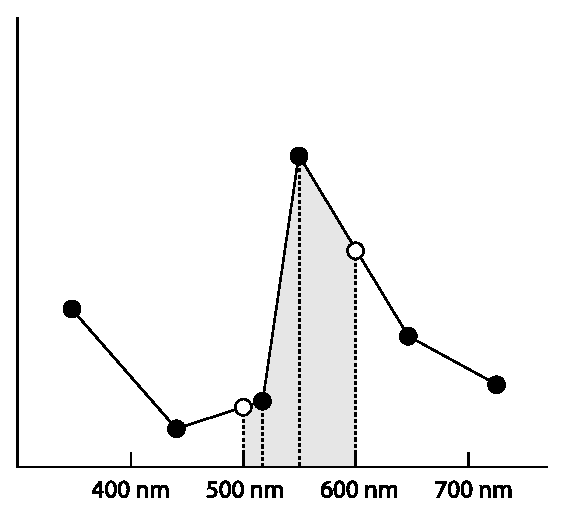
\includegraphics[width=0.4\linewidth]{chap05/IrregularSPDresample.eps}
    \caption{当重采样不规则定义的SPD时,我们需要计算由SPD样本定义的
        分段线性函数的均值。这里,我们想求从500nm到600nm的均值——图像下的阴影区。
        函数\refvar{AverageSpectrumSamples}{()}通过计算该图中虚线表示的每个区域的面积来完成。}
    \label{fig:5.2}
\end{figure}

\begin{lstlisting}
`\initcode{Spectrum Method Definitions}{=}\initnext{SpectrumMethodDefinitions}`
`\refvar{Float}{}` `\initvar{AverageSpectrumSamples}{}`(const `\refvar{Float}{}` *lambda, const `\refvar{Float}{}` *vals,
        int n, `\refvar{Float}{}` lambdaStart, `\refvar{Float}{}` lambdaEnd) {
    `\refcode{Handle cases with out-of-bounds range or single sample only}{}`
    `\refvar{Float}{}` sum = 0;
    `\refcode{Add contributions of constant segments before/after samples}{}`
    `\refcode{Advance to first relevant wavelength segment}{}`
    `\refcode{Loop over wavelength sample segments and add contributions}{}`
    return sum / (lambdaEnd - lambdaStart);
}
\end{lstlisting}

该函数从检查和处理极端情况开始,即求均值的波长范围
超出了提供的波长范围或只有单个样本进而均值计算是平凡的情况。
我们假设SPD在超出提供的采样范围外有常值(在两个端点的值);
如果这对于特定数据集不是一个合理的假设,则提供的数据应该在端点处有显式值(例如)0。
\begin{lstlisting}
`\initcode{Handle cases with out-of-bounds range or single sample only}{=}`
if (lambdaEnd   <= lambda[0])     return vals[0];
if (lambdaStart >= lambda[n - 1]) return vals[n - 1];
if (n == 1) return vals[0];
\end{lstlisting}

处理了这些情况后,下一步是检查看求均值的范围是否有部分超出第一个和/或最后一个样本值。
如果是,则我们累积常数段的贡献,用超出边界的波长范围缩放它。
\begin{lstlisting}
`\initcode{Add contributions of constant segments before/after samples}{=}`
if (lambdaStart < lambda[0])
    sum += vals[0] * (lambda[0] - lambdaStart);
if (lambdaEnd > lambda[n-1])
    sum += vals[n - 1] * (lambdaEnd - lambda[n - 1]);
\end{lstlisting}

现在我们推进到首个索引{\ttfamily i},
插值范围的起始波长重合于从$\lambda_i$到$\lambda_{i+1}$的一段。
这里更高效的实现是用二叉搜索而不是线性搜索
\footnote{甚至更高效的实现是利用一个事实即调用代码一般会需要
    在一段相邻波长范围上插值后的值,并可能在单次调用中接收了全部范围。
    然后可以为下一次插值从上一结尾处开始逐步寻找起始索引。}。
然而,该代码目前只在场景初始化时调用,所以目前不优化它不会影响渲染性能。
\begin{lstlisting}
`\initcode{Advance to first relevant wavelength segment}{=}`
int i = 0;
while (lambdaStart > lambda[i + 1]) ++i;
\end{lstlisting}

下面的循环在与求均值的范围重合的每个线性段上迭代。
对于每一段,它都通过求函数在这两点上取值的均值来
计算在波长范围{\ttfamily segLambdaStart}到{\ttfamily segLambdaEnd}上的均值。
该值依次用{\ttfamily interp()}计算,它是在给定波长的两个端点间线性插值的匿名函数。

下面的{\ttfamily std::min()}和{\ttfamily std::max()}调用计算波长范围以在该段内做平均;
注意它们自然地处理了{\ttfamily lambdaStart}、{\ttfamily lambdaEnd}或两者都在当前段内的情况。
\begin{lstlisting}
`\initcode{Loop over wavelength sample segments and add contributions}{=}`
auto interp = [lambda, vals](`\refvar{Float}{}` w, int i) {
    return `\refvar{Lerp}{}`((w - lambda[i]) / (lambda[i + 1] - lambda[i]),
                vals[i], vals[i + 1]);
};
for (; i+1 < n && lambdaEnd >= lambda[i]; ++i) {
    `\refvar{Float}{}` segLambdaStart = std::max(lambdaStart, lambda[i]);
    `\refvar{Float}{}` segLambdaEnd =   std::min(lambdaEnd,   lambda[i + 1]);
    sum += 0.5 * (interp(segLambdaStart, i) + interp(segLambdaEnd, i)) *
        (segLambdaEnd - segLambdaStart);
}
\end{lstlisting}

\subsection{XYZ颜色}\label{sub:XYZ颜色}
人类视觉系统的一个非凡性质是可只用三个浮点数为人类感知表示颜色。
颜色感知的\keyindex{三色刺激理论}{tristimulus theory}{}说
用三个值$x_{\lambda},y_{\lambda}$和$z_{\lambda}$就能为人类观察者准确表示所有可见SPD。
给定发射SPD即$S(\lambda)$,通过积分它们与\keyindex{光谱匹配曲线}{spectral matching curve}{}
$X(\lambda),Y(\lambda)$和$Z(\lambda)$的积可算得这些值:
\begin{align}\label{eq:5.1}
    x_{\lambda} & =\int\limits_{\lambda}{S(\lambda)X(\lambda)\mathrm{d}\lambda}\, ,\nonumber \\
    y_{\lambda} & =\int\limits_{\lambda}{S(\lambda)Y(\lambda)\mathrm{d}\lambda}\, ,          \\
    z_{\lambda} & =\int\limits_{\lambda}{S(\lambda)Z(\lambda)\mathrm{d}\lambda}\, .\nonumber
\end{align}

这些曲线是由国际照明委员会\sidenote{译者注:法文Commission Internationale de l'Éclairage,
    英文International Commission on Illumination,是有关光学、照明、颜色和色度空间科学领域的国际组织,成立于1913年。}(CIE)
规范化机构在一系列以人类为测试对象的实验后决定的并画于\reffig{5.3}中。
一般认为这些匹配曲线通常类似于人类视网膜中三种色敏视锥细胞\sidenote{译者注:原文 color-sensitive cone。}的响应。
惊人的是,有截然不同分布的SPD可能有非常接近的$x_{\lambda},y_{\lambda}$和$z_{\lambda}$值。
对于人类观察者,这样的SPD实际上有一样的视觉呈现。
这样的光谱对称为\keyindex{条件等色}{metamer}{}。
\begin{figure}[htbp]
    \centering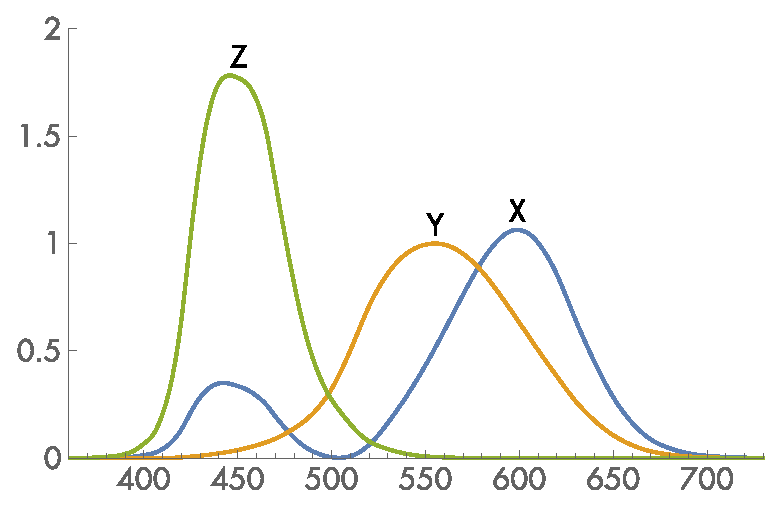
\includegraphics[width=0.5\linewidth]{chap05/matching-xyz.eps}
    \caption{对任意SPD计算XYZ值。用\refeq{5.1}让SPD与三个匹配曲线的每一个
    相乘并在其非零范围上积分以计算$x_{\lambda},y_{\lambda}$和$z_{\lambda}$值。}
    \label{fig:5.3}
\end{figure}

这给我们带来了关于光谱功率分布表示的一个微妙之处。
大部分颜色空间都希望模型颜色是对人类可见的,进而根据颜色感知的三色刺激理论只需用三个系数。
尽管XYZ能很好地表示要对人类观察者显示的给定SPD,
但它对于光谱计算而言{\itshape 不是}特别好的基函数集。
例如,尽管XYZ值能很好地分别描述柠檬皮或荧光灯的感知颜色(回想\reffig{5.1}),
但它们各自的XYZ值之积给出的XYZ颜色可能明显不同于用其SPD更精确的表示相乘再计算出的XYZ值。

pbrt提供了标准$X(\lambda),Y(\lambda)$和$Z(\lambda)$相应曲线从360nm到830nm间隔1nm采样的值。
下面的数组中第$i$个样本的波长由\refvar{CIE\_lambda}{}的第$i$个元素给定;
用这种方式显式表示样本波长能更容易将XYZ样本传入到像\refvar{AverageSpectrumSamples}{()}
那样接收波长数组作为参数的函数。
\begin{lstlisting}
`\initcode{Spectral Data Declarations}{=}\initnext{SpectralDataDeclarations}`
static const int `\initvar{nCIESamples}{}` = 471;
extern const `\refvar{Float}{}` `\initvar{CIE\_X}{}`[`\refvar{nCIESamples}{}`];
extern const `\refvar{Float}{}` `\initvar{CIE\_Y}{}`[`\refvar{nCIESamples}{}`];
extern const `\refvar{Float}{}` `\initvar{CIE\_Z}{}`[`\refvar{nCIESamples}{}`];
extern const `\refvar{Float}{}` `\initvar{CIE\_lambda}{}`[`\refvar{nCIESamples}{}`];
\end{lstlisting}

\refvar{SampledSpectrum}{}用这些样本计算其光谱表示里的XYZ匹配曲线(即它们自己是\refvar{SampledSpectrum}{})。
\begin{lstlisting}
`\initcode{SampledSpectrum Private Data}{=}\initnext{SampledSpectrumPrivateData}`
static `\refvar{SampledSpectrum}{}` `\initvar[SampledSpectrum::X]{X}{}`, `\initvar[SampledSpectrum::Y]{Y}{}`, `\initvar[SampledSpectrum::Z]{Z}{}`;
\end{lstlisting}

\refvar{SampledSpectrum}{}的XYZ曲线在方法\refvar{SampledSpectrum::Init}{()}中算得,
它在系统启动时被定义于\refsec{初始化和渲染选项}\sidenote{译者注:原文标错了章节,已修正。}
的函数\refvar{pbrtInit}{()}调用。
\begin{lstlisting}
`\refcode{SampledSpectrum Public Methods}{+=}\lastnext{SampledSpectrumPublicMethods}`
static void `\initvar[SampledSpectrum::Init]{Init}{}`() {
    `\refcode{Compute XYZ matching functions for SampledSpectrum}{}`
    `\refcode{Compute RGB to spectrum functions for SampledSpectrum}{}`
}
\end{lstlisting}
\begin{lstlisting}
`\initcode{General pbrt Initialization}{=}`
`\refvar{SampledSpectrum}{}`::`\refvar[SampledSpectrum::Init]{Init}{}`();
\end{lstlisting}

为\refvar{SampledSpectrum}{}给定波长范围和样本数量,
为每个样本计算匹配函数的值只需计算样本的波长范围并利用\refvar{AverageSpectrumSamples}{()}例程。
\begin{lstlisting}
`\initcode{Compute XYZ matching functions for SampledSpectrum}{=}`
for (int i = 0; i < `\refvar{nSpectralSamples}{}`; ++i) {
    `\refvar{Float}{}` wl0 = `\refvar{Lerp}{}`(`\refvar{Float}{}`(i) / `\refvar{Float}{}`(`\refvar{nSpectralSamples}{}`), 
                     `\refvar{sampledLambdaStart}{}`, `\refvar{nSpectralSamples}{}`);
    `\refvar{Float}{}` wl1 = `\refvar{Lerp}{}`(`\refvar{Float}{}`(i + 1) / `\refvar{Float}{}`(`\refvar{nSpectralSamples}{}`), 
                     `\refvar{sampledLambdaStart}{}`, `\refvar{sampledLambdaEnd}{}`);
    `\refvar[SampledSpectrum::X]{X}{}`.`\refvar[CoefficientSpectrum::c]{c}{}`[i] = `\refvar{AverageSpectrumSamples}{}`(`\refvar{CIE\_lambda}{}`, `\refvar{CIE\_X}{}`, `\refvar{nCIESamples}{}`,
                                    wl0, wl1);
    `\refvar[SampledSpectrum::Y]{Y}{}`.`\refvar[CoefficientSpectrum::c]{c}{}`[i] = `\refvar{AverageSpectrumSamples}{}`(`\refvar{CIE\_lambda}{}`, `\refvar{CIE\_Y}{}`, `\refvar{nCIESamples}{}`,
                                    wl0, wl1);
    `\refvar[SampledSpectrum::Z]{Z}{}`.`\refvar[CoefficientSpectrum::c]{c}{}`[i] = `\refvar{AverageSpectrumSamples}{}`(`\refvar{CIE\_lambda}{}`, `\refvar{CIE\_Z}{}`, `\refvar{nCIESamples}{}`,
                                    wl0, wl1);
}
\end{lstlisting}

pbrt中所有\refvar{Spectrum}{}实现都必须提供将其SPD转换为$(x_{\lambda},y_{\lambda},z_{\lambda})$系数的方法。
例如,在更新图像像素的过程中就会调用该方法。
当\refvar{Spectrum}{}表示的沿相机射出的光线上的光提供给\refvar{Film}{}时,
\refvar{Film}{}最终将它们转换为用于存储和/或显示的RGB值时处理的第一步就是将SPD转换为XYZ系数。

为了计算XYZ系数,\refvar{SampledSpectrum}{}用黎曼和计算\refeq{5.1}的积分:
\begin{align*}
    x_{\lambda}\approx\frac{\lambda_{\text{end}}-\lambda_{\text{start}}}{N}\sum\limits_{i=0}^{N-1}{X_ic_i}\, ,
\end{align*}
并以此类推。
\begin{lstlisting}
`\refcode{SampledSpectrum Public Methods}{+=}\lastnext{SampledSpectrumPublicMethods}`
void `\initvar{ToXYZ}{}`(`\refvar{Float}{}` xyz[3]) const {
    xyz[0] = xyz[1] = xyz[2] = 0.f;
    for (int i = 0; i < `\refvar{nSpectralSamples}{}`; ++i) {
        xyz[0] += `\refvar[SampledSpectrum::X]{X}{}`.`\refvar[CoefficientSpectrum::c]{c}{}`[i] * `\refvar[CoefficientSpectrum::c]{c}{}`[i];
        xyz[1] += `\refvar[SampledSpectrum::Y]{Y}{}`.`\refvar[CoefficientSpectrum::c]{c}{}`[i] * `\refvar[CoefficientSpectrum::c]{c}{}`[i];
        xyz[2] += `\refvar[SampledSpectrum::Z]{Z}{}`.`\refvar[CoefficientSpectrum::c]{c}{}`[i] * `\refvar[CoefficientSpectrum::c]{c}{}`[i];
    }
    `\refvar{Float}{}` scale = `\refvar{Float}{}`(`\refvar{sampledLambdaEnd}{}` - `\refvar{sampledLambdaStart}{}`) /
                  `\refvar{Float}{}`(CIE_Y_integral * `\refvar{nSpectralSamples}{}`);
    xyz[0] *= scale;
    xyz[1] *= scale;
    xyz[2] *= scale;
}
\end{lstlisting}

XYZ颜色的$y$系数与\keyindex{亮度}{luminance}{}密切相关,
它度量颜色的感知亮度\sidenote{译者注:原文brightness。}。
亮度将在\refsub{亮度和光度学}详细介绍。
我们提供了分开的方法单独计算$y$,因为经常只需要光谱的亮度
(例如第\refchap{光传输I:表面反射}、\refchap{光传输II:体积渲染}和\refchap{光传输III:双向方法}中的
一些光传输算法用亮度作为穿过场景的光路的相对重要性度量)。
\begin{lstlisting}
`\refcode{SampledSpectrum Public Methods}{+=}\lastnext{SampledSpectrumPublicMethods}`
`\refvar{Float}{}` `\initvar[SampledSpectrum::y]{y}{}`() const { 
    `\refvar{Float}{}` yy = 0.f;
    for (int i = 0; i < `\refvar{nSpectralSamples}{}`; ++i)
        yy += `\refvar[SampledSpectrum::Y]{Y}{}`.`\refvar[CoefficientSpectrum::c]{c}{}`[i] * `\refvar[CoefficientSpectrum::c]{c}{}`[i];
    return yy * `\refvar{Float}{}`(`\refvar{sampledLambdaEnd}{}` - `\refvar{sampledLambdaStart}{}`) /
        `\refvar{Float}{}`(`\refvar{nSpectralSamples}{}`);
}
\end{lstlisting}

\subsection{RGB颜色}\label{sub:RGB颜色}

\begin{lstlisting}
`\initcode{Compute RGB to spectrum functions for SampledSpectrum}{=}`
for (int i = 0; i < `\refvar{nSpectralSamples}{}`; ++i) {
    `\refvar{Float}{}` wl0 = `\refvar{Lerp}{}`(`\refvar{Float}{}`(i) / `\refvar{Float}{}`(`\refvar{nSpectralSamples}{}`), 
                     `\refvar{sampledLambdaStart}{}`, `\refvar{sampledLambdaEnd}{}`);
    `\refvar{Float}{}` wl1 = `\refvar{Lerp}{}`(`\refvar{Float}{}`(i+1) / `\refvar{Float}{}`(`\refvar{nSpectralSamples}{}`), 
                     `\refvar{sampledLambdaStart}{}`, `\refvar{sampledLambdaEnd}{}`);
    `\refvar{rgbRefl2SpectWhite}{}`.`\refvar[CoefficientSpectrum::c]{c}{}`[i] = `\refvar{AverageSpectrumSamples}{}`(`\refvar{RGB2SpectLambda}{}`, `\refvar{rgbRefl2SpectWhite}{}`, 
        `\refvar{nRGB2SpectSamples}{}`, wl0, wl1);
    `\refvar{rgbRefl2SpectCyan}{}`.`\refvar[CoefficientSpectrum::c]{c}{}`[i] = `\refvar{AverageSpectrumSamples}{}`(`\refvar{RGB2SpectLambda}{}`, `\refvar{rgbRefl2SpectCyan}{}`, 
        `\refvar{nRGB2SpectSamples}{}`, wl0, wl1);
    `\refvar{rgbRefl2SpectMagenta}{}`.`\refvar[CoefficientSpectrum::c]{c}{}`[i] = `\refvar{AverageSpectrumSamples}{}`(`\refvar{RGB2SpectLambda}{}`, `\refvar{rgbRefl2SpectMagenta}{}`, 
        `\refvar{nRGB2SpectSamples}{}`, wl0, wl1);
    `\refvar{rgbRefl2SpectYellow}{}`.`\refvar[CoefficientSpectrum::c]{c}{}`[i] = `\refvar{AverageSpectrumSamples}{}`(`\refvar{RGB2SpectLambda}{}`, `\refvar{rgbRefl2SpectYellow}{}`, 
        `\refvar{nRGB2SpectSamples}{}`, wl0, wl1);
    `\refvar{rgbRefl2SpectRed}{}`.`\refvar[CoefficientSpectrum::c]{c}{}`[i] = `\refvar{AverageSpectrumSamples}{}`(`\refvar{RGB2SpectLambda}{}`, `\refvar{rgbRefl2SpectRed}{}`, 
        `\refvar{nRGB2SpectSamples}{}`, wl0, wl1);
    `\refvar{rgbRefl2SpectGreen}{}`.`\refvar[CoefficientSpectrum::c]{c}{}`[i] = `\refvar{AverageSpectrumSamples}{}`(`\refvar{RGB2SpectLambda}{}`, `\refvar{rgbRefl2SpectGreen}{}`, 
        `\refvar{nRGB2SpectSamples}{}`, wl0, wl1);
    `\refvar{rgbRefl2SpectBlue}{}`.`\refvar[CoefficientSpectrum::c]{c}{}`[i] = `\refvar{AverageSpectrumSamples}{}`(`\refvar{RGB2SpectLambda}{}`, `\refvar{rgbRefl2SpectBlue}{}`, 
        `\refvar{nRGB2SpectSamples}{}`, wl0, wl1);

    `\refvar{rgbIllum2SpectWhite}{}`.`\refvar[CoefficientSpectrum::c]{c}{}`[i] = `\refvar{AverageSpectrumSamples}{}`(`\refvar{RGB2SpectLambda}{}`, `\refvar{rgbIllum2SpectWhite}{}`, 
        `\refvar{nRGB2SpectSamples}{}`, wl0, wl1);
    `\refvar{rgbIllum2SpectCyan}{}`.`\refvar[CoefficientSpectrum::c]{c}{}`[i] = `\refvar{AverageSpectrumSamples}{}`(`\refvar{RGB2SpectLambda}{}`, `\refvar{rgbIllum2SpectCyan}{}`, 
        `\refvar{nRGB2SpectSamples}{}`, wl0, wl1);
    `\refvar{rgbIllum2SpectMagenta}{}`.`\refvar[CoefficientSpectrum::c]{c}{}`[i] = `\refvar{AverageSpectrumSamples}{}`(`\refvar{RGB2SpectLambda}{}`, `\refvar{rgbIllum2SpectMagenta}{}`, 
        `\refvar{nRGB2SpectSamples}{}`, wl0, wl1);
    `\refvar{rgbIllum2SpectYellow}{}`.`\refvar[CoefficientSpectrum::c]{c}{}`[i] = `\refvar{AverageSpectrumSamples}{}`(`\refvar{RGB2SpectLambda}{}`, `\refvar{rgbIllum2SpectYellow}{}`, 
        `\refvar{nRGB2SpectSamples}{}`, wl0, wl1);
    `\refvar{rgbIllum2SpectRed}{}`.`\refvar[CoefficientSpectrum::c]{c}{}`[i] = `\refvar{AverageSpectrumSamples}{}`(`\refvar{RGB2SpectLambda}{}`, `\refvar{rgbIllum2SpectRed}{}`, 
        `\refvar{nRGB2SpectSamples}{}`, wl0, wl1);
    `\refvar{rgbIllum2SpectGreen}{}`.`\refvar[CoefficientSpectrum::c]{c}{}`[i] = `\refvar{AverageSpectrumSamples}{}`(`\refvar{RGB2SpectLambda}{}`, `\refvar{rgbIllum2SpectGreen}{}`, 
        `\refvar{nRGB2SpectSamples}{}`, wl0, wl1);
    `\refvar{rgbIllum2SpectBlue}{}`.`\refvar[CoefficientSpectrum::c]{c}{}`[i] = `\refvar{AverageSpectrumSamples}{}`(`\refvar{RGB2SpectLambda}{}`, `\refvar{rgbIllum2SpectBlue}{}`, 
        `\refvar{nRGB2SpectSamples}{}`, wl0, wl1);
}
\end{lstlisting}

\section{RGBSpectrum的实现}\label{sec:RGBSpectrum的实现}


{\noindent\hfil$=========$\hfil{\color{red}{施工分割线}}\hfil$=========$\
\section{辐射学}\label{sec:辐射学}

\section{表面反射}\label{sec:表面反射}

\subsection{BRDF}\label{sub:BRDF}

\subsection{BSSRDF}\label{sub:BSSRDF}

\chapter{相机模型}\label{chap:相机模型}

\section{逼真相机}\label{sec:逼真相机}
\begin{remark}
    本节含有高级内容,第一次阅读时可以跳过。
\end{remark}

薄透镜模型使得能渲染因景深而模糊的图像,
但它只是对多个\keyindex{透镜元件}{lens element}{}构成的
真实相机透镜系统非常粗糙的近似,而每个透镜元件都会改变穿过它的辐射分布
(\reffig{6.15}展示了具有8个元件的22mm焦距\keyindex{广角}{wide-angle}{}镜头横截面)。
即使基本的手机相机也趋于有五个左右独立的透镜元件,
而\keyindex{数码单镜头反光相机}{digital single-lens reflex camera}{camera相机}
(数码单反相机,DSLR)镜头可能有十个或更多。
通常,具备更大数量透镜元件的更复杂透镜系统能
比更简单的透镜系统创建更高质量的图像。
\begin{figure}[htbp]
    \centering%LaTeX with PSTricks extensions
%%Creator: Inkscape 1.1.1 (3bf5ae0d25, 2021-09-20)
%%Please note this file requires PSTricks extensions
\psset{xunit=.5pt,yunit=.5pt,runit=.5pt}
\begin{pspicture}(480,210.66666667)
{
\newrgbcolor{curcolor}{0 0 0}
\pscustom[linewidth=1.33333333,linecolor=curcolor]
{
\newpath
\moveto(102.07812533,200.869792)
\curveto(80.78645867,139.869792)(80.78645867,73.46354133)(102.07812533,12.46354133)
}
}
{
\newrgbcolor{curcolor}{0 0 0}
\pscustom[linewidth=1.33333333,linecolor=curcolor]
{
\newpath
\moveto(102.125,200.34895867)
\lineto(129.375,200.34895867)
}
}
{
\newrgbcolor{curcolor}{0 0 0}
\pscustom[linewidth=1.33333333,linecolor=curcolor]
{
\newpath
\moveto(102.125,11.942708)
\lineto(129.375,11.942708)
}
}
{
\newrgbcolor{curcolor}{0 0 0}
\pscustom[linewidth=1.33333333,linecolor=curcolor]
{
\newpath
\moveto(129.375,200.34895867)
\lineto(129.375,177.625)
}
}
{
\newrgbcolor{curcolor}{0 0 0}
\pscustom[linewidth=1.33333333,linecolor=curcolor]
{
\newpath
\moveto(129.375,11.942708)
\lineto(129.375,34.66145867)
}
}
{
\newrgbcolor{curcolor}{0 0 0}
\pscustom[linewidth=1.33333333,linecolor=curcolor]
{
\newpath
\moveto(129.95833333,178.14583333)
\curveto(108.70312533,160.494792)(96.41145867,134.29687467)(96.41145867,106.66666667)
\curveto(96.41145867,79.03645867)(108.70312533,52.83854133)(129.95833333,35.1875)
}
}
{
\newrgbcolor{curcolor}{0 0 0}
\pscustom[linewidth=1.33333333,linecolor=curcolor]
{
\newpath
\moveto(187.03125067,155.77604133)
\curveto(170.58854133,125.09895867)(170.58854133,88.23437467)(187.03125067,57.557292)
}
}
{
\newrgbcolor{curcolor}{0 0 0}
\pscustom[linewidth=1.33333333,linecolor=curcolor]
{
\newpath
\moveto(187.5625,155.255208)
\lineto(211.682292,155.255208)
}
}
{
\newrgbcolor{curcolor}{0 0 0}
\pscustom[linewidth=1.33333333,linecolor=curcolor]
{
\newpath
\moveto(187.5625,57.03125067)
\lineto(211.682292,57.03125067)
}
}
{
\newrgbcolor{curcolor}{0 0 0}
\pscustom[linewidth=1.33333333,linecolor=curcolor]
{
\newpath
\moveto(211.682292,155.255208)
\lineto(211.682292,145.119792)
}
}
{
\newrgbcolor{curcolor}{0 0 0}
\pscustom[linewidth=1.33333333,linecolor=curcolor]
{
\newpath
\moveto(211.682292,57.03125067)
\lineto(211.682292,67.17187467)
}
}
{
\newrgbcolor{curcolor}{0 0 0}
\pscustom[linewidth=1.33333333,linecolor=curcolor]
{
\newpath
\moveto(211.52604133,67.692708)
\curveto(217.22916667,93.364584)(217.22916667,119.96874933)(211.52604133,145.64062533)
}
}
{
\newrgbcolor{curcolor}{0 0 0}
\pscustom[linewidth=1.33333333,linecolor=curcolor]
{
\newpath
\moveto(211.682292,145.119792)
\lineto(231.1875,145.119792)
}
}
{
\newrgbcolor{curcolor}{0 0 0}
\pscustom[linewidth=1.33333333,linecolor=curcolor]
{
\newpath
\moveto(211.682292,67.17187467)
\lineto(231.1875,67.17187467)
}
}
{
\newrgbcolor{curcolor}{0 0 0}
\pscustom[linewidth=1.33333333,linecolor=curcolor]
{
\newpath
\moveto(231.1875,145.119792)
\lineto(231.1875,142.5)
}
}
{
\newrgbcolor{curcolor}{0 0 0}
\pscustom[linewidth=1.33333333,linecolor=curcolor]
{
\newpath
\moveto(231.1875,67.17187467)
\lineto(231.1875,69.79166667)
}
}
{
\newrgbcolor{curcolor}{0 0 0}
\pscustom[linewidth=1.33333333,linecolor=curcolor]
{
\newpath
\moveto(231.33333333,143.02083333)
\curveto(229.77083333,118.807292)(229.77083333,94.52604133)(231.33333333,70.3125)
}
}
{
\newrgbcolor{curcolor}{0 0 0}
\pscustom[linewidth=2.66666667,linecolor=curcolor]
{
\newpath
\moveto(236.510416,140.92708267)
\lineto(236.510416,175.70312533)
}
}
{
\newrgbcolor{curcolor}{0 0 0}
\pscustom[linewidth=2.66666667,linecolor=curcolor]
{
\newpath
\moveto(236.510416,71.364584)
\lineto(236.510416,36.58333333)
}
}
{
\newrgbcolor{curcolor}{0 0 0}
\pscustom[linewidth=1.33333333,linecolor=curcolor]
{
\newpath
\moveto(247.53125067,74.15625067)
\curveto(257.25,94.739584)(257.25,118.59374933)(247.53125067,139.17708267)
}
}
{
\newrgbcolor{curcolor}{0 0 0}
\pscustom[linewidth=1.33333333,linecolor=curcolor]
{
\newpath
\moveto(247.32291733,142.5)
\lineto(266.23437467,142.5)
}
}
{
\newrgbcolor{curcolor}{0 0 0}
\pscustom[linewidth=1.33333333,linecolor=curcolor]
{
\newpath
\moveto(247.32291733,69.79166667)
\lineto(266.23437467,69.79166667)
}
}
{
\newrgbcolor{curcolor}{0 0 0}
\pscustom[linewidth=1.33333333,linecolor=curcolor]
{
\newpath
\moveto(247.32291733,142.5)
\lineto(247.32291733,138.65104133)
}
}
{
\newrgbcolor{curcolor}{0 0 0}
\pscustom[linewidth=1.33333333,linecolor=curcolor]
{
\newpath
\moveto(247.32291733,69.79166667)
\lineto(247.32291733,73.635416)
}
}
{
\newrgbcolor{curcolor}{0 0 0}
\pscustom[linewidth=1.33333333,linecolor=curcolor]
{
\newpath
\moveto(265.98437467,70.3125)
\curveto(276.25,93.46354133)(276.25,119.869792)(265.98437467,143.02083333)
}
}
{
\newrgbcolor{curcolor}{0 0 0}
\pscustom[linewidth=1.33333333,linecolor=curcolor]
{
\newpath
\moveto(273.57812533,64.369792)
\curveto(274.47916667,92.5625)(274.47916667,120.77083333)(273.57812533,148.96354133)
}
}
{
\newrgbcolor{curcolor}{0 0 0}
\pscustom[linewidth=1.33333333,linecolor=curcolor]
{
\newpath
\moveto(274.17187467,151.58854133)
\lineto(278.78125067,151.58854133)
}
}
{
\newrgbcolor{curcolor}{0 0 0}
\pscustom[linewidth=1.33333333,linecolor=curcolor]
{
\newpath
\moveto(274.17187467,60.70312533)
\lineto(278.78125067,60.70312533)
}
}
{
\newrgbcolor{curcolor}{0 0 0}
\pscustom[linewidth=1.33333333,linecolor=curcolor]
{
\newpath
\moveto(274.17187467,151.58854133)
\lineto(274.17187467,148.442708)
}
}
{
\newrgbcolor{curcolor}{0 0 0}
\pscustom[linewidth=1.33333333,linecolor=curcolor]
{
\newpath
\moveto(274.17187467,60.70312533)
\lineto(274.17187467,63.84895867)
}
}
{
\newrgbcolor{curcolor}{0 0 0}
\pscustom[linewidth=1.33333333,linecolor=curcolor]
{
\newpath
\moveto(278.3125,61.22395867)
\curveto(291.4375,72.67708267)(298.97395867,89.244792)(298.97395867,106.66666667)
\curveto(298.97395867,124.08854133)(291.4375,140.65625067)(278.3125,152.10937467)
}
}
{
\newrgbcolor{curcolor}{0 0 0}
\pscustom[linewidth=1.33333333,linecolor=curcolor]
{
\newpath
\moveto(278.78125067,154.90625067)
\lineto(300.739584,154.90625067)
}
}
{
\newrgbcolor{curcolor}{0 0 0}
\pscustom[linewidth=1.33333333,linecolor=curcolor]
{
\newpath
\moveto(278.78125067,57.385416)
\lineto(300.739584,57.385416)
}
}
{
\newrgbcolor{curcolor}{0 0 0}
\pscustom[linewidth=1.33333333,linecolor=curcolor]
{
\newpath
\moveto(278.78125067,154.90625067)
\lineto(278.78125067,151.58854133)
}
}
{
\newrgbcolor{curcolor}{0 0 0}
\pscustom[linewidth=1.33333333,linecolor=curcolor]
{
\newpath
\moveto(278.78125067,57.385416)
\lineto(278.78125067,60.70312533)
}
}
{
\newrgbcolor{curcolor}{0 0 0}
\pscustom[linewidth=1.33333333,linecolor=curcolor]
{
\newpath
\moveto(301.28125067,57.90625067)
\curveto(313.60937467,89.244792)(313.60937467,124.08854133)(301.28125067,155.42708267)
}
}
{
\newrgbcolor{curcolor}{0 0 0}
\pscustom[linewidth=1.33333333,linecolor=curcolor]
{
\newpath
\moveto(310.05208267,53.35937467)
\curveto(329.29166667,64.20833333)(341.192708,84.57812533)(341.192708,106.66666667)
\curveto(341.192708,128.755208)(329.29166667,149.125)(310.05208267,159.97395867)
}
}
{
\newrgbcolor{curcolor}{0 0 0}
\pscustom[linewidth=1.33333333,linecolor=curcolor]
{
\newpath
\moveto(310.46354133,177.625)
\lineto(318.90104133,177.625)
}
}
{
\newrgbcolor{curcolor}{0 0 0}
\pscustom[linewidth=1.33333333,linecolor=curcolor]
{
\newpath
\moveto(310.46354133,34.66145867)
\lineto(318.90104133,34.66145867)
}
}
{
\newrgbcolor{curcolor}{0 0 0}
\pscustom[linewidth=1.33333333,linecolor=curcolor]
{
\newpath
\moveto(310.46354133,177.625)
\lineto(310.46354133,159.45312533)
}
}
{
\newrgbcolor{curcolor}{0 0 0}
\pscustom[linewidth=1.33333333,linecolor=curcolor]
{
\newpath
\moveto(310.46354133,34.66145867)
\lineto(310.46354133,52.83854133)
}
}
{
\newrgbcolor{curcolor}{0 0 0}
\pscustom[linewidth=1.33333333,linecolor=curcolor]
{
\newpath
\moveto(318.75,35.1875)
\curveto(339.32291733,53.244792)(351.114584,79.29166667)(351.114584,106.66666667)
\curveto(351.114584,134.04166667)(339.32291733,160.08854133)(318.75,178.14583333)
}
}
{
\newrgbcolor{curcolor}{0 0 0}
\pscustom[linewidth=1.33333333,linecolor=curcolor]
{
\newpath
\moveto(469.09374933,10.8125)
\lineto(469.09374933,201.47395867)
}
}
{
\newrgbcolor{curcolor}{0 0 0}
\pscustom[linewidth=1.33333333,linecolor=curcolor]
{
\newpath
\moveto(469.09374933,106.14583333)
\lineto(9.57291733,106.14583333)
}
}
\end{pspicture}

    \caption{广角透镜系统的横截面(在pbrt发行版的{\ttfamily scenes/lenses/wide.22mm.dat}
    中)。透镜坐标系统让胶片平面垂直于$z$轴且位于$z=0$处。
    透镜在左边负z轴上,然后场景在透镜左侧。透镜系统中部表示为粗黑线的光圈阻挡命中它的光线。
    在许多透镜系统中,可以调整光圈大小以在更短曝光时间(大光圈)和更大景深(小光圈)间权衡。}
    \label{fig:6.15}
\end{figure}

本节讨论\refvar{RealisticCamera}{}的实现,
它模拟光穿过像\reffig{6.15}那样的透镜系统后聚焦并渲染像\reffig{6.16}那样的图像。
其实现基于光线追踪,即相机追随光路穿过透镜元件,
并考虑具有不同折射率的介质(空气,各类玻璃)间界面的折射,
直到光路要么退出光学系统要么被光圈或镜头罩吸收。
离开前端镜头元件的光线代表相机响应曲线,可用于估计
沿任意光线入射辐亮度的积分器,例如\refvar{SamplerIntegrator}{}。
\refvar{RealisticCamera}{}的实现在文件\href{https://github.com/mmp/pbrt-v3/tree/master/src/cameras/realistic.h}{\ttfamily cameras/realistic.h}
和\href{https://github.com/mmp/pbrt-v3/tree/master/src/cameras/realistic.cpp}{\ttfamily cameras/realistic.cpp}中。
\begin{figure}[htbp]
    \centering\includegraphics[width=0.6\linewidth]{chap06/sanmiguel-fisheye.png}
    \caption{用鱼眼透镜和很宽视场渲染的图像。注意边缘暗处是
        准确模拟成像辐射度量(\refsub{相机测量方程})所致,
        而直线扭曲为曲线则是许多广角镜头的特点,但在用投影矩阵表示透镜投影模型时没有考虑。}
    \label{fig:6.16}
\end{figure}
\begin{lstlisting}
`\initcode{RealisticCamera Declarations}{=}`
class `\initvar{RealisticCamera}{}` : public `\refvar{Camera}{}` {
public:
    `\refcode{RealisticCamera Public Methods}{}`
private:
    `\refcode{RealisticCamera Private Declarations}{}`
    `\refcode{RealisticCamera Private Data}{}`
    `\refcode{RealisticCamera Private Methods}{}`
};
\end{lstlisting}

除了把相机放置于场景中的常见变换、\refvar{Film}{}以及快门打开和关闭的时间外,
\refvar{RealisticCamera}{}构造函数还接收透镜系统描述文件的文件名、
到期望的焦平面的距离以及光圈直径。之后有了第\refchap{蒙特卡洛积分}蒙特卡洛积分与
\refsub{相机测量方程}成像辐射度量的预备知识后,
将在\refsub{采样相机1}介绍参数{\ttfamily simpleWeighting}的作用。
\begin{lstlisting}
`\initcode{RealisticCamera Method Definitions}{=}\initnext{RealisticCameraMethodDefinitions}`
`\refvar{RealisticCamera}{}`::`\refvar{RealisticCamera}{}`(const `\refvar{AnimatedTransform}{}` &CameraToWorld,
        `\refvar{Float}{}` shutterOpen, `\refvar{Float}{}` shutterClose, `\refvar{Float}{}` apertureDiameter,
        `\refvar{Float}{}` focusDistance, bool simpleWeighting, const char *lensFile,
        `\refvar{Film}{}` *film, const `\refvar{Medium}{}` *medium)
    : `\refvar{Camera}{}`(CameraToWorld, shutterOpen, shutterClose, film, medium),
      simpleWeighting(simpleWeighting) {
    `\refcode{Load element data from lens description file}{}`
    `\refcode{Compute lens–film distance for given focus distance}{}`
    `\refcode{Compute exit pupil bounds at sampled points on the film}{}`
}
\end{lstlisting}
\begin{lstlisting}
`\initcode{Load element data from lens description file}{=}`
std::vector<`\refvar{Float}{}`> lensData;
if (ReadFloatFile(lensFile, &lensData) == false) {
    `\refvar{Error}{}`("Error reading lens specification file \"%s\".", lensFile);
    return;
}
if ((lensData.size() % 4) != 0) {
    `\refvar{Error}{}`("Excess values in lens specification file \"%s\"; "
          "must be multiple-of-four values, read %d.",
          lensFile, (int)lensData.size());
    return;
}
for (int i = 0; i < (int)lensData.size(); i += 4) {
    if (lensData[i] == 0) {
        if (apertureDiameter > lensData[i+3]) {
            `\refvar{Warning}{}`("Specified aperture diameter %f is greater than maximum "
                    "possible %f.  Clamping it.", apertureDiameter, lensData[i+3]);
        } else {
            lensData[i+3] = apertureDiameter;
        }
    }
    `\refvar{elementInterfaces}{}`.push_back((`\refvar{LensElementInterface}{}`)
        {lensData[i] * (`\refvar{Float}{}`).001, lensData[i+1] * (`\refvar{Float}{}`).001, lensData[i+2],
         lensData[i+3] * `\refvar{Float}{}`(.001) / `\refvar{Float}{}`(2.)});
}
\end{lstlisting}
\begin{lstlisting}
`\initcode{RealisticCamera Private Data}{=}\initnext{RealisticCameraPrivateData}`
const bool `\initvar{simpleWeighting}{}`;
\end{lstlisting}

在从磁盘加载透镜描述文件之后,构造函数调整透镜与
胶片间的距离使得焦平面位于期望的深度即{\ttfamily focusDistance},
然后预先计算一些关于离胶片最近透镜元件的哪部分面积让光从场景射到胶片的信息,
就像在胶片平面上各点看到的那样。在介绍完背景材料之后,
\refsub{对焦}和\refsub{出射瞳}将分别定义代码片
\refcode{Compute lens-film distance for given focus distance}{}
和\refcode{Compute exit pupil bounds at sampled points on the film}{}。

\subsection{透镜系统表示}\label{sub:透镜系统表示}
透镜系统由一系列透镜元件组成,每个元件通常是某种形制的玻璃。
透镜系统设计者的挑战是在有限空间、成本和生产难度下
设计一组能在胶片或传感器上高质量成像的元件
(例如为了让保持手机变薄,其相机厚度非常有限)。

最容易生产的是横截面为球形的透镜,
透镜系统通常是绕\keyindex{光轴}{optical axis}{}对称的,习惯记为$z$。
我们将假设这两个性质在本节下文中成立。
用胶片对齐到平面$z=0$且透镜在胶片左侧沿$-z$轴放置的坐标系统定义透镜系统。

透镜系统常表示为独立透镜元件(或空气)间的一系列界面,
而不是每个元件的显式表示。\reftab{6.1}展示了定义每个界面的量。
表中最后一项定义了最右边的界面,如\reffig{6.17}所示:
它是个半径等于曲率半径的球体块。元件的厚度是沿$z$到右边下一个
元件(或胶片平面)的距离,\keyindex{折射率}{index of refraction}{}是
对界面右边的介质而言的。元件在$z$轴上下的范围由光圈直径设置。
\begin{table}[htbp]
    \centering
    \begin{tabular}{SSSS}
        \toprule
        \ \ \ \textbf{曲率半径} & \ \ \ \ \textbf{厚度} & \ \textbf{折射率} & \textbf{光圈直径} \\
        \midrule
        35.98738                & 1.21638               & 1.54              & 23.716            \\
        11.69718                & 9.9957                & 1                 & 17.996            \\
        13.08714                & 5.12622               & 1.772             & 12.364            \\
        -22.63294               & 1.76924               & 1.617             & 9.812             \\
        71.05802                & 0.8184                & 1                 & 9.152             \\
        0                       & 2.27766               & 0                 & 8.756             \\
        -9.58584                & 2.43254               & 1.617             & 8.184             \\
        -11.28864               & 0.11506               & 1                 & 9.152             \\
        -166.7765               & 3.09606               & 1.713             & 10.648            \\
        -7.5911                 & 1.32682               & 1.805             & 11.44             \\
        -16.7662                & 3.98068               & 1                 & 12.276            \\
        -7.70286                & 1.21638               & 1.617             & 13.42             \\
        -11.97328               & (取决于焦点)        & 1                 & 17.996            \\
        \bottomrule
    \end{tabular}
    \caption{\reffig{6.15}中透镜系统的表格化描述。每行描述了两个透镜元件间的界面、
        元件与空气间的界面或者光圈。第一行描述了最左边的界面。半径为0的元件对应光圈。
        距离单位为mm。}
    \label{tab:6.1}
\end{table}
\begin{figure}[htbp]
    \centering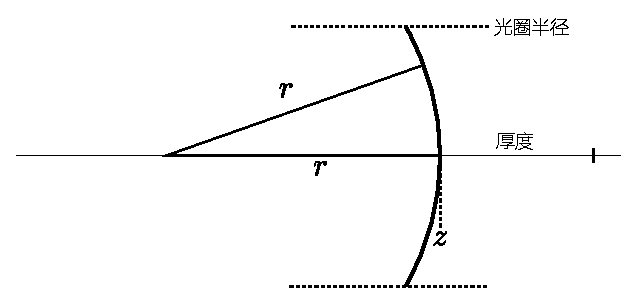
\includegraphics[width=0.6\linewidth]{chap06/Lenselement.eps}
    \caption{透镜界面(实曲线)与光轴相交于位置$z$。界面几何形状由
        表示其在光轴上下方范围的光圈半径以及元件的曲率半径$r$描述。
        如果元件有球形横截面,则它的轮廓由球心在光轴上距离$r$的球体给定,
        该球体也穿过$z$。如果$r$是负的,则元件界面就如从场景中看到那样是凹的
        (如图所示);否则就是\protect\keyindex{凸}{convex}{}的。透镜厚度给出了到
        右边下一个界面的距离,或者对于最右边的界面是到胶片平面的距离。}
    \label{fig:6.17}
\end{figure}

结构体\refvar{LensElementInterface}{}表示单个透镜元件界面。
\begin{lstlisting}
`\initcode{RealisticCamera Private Declarations}{=}`
struct `\initvar{LensElementInterface}{}` {
    `\refvar{Float}{}` `\initvar{curvatureRadius}{}`;
    `\refvar{Float}{}` `\initvar{thickness}{}`;
    `\refvar{Float}{}` `\initvar[LensElementInterface::eta]{eta}{}`;
    `\refvar{Float}{}` `\initvar{apertureRadius}{}`;
};
\end{lstlisting}

这里没有介绍的代码片\refcode{Load element data from lens description file}{}
\sidenote{译者注:我补充回来了。}读取透镜元件
并初始化数组\refvar[elementInterfaces]{RealisticCamera::elementInterfaces}{}。
见源代码中的注释了解该文件格式的细节,它并行化\reftab{6.1}中的结构,
并见pbrt发行版中的目录{\ttfamily scenes/lenses}了解大量透镜描述示例。

对从文件读取的值做了两个调整:第一,透镜系统传统上用毫米单位描述,
但pbrt假设场景单位用米。因此,除了折射率外的域都按1/1000缩小。
第二,元件直径被除以二;在下面的代码中半径是用起来更方便的量。
\begin{lstlisting}
`\refcode{RealisticCamera Private Data}{+=}\lastnext{RealisticCameraPrivateData}`
std::vector<`\refvar{LensElementInterface}{}`> `\initvar{elementInterfaces}{}`;
\end{lstlisting}

一旦加载完透镜界面描述,让一些关于透镜系统的值随时可得是很有用的。
\refvar{LensRearZ}{()}和\refvar{LensFrontZ}{()}分别返回
透镜系统尾部和头部元件的$z$深度。注意返回的$z$深度在相机空间中,
而不是透镜空间中,所以为正值。
\begin{lstlisting}
`\initcode{RealisticCamera Private Methods}{=}\initnext{RealisticCameraPrivateMethods}`
`\refvar{Float}{}` `\initvar{LensRearZ}{}`() const {
    return `\refvar{elementInterfaces}{}`.back().`\refvar{thickness}{}`;
}
\end{lstlisting}

求头部元件$z$位置需要求所有元件厚度之和(见\reffig{6.18})。
任何位于系统性能敏感部分的代码都不需要该值,
所以在需要时重算它就行。如果该方法对性能有影响,
最好还是在\refvar{RealisticCamera}{}中缓存该值。
\begin{figure}[htbp]
    \centering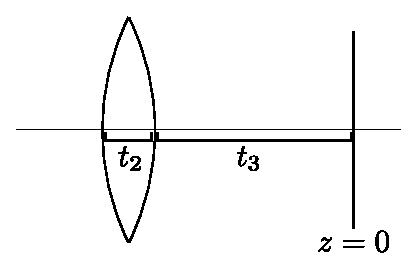
\includegraphics[width=0.4\linewidth]{chap06/Elementthicknessandposition.eps}
    \caption{元件厚度与光轴上位置的关系。胶片平面位于$z=0$,尾部元件的厚度$t_3$给出
        了从胶片到其界面的距离;这里尾部界面与轴交于$z=-t_3$。下一个元件厚度为$t_2$且
        位于$z=-t_3-t_2$,以此类推。头部元件交$z$轴于$\sum_i-t_i$。}
    \label{fig:6.18}
\end{figure}
\begin{lstlisting}
`\refcode{RealisticCamera Private Methods}{+=}\lastnext{RealisticCameraPrivateMethods}`
`\refvar{Float}{}` `\initvar{LensFrontZ}{}`() const {
    `\refvar{Float}{}` zSum = 0;
    for (const `\refvar{LensElementInterface}{}` &element : `\refvar{elementInterfaces}{}`)
        zSum += element.`\refvar{thickness}{}`;
    return zSum;
}
\end{lstlisting}

\refvar{RearElementRadius}{()}按单位米返回尾部元件光圈半径。
\begin{lstlisting}
`\refcode{RealisticCamera Private Methods}{+=}\lastnext{RealisticCameraPrivateMethods}`
`\refvar{Float}{}` `\initvar{RearElementRadius}{}`() const {
    return `\refvar{elementInterfaces}{}`.back().`\refvar{apertureRadius}{}`;
}
\end{lstlisting}
\subsection{追踪穿过透镜的光线}\label{sub:追踪穿过透镜的光线}

\subsection{厚透镜近似}\label{sub:厚透镜近似}
\subsection{对焦}\label{sub:对焦}
\subsection{出射瞳}\label{sub:出射瞳}
\subsection{相机测量方程}\label{sub:相机测量方程}

\chapterimage{Pictures/chap07/checkerboard-ref-465x930.png}
\chapter{采样与重构}\label{chap:采样与重构}
\setcounter{sidenote}{1}
尽管像pbrt那样的渲染器最终输出的是彩色像素的2D网格,
但实际上入射辐射是定义在胶片平面上的连续函数。
从该连续函数计算出离散像素值的方法会显著影响渲染器生成的最终图像的质量;
如果没有仔细执行该过程,则会出现伪影\sidenote{译者注:原文artifact。}。
反之,如果执行得很好,则为此进行相对少量的额外计算就能极大提升渲染图像的质量。

本章从介绍\emph{采样理论}开始——即从定义在连续域上的函数
取出离散样本值并用它们重建与原本类似的新函数的理论。
在采样理论和低偏差点集(一种均匀分布的样本点类型)思想的基础上,
本章定义的\refvar{Sampler}{}以不同方式生成$n$维样本向量
\footnote{回想上一章中\refvar{Camera}{}用\refvar{CameraSample}{}
在胶片平面、透镜上以及时间域中取点——通过取用这些样本向量前几维来设定\refvar{CameraSample}{}值。}。
本章将介绍五种\refvar{Sampler}{}实现,涵盖了采样问题的各种方法。

本章以类\refvar{Filter}{}和\refvar{Film}{}作结。
\refvar{Filter}{}用于确定每个像素周围要融合多少倍样本量来计算最终像素值,
类\refvar{Film}{}则积累图像样本对图中像素的贡献量。

\section{采样理论}\label{sec:采样理论}
数字图像表示为一组像素值,通常对齐到矩形网格。
当在物理设备上展示数字图像时,这些值用于确定显示器上像素发射的光谱功率。
当考虑数字图像时,区分图像像素与显示器像素很重要,
前者表示一个函数在特定样本位置的值,后者是具有某个发光分布的物理对象
(例如对于LCD显示器,当以倾斜角度观察它时,颜色和亮度可能会极大变化)。
显示器用图像像素值在显示器表面构造新的图像函数。
该函数定义在显示器所有点位上,而不只是数字图像像素的无穷小点上。
这样取一组样本值并将其转换回连续函数的过程称为\keyindex{重建}{reconstruction}{}。

为了计算数字图像中的离散像素值,必须采样原始连续定义的图像函数。
在pbrt中,像大多数其他光线追踪渲染器那样,
获取图像函数有关信息的唯一方法就是通过追踪光线来对其采样。
例如,能计算胶片平面上两点间的图像函数变化边界的通用方法是不存在的。
尽管可以通过在像素位置上精确采样该函数来生成图像,
但通过在不同位置上取用更多样本并将这些关于图像函数的
额外信息融合到最终的像素值中能得到更好的结果。
实际上,为了有最佳质量的结果,计算像素值时应使得
在显示设备上重建的图像尽可能与虚拟相机胶片平面上的场景原始图像逼近。
注意这和希望显示器像素在其位置上取用图像函数实际值的目标有些微妙区别。
处理这一区别是本章实现的算法的主要目标
\footnote{本书中我们将忽略物理显示器像素特性相关问题并
    在显示器执行本节后面所述理想重建过程的假设下处理。
    该假设显然与真实显示器的工作方式不符,但这里它避免了不必要的复杂分析。
    \citet{GLASSNER1995}的第3章很好地处理了非理想显示设备
    及其对图像采样和重建过程的影响。}。

因为采样和重建过程涉及估值,所以它引入了称作\keyindex{混叠}{aliasing}{}的误差,
并会以许多方式表现出来,包括锯齿状边缘或动画中的闪烁。
产生这些误差的原因是采样过程不能捕获来自连续定义的图像函数的全部信息。

作为这些思想的一个例子,考虑一个1D函数(我们也会称之为信号)即$f(x)$,
我们可以求函数定义域中任意期望位置$x'$处的值$f(x')$。
每个这样的$x'$称为\keyindex{样本位置}{sample position}{},
$f(x')$的值称为\keyindex{样本值}{sample value}{}。
\reffig{7.1}展示了光滑1D函数的样本集,以及逼近原始函数$f$的重建信号$\tilde{f}$。
本例中,$\tilde{f}$是分段线性函数,通过线性插值相邻样本值来逼近$f$
(已经熟悉采样理论的读者会认出这是用帽函数\sidenote{译者注:原文hat function。}重建的)。
因为关于$f$唯一可用的信息是来自在位置$x'$处的采样值,
且没有关于$f$在样本间特性的信息,所以$\tilde{f}$不能完全匹配$f$。
\begin{figure}[htbp]
    \centering
    \subfloat[]{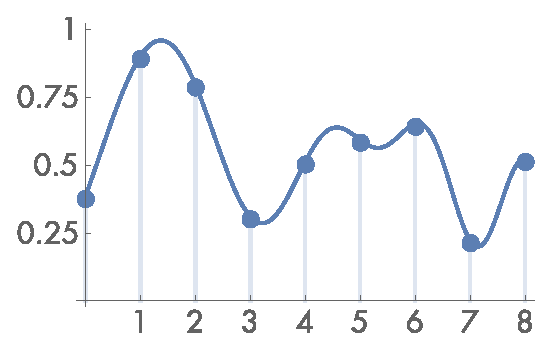
\includegraphics[width=0.4\linewidth]{chap07/point-sampling.eps}}\,\,
    \subfloat[]{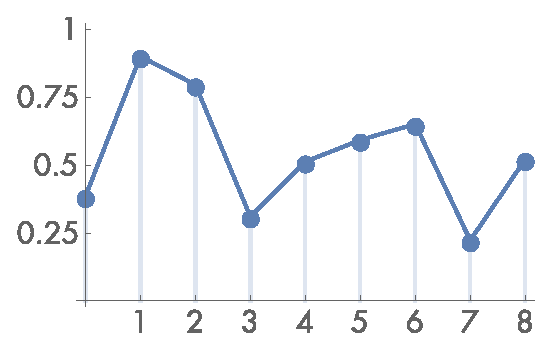
\includegraphics[width=0.4\linewidth]{chap07/linear-reconstruction.eps}}
    \caption{(a)通过取$f(x)$的\emph{样本点}集(标实心记),我们确定了函数在这些位置处的值。
        (b)样本值可用于\emph{重建}逼近$f(x)$的函数$\tilde{f}(x)$。
        \refsub{混叠}介绍的采样原理准确描述了关于$f(x)$的条件、
        所需样本的数目,以及使得$\tilde{f}(x)$和$f(x)$一模一样的重建技术。
        原始函数有时能只从样本点中完全重建的事实令人瞩目。}
    \label{fig:7.1}
\end{figure}

\keyindex{傅里叶分析}{Fourier analysis}{}可用于评估重建函数与原始函数间的匹配质量。
本节将用丰富细节来介绍一部分采样和重建过程中涉及的傅里叶分析主要思想,
但略去了许多性质的证明并跳过了与pbrt所用的采样算法没有直接关系的细节。
本章“扩展阅读”一节有关于这些话题详细信息的指引。

\subsection{频域与傅里叶变换}\label{sub:频域与傅里叶变换}
傅里叶分析的基础之一是\keyindex{傅里叶变换}{Fourier transform}{transform变换},
它在\keyindex{频域}{frequency domain}{}中来表示函数(我们称
通常的函数是在\keyindex{空域}{spatial domain}{}中表示的)。
考虑\reffig{7.2}中的两个函数。\reffig{7.2.1}中$x$的函数变化得相对较慢,
而\reffig{7.2.2}中的函数变化得迅速得多。称变化越慢的函数有越低频的分量。
\begin{figure}[htbp]
    \centering
    \subfloat[]{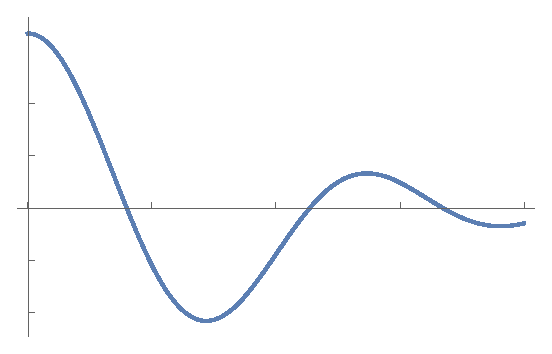
\includegraphics[width=0.32\linewidth]{chap07/func-lowfreq.eps}\label{fig:7.2.1}}\,\,\,\,
    \subfloat[]{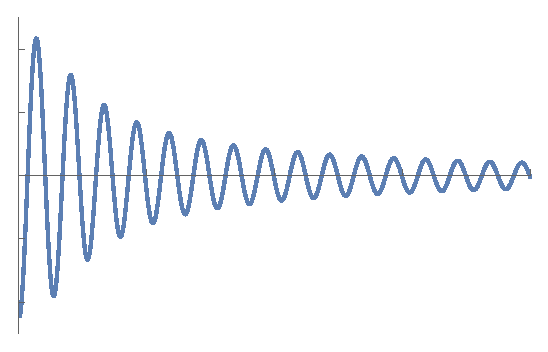
\includegraphics[width=0.32\linewidth]{chap07/func-highfreq.eps}\label{fig:7.2.2}}
    \caption{(a)低频函数和(b)高频函数。粗略地说,函数频率越高,在给定区域内变化得越快。}
    \label{fig:7.2}
\end{figure}

\reffig{7.3}展示了这两个函数在频率空间的表示;低频函数的表示比高频函数更快变为0。
\begin{figure}[htbp]
    \centering
    \subfloat[]{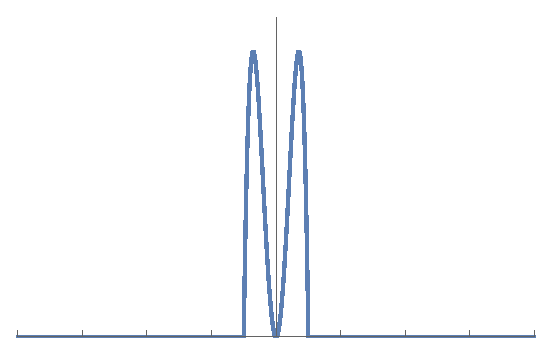
\includegraphics[width=0.32\linewidth]{chap07/fourier-lowfreq.eps}}\,\,\,\,
    \subfloat[]{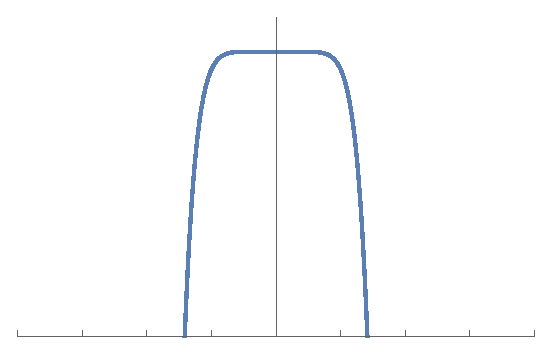
\includegraphics[width=0.32\linewidth]{chap07/fourier-highfreq.eps}}
    \caption{\reffig{7.2}中的函数的频率空间表示。本图展示了每个频率$\omega$对空域中每个函数的贡献。}
    \label{fig:7.3}
\end{figure}

许多函数可以分解为平移过的正弦曲线的加权和。
约瑟夫·傅里叶\sidenote{译者注:Jean-Baptiste Joseph Fourier,18至19世纪法国著名数学家和物理学家。}
首先描述了这一奇特事实,傅里叶变换即将函数转换为该表示。
函数的频率空间表示便于深入了解其一些特点——正弦函数的频率分布对应于原函数的频率分布。
使用该形式后,就能用傅里叶分析深入了解采样和重建过程引入的误差以及如何降低该误差带来的感知影响。

1D函数$f(x)$的傅里叶变换为\footnote{要告知读者的是,
    在不同领域中该积分前的常数并不总是一样的。例如一些作者(包括许多物理界的)
    更喜欢在两个积分前乘上$\frac{1}{\sqrt{2\pi}}$。}
\begin{align}\label{eq:7.1}
    F(\omega)=\int_{-\infty}^{\infty}f(x)\mathrm{e}^{-\mathrm{i}2\pi\omega x}\mathrm{d}x\, .
\end{align}
(回想$\mathrm{e}^{-\mathrm{i}x}=\cos x+\mathrm{i}\sin x$,其中$\mathrm{i}=\sqrt{-1}$。)
为了简便,这里我们将只考虑\keyindex{偶函数}{even function}{},
即$f(-x)=f(x)$,这种情况下$f$的傅里叶变换没有虚数项。
新函数$F$是\keyindex{频率}{frequency}{}$\omega$的函数
\footnote{本章中,我们将用符号$\omega$表示频率。在本书剩下部分中,$\omega$表示规范化的方向向量。
    这种记号的重复在使用它们的给定上下文中不应混淆。简单来说,当我们说函数的“频谱”(spectrum)时,
    我们是在说它在其频率空间表示中的频率分布,而不是和颜色相关的东西。}。
我们将用$\mathcal{F}$表示傅里叶变换运算
\sidenote{译者注:原文使用的符号是$\mathrm{F}$,这里译者换用更常用的花体$\mathcal{F}$,
    也更利于阅读时与其他符号区分。},即$\mathcal{F}\{f(x)\}=F(\omega)$。
$\mathcal{F}$显然是线性运算——即对任意标量$a$都有$\mathcal{F}\{af(x)\}=a\mathcal{F}\{f(x)\}$,
且$\mathcal{F}\{f(x)+g(x)\}=\mathcal{F}\{f(x)\}+\mathcal{F}\{g(x)\}$。

\refeq{7.1}称为\keyindex{傅里叶分析}{Fourier analysis}{}方程,有时简称\keyindex{傅里叶变换}{Fourier transform}{transform变换}。
我们也可用\keyindex{傅里叶合成}{Fourier synthesis}{}方程从频域变换回空域,
也称作\keyindex{傅里叶逆变换}{inverse Fourier transform}{transform变换}
\sidenote{译者注:大多数文献采用的傅里叶变换或逆变换定义中$\omega$是角频率,但本书的定义中$\omega$是频率。}:
\begin{align}\label{eq:7.2}
    f(x)=\int_{-\infty}^{\infty}F(\omega)\mathrm{e}^{\mathrm{i}2\pi\omega x}\mathrm{d}\omega\, .
\end{align}

\reftab{7.1}展示了许多重要函数及其频率空间表示
\sidenote{译者注:表中原文将频域函数写作$f(\omega)$,译者改为了$F(\omega)$。
    此外,表中原文对余弦函数和Shah函数的频域表示混用了系数不同的傅里叶变换定义,
    导致与本书所采用的定义不符,译者已根据本书定义对其作了修正。
    具体推导过程可参考译者补充的\refsec{译者补充:信号处理}。}。
这些函数中许多都基于狄拉克$\delta$分布
\sidenote{译者注:也称作单位\keyindex{冲激函数}{impulse function}{}、脉冲函数。},
该空间函数的定义使得$\displaystyle\int\delta(x)\mathrm{d}x=1$,且对任意$x\neq0$,都有$\delta(x)=0$。
这些性质的一个重要结论是
\begin{align*}
    \int f(x)\delta(x)\mathrm{d}x=f(0)\, .
\end{align*}

$\delta$分布不能表示为标准数学函数\sidenote{译者注:也就是说冲激函数是一种奇异函数。},
但通常可以视作以原点为中心且宽度逼近0的单位面积矩形函数\sidenote{译者注:原文box function。}的极限。
\begin{table}[htbp]
    \centering\begin{tabular}{l p{170pt}}
        \toprule
        {\bfseries 空域}                                                   & {\bfseries 频率空间表示}                                                                     \\
        \midrule
        矩形函数:$f(x)=\left\{\begin{array}{ll}
                1, & \text{若}|x|<\frac{1}{2}, \\
                0, & \text{其他}.
            \end{array}\right.$           & Sinc函数:$\displaystyle F(\omega)=\mathrm{sinc}(\omega)=\frac{\sin(\pi\omega)}{\pi\omega}$  \\
        \hline
        高斯函数:$f(x)=\mathrm{e}^{-\pi x^2}$                             & 高斯函数:$F(\omega)=\mathrm{e}^{-\pi \omega^2}$                                             \\
        \hline
        常函数:$f(x)=1$                                                   & $\delta$函数:$F(\omega)=\delta(\omega)$                                                     \\
        \hline
        余弦函数:$f(x)=\cos x$                                            & 平移的$\delta$函数:
        $F(\omega)=\frac{1}{2}(\delta(1-2\pi\omega)+\delta(1+2\pi\omega))$                                                                                                \\
        \hline
        Shah函数:$\displaystyle f(x)=III_T(x)=T\sum\limits_k\delta(x-kT)$ & $\displaystyle F(\omega)=TIII_{\frac{1}{T}}(\omega)=\sum\limits_k\delta(\omega-\frac{k}{T})$ \\
        \bottomrule
    \end{tabular}
    \caption{傅里叶变换对。空域中的函数及其频率空间表示。
        因为傅里叶变换的对称性,如果左边一列被当作频率空间,
        则右边一列是这些函数的空间等价。}
    \label{tab:7.1}
\end{table}

\subsection{理想采样与重建}\label{sub:理想采样与重建}

\subsection{混叠}\label{sub:混叠}

\section{采样接口}\label{sec:采样接口}

\subsection{基本采样器接口}\label{sub:基本采样器接口}

\begin{lstlisting}
`\initcode{Sampler Declarations}{=}\initnext{SamplerDeclarations}`
class `\initvar{Sampler}{}` {
public:
    `\refcode{Sampler Interface}{}`
    `\refcode{Sampler Public Data}{}`
protected:
    `\refcode{Sampler Protected Data}{}`
private:
    `\refcode{Sampler Private Data}{}`
};
\end{lstlisting}

\section{分层采样}\label{sec:分层采样}
我们将要介绍的首个\refvar{Sampler}{}实现会把
像素区域细分为矩形区域并在每个区域内生成单个样本。
这些区域常称为\keyindex{层}{strata}{},
而该采样器称为\refvar{StratifiedSampler}{}。
分层背后的关键思想是通过把采样域细分为不重叠区域
并从每个中取单个样本,我们更不可能错失整个图像的重要特征,
因为保证了样本不会全都挨在一起。换句话说,
如果许多样本都从样本空间中的邻近点取得则对我们没有好处,
因为每个新样本不能增加许多关于图像函数特性的新信息。
从信号处理的角度看,我们在隐式定义整体采样率,
它使得层级越小,我们拥有的层数就越多,因此采样率就越高。

分层采样器通过对层中心点施加一个至多为层的一半宽高的
随机\keyindex{扰动}{jitter}{}量来将每个样本置于每层中的随机点处。
如\refsec{采样理论}讨论的,该扰动引起的非均匀性帮助把混叠转化为噪声。
采样器还提供了非扰动模式,给出层中的均匀采样;
比起用于渲染高质量图像,该模式对于比较不同采样技术才最有用。

直接对高维采样应用分层法很快导致样本量巨大。
例如,如果我们在每个维度上把5D的图像、透镜和时间样本空间划分为四层,
则每个像素的样本总量将是$4^5=1024$.
我们可以通过在某些维度取更少的样本(或者不分层某些维度,实际上使用单层)来降低该影响,
但我们将会失去在这些维度拥有分层良好的样本的好处。
该分层问题称为\keyindex{维度灾难}{curse of dimensionality}{}。

通过为域的维度子集计算低维分层模式然后随机联合每个维度集合中的样本,
我们可以获取分层的大多数好处而不用为过多采样总量付出代价
(该过程有时称为\keyindex{填充}{padding}{})。
\reffig{7.16}展示了基本思想:我们可能只想每个像素取四个样本,
但仍得在所有维度上对样本分层。我们独立生成四个2D分层图像样本,
四个1D分层时间样本,以及四个2D分层透镜样本。
然后我们随机地为每个图像样本联合一个时间以及透镜样本值。
结果是每个像素拥有合起来良好覆盖样本空间的样本。
\begin{figure}[htbp]
    \centering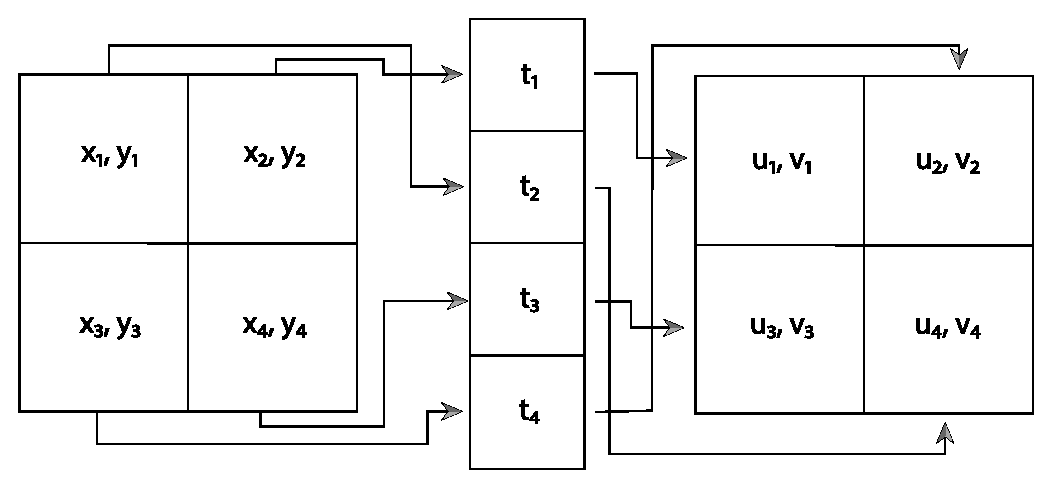
\includegraphics[width=0.8\linewidth]{chap07/Samplepadding.eps}
    \caption{我们可以生成良好的样本模式并获得分层的好处而不要求
        同时对所有采样维度分层。这里,我们已把$(x,y)$图像位置、
        时间$t$以及$(u,v)$透镜位置分为独立的层,每个都有四个区域。
        每个都是独立采样的,然后每个图像样本都随机关联一个时间样本
        和一个透镜样本。我们保留了在每个单独维度上分层的好处而不用指数级地增加样本总量。}
    \label{fig:7.16}
\end{figure}

\reffig{7.17}展示了在渲染景深时使用分层的透镜样本和
使用不分层的随机样本相比图像质量的提升。
\begin{figure}[htbp]
    \subfloat[参考]{\includegraphics[width=0.49\linewidth]{chap07/dof-ref.png}\label{fig:7.17.1}}\,
    \subfloat[随机采样]{\includegraphics[width=0.49\linewidth]{chap07/dof-random.png}\label{fig:7.17.2}}\\
    \subfloat[分层采样]{\includegraphics[width=0.49\linewidth]{chap07/dof-stratified.png}\label{fig:7.17.3}}
    \caption{渲染有景深的紫色球体时采样模式的影响。
        (a)模糊球体的高质量参考图像。(b)在每个像素中随机采样而无分层所生成的图像。
        (c)用同样数量的样本生成的图像,但用的是\refvar{StratifiedSampler}{},
        它分层了图像样本以及对该图更重要的透镜样本。对于该情形分层法做出了很大改善。}
    \label{fig:7.17}
\end{figure}

\reffig{7.18}展示比较了几种采样模式。
第一种是完全随机的模式:我们生成大量样本而完全不使用分层。
其结果很差;一些区域只有几个样本而另一些区域有好几团样本。
第二种是均匀分层模式。最后,均匀模式被扰动,
随机偏移量被加到每个样本的位置上,但仍将其保留在格子中。
这给出了比纯随机模式更好的整体分布而又保留了分层的好处,
尽管仍有一些样本团以及欠采样的区域。
\begin{figure}[htbp]
    \subfloat[]{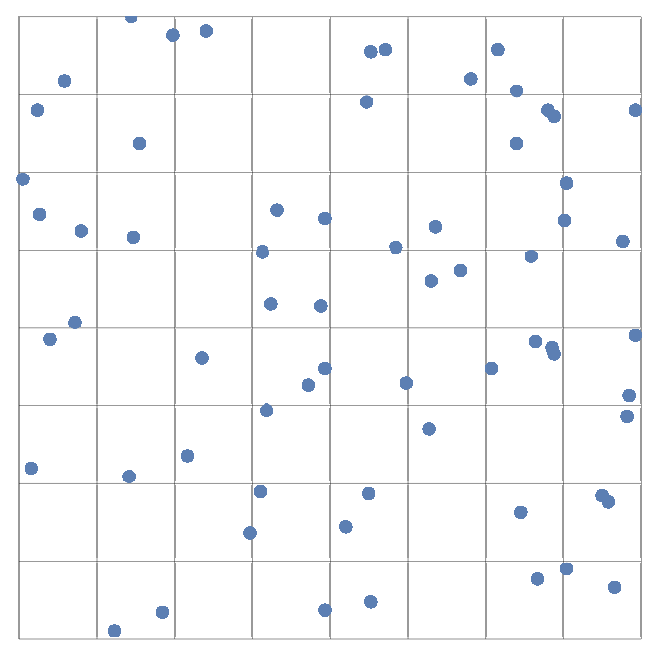
\includegraphics[width=0.49\linewidth]{chap07/random-point-samples.eps}\label{fig:7.18.1}}\,
    \subfloat[]{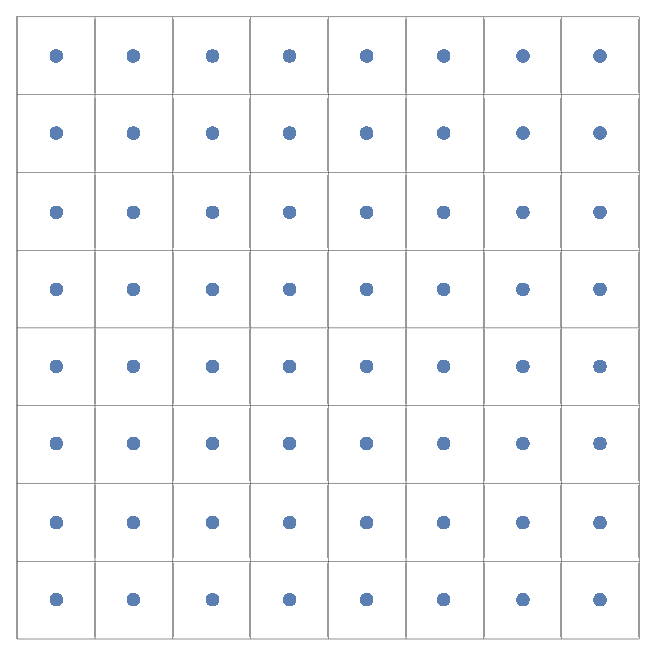
\includegraphics[width=0.49\linewidth]{chap07/uniform-point-samples.eps}\label{fig:7.18.2}}\\
    \subfloat[]{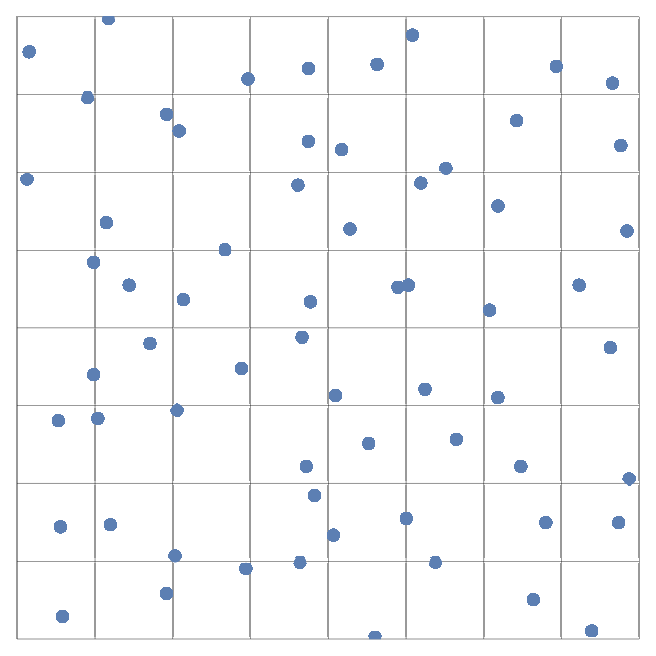
\includegraphics[width=0.49\linewidth]{chap07/jittered-point-samples.eps}\label{fig:7.18.3}}
    \caption{三种2D采样模式。(a)随机模式是无效模式,许多样本团让大片图像没有好好采样。
        (b)均匀分层模式的分布更好但会加剧混叠伪影。
        (c)分层扰动模式将来自均匀模式的混叠转化为高频噪声而仍保留了分层的好处。}
    \label{fig:7.18}
\end{figure}

\reffig{7.19}展示了用\refvar{StratifiedSampler}{}渲染的图像,
并展示了扰动的样本位置怎样将混叠伪影转化为不那么讨厌的噪声。
\begin{figure}[htbp]
    \centering
    \subfloat[参考]{\includegraphics[width=0.8\linewidth]{chap07/checkerboard-ref.png}\label{fig:7.19.1}}\\
    \subfloat[1个均匀样本]{\includegraphics[width=0.8\linewidth]{chap07/checkerboard-unif-1spp.png}\label{fig:7.19.2}}\\
    \subfloat[1个扰动样本]{\includegraphics[width=0.8\linewidth]{chap07/checkerboard-jitter-1spp.png}\label{fig:7.19.3}}\\
    \subfloat[4个扰动样本]{\includegraphics[width=0.8\linewidth]{chap07/checkerboard-jitter-4spp.png}\label{fig:7.19.4}}
    \caption{用棋盘纹理比较图像采样方法。这是幅很难渲染好的图像,
        因为当我们接近地平线时棋盘格关于像素间隔的频率趋于无穷。
        (a)参考图像,每个像素用256个样本渲染,展示了接近理想结果的样子。
        (b)每个像素只用一个样本渲染的图像,没有扰动。注意前景中格子边缘的锯齿伪影。
        还注意棋盘格函数在样本之间经历了许多周期的距离处的伪影;
        如之前介绍过的信号处理理论所料,细节错误地重复表现为低频混叠。
        (c)扰动图像样本的结果,每个像素还是只有一个样本。
        第二幅图像规则的混叠已经被替换为不那么讨厌的噪声伪影。
        (d)每个像素用四个扰动样本的结果仍然不如参考图像,但明显优于之前的结果。}
    \label{fig:7.19}
\end{figure}

\begin{lstlisting}
`\initcode{StratifiedSampler Declarations}{=}`
class `\initvar{StratifiedSampler}{}` : public `\refvar{PixelSampler}{}` {
public:
    `\refcode{StratifiedSampler Public Methods}{}`
private:
    `\refcode{StratifiedSampler Private Data}{}`
};
\end{lstlisting}
\begin{lstlisting}
`\initcode{StratifiedSampler Public Methods}{=}`
`\refvar{StratifiedSampler}{}`(int xPixelSamples, int yPixelSamples,
        bool jitterSamples, int nSampledDimensions)
    : `\refvar{PixelSampler}{}`(xPixelSamples * yPixelSamples, nSampledDimensions),
      `\refvar{xPixelSamples}{}`(xPixelSamples), `\refvar{yPixelSamples}{}`(yPixelSamples),
      `\refvar{jitterSamples}{}`(jitterSamples) { }
\end{lstlisting}
\begin{lstlisting}
`\initcode{StratifiedSampler Private Data}{=}`
const int `\initvar{xPixelSamples}{}`, `\initvar{yPixelSamples}{}`;
const bool `\initvar{jitterSamples}{}`;
\end{lstlisting}

作为\refvar{PixelSampler}{}的子类,
\refvar[StratifiedSampler::StartPixel]{StartPixel}{()}的实现必须按照传给\refvar{PixelSampler}{}
构造函数的维数{\ttfamily nSampledDimensions}一起生成1D和2D样本以及请求的数组样本。
\begin{lstlisting}
`\initcode{StratifiedSampler Method Definitions}{=}`
void `\refvar{StratifiedSampler}{}`::`\initvar[StratifiedSampler::StartPixel]{StartPixel}{}`(const `\refvar{Point2i}{}` &p) {
    `\refcode{Generate single stratified samples for the pixel}{}`
    `\refcode{Generate arrays of stratified samples for the pixel}{}`
    `\refvar{PixelSampler}{}`::StartPixel(p);
}
\end{lstlisting}

生成初始的分层样本后,它们被随机打乱;这是本节开头描述的填充方法。
如果没有进行打乱,则样本维度的值可能以某种方式相关而引发图像中的错误——
例如,用于选择胶片位置的首个2D样本和首个2D透镜样本会总是都在相邻于原点的左下方那层。
\begin{lstlisting}
`\initcode{Generate single stratified samples for the pixel}{=}`
for (size_t i = 0; i < `\refvar{samples1D}{}`.size(); ++i) {
    `\refvar{StratifiedSample1D}{}`(&`\refvar{samples1D}{}`[i][0], `\refvar{xPixelSamples}{}` * `\refvar{yPixelSamples}{}`,
                       `\refvar[PixelSampler::rng]{rng}{}`, `\refvar{jitterSamples}{}`);
    `\refvar{Shuffle}{}`(&`\refvar{samples1D}{}`[i][0], `\refvar{xPixelSamples}{}` * `\refvar{yPixelSamples}{}`, 1, `\refvar[PixelSampler::rng]{rng}{}`);
}
for (size_t i = 0; i < `\refvar{samples2D}{}`.size(); ++i) {
    `\refvar{StratifiedSample2D}{}`(&`\refvar{samples2D}{}`[i][0], `\refvar{xPixelSamples}{}`, `\refvar{yPixelSamples}{}`,
                       `\refvar[PixelSampler::rng]{rng}{}`, `\refvar{jitterSamples}{}`);
    `\refvar{Shuffle}{}`(&`\refvar{samples2D}{}`[i][0], `\refvar{xPixelSamples}{}` * `\refvar{yPixelSamples}{}`, 1, `\refvar[PixelSampler::rng]{rng}{}`);
}
\end{lstlisting}

1D和2D分层采样例程实现为实用函数。
两个都在域中给定层数上循环并在每个里面放置一个样本点。
\begin{lstlisting}
`\initcode{Sampling Function Definitions}{=}\initnext{SamplingFunctionDefinitions}`
void `\initvar{StratifiedSample1D}{}`(`\refvar{Float}{}` *samp, int nSamples, `\refvar{RNG}{}` &rng,
        bool jitter) {
    `\refvar{Float}{}` invNSamples = (`\refvar{Float}{}`)1 / nSamples;
    for (int i = 0; i < nSamples; ++i) {
        `\refvar{Float}{}` delta = jitter ? rng.`\refvar{UniformFloat}{}`() : 0.5f;
        samp[i] = std::min((i + delta) * invNSamples, `\refvar{OneMinusEpsilon}{}`);
    }
}
\end{lstlisting}

\refvar{StratifiedSample2D}{()}同样生成范围$[0,1)^2$中的样本。
\begin{lstlisting}
`\refcode{Sampling Function Definitions}{+=}\lastnext{SamplingFunctionDefinitions}`
void `\initvar{StratifiedSample2D}{}`(`\refvar{Point2f}{}` *samp, int nx, int ny, `\refvar{RNG}{}` &rng,
        bool jitter) {
    `\refvar{Float}{}` dx = (`\refvar{Float}{}`)1 / nx, dy = (`\refvar{Float}{}`)1 / ny;
    for (int y = 0; y < ny; ++y)
        for (int x = 0; x < nx; ++x) {
            `\refvar{Float}{}` jx = jitter ? rng.`\refvar{UniformFloat}{}`() : 0.5f;
            `\refvar{Float}{}` jy = jitter ? rng.`\refvar{UniformFloat}{}`() : 0.5f;
            samp->x = std::min((x + jx) * dx, `\refvar{OneMinusEpsilon}{}`);
            samp->y = std::min((y + jy) * dy, `\refvar{OneMinusEpsilon}{}`);
            ++samp;
        }
}
\end{lstlisting}

函数\refvar{Shuffle}{()}随机重排含有{\ttfamily count}个样本值的数组,
每个都有{\ttfamily nDimensions}维(换句话说,
尺寸为{\ttfamily nDimensions}的值构成的块被重排)。
\begin{lstlisting}
`\initcode{Sampling Inline Functions}{=}\initnext{SamplingInlineFunctions}`
template <typename T>
void `\initvar{Shuffle}{}`(T *samp, int count, int nDimensions, `\refvar{RNG}{}` &rng) {
    for (int i = 0; i < count; ++i) {
        int other = i + rng.`\refvar{UniformUInt32}{}`(count - i);
        for (int j = 0; j < nDimensions; ++j)
            std::swap(samp[nDimensions * i + j],
                      samp[nDimensions * other + j]);
    }
}
\end{lstlisting}

样本数组给我们出了个难题:例如若一个积分器
为像素中的每个样本请求样本向量中含64个2D样本值的数组,
则采样器有两个不同的目标要达成:
\begin{enumerate}
    \item 希望数组内的样本本身在2D上分布良好(例如通过使用$8\times8$分层网格)。
          这里的分层法会为每个单独的样本向量提升算出的结果的质量。
    \item 最好保证一个图像样本的数组中的每个样本都不要和图像中相邻样本的任何样本值太相似。
          即我们更希望点相对于其邻居能分布良好,使得在单个像素周围区域上就能很好覆盖整个样本空间。
\end{enumerate}

比起尝试同时解决这里的两个问题,\refvar{StratifiedSampler}{}只解决第一个。
本章后面的其他采样器会以更加精巧的技术回顾该问题并在不同程度上同时解决它们。

第二个复杂性来自于调用者可能会为每个图像样本请求任意数量样本的事实,
所以可能不易应用分层法。(例如,我们要怎么生成七个样本的分层2D模式?)
我们只能生成一个$n\times1$或$1\times n$的分层模式,
但这只能给我们在一个维度上分层的好处但不保证其他维度有好的模式。
方法{\ttfamily StratifiedSampler::RoundSize()}可以将请求进位到
下一个平方数,但我们将换用一种称为\keyindex{拉丁超立方采样}{Latin hypercube sampling}{}(LHS)的方法,
它能生成具有相当好分布的任意数量的任意维数样本。

LHS把每个维度轴均匀划分为$n$个区域并沿对角线在$n$个区域中的
每一个内生成一个扰动的样本,如\reffig{7.20}左边所示。
然后这些样本在每个维度上被随机打乱,生成分布良好的模式。
\begin{figure}[htbp]
    \centering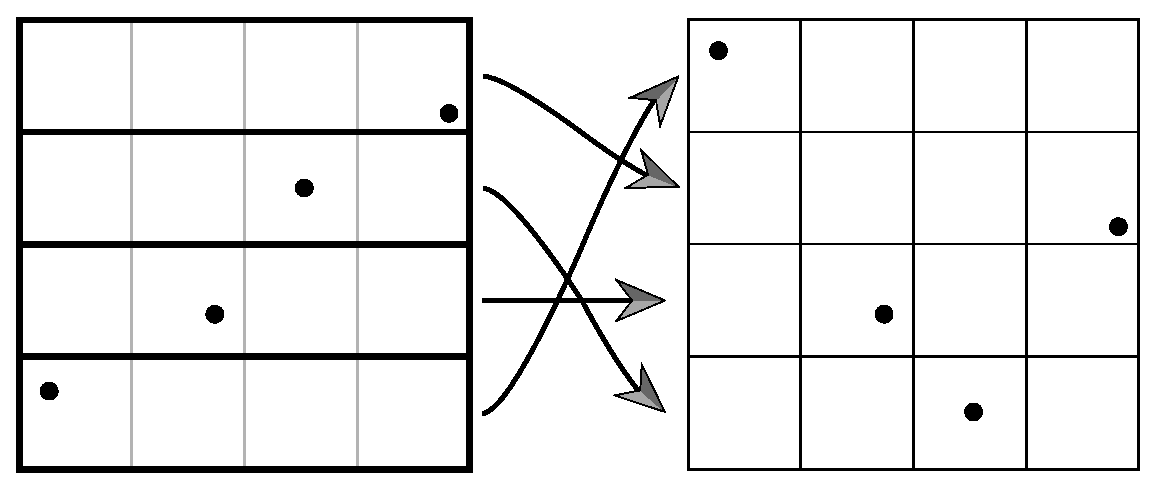
\includegraphics[width=0.8\linewidth]{chap07/LHSshuffle.eps}
    \caption{拉丁超立方采样(有时称为\protect\keyindex{$n$车采样}{$n$-rooks sampling}{})
        选择样本使得网格每行每列只出现单个样本。通过在对角线格子里生成随机样本
        然后随机重排它们的坐标可以做到这点。LHS的一个优点是它能像用分层模式那样
        生成具有良好分布的任意数量的样本,而不仅仅是$m\times n$个样本。}
    \label{fig:7.20}
\end{figure}

LHS的一个优点是当样本投影到样本维度的任意轴时它最小化了样本的聚集。
该性质与分层采样相反,后者2D模式中$n\times n$个样本里的$2n$个可能投影到每个轴上基本相同的点。
\reffig{7.21}展示了对于分层采样模式的这一最坏情况。
\begin{figure}[htbp]
    \centering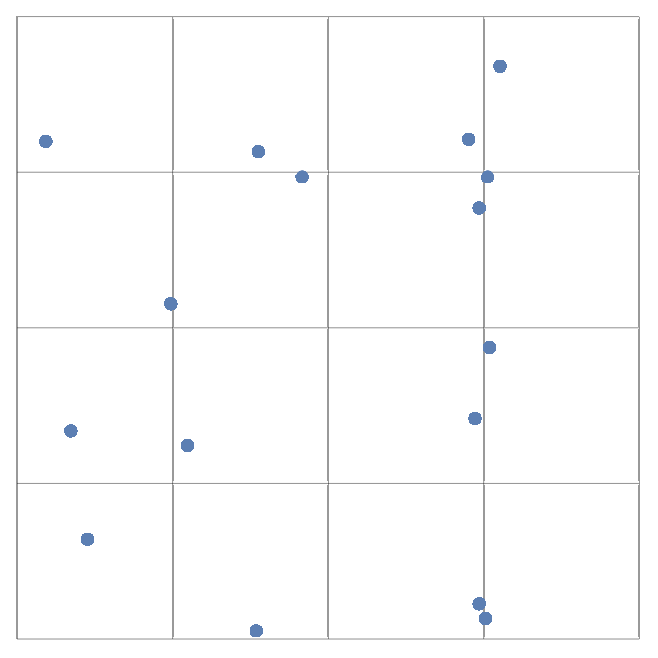
\includegraphics[width=0.4\linewidth]{chap07/stratified-bad-luck.eps}
    \caption{分层采样的一个最坏情况。在$n\times n$的2D模式中,
        多达$2n$个点可能投影到一个轴上基本相同的点。当生成像这样的“倒霉”模式时,
        用其算出的结果质量通常堪忧(这里,8个样本有几乎一样的$x$值)。}
    \label{fig:7.21}
\end{figure}

尽管解决了聚集问题,LHS对于分层采样并不是必要的改进;
很容易构造样本位置基本共线且大面积采样域没有相邻样本的情形
(例如原始样本的排列一致的时候,即让它们都保持原样)。
特别地,随着$n$增加,拉丁超立方模式比起分层模式越来越低效
\footnote{后续章节我们将回顾该问题,讨论同时是分层的且按拉丁超立方模式分布的样本模式。}。

通用的函数\refvar{LatinHypercube}{()}在任意维度生成任意数量的LHS样本。
因此数组{\ttfamily samples}中的元素数量应为{\ttfamily nSamples*nDim}。

\begin{lstlisting}
`\refcode{Sampling Function Definitions}{+=}\lastnext{SamplingFunctionDefinitions}`
void `\initvar{LatinHypercube}{}`(`\refvar{Float}{}` *samples, int nSamples, int nDim, `\refvar{RNG}{}` &rng) {
    `\refcode{Generate LHS samples along diagonal}{}`
    `\refcode{Permute LHS samples in each dimension}{}`
}
\end{lstlisting}
\begin{lstlisting}
`\initcode{Generate LHS samples along diagonal}{=}`
`\refvar{Float}{}` invNSamples = (`\refvar{Float}{}`)1 / nSamples;
for (int i = 0; i < nSamples; ++i)
    for (int j = 0; j < nDim; ++j) {
        `\refvar{Float}{}` sj = (i + (rng.`\refvar{UniformFloat}{}`())) * invNSamples;
        samples[nDim * i + j] = std::min(sj, `\refvar{OneMinusEpsilon}{}`);
    }
\end{lstlisting}

为了进行重排,该函数在样本上循环,每次在一个维度上随机重排样本点。
注意这和之前的\refvar{Shuffle}{()}例程是不一样的重排:
后者例程做一次重排,每个样本里的全部{\ttfamily nDim}个样本点是保持在一起的,
而这里是{\ttfamily nDim}次对单个维度的依次单独重排(\reffig{7.22})
\footnote{尽管不需要重排LHS模式的第一维,但这里的实现还是这样做了,
    因为让第一维的元素变为随机顺序意味着LHS模式可以与来自其他源的采样模式
    结合使用而没有其样本点间存在相关性的危险。}。
\begin{figure}[htbp]
    \centering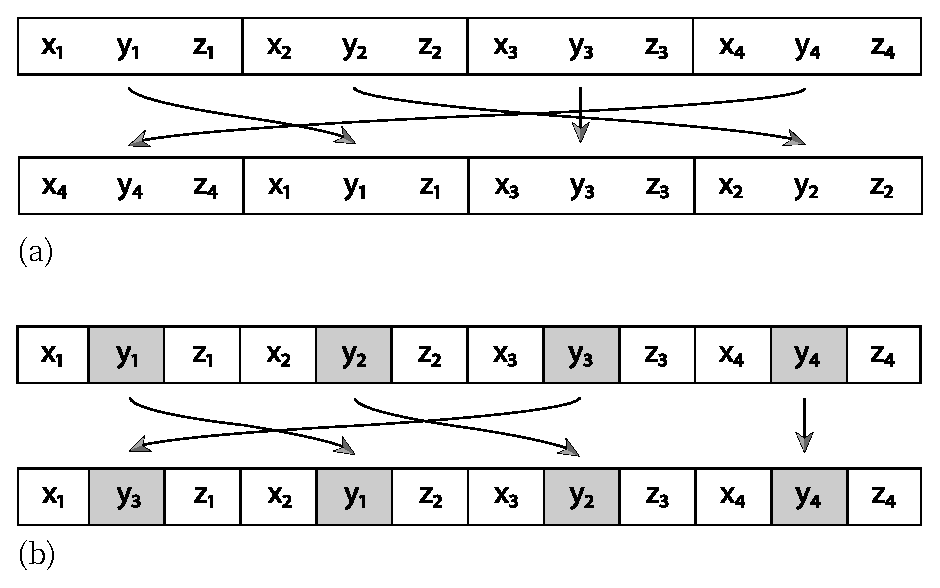
\includegraphics[width=0.8\linewidth]{chap07/Shufflepermutations.eps}
    \caption{(a)\refvar{Shuffle}{()}例程进行的重排移动附近的整块元素。
        (b)拉丁超立方采样的重排独立地排列每个维度的样本。
        这里展示了打乱四个三维元素模式的第二维样本。}
    \label{fig:7.22}
\end{figure}

\begin{lstlisting}
`\initcode{Permute LHS samples in each dimension}{=}`
for (int i = 0; i < nDim; ++i) {
    for (int j = 0; j < nSamples; ++j) {
        int other = j + rng.`\refvar{UniformUInt32}{}`(nSamples - j);
        std::swap(samples[nDim * j + i], samples[nDim * other + i]);
    }
}
\end{lstlisting}

有了函数\refvar{LatinHypercube}{()},
我们现在可以编写代码为当前像素计算样本数组了。
1D样本被分层然后随机打乱,而2D样本用拉丁超立方采样生成。
\begin{lstlisting}
`\initcode{Generate arrays of stratified samples for the pixel}{=}`
for (size_t i = 0; i < `\refvar{samples1DArraySizes}{}`.size(); ++i)
    for (int64_t j = 0; j < `\refvar{samplesPerPixel}{}`; ++j) {
        int count = `\refvar{samples1DArraySizes}{}`[i];
        `\refvar{StratifiedSample1D}{}`(&`\refvar{sampleArray1D}{}`[i][j * count], count, `\refvar[PixelSampler::rng]{rng}{}`,
                           `\refvar{jitterSamples}{}`);
        `\refvar{Shuffle}{}`(&`\refvar{sampleArray1D}{}`[i][j * count], count, 1, `\refvar[PixelSampler::rng]{rng}{}`);
    }
for (size_t i = 0; i < `\refvar{samples2DArraySizes}{}`.size(); ++i)
    for (int64_t j = 0; j < `\refvar{samplesPerPixel}{}`; ++j) {
        int count = `\refvar{samples2DArraySizes}{}`[i];
        `\refvar{LatinHypercube}{}`(&`\refvar{sampleArray2D}{}`[i][j * count].x, count, 2, `\refvar[PixelSampler::rng]{rng}{}`);
    }
\end{lstlisting}

我们将用\reffig{7.23}中的场景来阐述一些\refvar{Sampler}{}实现的性质。
\begin{figure}[htbp]
    \centering\includegraphics[width=0.75\linewidth]{chap07/area-light-example.png}
    \caption{面光源采样示例场景。}
    \label{fig:7.23}
\end{figure}

\reffig{7.24}展示了对于\refvar{DirectLightingIntegrator}{}而言来自好样本的提升。
第一幅图像每个像素用1个图像样本算得,每个有16个阴影样本。
第二幅每个像素用16个图像样本,每个有1个阴影样本。
因为\refvar{StratifiedSampler}{}能为第一种情况生成良好的LHS模式,
所以即使在取用的阴影样本总数相同时,其阴影质量也好得多。

\begin{figure}[htbp]
    \centering
    \subfloat[1个图像样本,16个阴影样本]{\includegraphics[width=\linewidth]{chap07/shadow-1-16.png}\label{fig:7.24.1}}\\
    \subfloat[16个图像样本,1个阴影样本]{\includegraphics[width=\linewidth]{chap07/shadow-16-1.png}\label{fig:7.24.2}}
    \caption{用来自分层采样器的样本采样面光源。
        (a)展示了每个像素用1个图像样本和16个阴影样本的结果,
        而(b)展示了用16个图像样本且每个只有1个阴影样本的结果。
        两种情况阴影样本的总数是一样的,但因为每个图像样本用16个阴影样本的版本
        可以使用LHS模式,像素区域内所有阴影样本都良好分布,而第二幅图像里
        这里的实现没有办法防止它们分布得很差。差别是惊人的。}
    \label{fig:7.24}
\end{figure}

\section{Halton采样器}\label{sec:Halton采样器}

\subsection{Hammersley和Halton序列}\label{sub:Hammersley和Halton序列}
\begin{lstlisting}
`\initcode{Low Discrepancy Function Definitions}{=}\initnext{LowDiscrepancyFunctionDefinitions}`
`\refvar{Float}{}` `\initvar{RadicalInverse}{}`(int baseIndex, uint64_t a) {
    switch (baseIndex) {
        case 0:
            `\refcode{Compute base-2 radical inverse}{}`
        case 1: return `\refvar{RadicalInverseSpecialized}{}`<3>(a);
        case 2: return `\refvar{RadicalInverseSpecialized}{}`<5>(a);
        case 3: return `\refvar{RadicalInverseSpecialized}{}`<7>(a);
        `\refcode{Remainder of cases for RadicalInverse()}{}`
    }
}
\end{lstlisting}

\section{(0,2)序列采样器}\label{sec:(0,2)序列采样器}
\begin{remark}
    本节含有高级内容,第一次阅读时可以跳过。
\end{remark}

另一个生成高质量样本的方法是利用某些低偏差序列的显著性质
即允许我们满足两个想要的样本性质(其中仅一个用\refvar{StratifiedSampler}{}满足了):
它们为图像样本的一个像素值生成样本向量使得每个像素样本的样本值都彼此间分布良好,
同时该像素中所有像素样本的样本值集合也整体上分布良好。

该序列使用Sobol\footnote{\protect\refsec{Sobol采样器}的\refvar{SobolSampler}{}使用了
    Sobol序列的所有维度。}推导出的低偏差序列的前两维。
该序列是一种特殊类型的低偏差序列,称为$(0,2)$序列。
$(0,2)$序列以非常常规的方式分层。例如,$(0,2)$序列中的前16个样本
满足来自\refsec{分层采样}中分层采样的分层约束,
意味着每个范围为$\displaystyle\left(\frac{1}{4},\frac{1}{4}\right)$的矩形中只存在一个样本。
然而它们还满足拉丁超立方约束,即在每个范围为$\displaystyle\left(\frac{1}{16},1\right)$和
$\displaystyle\left(1,\frac{1}{16}\right)$的矩形中只有一个样本。
此外,在每个范围为$\displaystyle\left(\frac{1}{2},\frac{1}{8}\right)$和
$\displaystyle\left(\frac{1}{8},\frac{1}{2}\right)$的矩形中只有一个样本。

\reffig{7.28}展示了划分域的所有可能,其中$(0,2)$序列前16个样本都满足分层性质。
从该模式中获取的每组含16个样本的后续序列也都满足这些分布性质。
\begin{figure}[htbp]
    \centering
    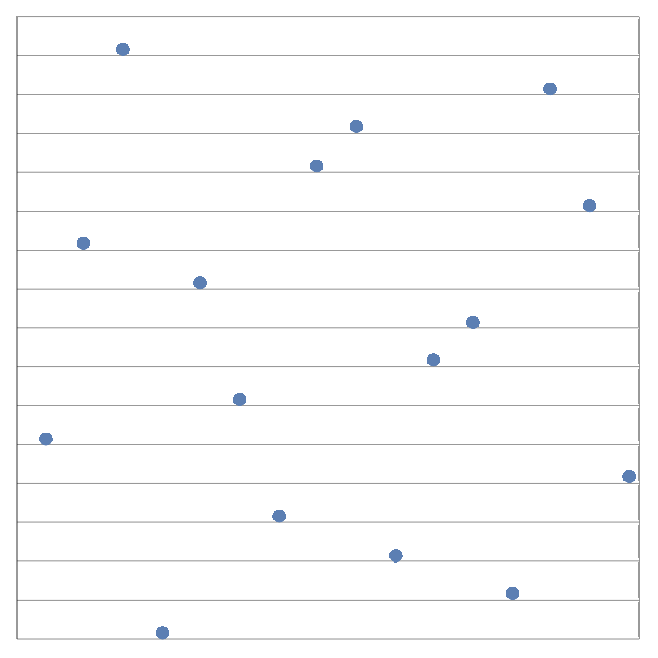
\includegraphics[width=0.49\linewidth]{chap07/elementary1x16.eps}\,
    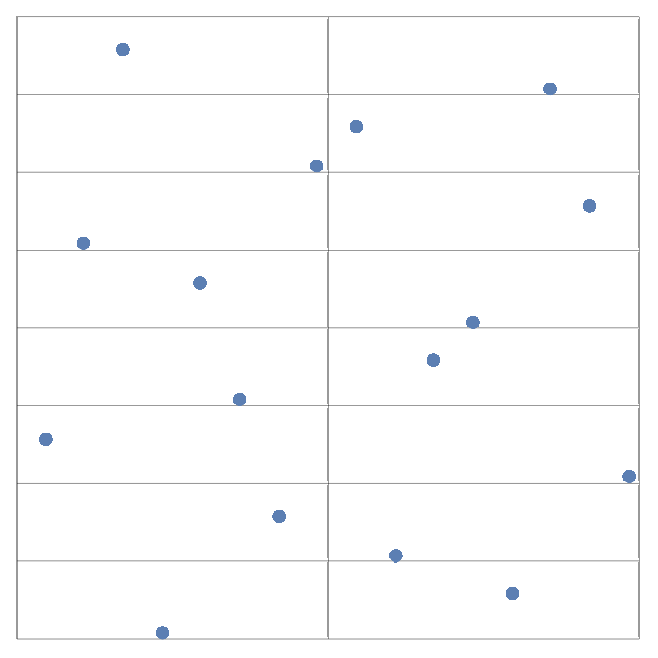
\includegraphics[width=0.49\linewidth]{chap07/elementary2x8.eps}\\
    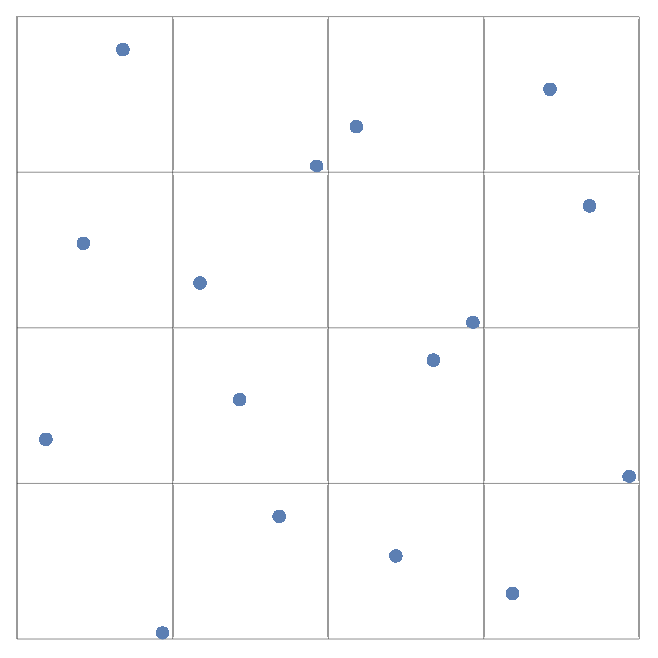
\includegraphics[width=0.49\linewidth]{chap07/elementary4x4.eps}\,
    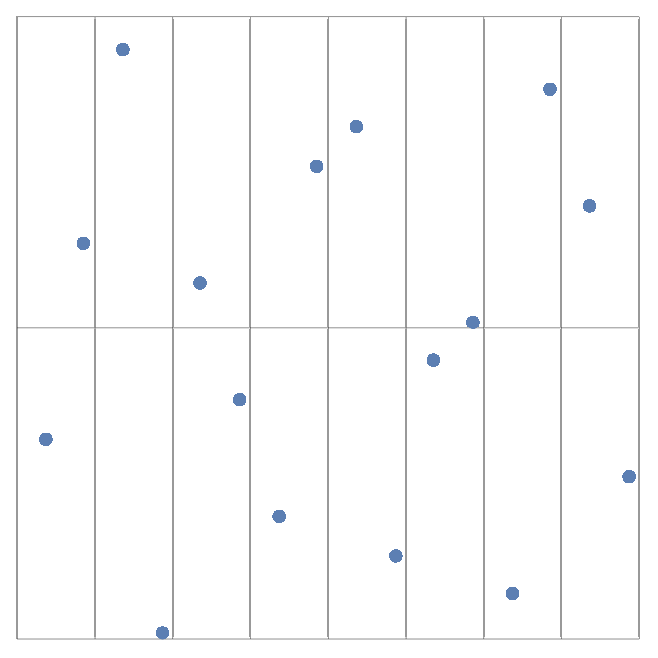
\includegraphics[width=0.49\linewidth]{chap07/elementary8x2.eps}\\
    \includegraphics[width=0.49\linewidth]{chap07/elementary16x1.eps}
    \caption{在所有以2为底数的基本区间中都只有单个样本的采样模式。
        它同时满足$4\times4$分层和拉丁超立方约束以及所示的其他两个分层约束。}
    \label{fig:7.28}
\end{figure}

通常任何来自$(0,2)$序列的长为$2^{l_1+l_2}$的序列(其中$l_i$为非负整数)
都满足该一般分层约束。以2为底的两维的\keyindex{基本区间}{elementary interval}{}定义为
\begin{align*}
    E=\left\{\left[\frac{a_1}{2^{l_1}},\frac{a_1+1}{2^{l_1}}\right)\times\left[\frac{a_2}{2^{l_2}},\frac{a_2+1}{2^{l_2}}\right)\right\}\, ,
\end{align*}
其中整数$a_i=0,1,2\ldots,2^{l_i}-1$.
该序列中前$2^{l_1+l_2}$个值中的每一个样本都在相应基本区间中。
此外,后续每$2^{l_1+l_2}$个值构成的集合也满足同样的性质。

现在为了理解怎样把$(0,2)$序列应用于生成2D样本,
考虑有$2\times2$图像样本的像素,每个含$4\times4$个2D样本构成的数组。
依据相应的基本区间集,$(0,2)$序列前$(2\times2)\times(4\times4)=2^6$个值相互之间分布良好。
此外依据其相应的基本区间,前$4\times4=2^4$个样本自己也分布良好,
其后的$2^4$个也是这样,以此类推。因此,我们可以为一个像素的
首个图像样本的$4\times4$数组样本使用前16个$(0,2)$序列样本,
然后下一个图像样本用接下来的16个,以此类推。
结果是分布非常良好的样本点集。

\subsection{用生成器矩阵采样}\label{sub:用生成器矩阵采样}
比起\refvar{HaltonSampler}{},Sobol序列基于不同的样本点生成机制,
它在各维度上使用了倒根。即使将倒根函数中的整数除法转化为乘法和位移,
高质量高分辨率渲染所需的计算数十亿样本的计算量也会很大。
大部分计算开销来自于在天生是2进制的计算机上执行不以2为底的计算
(考虑代码片\refcode{Compute base-2 radical inverse}{}和模板函数\refvar{RadicalInverseSpecialized}{()}间的差别)。


\section{最大化最小距离采样器}\label{sec:最大化最小距离采样器}


\section{Sobol采样器}\label{sec:Sobol采样器}
\begin{remark}
    本节含有高级内容,第一次阅读时可以跳过。
\end{remark}

本章最后一个\refvar{Sampler}{}基于一系列Sobol确定的生成矩阵。
来自这些矩阵生成的序列样本的区别在于能非常高效地实现——
因为是完全基于2进制计算的——而且在样本向量的全部$n$个维度上都分布得极好。
\reffig{7.34}展示了前几个Sobol生成矩阵。
\begin{figure}[htbp]
    \centering
    \includegraphics[width=0.24\linewidth]{chap07/sobol0.png}\,
    \includegraphics[width=0.24\linewidth]{chap07/sobol1.png}\,
    \includegraphics[width=0.24\linewidth]{chap07/sobol2.png}\,
    \includegraphics[width=0.24\linewidth]{chap07/sobol3.png}
    \caption{Sobol序列前四维的生成矩阵。注意其规则的结构。}
    \label{fig:7.34}
\end{figure}

\reffig{7.35}用景深测试场景比较了Sobol样本以及分层和Halton点。
\begin{figure}[htbp]
    \subfloat[分层采样]{\includegraphics[width=0.49\linewidth]{chap07/dof-stratified.png}\label{fig:7.35.1}}\,
    \subfloat[Halton采样]{\includegraphics[width=0.49\linewidth]{chap07/dof-halton.png}\label{fig:7.35.2}}\\
    \subfloat[Sobol采样]{\includegraphics[width=0.49\linewidth]{chap07/dof-sobol.png}\label{fig:7.35.3}}
    \caption{为渲染景深比较分层、Halton以及Sobol采样器。
        (a)用\refvar{StratifiedSampler}{}渲染的图像,
        (b)用\refvar{HaltonSampler}{}渲染的图像,以及
        (c)用\refvar{SobolSampler}{}渲染的图像。
        两个低偏差采样器都比分层采样器要好。尽管使用\refvar{SobolSampler}{}的该欠采样图像
        能看到结构化的网格伪影,但Sobol序列经常提供比Halton序列更快的收敛速度。}
    \label{fig:7.35}
\end{figure}

Sobol点的缺点是它们在收敛前容易出现结构化网格伪影;
在\reffig{7.36}展示的图像样本点中可以看出该问题。
\begin{figure}[htbp]
    \centering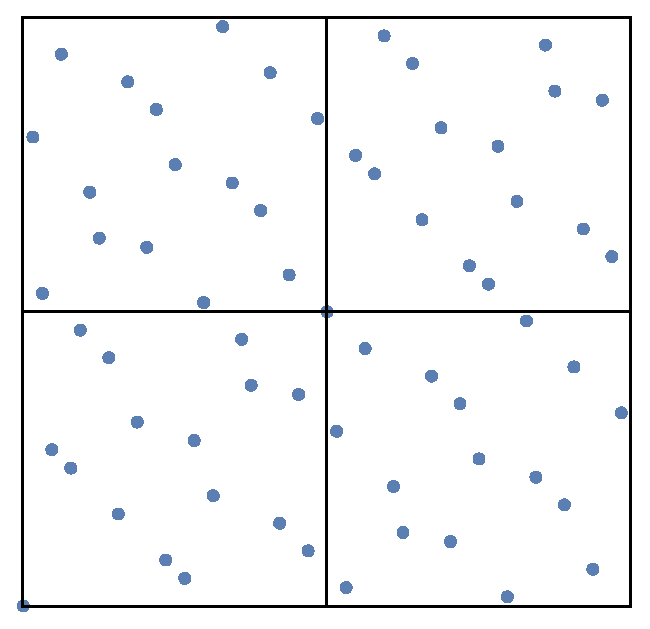
\includegraphics[width=0.5\linewidth]{chap07/sobol2x2pix.eps}
    \caption{$2\times2$像素的网格,每个用16个Sobol样本采样。
        注意有大量结构,且许多样本互相靠近。该序列在样本向量全部$n$个维度上
        极好的分布性质通常弥补了这些缺点。}
    \label{fig:7.36}
\end{figure}

在\reffig{7.37}的图像中该结构是可见的。
该缺点换来的是,Sobol序列在样本序列全部$n$个维度上分布得极其好。
\begin{figure}[htbp]
    \centering
    \subfloat[Halton采样器]{\includegraphics[width=\linewidth]{chap07/car-halton-undersampled.png}\label{fig:7.37.1}}\\
    \subfloat[Sobol采样器]{\includegraphics[width=\linewidth]{chap07/car-sobol-undersampled.png}\label{fig:7.37.2}}
    \caption{用(a)Halton采样器和(b)Sobol采样器渲染的欠采样图像。
        虽然具有不同的视觉特征,但两个都展现出可见的结构。
        特别是Sobol序列展现出清晰可见的棋盘结构。}
    \label{fig:7.37}
\end{figure}

\begin{lstlisting}
`\initcode{SobolSampler Declarations}{=}`
class `\initvar{SobolSampler}{}` : public `\refvar{GlobalSampler}{}` {
public:
    `\refcode{SobolSampler Public Methods}{}`
private:
    `\refcode{SobolSampler Private Data}{}`
};
\end{lstlisting}

\refvar{SobolSampler}{}用能让样本域$[0,1)^2$覆盖住要采样的图像区域
的最小幂2值来均匀缩放前两维。像\refvar{HaltonSampler}{}那样,
选择该特定缩放方案是为了让计算从像素坐标到每个像素内样本索引的逆映射更容易。
\begin{lstlisting}
`\initcode{SobolSampler Public Methods}{=}`
`\refvar{SobolSampler}{}`(int64_t samplesPerPixel, const `\refvar{Bounds2i}{}` &sampleBounds)
    : `\refvar{GlobalSampler}{}`(`\refvar{RoundUpPow2}{}`(samplesPerPixel)),
      `\refvar{sampleBounds}{}`(sampleBounds) {
    `\refvar{resolution}{}` = `\refvar{RoundUpPow2}{}`(std::max(sampleBounds.`\refvar{Diagonal}{}`().x,
                                      sampleBounds.`\refvar{Diagonal}{}`().y));
    `\refvar{log2Resolution}{}` = `\refvar{Log2Int}{}`(`\refvar{resolution}{}`);
}
\end{lstlisting}
\begin{lstlisting}
`\initcode{SobolSampler Private Data}{=}`
const `\refvar{Bounds2i}{}` `\initvar{sampleBounds}{}`;
int `\initvar{resolution}{}`, `\initvar{log2Resolution}{}`;
\end{lstlisting}

如果采样域$[0,1)^2$已被缩放$2^{\text{\ttfamily log2Resolution}}$倍
以覆盖像素采样区域,则函数\refvar{SobolIntervalToIndex}{()}返回
像素{\ttfamily p}内第{\ttfamily sampleNum}个样本的索引。
\begin{lstlisting}
`\refcode{Low Discrepancy Declarations}{+=}\lastcode{LowDiscrepancyDeclarations}`
inline uint64_t `\initvar{SobolIntervalToIndex}{}`(const uint32_t log2Resolution,
    uint64_t sampleNum, const `\refvar{Point2i}{}` &p);
\end{lstlisting}

用于推导它所实现的算法的一般方法和Halton采样器在其方法\linebreak
\refvar{GetIndexForSample}{()}中用的一样。
这里用幂2缩放意味着缩放值以2为底的对数给出了
构建缩放后样本整数部分的积${\bm C}[d_i(a)]^{\mathrm{T}}$的位数。
为了求得缩放后能给出特定整数值的$a$值,我们可以计算$\bm C$的逆:设
\begin{align*}
    v={\bm C}[d_i(a)]^{\mathrm{T}}\, ,
\end{align*}
则等价地
\begin{align*}
    {\bm C}^{-1}v=[d_i(a)]^{\mathrm{T}}\, .
\end{align*}
我们这里不会介绍该方法的实现。
\begin{lstlisting}
`\initcode{SobolSampler Method Definitions}{=}\initnext{SobolSamplerMethodDefinitions}`
int64_t `\refvar{SobolSampler}{}`::`\initvar[SobolSampler::GetIndexForSample]{\refvar{GetIndexForSample}{}}{}`(int64_t sampleNum) const {
    return `\refvar{SobolIntervalToIndex}{}`(`\refvar{log2Resolution}{}`, sampleNum,
        `\refvar{Point2i}{}`(`\refvar{currentPixel}{}` - `\refvar{sampleBounds}{}`.`\refvar{pMin}{}`));
}
\end{lstlisting}

\section{图像重构}\label{sec:图像重构}

\subsection{滤波器函数}\label{sub:滤波器函数}

\begin{lstlisting}
`\initcode{Filter Declarations}{=}`
class `\initvar{Filter}{}` {
public:
    `\refcode{Filter Interface}{}`
    `\refcode{Filter Public Data}{}`
};
\end{lstlisting}

{\noindent\hfil$=========$\hfil{\color{red}{施工分割线}}\hfil$=========$\
\section{胶片与成像管道}\label{sec:胶片与成像管道}

\subsection{胶片类}\label{sub:胶片类}

\begin{lstlisting}
`\initcode{Film Declarations}{=}\initnext{FilmDeclarations}`
class `\initvar{Film}{}` {
public:
    `\refcode{Film Public Methods}{}`
    `\refcode{Film Public Data}{}`
private:
    `\refcode{Film Private Data}{}`
    `\refcode{Film Private Methods}{}`
};
\end{lstlisting}

\begin{lstlisting}
`\initcode{Film Method Definitions}{=}\initnext{FilmMethodDefinitions}`
`\refvar{Film}{}`::`\refvar{Film}{}`(const `\refvar{Point2i}{}` &resolution, const `\refvar{Bounds2f}{}` &cropWindow,
        std::unique_ptr<`\refvar{Filter}{}`> filt, `\refvar{Float}{}` `\refvar{diagonal}{}`,
        const std::string &`\refvar{filename}{}`, `\refvar{Float}{}` `\refvar{scale}{}`)
    : `\refvar{fullResolution}{}`(resolution), `\refvar{diagonal}{}`(`\refvar{diagonal}{}` * .001),
    `\refvar{filter}{}`(std::move(filt)), `\refvar{filename}{}`(`\refvar{filename}{}`), `\refvar{scale}{}`(`\refvar{scale}{}`) {
    `\refcode{Compute film image bounds}{}`
    `\refcode{Allocate film image storage}{}`
    `\refcode{Precompute filter weight table}{}`
}
\end{lstlisting}

\begin{lstlisting}
`\initcode{Film Public Data}{=}\initnext{FilmPublicData}`
const `\refvar{Point2i}{}` `\initvar{fullResolution}{}`;
const `\refvar{Float}{}` `\initvar{diagonal}{}`;
std::unique_ptr<`\refvar{Filter}{}`> `\initvar{filter}{}`;
const std::string `\initvar{filename}{}`;
\end{lstlisting}

\begin{lstlisting}
`\initcode{Film Private Data}{=}\initnext{FilmPrivateData}`
struct `\initvar{Pixel}{}` {
    `\refvar{Float}{}` `\initvar[Pixel:xyz]{xyz}{}`[3] = { 0, 0, 0 };
    `\refvar{Float}{}` `\initvar[Pixel:filterWeightSum]{filterWeightSum}{}` = 0;
    `\refvar{AtomicFloat}{}` `\initvar[Pixel:splatXYZ]{splatXYZ}{}`[3];
    `\refvar{Float}{}` `\initvar[Pixel:pad]{pad}{}`;
};
std::unique_ptr<`\refvar{Pixel}{}`[]> `\initvar[Pixel::pixels]{pixels}{}`;
\end{lstlisting}

\begin{lstlisting}
`\refcode{Film Method Definitions}{+=}\lastnext{FilmMethodDefinitions}`
`\refvar{Bounds2i}{}` `\refvar{Film}{}`::`\initvar{GetSampleBounds}{()}` const {
    `\refvar{Bounds2f}{}` floatBounds(
        `\refvar{Floor}{}`(`\refvar{Point2f}{}`(croppedPixelBounds.pMin) + `\refvar{Vector2f}{}`(0.5f, 0.5f) -
              `\refvar{filter}{}`->`\refvar[Filter::radius]{radius}{}`),
        `\refvar{Ceil}{}`( `\refvar{Point2f}{}`(croppedPixelBounds.pMax) - `\refvar{Vector2f}{}`(0.5f, 0.5f) +
              `\refvar{filter}{}`->`\refvar[Filter::radius]{radius}{}`));
    return (`\refvar{Bounds2i}{}`)floatBounds;
}
\end{lstlisting}
\begin{lstlisting}
`\refcode{Film Method Definitions}{+=}\lastnext{FilmMethodDefinitions}`
`\refvar{Bounds2f}{}` `\refvar{Film}{}`::`\initvar{GetPhysicalExtent}{}`() const {
    `\refvar{Float}{}` aspect = (`\refvar{Float}{}`)`\refvar{fullResolution}{}`.y / (`\refvar{Float}{}`)`\refvar{fullResolution}{}`.x;
    `\refvar{Float}{}` x = std::sqrt(`\refvar{diagonal}{}` * `\refvar{diagonal}{}` / (1 + aspect * aspect));
    `\refvar{Float}{}` y = aspect * x;
    return `\refvar{Bounds2f}{}`(`\refvar{Point2f}{}`(-x / 2, -y / 2), `\refvar{Point2f}{}`(x / 2, y / 2));
}
\end{lstlisting}
\subsection{为胶片提供像素值}\label{sub:为胶片提供像素值}
\begin{lstlisting}
`\refcode{Film Method Definitions}{+=}\lastnext{FilmMethodDefinitions}`
std::unique_ptr<`\refvar{FilmTile}{}`> `\refvar{Film}{}`::`\initvar{GetFilmTile}{}`(
        const `\refvar{Bounds2i}{}` &sampleBounds) {
    `\refcode{Bound image pixels that samples in sampleBounds contribute to}{}`
    return std::unique_ptr<`\refvar{FilmTile}{}`>(new FilmTile(tilePixelBounds,
        filter->radius, filterTable, filterTableWidth));
}
\end{lstlisting}

\begin{lstlisting}
`\refcode{Film Declarations}{+=}\lastcode{FilmDeclarations}`
class `\initvar{FilmTile}{}` {
public:
    `\refcode{FilmTile Public Methods}{}`
private:
    `\refcode{FilmTile Private Data}{}`
};
\end{lstlisting}

\begin{lstlisting}
`\initcode{FilmTile Public Methods}{=}\initnext{FilmTilePublicMethods}`
`\refvar{FilmTile}{}`(const `\refvar{Bounds2i}{}` &pixelBounds, const `\refvar{Vector2f}{}` &filterRadius,
    const `\refvar{Float}{}` *filterTable, int filterTableSize)
    : `\refvar{pixelBounds}{}`(pixelBounds), `\refvar{filterRadius}{}`(filterRadius),
    `\refvar{invFilterRadius}{}`(1 / filterRadius.x, 1 / filterRadius.y),
    `\refvar{filterTable}{}`(filterTable), `\refvar{filterTableSize}{}`(filterTableSize) {
    `\refvar[FilmTile::pixels]{pixels}{}` = std::vector<`\refvar{FilmTilePixel}{}`>(std::max(0, pixelBounds.Area()));
}
\end{lstlisting}

\begin{lstlisting}
`\initcode{FilmTile Private Data}{=}`
const `\refvar{Bounds2i}{}` `\initvar{pixelBounds}{}`;
const `\refvar{Vector2f}{}` `\initvar{filterRadius}{}`, `\initvar{invFilterRadius}{}`;
const `\refvar{Float}{}` *`\initvar{filterTable}{}`;
const int `\initvar{filterTableSize}{}`;
std::vector<`\refvar{FilmTilePixel}{}`> `\initvar[FilmTile::pixels]{pixels}{}`;
\end{lstlisting}

\begin{lstlisting}
`\refcode{FilmTile Public Methods}{+=}\lastnext{FilmTilePublicMethods}`
void `\initvar{AddSample}{}`(const `\refvar{Point2f}{}` &pFilm, const `\refvar{Spectrum}{}` &L,
    `\refvar{Float}{}` sampleWeight = 1.) {
    `\refcode{Compute sample's raster bounds}{}`
    `\refcode{Loop over filter support and add sample to pixel arrays}{}`
}
\end{lstlisting}

\begin{lstlisting}
`\initcode{Compute sample's raster bounds}{=}`
`\refvar{Point2f}{}` pFilmDiscrete = pFilm - `\refvar{Vector2f}{}`(0.5f, 0.5f);
`\refvar{Point2i}{}` p0 = (`\refvar{Point2i}{}`)`\refvar{Ceil}{}`(pFilmDiscrete - filterRadius);
`\refvar{Point2i}{}` p1 = (`\refvar{Point2i}{}`)`\refvar{Floor}{}`(pFilmDiscrete + filterRadius) + `\refvar{Point2i}{}`(1, 1);
p0 = `\refvar[Point3::Max]{Max}{}`(p0, pixelBounds.pMin);
p1 = `\refvar[Point3::Min]{Min}{}`(p1, pixelBounds.pMax);
\end{lstlisting}

\begin{lstlisting}
`\refcode{Film Method Definitions}{+=}\lastnext{FilmMethodDefinitions}`
void `\refvar{Film}{}`::`\initvar{MergeFilmTile}{}`(std::unique_ptr<`\refvar{FilmTile}{}`> tile) {
    std::lock_guard<std::mutex> lock(`\refvar{mutex}{}`);
    for (`\refvar{Point2i}{}` pixel : tile->`\refvar{GetPixelBounds}{}`()) {
        `\refcode{Merge pixel into Film::pixels}{}`
    }
}
\end{lstlisting}
\begin{lstlisting}
`\refcode{Film Private Data}{+=}\lastnext{FilmPrivateData}`
std::mutex `\initvar{mutex}{}`;
\end{lstlisting}
\begin{lstlisting}
`\refcode{FilmTile Public Methods}{+=}\lastcode{FilmTilePublicMethods}`
`\refvar{Bounds2i}{}` `\initvar{GetPixelBounds}{}`() const { return `\refvar{pixelBounds}{}`; }
\end{lstlisting}
\begin{lstlisting}
`\refcode{Film Private Data}{+=}\lastcode{FilmPrivateData}`
const `\refvar{Float}{}` `\initvar{scale}{}`;
\end{lstlisting}

\subsection{图像输出}\label{sub:图像输出}
\begin{lstlisting}
`\refcode{Film Method Definitions}{+=}\lastcode{FilmMethodDefinitions}`
void `\refvar{Film}{}`::`\initvar[Film::WriteImage]{WriteImage}{}`(`\refvar{Float}{}` splatScale) {
    `\refcode{Convert image to RGB and compute final pixel values}{}`
    `\refcode{Write RGB image}{}`
}
\end{lstlisting}

\section{习题}\label{sec:习题07}
\begin{enumerate}
      \item \circletwo 可以根据\refvar{RadicalInverse}{()}中的实现代码,
            为基2实现一个专门版本的\refvar{ScrambledRadicalInverse}{()}。
            确定怎样将随机数字排列映射为单个数位运算并实现该方法。
            比较算出的值和当前实现生成的值以确保你的方法是对的
            并通过编写一个小巧的基准程序来度量你的方法有多快。
      \item \circletwo 当前,每个样本的第三到五维是被时间和镜头样本用掉的,
            即便并非所有场景都需要这些样本值。因为样本向量中的更低维常比
            后面的分布得更好,所以这会造成不必要的图像质量下降。
            修改pbrt使得相机能表明其样本需求然后在需要样本来
            初始化\refvar{CameraSample}{}时利用该信息。
            别忘了更新\refvar[arrayStartDim]{GlobalSampler::arrayStartDim}{}的值。
            用\refvar{DirectLightingIntegrator}{}
            渲染图像并和当前实现的结果比较。你看到有改进吗?
            用不同采样器时结果有何区别?你怎样解释你所见到的各采样器间的任何区别?
      \item \label{sub:7.11.3}\circletwo 把\citet{Kensler2013Pixar}介绍
            改进的多重扰动采样方法实现为pbrt中的新
            \refvar{Sampler}{}。比较它和用\refvar{StratifiedSampler}{}、
            \refvar{HaltonSampler}{}以及\refvar{SobolSampler}{}渲染时
            的图像质量和渲染时间。
      \item \circletwo\citet{10.1007/3-540-31186-6_14}\sidenote{译者注:
                  在Springer获取的引用条目标注为2006年,
                  属于2004年的会议;原文则均标为2004年。}
            和\citet{10.1007/978-3-540-74496-2_12}\sidenote{译者注:
                  在Springer获取的引用条目标注为2008年,属于2006年的会议;
                  原文则均标为2006年。}描述了图像合成中\keyindex{一阶点阵}{rank-1 lattices}{}的应用。
            一阶点阵是另一种高效生成高质量低偏差样本点序列的方式。
            阅读他们的论文并基于该方法实现一个\refvar{Sampler}{}。
            比较它和pbrt中其他采样器的结果。
      \item \circletwo 用pbrt当前的\refvar{FilmTile}{}实现时,
            若重新渲染一幅图像,由于线程在后续运行中以不同顺序完成图块,
            图像中的像素值可能有轻微变化。例如一个像素最终值取自三个不同
            图像采样块中的样本,$v_1+v_2+v_3$,其值可能有时算作$(v_1+v_2)+v_3$
            而有时为$v_1+(v_2+v_3)$.由于浮点舍入,这两个值可能不同。
            尽管这些区别通常不成问题,但当想用自动化测试脚本验证对系统
            作出的无伤大雅的更改不会在渲染图像中实际引发任何区别时,
            它们就会造成灾难。修改\refvar[MergeFilmTile]{Film::MergeFilmTile}{()}使其
            以一致的顺序合并图块,从而让最终像素值不再被该不一致性干扰
            (例如你的实现可能缓存\refvar{FilmTile}{}并只在一个图块的
            上方和左侧相邻图块都已被合并时才合并它)。确保你的实现不引入
            任何意义上的性能倒退。度量因\refvar{FilmTile}{}生命期更长
            而新增的内存使用量;它和总内存使用量有什么关系?
      \item \circletwo 如\refsec{胶片与成像管道}中所述,
            方法\refvar[AddSplat]{Film::AddSplat}{()}没用滤波函数
            而是代之高效地用矩形滤波器把样本溅射到其最靠近的单个像素上。
            为了应用任意滤波器,必须规范化滤波器使得它在定义域上的积分为一;
            pbrt目前并不要求\refvar{Filter}{}满足该约束。
            修改\refvar{Film}{}构造函数中\refvar[Film::filterTable]{filterTable}{}的计算,
            使得制表函数规范化(别忘了在计算规范化因子时,
            表格只保存函数四分之一的范围)。然后修改方法\refvar{AddSplat}{()}的
            实现以使用该滤波器。研究其导致的执行时间和图像质量的区别。
      \item \circleone 修改pbrt以创建为每条相机光线存于\refvar{Film}{}的值
            都正比于计算该光线辐亮度所花时长的图像(一个1像素宽的矩形滤波器
            可能是对该习题最有用的滤波器)。用该技术渲染各种场景。
            得到的图像对于系统性能带来了怎样的启发?当你查看它们时
            你可能需要缩放像素值或取其对数来看到有意义的变化。
      \item \circletwo 辐射度量学中线性假设的一个优点是场景的最终图像和
            分别考虑每个光源分布的图像之和是一样的(假设使用不会
            截断像素辐亮度值的浮点图像块格式)。该性质意味着如果渲染器为
            每个光源创建单独的图像,可以写个交互式灯光设计工具让
            快速查看缩放场景中单个光源作用的影响而无需重新渲染成为可能。
            可代之以缩放一个光源的单独图像然后再对所有光源图像求和
            重新生成最终图像(该技术首先应用于\citet{10.1145/122718.122723}的
            歌剧灯光设计)。修改pbrt来为场景中的每个光源输出单独的图像,
            并写一个按该方式利用它们的交互式灯光设计工具。
      \item \circlethree \citet{10.1145/54852.378514}注意到
            有一簇重建滤波器同时用了函数值和它在该点的导数来进行
            比只知道函数值好得多的重建。此外,他们报告他们已为朗伯和
            冯氏反射模型\sidenote{译者注:原文Lambertian and Phong reflection models。}的
            屏幕空间导数推导出解析解,然而他们没有在其论文中包含这些表达式。
            研究基于导数的重建,扩展pbrt以支持该技术。
            因为给一般形状和BSDF模型的屏幕空间导数推导表达式可能很难,
            研究基于有限差分的近似即可。\refsec{采样与抗锯齿}射线差分背后
            基于该思想的技术可能对该尝试有成效。
      \item \circlethree \keyindex{基于图像的渲染}{image-based rendering}{render渲染}是
            使用一个场景一幅或多幅图像合成不同于原始视角的新视角图像的一组技术的总称。
            其中一种方法是\keyindex{光场渲染}{light field rendering}{render渲染},
            即用一组来自密集间隔位置的图像\citep{10.1145/237170.237199,10.1145/237170.237200}。
            阅读这两篇关于光场的论文,并修改pbrt以直接生成场景的光场,
            而不需要渲染器运行多次,每次只针对一个相机位置。
            为此可能有必要编写专门的\refvar{Camera}{}、\refvar{Sampler}{}和\refvar{Film}{}。
            此外,编写一个交互式光场查看器来加载你的实现生成的光场并生成场景的新视角。
      \item \circlethree 比起只保存图像中的光谱值,常常更有用的是
            保存场景中在每个像素处可见的物体的额外信息。
            例如见\citet{10.1145/325334.325247}和\citet{10.1145/97879.97901}的SIGGRAPH论文。
            例如,如果保存每个像素处物体的3D位置、曲面法线以及BRDF,
            则移动光源后可高效地重新渲染场景\citep{10.1145/344779.344938}。
            或者,如果每个样本保存沿其相机光线可见的所有物体信息而不是只存第一个,
            则可以重新渲染移动视点后的新图像\citep{10.1145/280814.280882}。
            研究深帧缓冲区\sidenote{译者注:原文deep frame buffer,不确定该词翻译。}的表示
            和利用它的算法;扩展pbrt以支持创建像这样的图像,并开发对它们进行操作的工具。
      \item \circletwo 为图像重建实现中值滤波器:对于每个像素,保存
            滤波器范围内其周围所有样本的中值。该任务很复杂,因为事实上
            当前\refvar{Film}{}实现中的滤波器必须是\keyindex{线性的}{linear}{}——
            滤波函数值只取决于样本相对于像素位置的位置,样本值对滤波函数值没有影响。
            因为实现假设滤波器是线性的,且因为它在把样本值的贡献加到图像中后就不再保存了,
            所以实现中值滤波器要求一般化\refvar{Film}{}或开发新的\refvar{Film}{}实现。
            用像\refvar{PathIntegrator}{}那样搭配常规图像滤波器会有讨厌的图像噪声的积分器渲染图像。
            中值滤波器在减少噪声上有多成功?用中值滤波器有视觉缺陷吗?
            你能实现该方法而无需在计算最终像素值前保存所有图像样本值吗?
      \item \circletwo 中值滤波器的一种替代是丢弃像素滤波器区域中
            具有最小贡献的样本和具有最大贡献的样本。该方法更多使用采样期间收集的信息。
            实现该方法并比较它和中值滤波器的结果。
      \item \circlethree 实现\citeauthor{keller1998quasi}及其合作者
            介绍的非连续缓冲区\citep{keller1998quasi,10.2312:EGWR:EGWR02:015-024}。
            你可能需要修改\refvar{Integrator}{}的接口使得它们可以独自返回
            直接和间接照明贡献然后独立将其传给\refvar{Film}{}。
            渲染图像以展示其在用间接照明渲染图像时的高效性。
      \item \circlethree 实现近年一种自适应采样和重建技术,
            例如\citet{10.1145/1360612.1360632}、\citet{10.1145/1531326.1531399}、
            \citet{10.1145/1618452.1618486}或者\citet{10.1145/2641762}介绍的。
            比起只用高采样率的均匀采样它们生成同等质量图像要高效多少?
            对于无需自适应采样的简单场景它们如何影响运行时间?
      \item \circlethree 调研色调重建算法的当前研究
            (例如见\citet{reinhard2010high}、\citet{10.1145/2366145.2366220}),
            并实现其中一个或多个算法。对pbrt渲染的大量场景使用你的实现,
            并讨论比起查看无色调重建的图像你所见到的改进。
\end{enumerate}

\section{译者补充:信号处理}\label{sec:译者补充:信号处理}
\begin{remark}
    本节内容不是原书内容,而是译者根据\citet{enwiki:1115652231,enwiki:1115414995,
        enwiki:1098200554,enwiki:1114206769}、\citet{DigitalSignalProcessing}补充的,
    请酌情参考和斧正。
\end{remark}
\begin{notation}
    本节所指的时域和原书前文中的空域是等价的概念,不影响本质。
\end{notation}
\subsection{单位冲激函数}\label{sub:单位冲激函数}
\begin{definition}
    数学中,\keyindex{狄拉克$\delta$分布}{Dirac delta distribution}{}是定义在实数域上的广义分布或函数。
    它在除零以外的点上都取零,且在整个实数域上的积分等于一。通常记作$\delta(\cdot)$.
\end{definition}

狄拉克$\delta$分布也称\keyindex{狄拉克$\delta$函数}{Dirac delta function}{},
简称\keyindex{$\delta$分布}{delta distribution}{}或
\keyindex{$\delta$函数}{delta function}{},
它最早由英国理论物理学家保罗·狄拉克(Paul Adrien Maurice Dirac)提出,
在物理和工程界有广泛应用,也称作\keyindex{单位冲激函数}{unit impulse function}{}。

单位冲激函数不是严格意义上的函数,但形式上遵守微积分运算法则。
可以将其视作在非零处取零,在零处取无穷大,即
\begin{align}
    \delta(t)\approx\left\{
    \begin{array}{ll}
        +\infty, & \text{当}t=0,     \\
        0,       & \text{当}t\neq 0,
    \end{array}
    \right.
\end{align}
且满足如下积分约束的函数:
\begin{align}
    \int_{-\infty}^{\infty}\delta(t)\mathrm{d}t=1\, .
\end{align}

依据单位冲激函数的定义,可推导出以下性质:
\begin{theorem}
    单位冲激函数具有缩放性质:对任意实数$\alpha\neq0$,有
    \begin{align}
        \delta(\alpha t)=\frac{\delta(t)}{|\alpha|}\, .
    \end{align}
    特别地,单位冲激函数具有对称性,即
    \begin{align}
        \delta(t)=\delta(-t)\, .
    \end{align}
\end{theorem}
\begin{definition}
    称实数域上满足$\displaystyle\int_{-\infty}^{\infty}|f(x)|\mathrm{d}x<\infty$的
    函数$f$为\keyindex{可积函数}{integrable function}{}。
\end{definition}
\begin{theorem}\label{theorem:7.ex01.1}
    单位冲激函数具有时延性质,也称平移性质或筛选性质,
    即对于可积函数$f$,它可以采样出$t=\tau$处的值:
    \begin{align}
        \int_{-\infty}^{\infty}\delta(t-\tau)f(t)\mathrm{d}t=f(\tau)\, .
    \end{align}
\end{theorem}
\subsection{傅里叶变换的定义}\label{sub:傅里叶变换的定义}
\begin{definition}
    对于可积函数$f(t)$,其(一元)\keyindex{傅里叶变换}{Fourier transform}{}为
    \begin{align}
        F(\omega)=\mathcal{F}\{f(t)\}=\int_{-\infty}^{\infty}f(t)\mathrm{e}^{-\mathrm{i}2\pi\omega t}\mathrm{d}t\, ,
    \end{align}
    其中$\mathrm{i}$为虚数单位,$\mathrm{e}$为自然对数的底;
    称$F(\omega)$为$f(t)$的频域表示,也有文献记作$\mathcal{F}\{f\}(\omega)$,
    其中$\omega$表示\keyindex{频率}{frequency}{};
    也称$f(t)$和$F(\omega)$构成一个傅里叶变换对,记作$f(t)\leftrightarrow F(\omega)$;
    同时,相应的(一元)\keyindex{傅里叶逆变换}{inverse Fourier transform}{}为
    \begin{align}\label{eq:7.ex01.inverseFourier}
        f(t)=\mathcal{F}^{-1}\{F(\omega)\}=\int_{-\infty}^{\infty}F(\omega)\mathrm{e}^{\mathrm{i}2\pi\omega t}\mathrm{d}\omega\, .
    \end{align}
\end{definition}

\begin{theorem}\label{theorem:7.ex01.2}
    对于单位冲激函数$\delta(t)$,其频率表示为$F(\omega)=1$.
\end{theorem}
\begin{prove}
    由傅里叶变换定义,
    \begin{align}
        F(\omega)=\int_{-\infty}^{\infty}\delta(t)\mathrm{e}^{-\mathrm{i}2\pi\omega t}\mathrm{d}t
        =\mathrm{e}^{-\mathrm{i}2\pi\omega\cdot0}
        =1\, .
    \end{align}
\end{prove}

\begin{theorem}\label{theorem:7.ex01.3}
    对于单位常函数$f(t)=1$,其频率表示为$\delta(\omega)$.
\end{theorem}
\begin{prove}
    定义\keyindex{双边指数衰减函数}{two-sided decaying exponential function}{}为
    \sidenote{属于\keyindex{拉普拉斯分布}{Laplace distribution}{distribution分布}。}
    \begin{align}
        f_a(t)=\mathrm{e}^{-a|t|},\quad (a>0)\, ,
    \end{align}
    则单位常函数可视作该函数的极限,即
    \begin{align}
        f(t)=\lim\limits_{a\rightarrow0^+}f_a(t)=1\, .
    \end{align}
    于是常函数的频率表示满足
    \begin{align}
        F(\omega) & =\int_{-\infty}^{\infty}f(t)\mathrm{e}^{-\mathrm{i}2\pi\omega t}\mathrm{d}t
        =\int_{-\infty}^{\infty}\lim\limits_{a\rightarrow0^+}\mathrm{e}^{-a|t|}\mathrm{e}^{-\mathrm{i}2\pi\omega t}\mathrm{d}t
        =\lim\limits_{a\rightarrow0^+}\int_{-\infty}^{\infty}\mathrm{e}^{-a|t|-\mathrm{i}2\pi\omega t}\mathrm{d}t\nonumber                                                                                  \\
                  & =\lim\limits_{a\rightarrow0^+}\left(\int_{-\infty}^0\mathrm{e}^{(a-\mathrm{i}2\pi\omega)t}\mathrm{d}t+\int_0^{\infty}\mathrm{e}^{-(a+\mathrm{i}2\pi\omega)t}\mathrm{d}t\right)\nonumber \\
                  & =\lim\limits_{a\rightarrow0^+}\left(\frac{\mathrm{e}^{(a-\mathrm{i}2\pi\omega)t}}{a-\mathrm{i}2\pi\omega}\bigg|_{t=-\infty}^0
        +\frac{\mathrm{e}^{-(a+\mathrm{i}2\pi\omega)t}}{-(a+\mathrm{i}2\pi\omega)}\bigg|_{t=0}^{\infty}\right)\nonumber                                                                                     \\
                  & =\lim\limits_{a\rightarrow0^+}\left(\frac{1}{a-\mathrm{i}2\pi\omega}+\frac{1}{a+\mathrm{i}2\pi\omega}\right)=\lim\limits_{a\rightarrow0^+}\frac{2a}{a^2+4\pi^2\omega^2}\nonumber        \\
                  & =\left\{\begin{array}{ll}
            0,      & \text{若}\omega\neq0, \\
            \infty, & \text{若}\omega=0.
        \end{array}\right.
    \end{align}
    注意到上式取极限的部分
    \sidenote{属于\keyindex{柯西分布}{Cauchy distribution}{distribution分布}。}
    在实数域上积分与$a$无关且为
    \begin{align}
        \int_{-\infty}^{\infty}\frac{2a}{a^2+4\pi^2\omega^2}\mathrm{d}\omega
        =\frac{1}{\pi}\int_{-\infty}^{\infty}\frac{1}{1+\left(\frac{2\pi\omega}{a}\right)^2}\mathrm{d}\frac{2\pi\omega}{a}
        =\frac{1}{\pi}\arctan\frac{2\pi\omega}{a}\bigg|_{\omega=-\infty}^{\infty}=1\, .
    \end{align}
    因此它实际上就是单位冲激函数,即
    \begin{align}
        F(\omega)=\delta(\omega)\, .
    \end{align}
\end{prove}
\subsection{傅里叶变换的性质}\label{sub:傅里叶变换的性质}
\begin{theorem}
    傅里叶变换具有线性性质:对于傅里叶变换对$g(t)\leftrightarrow G(\omega)$
    与$h(t)\leftrightarrow H(\omega)$,给定任意实数$a,b$,则
    \begin{align}
        ag(t)+bh(t)\leftrightarrow aG(\omega)+bH(\omega)\, .
    \end{align}
\end{theorem}

\begin{theorem}
    傅里叶变换具有缩放性质:对于傅里叶变换对$f(t)\leftrightarrow F(\omega)$,
    给定任意实数$a\neq0$,则
    \begin{align}
        f(at)\leftrightarrow\frac{1}{|a|} F\left(\frac{\omega}{a}\right)\, .
    \end{align}
\end{theorem}
\begin{prove}
    依照傅里叶变换定义,
    \begin{align}\label{eq:7.ex01.scale}
        \mathcal{F}\{f(at)\}=\int_{-\infty}^{\infty}f(at)\mathrm{e}^{-\mathrm{i}2\pi\omega t}\mathrm{d}t
        =\frac{1}{a}\int_{-\infty}^{\infty}f(at)\mathrm{e}^{-\mathrm{i}2\pi\frac{\omega}{a}at}\mathrm{d}(at)\, .
    \end{align}
    当$a>0$时,\refeq{7.ex01.scale}化为
    \begin{align}
        \mathcal{F}\{f(at)\}=\frac{1}{a}\int_{-\infty}^{\infty}f(t)\mathrm{e}^{-\mathrm{i}2\pi\frac{\omega}{a}t}\mathrm{d}t
        =\frac{1}{a}F\left(\frac{\omega}{a}\right)\, .
    \end{align}
    当$a<0$时,\refeq{7.ex01.scale}化为
    \begin{align}
        \mathcal{F}\{f(at)\}=\frac{1}{a}\int_{\infty}^{-\infty}f(t)\mathrm{e}^{-\mathrm{i}2\pi\frac{\omega}{a}t}\mathrm{d}t
        =-\frac{1}{a}F\left(\frac{\omega}{a}\right)\, .
    \end{align}
    于是综合起来表示有
    \begin{align}
        \mathcal{F}\{f(at)\}=\frac{1}{|a|}F\left(\frac{\omega}{a}\right)\, .
    \end{align}
\end{prove}

\begin{theorem}\label{theorem:7.ex01.4}
    傅里叶变换具有频移与时移性质,即对于傅里叶变换对$f(t)\leftrightarrow F(\omega)$,
    给定任意常数$\omega_0$和$\tau$,则有相应的变换对
    \begin{align}
        f(t)\mathrm{e}^{\mathrm{i}2\pi\omega_0 t} & \leftrightarrow F(\omega-\omega_0)\, ,                              \\
        f(t-\tau)                                 & \leftrightarrow F(\omega)\mathrm{e}^{-\mathrm{i}2\pi\omega\tau}\, .
    \end{align}
\end{theorem}
\begin{prove}
    对于时域表示$f(t)\mathrm{e}^{\mathrm{i}2\pi\omega_0 t}$,其傅里叶变换为
    \begin{align}
        \int_{-\infty}^{\infty}f(t)\mathrm{e}^{\mathrm{i}2\pi\omega_0 t}\mathrm{e}^{-\mathrm{i}2\pi\omega t}\mathrm{d}t
        =\int_{-\infty}^{\infty}f(t)\mathrm{e}^{-\mathrm{i}2\pi(\omega-\omega_0) t}\mathrm{d}t=F(\omega-\omega_0)\, .
    \end{align}
    对于频率表示$F(\omega)\mathrm{e}^{-\mathrm{i}2\pi\omega\tau}$,其傅里叶逆变换为
    \begin{align}
        \int_{-\infty}^{\infty}F(\omega)\mathrm{e}^{-\mathrm{i}2\pi\omega\tau}\mathrm{e}^{\mathrm{i}2\pi\omega t}\mathrm{d}\omega
        =\int_{-\infty}^{\infty}F(\omega)\mathrm{e}^{\mathrm{i}2\pi\omega(t-\tau)}\mathrm{d}\omega
        =f(t-\tau)\, .
    \end{align}
\end{prove}

\begin{theorem}
    傅里叶变换和逆变换互为逆运算,即
    \begin{align}
        \mathcal{F}^{-1}\{\mathcal{F}\{f(t)\}\}      & =f(t)\, ,      \\
        \mathcal{F}\{\mathcal{F}^{-1}\{F(\omega)\}\} & =F(\omega)\, .
    \end{align}
\end{theorem}
\begin{prove}
    利用定理\ref{theorem:7.ex01.1}、\ref{theorem:7.ex01.2}以及\ref{theorem:7.ex01.4}可得
    \begin{align}
        \mathcal{F}^{-1}\{\mathcal{F}\{f(t)\}\}= & \int_{-\infty}^{\infty}\left(\int_{-\infty}^{\infty}f(\tau)\mathrm{e}^{-\mathrm{i}2\pi\omega\tau}\mathrm{d}\tau\right)\mathrm{e}^{\mathrm{i}2\pi\omega t}\mathrm{d}\omega\nonumber \\
        =                                        & \int_{-\infty}^{\infty}f(\tau)\left(\int_{-\infty}^{\infty}\mathrm{e}^{\mathrm{i}2\pi\omega(t-\tau)}\mathrm{d}\omega\right)\mathrm{d}\tau\nonumber                                 \\
        =                                        & \int_{-\infty}^{\infty}f(\tau)\delta(t-\tau)\mathrm{d}\tau\nonumber                                                                                                                \\
        =                                        & f(t)\, .
    \end{align}
    第二个式子同理可证。
\end{prove}

\begin{theorem}
    傅里叶变换具有微分性质:对于绝对连续可微函数$f$及其傅里叶变换$F(\omega)$,有
    \begin{align}
        \frac{\mathrm{d}f(t)}{\mathrm{d}t}\leftrightarrow\mathrm{i}2\pi\omega F(\omega)\, .
    \end{align}
\end{theorem}
\begin{prove}
    对\refeq{7.ex01.inverseFourier}两边求导即可得证明:
    \begin{align}
        \frac{\mathrm{d}f(t)}{\mathrm{d}t} & =\frac{\mathrm{d}}{\mathrm{d}t}\int_{-\infty}^{\infty}F(\omega)\mathrm{e}^{\mathrm{i}2\pi\omega t}\mathrm{d}\omega\nonumber              \\
                                           & =\int_{-\infty}^{\infty}\frac{\mathrm{d}}{\mathrm{d}t}\left(F(\omega)\mathrm{e}^{\mathrm{i}2\pi\omega t}\right)\mathrm{d}\omega\nonumber \\
                                           & =\int_{-\infty}^{\infty}(\mathrm{i}2\pi\omega F(\omega))\mathrm{e}^{\mathrm{i}2\pi\omega t}\mathrm{d}\omega\, .
    \end{align}
\end{prove}

\begin{theorem}
    当有傅里叶变换对$f(t)\leftrightarrow F(\omega)$,
    则$f(t)$的\keyindex{直流分量}{DC component}{}为
    \begin{align}
        \int_{-\infty}^{\infty}f(t)\mathrm{d}t=F(0)\, .
    \end{align}
\end{theorem}

\begin{definition}
    称满足$\displaystyle\int_{-\infty}^{\infty}|f(x)|^2\mathrm{d}x<\infty$的
    函数$f$为\keyindex{平方可积函数}{square-integrable function}{}。
\end{definition}
\begin{theorem}[\keyindex{普朗歇尔定理}{Plancherel theorem}{}]
    对于平方可积函数$f(t)$及其傅里叶变换$F(\omega)$,有等式
    \begin{align}
        \int_{-\infty}^{\infty}|f(t)|^2\mathrm{d}t=\int_{-\infty}^{\infty}|F(\omega)|^2\mathrm{d}\omega\, .
    \end{align}
\end{theorem}
\begin{prove}
    依照傅里叶变换定义,有
    \begin{align}
        \int_{-\infty}^{\infty}|f(t)|^2\mathrm{d}t & =\int_{-\infty}^{\infty}f(t)\overline{f(t)}\mathrm{d}t\nonumber                                                                                                                                                                                \\
                                                   & =\int_{-\infty}^{\infty}\left(\int_{-\infty}^{\infty}F(\xi)\mathrm{e}^{\mathrm{i}2\pi\xi t}\mathrm{d}\xi\right)\left(\overline{\int_{-\infty}^{\infty}F(\omega)\mathrm{e}^{\mathrm{i}2\pi\omega t}\mathrm{d}\omega}\right)\mathrm{d}t\nonumber \\
                                                   & =\int_{-\infty}^{\infty}\int_{-\infty}^{\infty}\int_{-\infty}^{\infty}F(\xi)\overline{F(\omega)}\mathrm{e}^{\mathrm{i}2\pi(\xi-\omega) t}\mathrm{d}\xi\mathrm{d}\omega\mathrm{d}t\nonumber                                                     \\
                                                   & =\int_{-\infty}^{\infty}\int_{-\infty}^{\infty}F(\xi)\overline{F(\omega)}\left(\int_{-\infty}^{\infty}\mathrm{e}^{\mathrm{i}2\pi(\xi-\omega) t}\mathrm{d}t\right)\mathrm{d}\xi\mathrm{d}\omega\nonumber                                        \\
                                                   & =\int_{-\infty}^{\infty}\int_{-\infty}^{\infty}F(\xi)\overline{F(\omega)}\delta(\xi-\omega)\mathrm{d}\xi\mathrm{d}\omega\nonumber                                                                                                              \\
                                                   & =\int_{-\infty}^{\infty}\left(\int_{-\infty}^{\infty}F(\xi)\delta(\xi-\omega)\mathrm{d}\xi\right)\overline{F(\omega)}\mathrm{d}\omega\nonumber                                                                                                 \\
                                                   & =\int_{-\infty}^{\infty}F(\omega)\overline{F(\omega)}\mathrm{d}\omega=\int_{-\infty}^{\infty}|F(\omega)|^2\mathrm{d}\omega\, .
    \end{align}
\end{prove}

\begin{definition}
    对于可积函数$g(t)$与$h(t)$,称
    \begin{align}
        g(t)\otimes h(t)=\int_{-\infty}^{\infty}g(\tau)h(t-\tau)\mathrm{d}\tau
    \end{align}
    为$g(t)$与$h(t)$的\keyindex{卷积}{convolution}{},更多文献记作$g\ast h$.
\end{definition}
\begin{theorem}[\keyindex{卷积定理}{convolution theorem}{}]
    函数在时域上的卷积和在频域上的乘积等价;在时域上的乘积和在频域上的卷积等价。
    具体地,对于傅里叶变换对$g(t)\leftrightarrow G(\omega)$与$h(t)\leftrightarrow H(\omega)$,有
    \begin{align}
        \mathcal{F}\{g(t)\otimes h(t)\} & =G(\omega)H(\omega)\, ,         \\
        \mathcal{F}\{g(t)h(t)\}         & =G(\omega)\otimes H(\omega)\, .
    \end{align}
\end{theorem}
\begin{prove}
    由傅里叶变换定义,
    \begin{align}
        \mathcal{F}\{g(t)\otimes h(t)\} & =\int_{-\infty}^{\infty}(g(t)\otimes h(t))\mathrm{e}^{-\mathrm{i}2\pi\omega t}\mathrm{d}t\nonumber                                                                                              \\
                                        & =\int_{-\infty}^{\infty}\left(\int_{-\infty}^{\infty}g(\tau)h(t-\tau)\mathrm{d}\tau\right)\mathrm{e}^{-\mathrm{i}2\pi\omega t}\mathrm{d}t\nonumber                                              \\
                                        & =\int_{-\infty}^{\infty}g(\tau)\left(\int_{-\infty}^{\infty}h(t-\tau)\mathrm{e}^{-\mathrm{i}2\pi\omega t}\mathrm{d}t\right)\mathrm{d}\tau\nonumber                                              \\
                                        & =\int_{-\infty}^{\infty}g(\tau)\mathrm{e}^{-\mathrm{i}2\pi\omega\tau}\left(\int_{-\infty}^{\infty}h(t-\tau)\mathrm{e}^{-\mathrm{i}2\pi\omega (t-\tau)}\mathrm{d}t\right)\mathrm{d}\tau\nonumber \\
                                        & =\int_{-\infty}^{\infty}g(\tau)\mathrm{e}^{-\mathrm{i}2\pi\omega\tau}H(\omega)\mathrm{d}\tau\nonumber                                                                                           \\
                                        & =H(\omega)\int_{-\infty}^{\infty}g(\tau)\mathrm{e}^{-\mathrm{i}2\pi\omega\tau}\mathrm{d}\tau\nonumber                                                                                           \\
                                        & =G(\omega)H(\omega)\, .
    \end{align}
    \begin{align}
        \mathcal{F}\{g(t)h(t)\} & =\int_{-\infty}^{\infty}g(t)h(t)\mathrm{e}^{-\mathrm{i}2\pi\omega t}\mathrm{d}t\nonumber                                                                                    \\
                                & =\int_{-\infty}^{\infty}\left(\int_{-\infty}^{\infty}G(\xi)\mathrm{e}^{\mathrm{i}2\pi\xi t}\mathrm{d}\xi\right)h(t)\mathrm{e}^{-\mathrm{i}2\pi\omega t}\mathrm{d}t\nonumber \\
                                & =\int_{-\infty}^{\infty}G(\xi)\left(\int_{-\infty}^{\infty}h(t)\mathrm{e}^{-\mathrm{i}2\pi(\omega-\xi)t}\mathrm{d}t\right)\mathrm{d}\xi\nonumber                            \\
                                & =\int_{-\infty}^{\infty}G(\xi)H(\omega-\xi)\mathrm{d}\xi\nonumber                                                                                                           \\
                                & =G(\omega)\otimes H(\omega)\, .
    \end{align}
\end{prove}

\subsection{常见傅里叶变换对}\label{sub:常见傅里叶变换对}
\begin{theorem}
    对于\keyindex{矩形函数}{rectangular function}{}
    \begin{align}
        f(t)=\left\{\begin{array}{ll}
            1,                        & \displaystyle\text{若}|t|<\frac{1}{2}, \\
            \displaystyle\frac{1}{2}, & \displaystyle\text{若}|t|=\frac{1}{2}, \\
            0,                        & \displaystyle\text{若}|t|>\frac{1}{2},
        \end{array}\right.
    \end{align}
    其频率表示为
    \begin{align}
        F(\omega)=\frac{\sin(\pi\omega)}{\pi\omega}\, .
    \end{align}
\end{theorem}
\begin{prove}
    由傅里叶变换定义,
    \begin{align}
        F(\omega) & =\int_{-\infty}^{\infty}f(t)\mathrm{e}^{-\mathrm{i}2\pi\omega t}\mathrm{d}t
        =\int_{-\frac{1}{2}}^{\frac{1}{2}}\mathrm{e}^{-\mathrm{i}2\pi\omega t}\mathrm{d}t
        =-\frac{\mathrm{e}^{-\mathrm{i}2\pi\omega t}}{\mathrm{i}2\pi\omega}\bigg|_{t=-\frac{1}{2}}^{\frac{1}{2}}\nonumber \\
                  & =-\frac{\mathrm{e}^{-\mathrm{i}\pi\omega}-\mathrm{e}^{\mathrm{i}\pi\omega}}{\mathrm{i}2\pi\omega}
        =\frac{\mathrm{i}2\sin(\pi\omega)}{\mathrm{i}2\pi\omega}
        =\frac{\sin(\pi\omega)}{\pi\omega}\, .
    \end{align}
\end{prove}

\begin{theorem}
    对于\keyindex{高斯函数}{Gaussian function}{}$f(t)=\mathrm{e}^{-\pi t^2}$,
    其频率表示为$F(\omega)=\mathrm{e}^{-\pi\omega^2}$.
\end{theorem}
\begin{prove}
    由傅里叶变换定义,
    \begin{align}
        F(\omega) & =\int_{-\infty}^{\infty}f(t)\mathrm{e}^{-\mathrm{i}2\pi\omega t}\mathrm{d}t
        =\int_{-\infty}^{\infty}\mathrm{e}^{-\pi t^2}\mathrm{e}^{-\mathrm{i}2\pi\omega t}\mathrm{d}t
        =\int_{-\infty}^{\infty}\mathrm{e}^{-\pi((t+\mathrm{i}\omega)^2+\omega^2)}\mathrm{d}t\nonumber                  \\
                  & =\mathrm{e}^{-\pi\omega^2}\int_{-\infty}^{\infty}\mathrm{e}^{-\pi(t+\mathrm{i}\omega)^2}\mathrm{d}t
        =\mathrm{e}^{-\pi\omega^2}\int_{-\infty}^{\infty}\mathrm{e}^{-\pi t^2}\mathrm{d}t
        =\mathrm{e}^{-\pi\omega^2}\, .
    \end{align}
\end{prove}

\subsubsection*{余弦函数}
对于余弦函数
\begin{align}
    f(t)=\cos t\, ,
\end{align}
其频率表示为
\begin{align}
    F(\omega) & =\int_{-\infty}^{\infty}f(t)\mathrm{e}^{-\mathrm{i}2\pi\omega t}\mathrm{d}t\nonumber                                                                                                \\
              & =\int_{-\infty}^{\infty}\mathrm{e}^{-\mathrm{i}2\pi\omega t}\cos t\mathrm{d}t\nonumber                                                                                              \\
              & =\int_{-\infty}^{\infty}\frac{1}{2}(\mathrm{e}^{\mathrm{i}t}+\mathrm{e}^{-\mathrm{i}t})\mathrm{e}^{-\mathrm{i}2\pi\omega t}\mathrm{d}t\nonumber                                     \\
              & =\frac{1}{2}\int_{-\infty}^{\infty}(\mathrm{e}^{\mathrm{i}2\pi\frac{1}{2\pi}t}+\mathrm{e}^{\mathrm{i}2\pi\frac{-1}{2\pi}t})\mathrm{e}^{-\mathrm{i}2\pi\omega t}\mathrm{d}t\nonumber \\
              & =\frac{1}{2}\left(\delta\left(\omega-\frac{1}{2\pi}\right)+\delta\left(\omega+\frac{1}{2\pi}\right)\right)\, .
\end{align}

\subsubsection*{shah函数}
\begin{theorem}
    周期为$T$的函数$f(t)$可被展开为唯一的\keyindex{傅里叶级数}{Fourier series}{},其指数形式为
    \begin{align}
        f(t)=\sum\limits_{n=-\infty}^{\infty}a_n\mathrm{e}^{\mathrm{i}2\pi\frac{n}{T}t}\, ,
    \end{align}
    其中系数
    \begin{align}
        a_n=\frac{1}{T}\int\limits_T f(t)\mathrm{e}^{-\mathrm{i}2\pi\frac{n}{T}t}\mathrm{d}t\, .
    \end{align}
\end{theorem}

对于周期为$T$的shah函数
\begin{align}
    f(t)=\sum\limits_{k=-\infty}^{\infty}\delta(t-kT)\, ,
\end{align}
其傅里叶展开中的系数为
\begin{align}
    a_n=\frac{1}{T}\int_{-\frac{T}{2}}^{\frac{T}{2}}f(t)\mathrm{e}^{-\mathrm{i}2\pi\frac{n}{T}t}\mathrm{d}t
    =\frac{1}{T}\int_{-\frac{T}{2}}^{\frac{T}{2}}\delta(t)\mathrm{e}^{-\mathrm{i}2\pi\frac{n}{T}t}\mathrm{d}t
    =\frac{1}{T}\, .
\end{align}
于是shah函数可展开为
\begin{align}
    f(t)=\frac{1}{T}\sum\limits_{n=-\infty}^{\infty}\mathrm{e}^{\mathrm{i}2\pi\frac{n}{T}t}\, .
\end{align}
因此其频域表示为
\begin{align}
    F(\omega) & =\int_{-\infty}^{\infty}f(t)\mathrm{e}^{-\mathrm{i}2\pi\omega t}\mathrm{d}t\nonumber                                                                                            \\
              & =\int_{-\infty}^{\infty}\left(\frac{1}{T}\sum\limits_{n=-\infty}^{\infty}\mathrm{e}^{\mathrm{i}2\pi\frac{n}{T}t}\right)\mathrm{e}^{-\mathrm{i}2\pi\omega t}\mathrm{d}t\nonumber \\
              & =\frac{1}{T}\sum\limits_{n=-\infty}^{\infty}\int_{-\infty}^{\infty}\mathrm{e}^{-\mathrm{i}2\pi(\omega-\frac{n}{T})t}\mathrm{d}t\nonumber                                        \\
              & =\frac{1}{T}\sum\limits_{n=-\infty}^{\infty}\delta\left(\omega-\frac{n}{T}\right)\, .
\end{align}

\section{译者补充:初等数论基础}\label{sec:译者补充:初等数论基础}

\begin{remark}
    本节内容不是原书内容,而是译者根据\citet{ElementaryNumberTheory}
    所著著作补充的,请酌情参考和斧正。
\end{remark}

\begin{notation}
    本节我们重申以下记号:
    \begin{itemize}
        \item 用$\mathbb{N}$表示全体正整数构成的集合;$\mathbb{Z}$表示全体整数构成的集合。
        \item 若命题$p$能推出命题$q$,则记为$p\Rightarrow q$;若$p$与$q$等价,则记为$p\Leftrightarrow q$.
    \end{itemize}
\end{notation}

\subsection*{基本原理}
\begin{theorem}[\protect\keyindex{最小自然数原理}{least number principle}{}]
    设$T$是$\mathbb{N}$的一非空子集,则必有$t_0\in T$,
    使对任意的$t\in T$有$t_0\le t$,即$t_0$是$T$中最小的自然数。
\end{theorem}

\begin{theorem}[最大自然数原理]
    设$M$是$\mathbb{N}$的一非空子集,若$M$有上界(即存在$a\in \mathbb{N}$使
    对任意的$m\in M$有$m\le a$),则必有$m_0\in M$,使对任意的$m\in M$有$m\le m_0$,
    即$m_0$是$M$中最大的自然数。
\end{theorem}

\begin{theorem}[\protect\keyindex{归纳原理}{principle of induction}{}]
    设$S\subseteq \mathbb{N}$,且满足
    \begin{enumerate}
        \item 有$1\in S$;
        \item 对任意$n\in S$都有$n+1\in S$;
    \end{enumerate}
    则$S=\mathbb{N}$.
\end{theorem}

\begin{theorem}[\protect\keyindex{数学归纳法}{mathematical induction}{}]
    设$P(n)$是关于自然数$n$的命题,若
    \begin{enumerate}
        \item 当$n=1$时,$P(1)$成立;
        \item $P(n)$成立时必能推出$P(n+1)$成立;
    \end{enumerate}
    则$P(n)$对所有自然数$n$均成立。
\end{theorem}

\begin{theorem}[\protect 第二种数学归纳法]
    设$P(n)$是关于自然数$n$的命题,若
    \begin{enumerate}
        \item 当$n=1$时,$P(1)$成立;
        \item 设$n>1$,对所有自然数$m<n$都有$P(m)$成立时必能推出$P(n)$成立;
    \end{enumerate}
    则$P(n)$对所有自然数$n$均成立。
\end{theorem}

\begin{theorem}[\protect\keyindex{鸽巢原理}{pigeonhole principle}{}]
    对于某$n\in\mathbb{N}$,现有$n$个笼子和$n+1$只鸽子,
    所有的鸽子都被关在鸽笼里,那么至少有一个笼子有至少2只鸽子。
    也称\keyindex{狄利克雷抽屉原理}{Dirichlet's drawer principle}{}。
\end{theorem}

\subsection*{整除}
\begin{definition}
    设$a,b\in\mathbb{Z}$且$a\neq0$,若存在$q\in\mathbb{Z}$使得$b=aq$,
    则称$a$\keyindex{整除}{divide evenly}{}$b$,或说$b$能被$a$整除,记作$a|b$,
    并称$a$是$b$的\keyindex{因数}{divisor}{},也称{\sffamily 约数}、{\sffamily 除数},
    $b$是$a$的\keyindex{倍数}{multiple}{}。$a$不能整除$b$时记作$a\nmid b$.
\end{definition}

\begin{example}
    6能整除18,记作$6|18$,6是18的因数,18是6的倍数。
\end{example}

\begin{theorem}
    整除满足以下性质:
    \begin{enumerate}
        \item $a|b\Leftrightarrow -a|b \Leftrightarrow a|-b \Leftrightarrow |a|||b|$;
        \item $a|b$且$b|c \Rightarrow a|c$;
        \item $a|b$且$a|c \Leftrightarrow$对任意的$x,y\in\mathbb{Z}$有$a|bx+cy$;
        \item 设$m\neq0$,则$a|b\Leftrightarrow ma|mb$;
        \item $a|b$且$b|a\Rightarrow b=\pm a$;
        \item 设$b\neq0$,则$a|b\Rightarrow |a|\le|b|$.
    \end{enumerate}
\end{theorem}
\begin{corollary}
    非零整数的因数只有有限个。
\end{corollary}
\begin{theorem}
    设整数$b\neq0$,而$d_1,d_2,\ldots,d_k$是$b$的全体因数,
    则$\displaystyle\frac{b}{d_1},\frac{b}{d_2},\ldots,\frac{b}{d_k}$也是
    $b$的全体因数。此外,若$b>0$,则当$d$遍历$b$的全体正因数时,
    $\displaystyle\frac{b}{d}$也遍历$b$的全体正因数。
\end{theorem}
\begin{definition}
    设整数$p\neq0,\pm1$,若$p$除了$\pm1,\pm p$外没有其他因数,
    则称$p$为\keyindex{质数}{prime number}{},也称{\sffamily 素数}、{\sffamily 不可约数}。
    若$a\neq0,\pm1$且$a$不是质数,则称$a$是\keyindex{合数}{composite number}{}。
\end{definition}
\begin{example}
    3、5、11是质数,4、6、12是合数。0和1既不是质数也不是合数。
\end{example}
\begin{notation}
    下文若无特别说明,所指的质数总是正的。
\end{notation}
\begin{theorem}
    \begin{enumerate}
        \item $a>1$是合数$\Leftrightarrow$$a=de,1<d<a,1<e<a$;
        \item 若$d>1$,$p$是质数且$d|p$,则$d=p$.
    \end{enumerate}
\end{theorem}
\begin{theorem}
    若$a$是合数,则必存在质数$p|a$.
\end{theorem}
\begin{definition}
    若一个整数的因数是质数时,称该因数为\keyindex{质因数}{prime factor}{}。
\end{definition}
\begin{theorem}
    设整数$a\ge2$,则$a$一定可表示为质数的乘积(包括$a$本身是质数),即
    \begin{align}\label{eq:7.ex02.primefactor}
        a=p_1p_2\cdots p_s\, ,
    \end{align}
    其中$p_j(1\le j\le s)$是质数。
\end{theorem}
\begin{example}
    1260共有6个质因数(包括相同的),其中不相同的有4个,即
    $1260=2\times2\times3\times3\times5\times7=2^2\times3^2\times5\times7$.
\end{example}
\begin{corollary}
    设整数$a\ge2$,
    \begin{enumerate}
        \item 若$a$是合数,则必有质数$p|a$且$p\le\sqrt{a}$;
        \item 若$a$有表示\refeq{7.ex02.primefactor},则必有质数$p|a$且$p\le a^{\frac{1}{s}}$.
    \end{enumerate}
\end{corollary}
\begin{theorem}
    质数有无穷多个。
\end{theorem}
\begin{theorem}
    设全体质数按大小排序成
    \begin{align}
        p_1=2,\quad p2=3,\quad p_3=5,\ldots\, .
    \end{align}
    则有
    \begin{align}
        p_n\le2^{2^{n-1}},\quad n=1,2,\ldots\, ,
    \end{align}
    及
    \begin{align}
        \pi(x)>\log_2{\log_2{x}},\quad x\ge2\, ,
    \end{align}
    其中$\pi(x)$表示不超过$x$的质数个数。
\end{theorem}

\subsection*{带余除法}
初等数论的证明中最重要、最基本、最直接的工具是下面的
\keyindex{带余除法}{division with remainder}{},
也称\keyindex{欧几里德除法}{Euclidean division}{}。
\begin{theorem}\label{theorem:7.ex02.EuclideanDivision}
    对于给定的$a,b\in\mathbb{Z}$且$a\neq0$,必存在唯一一对$q,r\in\mathbb{Z}$,满足
    \begin{align}\label{eq:7.ex02.EuclideanDivision}
        b=qa+r,\quad 0\le r<|a|\, .
    \end{align}
    此外,$a|b \Leftrightarrow r=0$.
\end{theorem}

上述定理还有更灵活的形式。
\begin{theorem}
    对于给定的$a,b,d\in\mathbb{Z}$且$a\neq0$,必存在唯一一对$q_1,r_1\in\mathbb{Z}$,满足
    \begin{align}\label{eq:7.7.ex02.remainder}
        b=q_1a+r_1,\quad d\le r_1<|a|+d\, .
    \end{align}
    此外,$a|b \Leftrightarrow a|r_1$.
\end{theorem}

适当选取$d$可令\refeq{7.7.ex02.remainder}变形为下面两种形式:
\begin{align}
    b & =q_1a+r_1, & -\frac{|a|}{2}< r_1\le\frac{|a|}{2}\, ,\label{eq:7.ex02.remainder02} \\
    b & =q_1a+r_1, & -\frac{|a|}{2}\le r_1<\frac{|a|}{2}\, ,\label{eq:7.ex02.remainder03} \\
    b & =q_1a+r_1, & 1\le r_1\le |a|\, .\label{eq:7.ex02.remainder04}
\end{align}
通常称\refeq{7.ex02.EuclideanDivision}中的$r$为$b$被$a$除后的\keyindex{最小非负余数}{least non-negative remainder}{remainder余数},
\refeq{7.ex02.remainder02}和\refeq{7.ex02.remainder03}中的$r_1$都称为\keyindex{绝对最小余数}{least absolute remainder}{remainder余数},
\refeq{7.ex02.remainder04}中的$r_1$称为\keyindex{最小正余数}{least positive remainder}{remainder余数},
\refeq{7.7.ex02.remainder}中的$r_1$统称为\keyindex{余数}{remainder}{}。

\begin{corollary}
    设$a>0$,任意整数被$a$除后所得的最小非负余数是且仅是$0,1,\ldots,a-1$这$a$个数中的一个。
\end{corollary}
\begin{corollary}
    给定正整数$a\ge2$,则任一正整数$n$必可唯一表示为
    \begin{align}
        n=r_ka^k+r_{k-1}a^{k-1}+\cdots+r_1a+r_0\, ,
    \end{align}
    其中整数$k\ge0,0\le r_j\le a-1(0\le j\le k),r_k\neq0$.
    这即正整数的$a$进制表示。
\end{corollary}

\subsection*{最大公因数与最小公倍数}
\begin{definition}
    设$a_1,a_2\in\mathbb{Z}$,若$d|a_1$且$d|a_2$,则称$d$是
    $a_1$与$a_2$的\keyindex{公因数}{common divisor}{divisor因数}。
    一般地,设$a_1,\ldots,a_k$是$k$个整数,若$d|a_1,\cdots,d|a_k$,
    则称$d$是$a_1,\ldots,a_k$的公因数。
\end{definition}
\begin{example}
    12和18的公因数是$\pm1,\pm2,\pm3,\pm6$.$n$和$n+1$的公因数是$\pm1$.
    当$a_1,\ldots,a_k$中有一个不为零时,它们的公因数个数有限。
\end{example}
\begin{definition}
    设$a_1,a_2\in\mathbb{Z}$不全为零,称$a_1$和$a_2$的公因数中
    最大的为$a_1$和$a_2$的\keyindex{最大公因数}{greatest common divisor}{divisor因数}(GCD),
    记作$(a_1,a_2)$.一般地,设$a_1,\ldots,a_k$是$k$个不全为零的整数,
    称$a_1,\ldots,a_k$的公因数中最大的为$a_1,\ldots,a_k$的最大公因数,
    记作$(a_1,\ldots,a_k)$.用$\mathcal{D}(a_1,\ldots,a_k)$表示$a_1,\ldots,a_k$的
    所有公因数组成的集合。于是
    \begin{align}
        (a_1,a_2)        & =\max\limits_{d\in\mathcal{D}(a_1,a_2)}{d}\, ,        \\
        (a_1,\ldots,a_k) & =\max\limits_{d\in\mathcal{D}(a_1,\ldots,a_k)}{d}\, .
    \end{align}
\end{definition}
\begin{example}
    $\mathcal{D}(12,16)=\{\pm1,\pm2,\pm3,\pm6\}$,$(12,18)=6$;
    $\mathcal{D}(6,10,-15)=\{\pm1\}$,$(6,10,-15)=1$;
    $(n,n+1)=1$.
\end{example}
\begin{theorem}
    最大公因数满足以下性质:
    \begin{enumerate}
        \item $(a_1,a_2)=(a_2,a_1)=(-a_1,a_2)$;一般地,\\
              $(a_1,a_2,\ldots,a_i,\ldots,a_k)=(a_i,a_2,\ldots,a_1,\ldots,a_k)=(-a_1,a_2,\ldots,a_i,\ldots,a_k)$;
        \item $a_1|a_j(j=2,\ldots,k)\Rightarrow (a_1,a_2)=(a_1,a_2,\ldots,a_k)=|a_1|$;
        \item 对任意整数$x$,$(a_1,a_2)=(a_1,a_2,a_1x)$;$(a_1,\ldots,a_k)=(a_1,\ldots,a_k,a_1x)$;
        \item 对任意整数$x$,$(a_1,a_2)=(a_1,a_2+a_1x)$;\\
              $(a_1,a_2,a_3,\ldots,a_k)=(a_1,a_2+a_1x,a_3,\ldots,a_k)$;
        \item 若$p$是质数,则
              \begin{align}
                  (p,a_1)=\left\{
                  \begin{array}{ll}
                      p, & \text{若}p|a_1\, ,      \\
                      1, & \text{若}p\nmid a_1\, ;
                  \end{array}
                  \right.
              \end{align}
              一般地
              \begin{align}
                  (p,a_1,\ldots,a_k)=\left\{
                  \begin{array}{ll}
                      p, & \text{若}p|a_j,\quad j=1,2,\ldots,k, \\
                      1, & \text{其他。}
                  \end{array}
                  \right.
              \end{align}
    \end{enumerate}
\end{theorem}
\begin{definition}
    若$(a_1,a_2)=1$,则称$a_1$和$a_2$是\keyindex{互质}{coprime}{}
    (或relatively prime、mutually prime)的,也称{\sffamily 互素}、{\sffamily 既约}。
    一般地,若$(a_1,\ldots,a_k)=1$,则称$a_1,\ldots,a_k$是互质的。
\end{definition}
\begin{theorem}
    若存在整数$x_1,\ldots,x_k$使得$a_1x_1+\cdots+a_kx_k=1$,则$a_1,\ldots,a_k$是互质的。
\end{theorem}
\begin{theorem}
    设正整数$m|(a_1,\ldots,a_k)$,则
    \begin{align}
        m\left(\frac{a_1}{m},\cdots,\frac{a_k}{m}\right)=(a_1,\ldots,a_k)\, .
    \end{align}
    特别地有
    \begin{align}
        \left(\frac{a_1}{(a_1,\cdots,a_k)},\ldots,\frac{a_k}{(a_1,\cdots,a_k)}\right)=1\, .
    \end{align}
\end{theorem}
\begin{definition}
    设$a_1,a_2\in\mathbb{Z}$均不为零,若$a_1|l$且$a_2|l$,
    则称$l$是$a_1$和$a_2$的\keyindex{公倍数}{common multiple}{multiple倍数}。
    一般地,设$a_1,\ldots,a_k$是$k$个均不为零的整数,
    若$a_1|l,\ldots,a_k|l$,则称$l$是$a_1,\ldots,a_k$的公倍数。
    此外,以$\mathcal{L}(a_1,\ldots,a_k)$表示$a_1,\ldots,a_k$的所有公倍数构成的集合。
\end{definition}
\begin{example}
    $\mathcal{L}(2,3)=\{0,\pm6,\pm12,\ldots,\pm6k,\ldots\}$.
\end{example}
\begin{definition}
    设$a_1,a_2\in\mathbb{Z}$均不为零,我们把$a_1$和$a_2$公倍数中的最小正数
    称为$a_1$和$a_2$的\keyindex{最小公倍数}{least common multiple}{multiple倍数},记作$[a_1,a_2]$,即
    \begin{align}
        [a_1,a_2]=\min\limits_{l\in\mathcal{L}(a_1,a_2),l>0}{l}\, .
    \end{align}
    一般地,设$a_1,\ldots,a_k\in\mathbb{Z}$均不为零,我们把
    $a_1,\ldots,a_k$公倍数中的最小正数称为$a_1,\ldots,a_k$的最小公倍数,
    记作$[a_1,\ldots,a_k]$,即
    \begin{align}
        [a_1,\ldots,a_k]=\min\limits_{l\in\mathcal{L}(a_1,\ldots,a_k),l>0}{l}\, .
    \end{align}
\end{definition}
\begin{example}
    $[2,3]=6$;$[2,3,4]=12$.
\end{example}
\begin{theorem}
    最小公倍数满足以下性质:
    \begin{enumerate}
        \item $[a_1,a_2]=[a_2,a_1]=[-a_1,a_2]$;一般有\\
              $[a_1,a_2,\ldots,a_i,\ldots,a_k]=[a_i,a_2,\ldots,a_1,\ldots,a_k]=[-a_1,a_2,\ldots,a_i,\ldots,a_k]$;
        \item $a_2|a_1\Rightarrow [a_1,a_2]=|a_1|$;\\
              $a_j|a_1(2\le j\le k)\Rightarrow [a_1,\ldots,a_k]=|a_1|$;
        \item 对任意的$d|a_1$,有$[a_1,a_2]=[a_1,a_2,d]$;$[a_1,\ldots,a_k]=[a_1,\ldots,a_k,d]$.
    \end{enumerate}
\end{theorem}
\begin{theorem}
    设$m>0$,则$[ma_1,\ldots,ma_k]=m[a_1,\ldots,a_k]$.
\end{theorem}
\begin{theorem}
    $a_j|c(1\le j\le k)\Leftrightarrow [a_1,\ldots,a_k]|c$.
\end{theorem}
\begin{theorem}
    设$D$为正整数,则$D=(a_1,\ldots,a_k)$的充要条件是
    \begin{enumerate}
        \item $D|a_j(1\le j\le k)$;
        \item 若$d|a_j(1\le j\le k)$,则$d|D$.
    \end{enumerate}
\end{theorem}
\begin{theorem}
    设$m>0$,则$m(b_1,\ldots,b_k)=(mb_1,\ldots,mb_k)$.
\end{theorem}
\begin{theorem}
    \begin{enumerate}
        \item $(a_1,a_2,a_3,\ldots,a_k)=((a_1,a_2),a_3,\ldots,a_k)$;
        \item $(a_1,\ldots,a_{k+r})=((a_1,\ldots,a_k),(a_{k+1},\ldots,a_{k+r}))$.
    \end{enumerate}
\end{theorem}
\begin{theorem}
    设$(m,a)=1$,则$(m,ab)=(m,b)$.
\end{theorem}
\begin{theorem}
    设$(m,a)=1$,那么,若$m|ab$,则$m|b$.
\end{theorem}
\begin{theorem}
    $[a_1,a_2](a_1,a_2)=|a_1a_2|$.
\end{theorem}
\begin{theorem}
    设$a_1,\ldots,a_k\in\mathbb{Z}$不全为零,则有
    \begin{enumerate}
        \item $(a_1,\ldots,a_k)=\min\{s=a_1x_1+\cdots+a_kx_k:x_j\in\mathbb{Z}(1\le j\le k),s>0\}$,即
              $a_1,\ldots,a_k$的最大公因数等于$a_1,\ldots,a_k$的所有整系数线性组合
              构成的集合$S$中的最小正整数。
        \item 一定存在一组整数$x_{1,0},\ldots,x_{k,0}$使得
              \begin{align}
                  (a_1,\ldots,a_k)=a_1x_{1,0}+\cdots+a_kx_{k,0}\, .
              \end{align}
    \end{enumerate}
\end{theorem}

\subsection*{辗转相除法}
\keyindex{辗转相除法}{Euclidean algorithm}{},
也称{\sffamily 欧几里得算法},是指下面求取最大公因数的算法。
它最早出现于欧几里得的《几何原本》中,我国则可追溯至约东汉出现的《九章算术》。
\begin{theorem}\label{theorem:7.ex02.EuclideanAlgorithm}
    给定$u_0,u_1\in\mathbb{Z}$,且$u_1\neq0,u_1\nmid u_0$.
    我们一定可以反复应用定理\ref{theorem:7.ex02.EuclideanDivision}得到下面$k+1$个等式:
    \begin{align}
        u_0      & =q_0u_1+u_2,             &  & 0<u_2<|u_1|,\nonumber    \\
        u_1      & =q_1u_2+u_3,             &  & 0<u_3<u_2,\nonumber      \\
        u_2      & =q_2u_3+u_4,             &  & 0<u_4<u_3,\nonumber      \\
        \cdots  & \cdots\cdots\cdots\cdots &  & \cdots\cdots\cdots\cdots \\
        u_{k-2} & =q_{k-2}u_{k-1}+u_k,     &  & 0<u_k<u_{k-1},\nonumber  \\
        u_{k-1} & =q_{k-1}u_k+u_{k+1},     &  & 0<u_{k+1}<u_k,\nonumber  \\
        u_k     & =q_ku_{k+1}.             &  & \nonumber                \\
    \end{align}
\end{theorem}
\begin{theorem}
    在定理\ref{theorem:7.ex02.EuclideanAlgorithm}的条件和符号下,我们有
    \begin{enumerate}
        \item $u_{k+1}=(u_0,u_1)$;
        \item $d|u_0$且$d|u_1$的充要条件是$d|u_{k+1}$;
        \item 存在整数$x_0,x_1$,使$u_{k+1}=x_0u_0+x_1u_1$.
    \end{enumerate}
\end{theorem}
\begin{example}
    利用辗转相除法求198和252的最大公因数,并将其表示为198和252的整系数线性组合。因为
    \begin{align*}
        252 & =1\times198+54\, , \\
        198 & =3\times54+36\, ,  \\
        54  & =1\times36+18\, ,  \\
        36  & =2\times18\, ,
    \end{align*}
    于是$(252,198)=(198,54)=(54,36)=(36,18)=18$,且得
    \begin{align*}
        18 & =54-1\times36                 \\
           & =54-(198-3\times54)           \\
           & =-198+4\times54               \\
           & =-198+4\times(252-1\times198) \\
           & =4\times252-5\times198\, .
    \end{align*}
\end{example}

\subsection*{同余}
\begin{definition}
    设$a,b,m\in\mathbb{Z}$且$m\neq0$,若$m|a-b$,则称$a$与$b$\keyindex{模$m$同余}{congruent modulo $m$}{},
    也称$a$同余于$b$模$m$、$b$是$a$对模$m$的剩余,记作
    \begin{align}\label{eq:7.ex02.congruent}
        a\equiv b\pmod{m}\, ,
    \end{align}
    其中$m$称为\keyindex{模}{modulus}{},称\refeq{7.ex02.congruent}为模$m$的同余式;
    否则称$a$不同余于$b$模$m$、$b$不是$a$对模$m$的剩余,记作
    \begin{align}
        a\not\equiv b\pmod{m}\, .
    \end{align}
\end{definition}

因为$m|a-b\Leftrightarrow -m|a-b$,所以\refeq{7.ex02.congruent}等价于$a\equiv b\pmod{-m}$.
由此,下文均假定模$m\ge1$.\refeq{7.ex02.congruent}中,
若$0\le b<m$,则称$b$是$a$对模$m$的最小非负剩余;
若$1\le b\le m$,则称$b$是$a$对模$m$的最小正剩余;
若$\displaystyle -\frac{m}{2}<b\le\frac{m}{2}$(或$\displaystyle -\frac{m}{2}\le b<\frac{m}{2}$),
则称$b$是$a$对模$m$的绝对最小剩余。

\begin{example}
    $m|a$可记为$a\equiv 0\pmod{m}$;偶数可记为$a\equiv 0\pmod{2}$;
    奇数可记为$a\equiv 1\pmod{2}$.
\end{example}

\begin{theorem}
    $a$与$b$模$m$同余的充要条件是$a$和$b$被$m$除后的最小非负余数相等,即若
    \begin{align}
        a & =q_1m+r_1, & 0\le r_1<m\, , \\
        b & =q_2m+r_2, & 0\le r_2<m\, ,
    \end{align}
    则$r_1=r_2$.
\end{theorem}

容易证明,$a$对模$m$的最小非负剩余、最小正剩余、绝对最小剩余
正好分别是$a$被$m$除后的最小非负余数、最小正余数、绝对最小余数。

\begin{theorem}
    同余是一种等价关系,即有
    \begin{enumerate}
        \item $a\equiv a\pmod{m}$;
        \item $a\equiv b\pmod{m} \Leftrightarrow b\equiv a\pmod{m}$;
        \item $a\equiv b\pmod{m}, b\equiv c\pmod{m} \Rightarrow a\equiv c\pmod{m}$.
    \end{enumerate}
\end{theorem}
\begin{theorem}
    同余式可以相加,即若
    \begin{align}\label{eq:7.ex02.addcongruent}
        a\equiv b\pmod{m},\qquad c\equiv d\pmod{m}\, ,
    \end{align}
    则
    \begin{align}
        a+c\equiv b+d\pmod{m}\, .
    \end{align}
\end{theorem}
\begin{theorem}
    同余式可以相乘,即若\refeq{7.ex02.addcongruent}成立,则有
    \begin{align}
        ac\equiv bd\pmod{m}\, .
    \end{align}
\end{theorem}
\begin{theorem}
    设$f(x)=a_nx^n+\cdots+a_0$,$g(x)=b_nx^n+\cdots+b_0$是
    两个整系数多项式,满足
    \begin{align}\label{eq:7.ex02.polynomialcongruent}
        a_j\equiv b_j\pmod{m},\quad 0\le j\le n\, .
    \end{align}
    那么若$a\equiv b\pmod{m}$,则
    \begin{align}
        f(a)\equiv g(b)\pmod{m}\, .
    \end{align}
\end{theorem}
\begin{definition}
    把满足\refeq{7.ex02.polynomialcongruent}的这两个多项式
    称作多项式$f(x)$与$g(x)$模$m$同余,记作
    \begin{align}
        f(x)\Equiv g(x)\pmod{m}\, .
    \end{align}
\end{definition}

\begin{theorem}
    设$d\ge1$, $d|m$,则$a\equiv b\pmod{m} \Rightarrow a\equiv b\pmod{d}$.
\end{theorem}
\begin{theorem}
    设$d\neq0$,则$a\equiv b\pmod{m} \Leftrightarrow da\equiv db\pmod{|d|m}$.
\end{theorem}

注意在模不变的条件下,同余式两边不能相约。
\begin{example}
    $6\times3\equiv6\times8\pmod{10}$,但是$3\not\equiv8\pmod{10}$.
\end{example}

\begin{theorem}
    同余式$\displaystyle ca\equiv cb\pmod{m}\Leftrightarrow a\equiv b\pmod{\frac{m}{(c,m)}}$.
    特别地,当$(c,m)=1$时可得$a\equiv b\pmod{m}$,即此时可两边约去$c$.
\end{theorem}

\begin{theorem}
    若$m\ge1$,$(a,m)=1$,则存在$c$使得
    \begin{align}
        ca\equiv1\pmod{m}\, .
    \end{align}
    我们把$c$称作$a$对模$m$的逆,或\keyindex{模逆元}{modular multiplicative inverse}{},
    记作$a^{-1}\pmod{m}$或$a^{-1}$.
\end{theorem}

$a$对模$m$的逆不是唯一的。若$c$是$a$对模$m$的逆,
则任一$\bar{c}\equiv c\pmod{m}$也必是$a$对模$m$的逆;
$a$对模$m$的任意两个逆$c_1,c_2$必有$c_1\equiv c_2\pmod{m}$;
若$(a,m)=1$,则$(a^{-1},m)=1$,及$(a^{-1})^{-1}\equiv a\pmod{m}$.

\begin{theorem}
    同余式组
    \begin{align}
        a\equiv b\pmod{m_j}\, \quad j=1,2,\ldots,k
    \end{align}
    同时成立的充要条件是
    \begin{align}
        a\equiv b\pmod{[m_1,\ldots,m_k]}\, .
    \end{align}
\end{theorem}


\part{光的散射}
\chapterimage{Pictures/chap08/dragons-fourier-600x1200.png}
\chapter{反射模型}\label{chap:反射模型}

\begin{lstlisting}
`\initcode{BSDF Inline Functions}{=}\initnext{BSDFInlineFunctions}`
inline `\refvar{Float}{}` `\initvar{CosTheta}{}`(const `\refvar{Vector3f}{}` &w) { return w.z; }
inline `\refvar{Float}{}` `\initvar{Cos2Theta}{}`(const `\refvar{Vector3f}{}` &w) { return w.z * w.z; }
inline `\refvar{Float}{}` `\initvar{AbsCosTheta}{}`(const `\refvar{Vector3f}{}` &w) { return std::abs(w.z); }
\end{lstlisting}
\section{基本接口}\label{sec:基本接口}
我们将首先定义单个BRDF和BTDF函数的接口。
BRDF和BTDF共享共同的基类\refvar{BxDF}{}。
因为两者都有一样的接口,共享相同的基类减少了重复代码并
允许系统的一些部分和一般的\refvar{BxDF}{}配合而不用区分BRDF和BTDF。
\begin{lstlisting}
`\initcode{BxDF Declarations}{=}\initnext{BxDFDeclarations}`
class `\initvar{BxDF}{}` {
public:
    `\refcode{BxDF Interface}{}`
    `\refcode{BxDF Public Data}{}`
};
\end{lstlisting}

\refsec{BSDF}将要介绍的类\refvar{BSDF}{}持有一系列\refvar{BxDF}{}对象
来一起描述表面上一点的散射。尽管我们把\refvar{BxDF}{}的实现细节隐藏到
反射和透射材质的公共接口后,第\refchap{光传输I:表面反射}到\refchap{光传输III:双向方法}的
一些光传输算法还是需要区分这两个类型。因此,所有\refvar{BxDF}{}都
有成员\refvar{BxDF::type}{}持有来自\refvar{BxDFType}{}的标志。
对于每个\refvar{BxDF}{},该标志应至少有一个置为\refvar[BSDFREFLECTION]{BSDF\_REFLECTION}{}
或\refvar[BSDFTRANSMISSION]{BSDF\_TRANSMISSION}{},且恰有一个漫反射、光泽或镜面标志。
注意没有逆反射标志;这里的分类中逆反射被当作光泽反射。

\begin{lstlisting}
`\initcode{BSDF Declarations}{=}\initnext{BSDFDeclarations}`
enum `\initvar{BxDFType}{}` {
    `\initvar[BSDFREFLECTION]{BSDF\_REFLECTION}{}` = 1 << 0,
    `\initvar[BSDFTRANSMISSION]{BSDF\_TRANSMISSION}{}` = 1 << 1,
    `\initvar[BSDFDIFFUSE]{BSDF\_DIFFUSE}{}` = 1 << 2,
    `\initvar[BSDFGLOSSY]{BSDF\_GLOSSY}{}` = 1 << 3,
    `\initvar[BSDFSPECULAR]{BSDF\_SPECULAR}{}` = 1 << 4,
    `\initvar[BSDFALL]{BSDF\_ALL}{}` = BSDF_DIFFUSE | BSDF_GLOSSY | BSDF_SPECULAR |
                        BSDF_REFLECTION | BSDF_TRANSMISSION,
};
\end{lstlisting}

\begin{lstlisting}
`\initcode{BxDF Interface}{=}\initnext{BxDFInterface}`
`\refvar{BxDF}{}`(`\refvar{BxDFType}{}` type) : `\refvar[BxDF::type]{type}{}`(type) { }
\end{lstlisting}

\begin{lstlisting}
`\initcode{BxDF Public Data}{=}`
const `\refvar{BxDFType}{}` `\initvar[BxDF::type]{type}{}`;
\end{lstlisting}

实用方法\refvar{MatchesFlags}{()}确定\refvar{BxDF}{}是否匹配用户提供的类型标志:
\begin{lstlisting}
`\refcode{BxDF Interface}{+=}\lastnext{BxDFInterface}`
bool `\initvar{MatchesFlags}{}`(`\refvar{BxDFType}{}` t) const {
    return (`\refvar[BxDF::type]{type}{}` & t) == `\refvar[BxDF::type]{type}{}`;
}
\end{lstlisting}

\refvar{BxDF}{}提供的关键方法是\refvar{BxDF::f}{()}。
它为给定的方向对返回分布函数的值。该接口隐式假设了不同波长的光是解耦的——
某一波长的能量不会反射成不同波长。通过作出该假设,反射函数的效应可以直接用\refvar{Spectrum}{}表示。
支持该假设不成立的荧光材料则要求该方法返回一个$n\times n$矩阵以编码光谱样本间的能量转化
(其中$n$是\refvar{Spectrum}{}表示中的样本数量)。
\begin{lstlisting}
`\refcode{BxDF Interface}{+=}\lastnext{BxDFInterface}`
virtual `\refvar{Spectrum}{}` `\initvar[BxDF::f]{f}{}`(const `\refvar{Vector3f}{}` &wo, const `\refvar{Vector3f}{}` &wi) const = 0;
\end{lstlisting}

不是所有\refvar{BxDF}{}都能用方法\refvar[BxDF::f]{f}{()}求值。
例如,像镜子、玻璃或水那样的完美镜面物体只把来自单个入射方向的光朝单个出射方向散射。
这样的\refvar{BxDF}{}最好用$\delta$分布描述,即除了光散射的单个方向外都取零。
pbrt中这些\refvar{BxDF}{}需要特殊处理,所以我们也会提供方法\refvar[BxDF::Samplef]{BxDF::Sample\_f}{()}。
该方法既能用于处理由$\delta$分布描述的散射,
也能从散射光有多个方向的\refvar{BxDF}{}中随机采样方向;
第二种应用将在\refsec{采样反射函数}中讨论蒙特卡罗BSDF采样时解释。

\refvar[BxDF::Samplef]{BxDF::Sample\_f}{()}计算给定出射方向${\bm\omega}_{\mathrm{o}}$的
入射光方向${\bm\omega}_{\mathrm{i}}$并为这对方向返回\refvar{BxDF}{}的值。
对于$\delta$分布,\refvar{BxDF}{}有必要这样选择入射光方向,因为调用者
无法生成合适的方向${\bm\omega}_{\mathrm{i}}$
\footnote{反射函数中的$\delta$分布对于光传输算法有一些额外微妙的影响。
    \refsub{镜面反射与透射}和\refsub{被积函数中的delta分布}详细描述了该问题。}。
$\delta$分布的\refvar{BxDF}{}不需要参数{\ttfamily sample}和{\ttfamily pdf},
所以它们会在后面的\refsec{采样反射函数}解释,到时我们将为非镜面反射函数提供该方法的实现。
\begin{lstlisting}
`\refcode{BxDF Interface}{+=}\lastnext{BxDFInterface}`
virtual `\refvar{Spectrum}{}` `\initvar[BxDF::Samplef]{Sample\_f}{}`(const `\refvar{Vector3f}{}` &wo, `\refvar{Vector3f}{}` *wi,
    const `\refvar{Point2f}{}` &sample, `\refvar{Float}{}` *pdf,
    `\refvar{BxDFType}{}` *sampledType = nullptr) const;
\end{lstlisting}

\subsection{反射}\label{sub:反射}
将4D的BRDF或BTDF的表现聚合起来定义为一对方向上的函数,
并将其简化为单个方向上的2D函数甚至是描述其整体散射表现的常数值很有用。

\keyindex{半球定向反射率}{hemispherical-directional reflectance}{}是
一个2D函数,它给出了半球上常量照明于给定方向上的反射率,
或者等价地,因来自给定方向的光而在半球上的总反射率
\footnote{这两个量相等的事实源自反射函数的互易性。BTDF通常不互易;见\refsub{非对称散射}。}。
它定义为
\begin{align}
    \label{eq:8.1}
    \rho_{\mathrm{hd}}({\bm\omega}_{\mathrm{o}})=\int\limits_{H^2({\bm n})}{f_{\mathrm{r}}({\bm p},{\bm \omega}_\mathrm{o},{\bm \omega}_\mathrm{i})|\cos{\theta_{\mathrm{i}}}|\mathrm{d}{\bm \omega}_\mathrm{i}}\, .
\end{align}

方法\refvar{BxDF::rho}{()}计算反射函数$\rho_{\mathrm{hd}}$.
一些\refvar{BxDF}{}能解析地计算该值,然而大部分用蒙特卡罗积分来计算其近似值。
对于那些\refvar{BxDF}{},参数{\ttfamily nSamples}和{\ttfamily samples}供
蒙特卡罗算法的实现使用;它们将在\refsub{应用:估计反射率}解释。
\begin{lstlisting}
`\refcode{BxDF Interface}{+=}\lastnext{BxDFInterface}`
virtual `\refvar{Spectrum}{}` `\initvar[BxDF::rho]{rho}{}`(const `\refvar{Vector3f}{}` &wo, int nSamples,
                     const `\refvar{Point2f}{}` *samples) const;
\end{lstlisting}

表面的\keyindex{半球半球反射率}{hemispherical-hemispherical reflectance}{}记为$\rho_{\mathrm{hh}}$,
该光谱值给出了当各方向入射光相同时表面反射的入射光比例。它是
\begin{align*}
    \rho_{\mathrm{hh}}=\frac{1}{\pi}\int\limits_{H^2({\bm n})}\int\limits_{H^2({\bm n})}f_{\mathrm{r}}({\bm p},{\bm \omega}_\mathrm{o},{\bm \omega}_\mathrm{i})|\cos{\theta_{\mathrm{o}}}\cos{\theta_{\mathrm{i}}}|\mathrm{d}{\bm \omega}_\mathrm{o}\mathrm{d}{\bm \omega}_\mathrm{i}\, .
\end{align*}

如果不提供方向${\bm\omega}_\mathrm{o}$,则方法\refvar[BxDF::rho2]{BxDF::rho}{()}计算$\rho_{\mathrm{hh}}$.
剩下的参数又是在需要时用于计算$\rho_{\mathrm{hh}}$值的蒙特卡罗估计。
\begin{lstlisting}
`\refcode{BxDF Interface}{+=}\lastcode{BxDFInterface}`
virtual `\refvar{Spectrum}{}` `\initvar[BxDF::rho2]{rho}{}`(int nSamples, const `\refvar{Point2f}{}` *samples1,
                     const `\refvar{Point2f}{}` *samples2) const;
\end{lstlisting}

\subsection{BxDF缩放适配器}\label{sub:BxDF缩放适配器}
取一个给定的\refvar{BxDF}{}并用一个\refvar{Spectrum}{}值
缩放它的作用也很有用。\refvar{ScaledBxDF}{}
封装器持有一个\refvar{BxDF}{*}和\refvar{Spectrum}{}并实现其功能。
该类由\refvar{MixMaterial}{}(定义于\refsub{混合材料})使用,
它基于另两种材料的加权和创建\refvar{BSDF}{}。
\begin{lstlisting}
`\refcode{BxDF Declarations}{+=}\lastnext{BxDFDeclarations}`
class `\initvar{ScaledBxDF}{}` : public `\refvar{BxDF}{}` {
public:
    `\refcode{ScaledBxDF Public Methods}{}`
private:
    `\refvar{BxDF}{}` *`\initvar[ScaledBxDF::bxdf]{bxdf}{}`;
    `\refvar{Spectrum}{}` `\initvar[ScaledBxDF::scale]{scale}{}`;
};
\end{lstlisting}
\begin{lstlisting}
`\initcode{ScaledBxDF Public Methods}{=}`
`\refvar{ScaledBxDF}{}`(`\refvar{BxDF}{}` *bxdf, const `\refvar{Spectrum}{}` &scale)
    : `\refvar{BxDF}{}`(`\refvar{BxDFType}{}`(bxdf->`\refvar[BxDF::type]{type}{}`)), `\refvar[ScaledBxDF::bxdf]{bxdf}{}`(bxdf), `\refvar[ScaledBxDF::scale]{scale}{}`(scale) {
}
\end{lstlisting}

\refvar{ScaledBxDF}{}的方法实现很简单;我们这里只介绍\refvar[ScaledBxDF::f]{f}{()}。
\begin{lstlisting}
`\initcode{BxDF Method Definitions}{=}\initnext{BxDFMethodDefinitions}`
`\refvar{Spectrum}{}` `\refvar{ScaledBxDF}{}`::`\initvar[ScaledBxDF::f]{f}{}`(const `\refvar{Vector3f}{}` &wo, const `\refvar{Vector3f}{}` &wi) const {
    return `\refvar[ScaledBxDF::scale]{scale}{}` * `\refvar[ScaledBxDF::bxdf]{bxdf}{}`->`\refvar[BxDF::f]{f}{}`(wo, wi);
}
\end{lstlisting}

\section{镜面反射与透射}\label{sec:镜面反射与透射}

绝对光滑表面上光的特性较容易用物理和几何光学模型分析刻画。
这些表面展现出入射光的完美镜像反射和透射;
对于给定的方向${\bm\omega}_{\mathrm{i}}$,
所有光都散射到单个出射方向${\bm\omega}_{\mathrm{o}}$.
对于镜面反射,该出射方向和法线所成角与入射方向相同:
\begin{align*}
    \theta_{\mathrm{i}}=\theta_{\mathrm{o}}\, ,
\end{align*}
且其中$\varphi_{\mathrm{o}}=\varphi_{\mathrm{i}}+\pi$.
对于透射,我们也有$\varphi_{\mathrm{o}}=\varphi_{\mathrm{i}}+\pi$,
且出射方向$\theta_{\mathrm{t}}$由斯涅尔定律给出,
它将折射方向与曲面法线$\bm n$的夹角$\theta_{\mathrm{t}}$与
入射光线与曲面法线$\bm n$的夹角$\theta_{\mathrm{i}}$联系起来
(本章末的习题之一是用光学的费马原理推导斯涅尔定律)。
斯涅尔定律基于入射光线所在介质的\keyindex{折射率}{index of refraction}{}和
要进入的介质的折射率。折射率描述了光在特定介质中相比在真空中传播要慢多少。
我们用希腊字母$\eta$表示折射率,读作“eta”。斯涅尔定律是
\begin{align}
    \label{eq:8.2}
    \eta_{\mathrm{i}}\sin\theta_{\mathrm{i}}=\eta_{\mathrm{t}}\sin\theta_{\mathrm{t}}\, .
\end{align}

通常,折射率随波长变化。因此,在两种不同介质界面上入射光通常散射到多个方向,
该效应称为\keyindex{色散}{dispersion}{}。
当入射白光被棱镜分出光谱成分时可以观察到该效应。
图形学中的通行做法是忽略该波长依赖性,
因为该效应通常对视觉准确性并不关键且忽略它能极大简化光传输计算。
可选地,可以在有色散物体的环境中追踪多束光路(例如一系列离散波长)。
第\refchap{光传输I:表面反射}末的“扩展阅读”一节有关于该话题的更多信息指引。
\begin{figure}[htbp]
    \centering
    \subfloat[镜面反射]{\includegraphics[width=0.75\linewidth]{chap08/dragon-specular-reflect.png}\label{fig:8.4.1}}\\
    \subfloat[镜面透射]{\includegraphics[width=0.75\linewidth]{chap08/dragon-specular-transmit.png}\label{fig:8.4.2}}
    \caption{用(1)完美镜面反射和(2)完美镜面折射渲染的龙模型。图像(2)排除了
        内外反射的影响;导致的能量损失产生了显眼的暗区(感谢Christian Schüller提供模型)。}
    \label{fig:8.4}
\end{figure}

\reffig{8.4}展示了完美镜面反射和透射的效果。

\subsection{菲涅尔反射率}\label{sub:菲涅尔反射率}
除了反射和透射方向,还有必要计算反射或透射的入射光占比。
为了物理上准确反射或折射,该项依赖于方向,而不能用每个表面的缩放常数表征。
\keyindex{菲涅耳方程}{Fresnel equations}{}
\sidenote{译者注:得名于法国物理学家奥古斯丁·菲涅耳(Augustin-Jean Fresnel)。}描述了
表面上反射光的量;它们是麦克斯韦方程在光滑表面上的解。

给定折射率和入射光与曲面法线所成角度,菲涅耳方程
指定了材料对两种不同偏振状态的入射照明相应的反射率。
因为偏振的视觉效果在大多数环境下是受限的,
所以在pbrt中我们将作出光是无偏振的常用假设;
即光波是随机朝向的。有了该简化假设,菲涅尔反射率就是
平行和垂直偏振项的均方。

此刻有必要指出几个重要材料类别的差异:
\begin{enumerate}
    \item 第一类是\keyindex{介电质}{dielectric}{},
          是不会导电的材料。它们有实数值的折射率(通常在范围1-3内)且
          透射\footnote{注意介电质可能充满能吸收大部分或所有透射光的粒子(例如石油)。
              像水那样的介电质也能通过添加离子使之导电而变成电解质溶液。
              这两方面都和材料本身划分为介电质或导体无关。}一部分入射照明。
          介电质的例子有玻璃、矿油、水和空气。
    \item 第二类组成是\keyindex{导体}{conductor}{}例如金属。
          价电子可以自由地在原子晶格中移动,允许电流从一个地方流到另一处。
          当导体受到电磁辐射例如可见光时,这一基本的原子属性就会转化为完全不同的特性:
          该材料是不透明的并反射回大部分照明。一部分光也透射进导体内部并被迅速吸收:
          总吸收通常发生在材料表面0.1$\mu\mathrm{m}$内,因此只有极薄的金属膜才能透射足够的光量。
          我们在pbrt中忽略该效应而只建模导体的反射部分。与介电质相反,
          导体有复数值的折射率$\bar{\eta}=\eta+\mathrm{i}k$.
    \item \keyindex{半导体}{semiconductor}{}例如硅或锗是本书中我们不予考虑的第三类。
\end{enumerate}

导体和介电质都由同一组菲涅尔方程表征。
尽管如此,我们更喜欢为介电质创建特殊的求值函数,
这样当折射率保证为实数值时,这些方程会取特别简单的形式。

\begin{table}[htbp]
    \centering
    \begin{tabular}{ll}
        \toprule
        \textbf{介质}  & \textbf{折射率}$\eta$ \\
        \midrule
        真空           & 1.0                   \\
        海平面上的空气 & 1.00029               \\
        冰             & 1.31                  \\
        水(20℃)      & 1.333                 \\
        熔融石英       & 1.46                  \\
        玻璃           & 1.5-1.6               \\
        蓝宝石         & 1.77                  \\
        钻石           & 2.42                  \\
        \bottomrule
    \end{tabular}
    \caption{各种物体的折射率,给出了光在真空中的速度与
        光在介质中的速度的比值。它们通常是与波长相关的量;
        这些值是在可见波长上的均值。}
    \label{tab:8.1}
\end{table}

为了计算两种介电质界面处的菲涅尔反射率,我们
需要知道这两种介质的折射率。\reftab{8.1}有许多介电质的折射率。
介电质的菲涅尔反射率公式是
\begin{align*}
    r_{\parallel} & =\frac{\eta_{\mathrm{t}}\cos\theta_{\mathrm{i}}-\eta_{\mathrm{i}}\cos\theta_{\mathrm{t}}}{\eta_{\mathrm{t}}\cos\theta_{\mathrm{i}}+\eta_{\mathrm{i}}\cos\theta_{\mathrm{t}}}\, , \\
    r_{\perp}     & =\frac{\eta_{\mathrm{i}}\cos\theta_{\mathrm{i}}-\eta_{\mathrm{t}}\cos\theta_{\mathrm{t}}}{\eta_{\mathrm{i}}\cos\theta_{\mathrm{i}}+\eta_{\mathrm{t}}\cos\theta_{\mathrm{t}}}\, ,
\end{align*}
其中$r_{\parallel}$是平行偏振光的菲涅尔反射率,
$r_{\perp}$是垂直偏振光的反射率,$eta_{\mathrm{i}}$和$\eta_{\mathrm{t}}$是
入射和透射介质的折射率,$\bm\omega_{\mathrm{i}}$和$\bm\omega_{\mathrm{t}}$是
入射和透射方向。$\bm\omega_{\mathrm{t}}$由斯涅尔定律算出(见\refsub{镜面透射})。

余弦项应该大于或等于零;出于计算这些值的目的,
当计算$\cos\theta_{\mathrm{i}}$和$\cos\theta_{\mathrm{t}}$时,
几何法线应该分别翻转到和$\bm\omega_{\mathrm{i}}$或$\bm\omega_{\mathrm{t}}$同侧。

对于非偏振光,菲涅尔反射率是
\begin{align*}
    F_{\mathrm{r}}=\frac{1}{2}(r_{\parallel}^2+r_{\perp}^2)\, .
\end{align*}

因为能量守恒,介电质传输的能量为$1-F_{\mathrm{r}}$.

函数\refvar{FrDielectric}{()}为介电质材料和非偏振光计算菲涅尔反射率公式。
量$\cos\theta_{\mathrm{i}}$作为参数{\ttfamily cosThetaI}传入。
\begin{lstlisting}
`\initcode{BxDF Utility Functions}{=}`
`\refvar{Float}{}` `\initvar{FrDielectric}{}`(`\refvar{Float}{}` cosThetaI, `\refvar{Float}{}` etaI, `\refvar{Float}{}` etaT) {
    cosThetaI = `\refvar{Clamp}{}`(cosThetaI, -1, 1);
    `\refcode{Potentially swap indices of refraction}{}`
    `\refcode{Compute cosThetaT using Snell's law}{}`
    `\refvar{Float}{}` Rparl = ((etaT * cosThetaI) - (etaI * cosThetaT)) /
                  ((etaT * cosThetaI) + (etaI * cosThetaT));
    `\refvar{Float}{}` Rperp = ((etaI * cosThetaI) - (etaT * cosThetaT)) /
                  ((etaI * cosThetaI) + (etaT * cosThetaT));
    return (Rparl * Rparl + Rperp * Rperp) / 2;
}
\end{lstlisting}

为了求得折射角的余弦{\ttfamily cosThetaT},
首先需要确定入射方向是在介质的外面还是里面,这样才能恰当解释两个折射率。

入射角余弦的符号表明了入射光在介质的哪一侧(\reffig{8.5})。
如果余弦在0到1间,则光线在外侧,如果在-1到0间,则光线在内侧。
调整参数{\ttfamily etaI}和{\ttfamily etaT}使得{\ttfamily etaI}
是入射介质的折射率,这样保证了{\ttfamily cosThetaI}非负。

\begin{figure}[htbp]
    \centering
    \includegraphics[width=0.7\linewidth]{chap08/BSDFanglegivesinout.eps}
    \caption{方向$\bm\omega$和几何曲面法线间夹角$\theta$的余弦
        表明方向是指向表面外侧(和法线在同一半球)还是表面内侧。
        在标准反射坐标系中,该测试只要求检查方向向量的$z$分量。
        这里,$\bm\omega$在上半球,取正值余弦,而${\bm\omega}'$在下半球。}
    \label{fig:8.5}
\end{figure}

\begin{lstlisting}
`\initcode{Potentially swap indices of refraction}{=}`
bool entering = cosThetaI > 0.f;
if (!entering) {
    std::swap(etaI, etaT);
    cosThetaI = std::abs(cosThetaI);
}
\end{lstlisting}

一旦确定折射率,我们就能用斯涅尔定律(\refeq{8.2})计算
透射方向和曲面法线夹角的正弦$\sin\theta_{\mathrm{t}}$.
最后,用恒等式$\sin^2\theta+\cos^2\theta=1$求得该角的余弦。
\begin{lstlisting}
`\initcode{Compute cosThetaT using Snell's law}{=}`
`\refvar{Float}{}` sinThetaI = std::sqrt(std::max((`\refvar{Float}{}`)0,
                                     1 - cosThetaI * cosThetaI));
`\refvar{Float}{}` sinThetaT = etaI / etaT * sinThetaI;
`\refcode{Handle total internal reflection}{}`
`\refvar{Float}{}` cosThetaT = std::sqrt(std::max((`\refvar{Float}{}`)0,
                                     1 - sinThetaT * sinThetaT));
\end{lstlisting}

当从一种介质传播到另一种折射率更低的介质时,入射角接近掠角的光不能进入另一介质。
发生该现象的最大角称为\keyindex{临界角}{critical angle}{};
当$\theta_{\mathrm{i}}$大于临界角时,发生\keyindex{全内反射}{total internal reflection}{reflection反射},
所有光都被反射。这里通过$\sin\theta_{\mathrm{t}}$大于1检测到该情况;
此时不需要菲涅尔方程。
\begin{lstlisting}
`\initcode{Handle total internal reflection}{=}`
if (sinThetaT >= 1)
    return 1;
\end{lstlisting}

我们现在聚焦一般情况下的复数折射率$\bar{\eta}=\eta+\mathrm{i}k$,
其中一些入射光被材料部分吸收并变为热量。
除了实部,一般菲涅尔公式现在也依赖于虚部$k$,
称为\keyindex{吸收系数}{absorption coefficient}{}。

\reffig{8.6}展示了金的折射率和吸收系数图示。两者都是与波长相关的量。
pbrt发行版中目录{\ttfamily scenes/spds/metals}下有各种金属的$\eta$与$k$与波长相关的数据。
下章的\reffig{9.4}展示了用金属材料渲染的模型。
\begin{figure}[htbp]
    \centering
    \includegraphics[width=0.7\linewidth]{chap08/au-k-eta.eps}
    \caption{金的吸收系数和折射率。该图展示了金的吸收系数$k$(实线)
        和折射率$\eta$(虚线)随光谱变化的值,横轴是波长,单位纳米。}
    \label{fig:8.6}
\end{figure}

导体和介电质界面处的菲涅尔反射率是
\begin{align}
    \label{eq:8.3}
    r_{\perp}     & =\frac{a^2+b^2-2a\cos\theta+\cos^2\theta}{a^2+b^2+2a\cos\theta+\cos^2\theta}\, ,\nonumber                                                     \\
    r_{\parallel} & =r_{\perp}\frac{(a^2+b^2)\cos^2\theta-2a\cos\theta\sin^2\theta+\sin^4\theta}{(a^2+b^2)\cos^2\theta+2a\cos\theta\sin^2\theta+\sin^4\theta}\, ,
\end{align}
其中
\begin{align*}
    a^2+b^2=\sqrt{(\eta^2-k^2-\sin^2\theta)^2+4\eta^2k^2}\, ,
\end{align*}
且$\displaystyle\eta+\mathrm{i}k=\frac{\bar{\eta_\mathrm{t}}}{\bar{\eta_\mathrm{i}}}$是
用复数除法算出的相对折射率。然而,通常$\bar{\eta_\mathrm{i}}$是介电质的
所以可以替代使用普通的实数除法。

该计算由函数\refvar{FrConductor}{()}实现
\footnote{注意这稍微用词不当,因为函数在技术上包含了介电质$k=0$的情况。
    也就是说,我们选这个名称是为了表明该函数应只用于处理导体,
    因为它比求\refvar{FrDielectric}{()}的开销更大。};
该实现直接对应\refeq{8.3}所以这里不介绍了。
\begin{lstlisting}
`\initcode{Reflection Declarations}{=}`
`\refvar{Spectrum}{}` `\initvar{FrConductor}{}`(`\refvar{Float}{}` cosThetaI, const `\refvar{Spectrum}{}` &etaI,
    const `\refvar{Spectrum}{}` &etaT, const `\refvar{Spectrum}{}` &k);
\end{lstlisting}

为了方便,我们定义抽象类\refvar{Fresnel}{}以提供接口计算菲涅尔反射系数。
用该接口的实现帮助简化后续可能需要支持两种形式的BRDF实现。
\begin{lstlisting}
`\refcode{BxDF Declarations}{+=}\lastnext{BxDFDeclarations}`
class `\initvar{Fresnel}{}` {
public:
    `\refcode{Fresnel Interface}{}`
};
\end{lstlisting}

\refvar{Fresnel}{}接口提供的唯一函数是\refvar{Fresnel::Evaluate}{()}。
给定入射方向和曲面法线夹角的余弦,它返回表面反射的光量。
\begin{lstlisting}
`\initcode{Fresnel Interface}{=}`
virtual `\refvar{Spectrum}{}` `\initvar[Fresnel::Evaluate]{Evaluate}{}`(`\refvar{Float}{}` cosI) const = 0;
\end{lstlisting}

\subsubsection*{菲涅尔导体}
\refvar{FresnelConductor}{}为导体实现该接口。
\begin{lstlisting}
`\refcode{BxDF Declarations}{+=}\lastnext{BxDFDeclarations}`
class `\initvar{FresnelConductor}{}` : public `\refvar{Fresnel}{}` {
public:
    `\refcode{FresnelConductor Public Methods}{}`
private:
    `\refvar{Spectrum}{}` `\initvar[FresnelConductor::etaI]{etaI}{}`, `\initvar[FresnelConductor::etaT]{etaT}{}`, `\initvar[FresnelConductor::k]{k}{}`;
};
\end{lstlisting}

其构造函数存有给定的折射率$\eta$和吸收系数$k$.
\begin{lstlisting}
`\initcode{FresnelConductor Public Methods}{=}`
`\refvar{FresnelConductor}{}`(const `\refvar{Spectrum}{}` &etaI, const `\refvar{Spectrum}{}` &etaT,
    const `\refvar{Spectrum}{}` &k) : `\refvar[FresnelConductor::etaI]{etaI}{}`(etaI), `\refvar[FresnelConductor::etaT]{etaT}{}`(), `\refvar[FresnelConductor::k]{k}{}`(k) { }
\end{lstlisting}

\refvar{FresnelConductor}{}的求值例程也很简单;它只需调用之前定义的函数
\refvar{FrConductor}{()}。注意在调用\refvar{FrConductor}{()}
前{\ttfamily cosThetaI}要取绝对值,因为\refvar{FrConductor}{()}
要求该余弦是在法线和${\bm\omega}_{\mathrm{i}}$在表面的同一侧时测出的,
或者等价地,应该用$\cos\theta_{\mathrm{i}}$的绝对值。
\begin{lstlisting}
`\refcode{BxDF Method Definitions}{+=}\lastnext{BxDFMethodDefinitions}`
`\refvar{Spectrum}{}` `\refvar{FresnelConductor}{}`::`\initvar[FresnelConductor::Evaluate]{Evaluate}{}`(`\refvar{Float}{}` cosThetaI) const {
    return `\refvar{FrConductor}{}`(std::abs(cosThetaI), `\refvar[FresnelConductor::etaI]{etaI}{}`, `\refvar[FresnelConductor::etaT]{etaT}{}`, `\refvar[FresnelConductor::k]{k}{}`);
}
\end{lstlisting}

\subsubsection*{菲涅尔介电质}
\refvar{FresnelDielectric}{}类似地为介电质材料实现了\refvar{Fresnel}{}接口。
\begin{lstlisting}
`\refcode{BxDF Declarations}{+=}\lastnext{BxDFDeclarations}`
class `\initvar{FresnelDielectric}{}` : public `\refvar{Fresnel}{}` {
public:
    `\refcode{FresnelDielectric Public Methods}{}`
private:
    `\refvar{Float}{}` `\initvar[FresnelDielectric::etaI]{etaI}{}`, `\initvar[FresnelDielectric::etaT]{etaT}{}`;
};
\end{lstlisting}

其构造函数存有表面内外侧的折射率。
\begin{lstlisting}
`\initcode{FresnelDielectric Public Methods}{=}`
`\refvar{FresnelDielectric}{}`(`\refvar{Float}{}` etaI, `\refvar{Float}{}` etaT) : `\refvar[FresnelDielectric::etaI]{etaI}{}`(etaI), `\refvar[FresnelDielectric::etaT]{etaT}{}`(etaT) { }
\end{lstlisting}

\refvar{FresnelDielectric}{}的求值例程类似地调用\refvar{FrDielectric}{()}。
\begin{lstlisting}
`\refcode{BxDF Method Definitions}{+=}\lastnext{BxDFMethodDefinitions}`
`\refvar{Spectrum}{}` `\refvar{FresnelDielectric}{}`::`\initvar[FresnelDielectric::Evaluate]{Evaluate}{}`(`\refvar{Float}{}` cosThetaI) const {
    return `\refvar{FrDielectric}{}`(cosThetaI, `\refvar[FresnelDielectric::etaI]{etaI}{}`, `\refvar[FresnelDielectric::etaT]{etaT}{}`);
}
\end{lstlisting}

\subsubsection*{特殊菲涅尔接口}
\refvar{Fresnel}{}接口的实现\refvar{FresnelNoOp}{}对所有入射方向返回100\%反射率。
尽管这在物理上不可实现,但这是可用的方便能力。
\begin{lstlisting}
`\refcode{BxDF Declarations}{+=}\lastnext{BxDFDeclarations}`
class `\initvar{FresnelNoOp}{}` : public `\refvar{Fresnel}{}` {
public:
    `\refvar{Spectrum}{}` `\initvar[FresnelNoOp::Evaluate]{Evaluate}{}`(`\refvar{Float}{}`) const { return `\refvar{Spectrum}{}`(1.); }
};
\end{lstlisting}

\subsection{镜面反射}\label{sub:镜面反射}
我们现在可以实现类\refvar{SpecularReflection}{},
它用菲涅尔接口计算反射光的占比,描述了物理可实现的镜面反射。
首先,我们将推导描述镜面反射的BRDF。
既然菲涅尔方程给出了反射光的比例$F_{\mathrm{r}}({\bm\omega})$,
那么我们需要这样的BRDF
\begin{align*}
    L_{\mathrm{o}}({\bm\omega}_{\mathrm{o}})=\int{f_{\mathrm{r}}({\bm\omega}_{\mathrm{o}},{\bm\omega}_{\mathrm{i}})L_{\mathrm{i}}({\bm\omega}_{\mathrm{i}})|\cos\theta_{\mathrm{i}}|\mathrm{d}{\bm\omega}_{\mathrm{i}}}=F_{\mathrm{r}}({\bm\omega}_{\mathrm{r}})L_{\mathrm{i}}({\bm\omega}_{\mathrm{r}})\, ,
\end{align*}
其中${\bm\omega}_{\mathrm{r}}=R({\bm\omega}_{\mathrm{o}},{\bm n})$是由${\bm\omega}_{\mathrm{o}}$关于
曲面法线$\bm n$反射的镜面反射向量(回想对于镜面反射有$\theta_{\mathrm{r}}=\theta_{\mathrm{o}}$,
因此$F_{\mathrm{r}}({\bm\omega}_{\mathrm{o}})=F_{\mathrm{r}}({\bm\omega}_{\mathrm{r}})$)。

此类BRDF可用狄拉克$\delta$分布构造。
回顾\refsec{采样理论}中$\delta$分布有个好用的性质
\begin{align}\label{eq:8.4}
    \int{f(x)\delta(x-x_0)\mathrm{d}x}=f(x_0)\, .
\end{align}
然而相比于标准函数,$\delta$分布需要特殊处理。
特别地,对有$\delta$分布的积分求数值积分必须显式考虑$\delta$分布。
考虑\refeq{8.4}中的积分:如果我们尝试用梯形法则或
其他一些数值积分技术计算它,则按$\delta$分布的定义,
在任意取值点$x_i$处$\delta(x_i)$为非零值的概率都为零。
确切地说,我们必须允许$\delta$分布自己确定取值点。
我们将在来自特殊\refvar{BxDF}{}的光传输积分以及
第\refchap{光源}的一些光源中遇到$\delta$分布。

直觉上,我们想让镜面反射BRDF在完美反射方向以外任何地方都取零,
这暗示了要用$\delta$分布。首先可能想到的是用$\delta$函数
把入射方向限制到镜面反射方向${\bm\omega}_{\mathrm{r}}$.
这样得到BRDF
\begin{align*}
    f_{\mathrm{r}}({\bm\omega}_{\mathrm{o}},{\bm\omega}_{\mathrm{i}})=\delta_{\mathrm{r}}({\bm\omega}_{\mathrm{i}}-{\bm\omega}_{\mathrm{r}})F_{\mathrm{r}}({\bm\omega}_{\mathrm{i}})\, .
\end{align*}

尽管这看起来很诱人,但把它代入散射方程\refeq{5.9}就暴露了问题:
\begin{align*}
    L_{\mathrm{o}}({\bm\omega}_{\mathrm{o}}) & =\int{\delta_{\mathrm{r}}({\bm\omega}_{\mathrm{i}}-{\bm\omega}_{\mathrm{r}})F_{\mathrm{r}}({\bm\omega}_{\mathrm{i}})}L_{\mathrm{i}}({\bm\omega}_{\mathrm{i}})|\cos\theta_{\mathrm{i}}|\mathrm{d}{\bm\omega}_{\mathrm{i}} \\
                                             & =F_{\mathrm{r}}({\bm\omega}_{\mathrm{r}})L_{\mathrm{i}}({\bm\omega}_{\mathrm{r}})|\cos\theta_{\mathrm{r}}|\, .
\end{align*}
这是错的,因为它含有额外因子$\cos\theta_{\mathrm{r}}$.
然而,我们可以把该因子分解以求得完美镜面反射正确的BRDF:
\begin{align*}
    f_\mathrm{r}({\bm p},{\bm \omega}_\mathrm{o},{\bm \omega}_\mathrm{i})=F_{\mathrm{r}}({\bm\omega}_{\mathrm{r}})\frac{\delta_{\mathrm{r}}({\bm\omega}_{\mathrm{i}}-{\bm\omega}_{\mathrm{r}})}{|\cos\theta_{\mathrm{r}|}}\, ,
\end{align*}
\begin{lstlisting}
`\refcode{BxDF Declarations}{+=}\lastnext{BxDFDeclarations}`
class `\initvar{SpecularReflection}{}` : public `\refvar{BxDF}{}` {
public:
    `\refcode{SpecularReflection Public Methods}{}`
private:
    `\refcode{SpecularReflection Private Data}{}`
};
\end{lstlisting}

\refvar{SpecularReflection}{}的构造函数接收用于缩放反射颜色的\refvar{Spectrum}{}和
描述介电质或导体菲涅尔性质的\refvar{Fresnel}{}对象指针。
\begin{lstlisting}
`\initcode{SpecularReflection Public Methods}{=}\initnext{SpecularReflectionPublicMethods}`
`\refvar{SpecularReflection}{}`(const `\refvar{Spectrum}{}` &R, `\refvar{Fresnel}{}` *fresnel) 
    : `\refvar{BxDF}{}`(`\refvar{BxDFType}{}`(`\refvar[BSDFREFLECTION]{BSDF\_REFLECTION}{}` | `\refvar[BSDFSPECULAR]{BSDF\_SPECULAR}{}`)), `\refvar[SpecularReflection::R]{R}{}`(R),
      `\refvar[SpecularReflection::fresnel]{fresnel}{}`(fresnel) { }
\end{lstlisting}
\begin{lstlisting}
`\initcode{SpecularReflection Private Data}{=}`
const `\refvar{Spectrum}{}` `\initvar[SpecularReflection::R]{R}{}`;
const `\refvar{Fresnel}{}` *`\initvar[SpecularReflection::fresnel]{fresnel}{}`;
\end{lstlisting}

剩下的实现就简单了。没有散射从\refvar{SpecularReflection::f}{()}返回,
因为对于任意一对方向,$\delta$函数不返回散射
\footnote{如果调用者碰巧传入一个向量及其完美镜像方向,该函数仍然返回零。
    尽管这些反射函数的接口有点奇怪,我们最终仍然能得到正确结果,
    因为带有$\delta$分布奇点的反射函数将得到光传输例程的特殊处理(见第\refchap{光传输I:表面反射})。}。
\begin{lstlisting}
`\refcode{SpecularReflection Public Methods}{+=}\lastnext{SpecularReflectionPublicMethods}`
`\refvar{Spectrum}{}` `\initvar[SpecularReflection::f]{f}{}`(const `\refvar{Vector3f}{}` &wo, const `\refvar{Vector3f}{}` &wi) const { 
    return `\refvar{Spectrum}{}`(0.f); 
}
\end{lstlisting}
然而,我们确实实现了方法\refvar[SpecularReflection::Samplef]{Sample\_f}{()},
它根据$\delta$分布选择合适的方向。
它把输出变量{\ttfamily wi}设为提供的方向{\ttfamily wo}关于
曲面法线的反射。值{\ttfamily *pdf}设为一;
\refsub{镜面反射与透射}讨论了关于该数值一所表示的数学量的一些细节。
\begin{lstlisting}
`\refcode{BxDF Method Definitions}{+=}\lastnext{BxDFMethodDefinitions}`
`\refvar{Spectrum}{}` `\refvar{SpecularReflection}{}`::`\initvar[SpecularReflection::Samplef]{Sample\_f}{}`(const `\refvar{Vector3f}{}` &wo,
        `\refvar{Vector3f}{}` *wi, const `\refvar{Point2f}{}` &sample, `\refvar{Float}{}` *pdf,
        `\refvar{BxDFType}{}` *sampledType) const {
    `\refcode{Compute perfect specular reflection direction}{}`
    *pdf = 1;
    return `\refvar[SpecularReflection::fresnel]{fresnel}{}`->`\refvar[Fresnel::Evaluate]{Evaluate}{}`(`\refvar{CosTheta}{}`(*wi)) * `\refvar[SpecularReflection::R]{R}{}` / `\refvar{AbsCosTheta}{}`(*wi);
}
\end{lstlisting}

期望的入射方向是${\bm\omega}_{\mathrm{o}}$关于曲面法线的反射$R({\bm\omega}_{\mathrm{o}},{\bm n})$.
用向量几何学可以非常简单地计算该方向。
首先,注意到入射方向、反射方向和曲面法线均在同一平面内。
我们可以把平面内的向量$\bm\omega$分解为两个分量之和:
一个平行于$\bm n$,我们记作${\bm\omega}_{\parallel}$,另一个垂直即${\bm\omega}_{\perp}$.

这些向量很容易计算:如果$\bm n$和$\bm\omega$规范化了,
则${\bm\omega}_{\parallel}$是$(\cos\theta){\bm n}=({\bm n}\cdot{\bm\omega}){\bm n}$(\reffig{8.7})。
因为${\bm\omega}_{\parallel}+{\bm\omega}_{\perp}={\bm\omega}$,
\begin{align*}
    {\bm\omega}_{\perp}={\bm\omega}-{\bm\omega}_{\parallel}={\bm\omega}-({\bm n}\cdot{\bm\omega}){\bm n}\, .
\end{align*}
\begin{figure}[htbp]
    \centering
    \includegraphics[width=0.4\linewidth]{Pictures/chap08/Parallelprojectionomeganormal.eps}
    \caption{向量$\bm\omega$在法线$\bm n$上的平行投影由${\bm\omega}_{\parallel}=(\cos\theta){\bm n}=({\bm n}\cdot{\bm\omega}){\bm n}$给出。
    垂直分量由${\bm\omega}_{\perp}=(\sin\theta){\bm n}$给出但用${\bm\omega}_{\perp}={\bm\omega}-{\bm\omega}_{\parallel}$计算更简单。}
    \label{fig:8.7}
\end{figure}

\reffig{8.8}展示了计算反射方向${\bm\omega}_{\mathrm{r}}$的设置。
我们可以看到两个向量都有相同的${\bm\omega}_{\parallel}$分量,
且${\bm\omega}_{\mathrm{r}\perp}$的值是${\bm\omega}_{\mathrm{o}\perp}$取反。
因此,我们有
\begin{align}
    \label{eq:8.5}
    {\bm\omega}_{\mathrm{r}}={\bm\omega}_{\mathrm{r}\perp}+{\bm\omega}_{\mathrm{r}\parallel} & =-{\bm\omega}_{\mathrm{o}\perp}+{\bm\omega}_{\mathrm{o}\parallel}\nonumber                                                        \\
                                                                                             & =-({\bm\omega}_{\mathrm{o}}-({\bm n}\cdot{\bm\omega}_{\mathrm{o}}){\bm n})+({\bm n}\cdot{\bm\omega}_{\mathrm{o}}){\bm n}\nonumber \\
                                                                                             & =-{\bm\omega}_{\mathrm{o}}+2({\bm n}\cdot{\bm\omega}_{\mathrm{o}}){\bm n}\, .
\end{align}
\begin{figure}[htbp]
    \centering
    \includegraphics[width=0.5\linewidth]{Pictures/chap08/Perfectreflectioncomponents.eps}
    \caption{因为角$\theta_{\mathrm{o}}$和$\theta_{\mathrm{r}}$相等,
    所以完美反射方向的平行分量${\bm\omega}_{\mathrm{r}\parallel}$和
    入射方向的相同:${\bm\omega}_{\mathrm{r}\parallel}={\bm\omega}_{\mathrm{o}\parallel}$.
    其垂直分量就是入射方向垂直分量取反。}
    \label{fig:8.8}
\end{figure}

函数\refvar{Reflect}{()}实现了该计算。
\begin{lstlisting}
`\refcode{BSDF Inline Functions}{+=}\lastnext{BSDFInlineFunctions}`
inline `\refvar{Vector3f}{}` `\initvar{Reflect}{}`(const `\refvar{Vector3f}{}` &wo, const `\refvar{Vector3f}{}` &n) {
    return -wo + 2 * `\refvar{Dot}{}`(wo, n) * n;
}
\end{lstlisting}

在BRDF坐标系中,${\bm n}=(0,0,1)$,该表达式可极大简化。
\begin{lstlisting}
`\initcode{Compute perfect specular reflection direction}{=}`
*wi = `\refvar{Vector3f}{}`(-wo.x, -wo.y, wo.z);
\end{lstlisting}

\subsection{镜面透射}\label{sub:镜面透射}
\begin{lstlisting}
`\refcode{BSDF Inline Functions}{+=}\lastnext{BSDFInlineFunctions}`
inline bool `\initvar{Refract}{}`(const `\refvar{Vector3f}{}` &wi, const `\refvar{Normal3f}{}` &n, `\refvar{Float}{}` eta,
        `\refvar{Vector3f}{}` *wt) {
    `\refcode{Compute cos $\theta_t$ using Snell's law}{}`
    *wt = eta * -wi + (eta * cosThetaI - cosThetaT) * `\refvar{Vector3f}{}`(n);
    return true;
}
\end{lstlisting}

\chapter{材质}\label{chap:材质}

\section{材质接口与实现}\label{sec:材质接口与实现}

\label{code:overview_Material}
\begin{lstlisting}
`\refcode{Material Declarations}{=}`
class Material {
    public:
    `\refcode{Material Interface}{}`
};
\end{lstlisting}

\chapterimage{Pictures/chap10/684-spheres-raydiffs.jpg}
\chapter{纹理}\label{chap:纹理}

\section{采样与抗锯齿}\label{sec:采样与抗锯齿}


\subsection{寻找纹理采样率}\label{sub:寻找纹理采样率}
\begin{lstlisting}
`\refcode{SurfaceInteraction Public Data}{+=}\lastcode{SurfaceInteractionPublicData}`
mutable `\refvar{Vector3f}{}` `\initvar[SurfaceInteraction::dpdx]{dpdx}{}`, `\initvar[SurfaceInteraction::dpdy]{dpdy}{}`;
mutable `\refvar{Float}{}` `\initvar[SurfaceInteraction::dudx]{dudx}{}` = 0, `\initvar[SurfaceInteraction::dvdx]{dvdx}{}` = 0, `\initvar[SurfaceInteraction::dudy]{dudy}{}` = 0, `\initvar[SurfaceInteraction::dvdy]{dvdy}{}` = 0;
\end{lstlisting}

\begin{lstlisting}
`\refcode{SurfaceInteraction Method Definitions}{+=}\lastnext{SurfaceInteractionMethodDefinitions}`
void `\refvar{SurfaceInteraction}{}`::`\initvar{ComputeDifferentials}{}`(
const `\refvar{RayDifferential}{}` &ray) const {
    if (ray.`\refvar{hasDifferentials}{}`) {
        `\refcode{Estimate screen space change in $p$ and $(u,v)$}{}`
    } else {
        `\refvar[SurfaceInteraction::dudx]{dudx}{}` = `\refvar[SurfaceInteraction::dvdx]{dvdx}{}` = 0;
        `\refvar[SurfaceInteraction::dudy]{dudy}{}` = `\refvar[SurfaceInteraction::dvdy]{dvdy}{}` = 0;
        `\refvar[SurfaceInteraction::dpdx]{dpdx}{}` = `\refvar[SurfaceInteraction::dpdy]{dpdy}{}` = `\refvar{Vector3f}{}`(0, 0, 0);
    }
}
\end{lstlisting}

\subsection{镜面反射和透射的射线差分}\label{sub:镜面反射和透射的射线差分}

\section{纹理坐标生成}\label{sec:纹理坐标生成}

\begin{lstlisting}
`\initcode{Texture Declarations}{=}\initnext{TextureDeclarations}`
class `\initvar{TextureMapping2D}{}` {
public:
    `\refcode{TextureMapping2D Interface>}{}`
};
\end{lstlisting}

\section{纹理接口与基本纹理}\label{sec:纹理接口与基本纹理}

\begin{lstlisting}
`\initcode{Texture Declarations}{+=}\lastnext{TextureDeclarations}`
template <typename T> class `\initvar{Texture}{}` {
public:
    `\refcode{Texture Interface}{}`
};
\end{lstlisting}

\section{图像纹理}\label{sec:图像纹理}

\subsection{MIP映射}\label{sub:MIP映射}

\chapter{体积散射}\label{chap:体积散射}

\section{介质}\label{sec:介质}

\begin{lstlisting}
`\initcode{Medium Declarations}{=}`
class `\initvar{Medium}{}` {
public:
    `\refcode{Medium Interface}{}`
};
\end{lstlisting}

\section{BSSRDF}\label{sec:BSSRDF}

\chapter{光源}\label{chap:光源}

\section{光源接口}\label{sec:光源接口}

\begin{lstlisting}
`\initcode{Light Declarations}{=}\initnext{LightDeclarations}`
class `\initvar{Light}{}` {
public:
    `\refcode{Light Interface}{}`
    `\refcode{Light Public Data}{}`
protected:
    `\refcode{Light Protected Data}{}`
};
\end{lstlisting}

\part{光传输算法}
\chapter{蒙特卡洛积分}\label{chap:蒙特卡洛积分}

\section{2D采样的多维变换}\label{sec:2D采样的多维变换}

\subsection{采样单位圆盘}\label{sub:采样单位圆盘}

\begin{lstlisting}
`\refcode{Sampling Function Definitions}{+=}\lastnext{SamplingFunctionDefinitions}`
`\refvar{Point2f}{}` `\initvar{ConcentricSampleDisk}{}`(const `\refvar{Point2f}{}` &u) {
    `\refcode{Map uniform random numbers to $[-1,1]^2$}{}`
    `\refcode{Handle degeneracy at the origin}{}`
    `\refcode{Apply concentric mapping to point}{}`
}
\end{lstlisting}
\begin{lstlisting}
`\initcode{Map uniform random numbers to $[-1,1]^2$}{=}`
`\refvar{Point2f}{}` uOffset = 2.f * u - `\refvar{Vector2f}{}`(1, 1);
\end{lstlisting}
\subsection{采样相机}\label{sub:采样相机1}

\chapter{光传输I:表面反射}\label{chap:光传输I:表面反射}

\section{采样反射函数}\label{sec:采样反射函数}

\subsection{采样BSDF}\label{sub:采样BSDF}
\begin{lstlisting}
`\refcode{BSDF Method Definitions}{+=}\lastcode{BSDFMethodDefinitions}`
`\refvar{Spectrum}{}` `\refvar{BSDF}{}`::`\initvar[Samplef]{Sample\_f}{}`(const `\refvar{Vector3f}{}` &woWorld, `\refvar{Vector3f}{}` *wiWorld,
const `\refvar{Point2f}{}` &u, Float *pdf, `\refvar{BxDFType}{}` type,
`\refvar{BxDFType}{}` *sampledType) const {
    `\refcode{Choose which BxDF to sample}{}`
    `\refcode{Remap BxDF sample u to $[0,1)^2$}{}`
    `\refcode{Sample chosen BxDF}{}`
    `\refcode{Compute overall PDF with all matching BxDFs}{}`
    `\refcode{Compute value of BSDF for sampled direction}{}`
}
\end{lstlisting}

\section{光传输方程}\label{sec:光传输方程}

\section{路径追踪}\label{sec:路径追踪}
\subsection{路径采样}\label{sub:路径采样}
\subsection{实现}\label{sub:实现1454}
\begin{lstlisting}
`\initcode{PathIntegrator Declarations}{=}`
class `\initvar{PathIntegrator}{}` : public `\refvar{SamplerIntegrator}{}` {
public:
    `\refcode{PathIntegrator Public Methods}{}`
private:
    `\refcode{PathIntegrator Private Data}{}`
};
\end{lstlisting}


\chapter{光传输II:体积渲染}\label{chap:光传输II:体积渲染}

\section{转移方程}\label{sec:转移方程}

\section{使用扩散方程的次表面散射}\label{sec:使用扩散方程的次表面散射}

\chapter{光传输III:双向方法}\label{chap:光传输III:双向方法}

\section{路径-空间测量方程}\label{sec:路径-空间测量方程}

\subsection{采样相机}\label{sub:采样相机2}
\begin{lstlisting}
`\initcode{Compute image plane bounds at z=1 for PerspectiveCamera}{=}`
`\refvar{Point2i}{}` res = film->`\refvar{fullResolution}{}`;
`\refvar{Point3f}{}` pMin = `\refvar{RasterToCamera}{}`(`\refvar{Point3f}{}`(0, 0, 0));
`\refvar{Point3f}{}` pMax = `\refvar{RasterToCamera}{}`(`\refvar{Point3f}{}`(res.x, res.y, 0));
pMin /= pMin.z;
pMax /= pMax.z;
`\refvar[PerspectiveCamera::A]{A}{}` = std::abs((pMax.x - pMin.x) * (pMax.y - pMin.y));
\end{lstlisting}
\begin{lstlisting}
`\refcode{PerspectiveCamera Private Data}{+=}\lastcode{PerspectiveCameraPrivateData}`
`\refvar{Float}{}` `\initvar[PerspectiveCamera::A]{A}{}`;
\end{lstlisting}
\subsection{非对称散射}\label{sub:非对称散射}
\begin{lstlisting}
`\initcode{TransportMode Declarations}{=}`
enum class `\initvar{TransportMode}{}` { `\initvar{Radiance}{}`, `\initvar{Importance}{}` };
\end{lstlisting}

\section{随机渐进光子映射}\label{sec:随机渐进光子映射}

\section{Metropolis光传输}\label{sec:Metropolis光传输}

\subsection{基本样本空间采样器}\label{sub:基本样本空间采样器}
\begin{lstlisting}
`\initcode{MLTSampler Declarations}{=}`
class `\initvar{MLTSampler}{}` : public `\refvar{Sampler}{}` {
public:
    `\refcode{MLTSampler Public Methods}{}`
protected:
    `\refcode{MLTSampler Private Declarations}{}`
    `\refcode{MLTSampler Private Methods}{}`
    `\refcode{MLTSampler Private Data}{}`
};
\end{lstlisting}
\begin{lstlisting}
`\initcode{MLTSampler Private Methods}{=}`
void `\refvar{EnsureReady}{}`(int index);
\end{lstlisting}

\subsection{MLT积分器}\label{sub:MLT积分器}
\begin{lstlisting}
`\initcode{MLT Declarations}{=}`
class `\initvar{MLTIntegrator}{}` : public `\refvar{Integrator}{}` {
public:
    `\refcode{MLTIntegrator Public Methods}{}`
private:
    `\refcode{MLTIntegrator Private Data}{}`
};
\end{lstlisting}
\begin{lstlisting}
`\initcode{MLTIntegrator Public Methods}{=}`
`\refvar{MLTIntegrator}{}`(std::shared_ptr<const `\refvar{Camera}{}`> camera, int maxDepth,
    int nBootstrap, int nChains, int mutationsPerPixel, 
    `\refvar{Float}{}` sigma, `\refvar{Float}{}` largeStepProbability) : `\refvar[MLTIntegrator::camera]{camera}{}`(camera), `\refvar[MLTIntegrator::maxDepth]{maxDepth}{}`(maxDepth),
    `\refvar{nBootstrap}{}`(nBootstrap), `\refvar{nChains}{}`(nChains), `\refvar{mutationsPerPixel}{}`(mutationsPerPixel), 
    `\refvar[MLTIntegrator::sigma]{sigma}{}`(sigma), `\refvar{largeStepProbability}{}`(largeStepProbability) { }
void `\refvar[MLTIntegrator::Render]{Render}{}`(const `\refvar{Scene}{}` &scene);
`\refvar{Spectrum}{}` `\refvar[MLTIntegrator::L]{L}{}`(const `\refvar{Scene}{}` &scene, `\refvar{MemoryArena}{}` &arena,
           const std::unique_ptr<`\refvar{Distribution1D}{}`> &lightDistr,
           `\refvar{MLTSampler}{}` &sampler, int k, `\refvar{Point2f}{}` *pRaster);
\end{lstlisting}

\begin{lstlisting}
`\initcode{MLTIntegrator Private Data}{=}\initnext{MLTIntegratorPrivateData}`
std::shared_ptr<const `\refvar{Camera}{}`> `\initvar[MLTIntegrator::camera]{camera}{}`;
\end{lstlisting}

\begin{lstlisting}
`\refcode{MLTIntegrator Private Data}{+=}\lastnext{MLTIntegratorPrivateData}`
const int `\initvar[MLTIntegrator::maxDepth]{maxDepth}{}`;
const int `\initvar{nBootstrap}{}`;
\end{lstlisting}

\begin{lstlisting}
`\refcode{MLTIntegrator Private Data}{+=}\lastnext{MLTIntegratorPrivateData}`
const int `\initvar{mutationsPerPixel}{}`;
const `\refvar{Float}{}` `\initvar[MLTIntegrator::sigma]{sigma}{}`, `\initvar{largeStepProbability}{}`;
\end{lstlisting}

\begin{lstlisting}
`\refcode{MLTIntegrator Private Data}{+=}\lastcode{MLTIntegratorPrivateData}`
const int `\initvar{nChains}{}`;
\end{lstlisting}

\part{回顾与未来}
\chapter{回顾与未来}\label{chap:回顾与未来}

\section{设计回顾}\label{sec:设计回顾}

\subsection{只有三角形}\label{sub:只有三角形}

\section{替代的硬件架构}\label{sec:替代的硬件架构}

\subsection{包追踪}\label{sub:包追踪}


\part{附录}
\chapter{实用工具}\label{chap:实用工具}

\section{主要包含文件}\label{sec:主要包含文件}
\begin{lstlisting}
`\initcode{Global Include Files}{=}\initnext{GlobalIncludeFiles}`
#include <algorithm>
#include <cinttypes>
#include <cmath>
#include <iostream>
#include <limits>
#include <memory>
#include <string>
#include <vector>
\end{lstlisting}

\begin{lstlisting}
`\refcode{Global Forward Declarations}{+=}\lastnext{GlobalForwardDeclarations}`
#ifdef PBRT_FLOAT_AS_DOUBLE
typedef double `\initvar{Float}{}`;
#else
typedef float Float;
#endif // PBRT\_FLOAT\_AS\_DOUBLE
\end{lstlisting}

\subsection{实用函数}\label{sub:实用函数}
\subsubsection*{钳位}
\begin{lstlisting}
`\refcode{Global Inline Functions}{+=}\lastnext{GlobalInlineFunctions}`
template <typename T, typename U, typename V>
inline T `\initvar{Clamp}{}`(T val, U low, V high) {
    if (val < low) return low;
    else if (val > high) return high;
    else return val;
}
\end{lstlisting}

\subsection{伪随机数}\label{sub:伪随机数}
{\initvar{RNG}{}}
\begin{lstlisting}
`\initcode{RNG Public Methods}{=}\initnext{RNGPublicMethods}`
`\refvar{RNG}{}`();
`\refvar{RNG}{}`(uint64_t sequenceIndex) { `\refvar{SetSequence}{}`(sequenceIndex); }
\end{lstlisting}

\begin{lstlisting}
`\refcode{RNG Public Methods}{+=}\lastnext{RNGPublicMethods}`
void `\initvar{SetSequence}{}`(uint64_t sequenceIndex);
\end{lstlisting}

\section{图像文件输入与输出}\label{sec:图像文件输入与输出}
\begin{lstlisting}
`\initcode{ImageIO Declarations}{=}\initnext{ImageIODeclarations}`
std::unique_ptr<`\refvar{RGBSpectrum}{}`[]> `\initvar{ReadImage}{}`(const std::string &name,
    `\refvar{Point2i}{}` *resolution);
\end{lstlisting}
\begin{lstlisting}
`\refcode{ImageIO Declarations}{+=}\lastcode{ImageIODeclarations}`
void `\initvar{WriteImage}{}`(const std::string &name, const `\refvar{Float}{}` *rgb,
    const `\refvar{Bounds2i}{}` &outputBounds, const `\refvar{Point2i}{}` &totalResolution);
\end{lstlisting}

\section{用户交互}\label{sec:用户交互}

\subsection{报错}\label{sub:报错}
pbrt提供了四个函数报告异常情况。
按严重程度升高顺序,它们依次
为{\initvar{Info}{()}}、{\initvar{Warning}{()}}、{\initvar{Error}{()}}和{\initvar{Severe}{()}}。

\section{内存管理}\label{sec:内存管理}

\subsection{可变堆栈分配}\label{sub:可变堆栈分配}
\begin{lstlisting}
`\initcode{Global Macros}{=}`
#define `\initvar{ALLOCA}{}`(TYPE, COUNT) (TYPE *)alloca((COUNT) * sizeof(TYPE))
\end{lstlisting}

\subsection{基于Arena的分配}\label{sub:基于Arena的分配}
\begin{lstlisting}
`\refcode{Memory Declarations}{+=}\lastnext{MemoryDeclarations}`
class `\initvar{MemoryArena}{}` {
public:
    `\refcode{MemoryArena Public Methods}{}`
private:
    `\refcode{MemoryArena Private Data}{}`
};
\end{lstlisting}

\begin{lstlisting}
`\initcode{MemoryArena Public Methods}{=}\initnext{MemoryArenaPublicMethods}`
`\refvar{MemoryArena}{}`(size_t `\refvar{blockSize}{}` = 262144) : `\refvar{blockSize}{}`(`\refvar{blockSize}{}`) { }
\end{lstlisting}

\begin{lstlisting}
`\initcode{MemoryArena Private Data}{=}\initnext{MemoryArenaPrivateData}`
const size_t `\initvar{blockSize}{}`;
\end{lstlisting}

\begin{lstlisting}
`\refcode{MemoryArena Private Data}{+=}\lastnext{MemoryArenaPrivateData}`
size_t `\initvar{currentBlockPos}{}` = 0, `\initvar{currentAllocSize}{}` = 0;
uint8_t *`\initvar{currentBlock}{}` = nullptr;
\end{lstlisting}

\begin{lstlisting}
`\refcode{MemoryArena Public Methods}{+=}\lastnext{MemoryArenaPublicMethods}`
void *`\initvar[MemoryArena:Alloc1]{Alloc}{}`(size_t nBytes) {
    `\refcode{Round up nBytes to minimum machine alignment}{}`
    if (`\refvar{currentBlockPos}{}` + nBytes > `\refvar{currentAllocSize}{}`) {
        `\refcode{Add current block to usedBlocks list}{}`
        `\refcode{Get new block of memory for MemoryArena}{}`
    }
    void *ret = `\refvar{currentBlock}{}` + `\refvar{currentBlockPos}{}`;
    `\refvar{currentBlockPos}{}` += nBytes;
    return ret;
}
\end{lstlisting}

\begin{lstlisting}
`\refcode{MemoryArena Public Methods}{+=}\lastnext{MemoryArenaPublicMethods}`
template<typename T> T *`\initvar[MemoryArena:Alloc2]{Alloc}{}`(size_t n = 1, bool runConstructor = true) {
    T *ret = (T *)`\refvar[MemoryArena:Alloc1]{Alloc}{}`(n * sizeof(T));
    if (runConstructor)
        for (size_t i = 0; i < n; ++i)
            new (&ret[i]) T();
    return ret;
}
\end{lstlisting}

\begin{lstlisting}
`\refcode{MemoryArena Public Methods}{+=}\lastcode{MemoryArenaPublicMethods}`
void `\initvar{Reset}{}`() {
    `\refvar{currentBlockPos}{}` = 0;
    availableBlocks.splice(availableBlocks.begin(), usedBlocks);
}
\end{lstlisting}

\section{数学例程}\label{sec:数学例程}

\refvar{Lerp}{()}
\begin{lstlisting}
`\refcode{Global Inline Functions}{+=}\lastnext{GlobalInlineFunctions}`
inline `\refvar{Float}{}` `\initvar{Lerp}{}`(`\refvar{Float}{}` t, `\refvar{Float}{}` v1, `\refvar{Float}{}` v2) {
    return (1 - t) * v1 + t * v2;
}
\end{lstlisting}

\subsection{4$\times$4矩阵}\label{sub:4x4矩阵}

\section{并行化}\label{sec:并行化}

\subsection{原子操作}\label{sub:原子操作}

\subsection{原子浮点值}\label{sub:原子浮点值}
\begin{lstlisting}
`\initcode{Parallel Declarations}{=}\initnext{ParallelDeclarations}`
class `\initvar{AtomicFloat}{}` {
public:
    `\refcode{AtomicFloat Public Methods}{}`
private:
    `\refcode{AtomicFloat Private Data}{}`
};
\end{lstlisting}

\subsection{并行的for循环}\label{sub:并行的for循环}
\begin{lstlisting}
`\initcode{Parallel Definitions}{=}\initnext{ParallelDefinitions}`
void `\initvar{ParallelFor}{}`(const std::function<void(int)> &func,
        int count, int chunkSize) {
    `\refcode{Run iterations immediately if not using threads or if count is small}{}`
    `\refcode{Launch worker threads if needed}{}`
    `\refcode{Create and enqueue ParallelForLoop for this loop}{}`
    `\refcode{Notify worker threads of work to be done}{}`
    `\refcode{Help out with parallel loop iterations in the current thread}{}`
}
\end{lstlisting}

\begin{lstlisting}
`\refcode{Parallel Declarations}{+=}\lastcode{ParallelDeclarations}{}`
void `\initvar{ParallelFor2D}{}`(std::function<void(`\refvar{Point2i}{}`)> func,
                   const `\refvar{Point2i}{}` &count);
\end{lstlisting}

\chapter{场景描述接口}\label{chap:场景描述接口}

\section{初始化和渲染选项}\label{sec:初始化和渲染选项}

\begin{lstlisting}
`\initcode{API Function Definitions}{=}\initnext{APIFunctionDefinitions}`
void `\initvar{pbrtInit}{(const Options \&opt)}` {
    PbrtOptions = opt;
    `\refcode{API Initialization}{}`
    `\refcode{General pbrt Initialization}{}`
}
\end{lstlisting}

\begin{lstlisting}
`\refcode{API Function Definitions}{+=}\lastnext{APIFunctionDefinitions}` 
void `\initvar{pbrtCleanup}{()}` {
    `\refcode{API Cleanup}{}`
}
\end{lstlisting}

\section{添加新物体的实现}\label{sec:添加新物体的实现}

% \chapter{In-text Elements}

% \section{Theorems}\index{Theorems}

% This is an example of theorems.

% \subsection{Several equations}\index{Theorems!Several Equations}
% This is a theorem consisting of several equations.

% \begin{theorem}[Name of the theorem]
%     In $E=\mathbb{R}^n$ all norms are equivalent. It has the properties:
%     \begin{align}
%          & \big| ||\mathbf{x}|| - ||\mathbf{y}|| \big|\leq || \mathbf{x}- \mathbf{y}||                            \\
%          & ||\sum_{i=1}^n\mathbf{x}_i||\leq \sum_{i=1}^n||\mathbf{x}_i||\quad\text{where $n$ is a finite integer}
%     \end{align}
% \end{theorem}

% \subsection{Single Line}\index{Theorems!Single Line}
% This is a theorem consisting of just one line.

% \begin{theorem}
%     A set $\mathcal{D}(G)$ in dense in $L^2(G)$, $|\cdot|_0$.
% \end{theorem}

% %------------------------------------------------

% \section{Definitions}

% This is an example of a definition.

% \begin{definition}[Definition name]
%     Given a vector space $E$, a norm on $E$ is an application, denoted $||\cdot||$, $E$ in $\mathbb{R}^+=[0,+\infty[$ such that:
%     \begin{align}
%          & ||\mathbf{x}||=0\ \Rightarrow\ \mathbf{x}=\mathbf{0}        \\
%          & ||\lambda \mathbf{x}||=|\lambda|\cdot ||\mathbf{x}||        \\
%          & ||\mathbf{x}+\mathbf{y}||\leq ||\mathbf{x}||+||\mathbf{y}||
%     \end{align}
% \end{definition}

% %------------------------------------------------

% \section{Notations}

% \begin{notation}
%     Given an open subset $G$ of $\mathbb{R}^n$, the set of functions $\varphi$ are:
%     \begin{enumerate}
%         \item Bounded support $G$;
%         \item Infinitely differentiable;
%     \end{enumerate}
%     a vector space is denoted by $\mathcal{D}(G)$.
% \end{notation}

% %------------------------------------------------

% \section{Remarks}

% This is an example of a remark.

% \begin{remark}
%     The concepts presented here are now in conventional employment in mathematics. Vector spaces are taken over the field $\mathbb{K}=\mathbb{R}$, however, established properties are easily extended to $\mathbb{K}=\mathbb{C}$.
% \end{remark}

% %------------------------------------------------

% \section{Corollaries}

% This is an example of a corollary.

% \begin{corollary}[Corollary name]
%     The concepts presented here are now in conventional employment in mathematics. Vector spaces are taken over the field $\mathbb{K}=\mathbb{R}$, however, established properties are easily extended to $\mathbb{K}=\mathbb{C}$.
% \end{corollary}

% %------------------------------------------------

% \section{Propositions}

% This is an example of propositions.

% \subsection{Several equations}\index{Propositions!Several Equations}

% \begin{proposition}[Proposition name]
%     It has the properties:
%     \begin{align}
%          & \big| ||\mathbf{x}|| - ||\mathbf{y}|| \big|\leq || \mathbf{x}- \mathbf{y}||                            \\
%          & ||\sum_{i=1}^n\mathbf{x}_i||\leq \sum_{i=1}^n||\mathbf{x}_i||\quad\text{where $n$ is a finite integer}
%     \end{align}
% \end{proposition}

% \subsection{Single Line}\index{Propositions!Single Line}

% \begin{proposition}
%     Let $f,g\in L^2(G)$; if $\forall \varphi\in\mathcal{D}(G)$, $(f,\varphi)_0=(g,\varphi)_0$ then $f = g$.
% \end{proposition}

% %------------------------------------------------

% \section{Examples}

% This is an example of examples.

% \subsection{Equation and Text}

% \begin{example}
%     Let $G=\{x\in\mathbb{R}^2:|x|<3\}$ and denoted by: $x^0=(1,1)$; consider the function:
%     \begin{equation}
%         f(x)=\left\{\begin{aligned}& \mathrm{e}^{|x|} &  & \text{si $|x-x^0|\leq 1/2$} \\ & 0  &  & \text{si $|x-x^0|> 1/2$}\end{aligned}\right.
%     \end{equation}
%     The function $f$ has bounded support, we can take $A=\{x\in\mathbb{R}^2:|x-x^0|\leq 1/2+\epsilon\}$ for all $\epsilon\in\intoo{0}{5/2-\sqrt{2}}$.
% \end{example}

% \subsection{Paragraph of Text}

% \begin{example}[Example name]
%     rrr
% \end{example}

% %------------------------------------------------

% \section{Exercises}

% This is an example of an exercise.

% \begin{exercise}
%     This is a good place to ask a question to test learning progress or further cement ideas into students' minds.
% \end{exercise}

% %------------------------------------------------

% \section{Problems}

% \begin{problem}
% What is the average airspeed velocity of an unladen swallow?
% \end{problem}

% %------------------------------------------------

% \section{Vocabulary}

% Define a word to improve a students' vocabulary.

% \begin{vocabulary}[Word]
%     Definition of word.
% \end{vocabulary}


% \chapterimage{chapter_head_1.pdf} % Chapter heading image

% \chapter{Presenting Information}


% \begin{enumerate}
%     \item The first item
%     \item The second item
%     \item The third item
% \end{enumerate}


% \begin{itemize}
%     \item The first item
%     \item The second item
%     \item The third item
% \end{itemize}

% \begin{description}
%     \item[Name] Description
%     \item[Word] Definition
%     \item[Comment] Elaboration
% \end{description}

% \section{Table}

% \begin{table}[h]
%     \centering
%     \begin{tabular}{l l l}
%         \toprule
%         \textbf{Treatments} & \textbf{Response 1} & \textbf{Response 2} \\
%         \midrule
%         Treatment 1         & 0.0003262           & 0.562               \\
%         Treatment 2         & 0.0015681           & 0.910               \\
%         Treatment 3         & 0.0009271           & 0.296               \\
%         \bottomrule
%     \end{tabular}
%     \caption{Table caption}
%     \label{tab:example} % Unique label used for referencing the table in-text
%     %\addcontentsline{toc}{table}{Table \ref{tab:example}} % Uncomment to add the table to the table of contents
% \end{table}

% Referencing Table \ref{tab:example} in-text automatically.

% %------------------------------------------------

% \section{Figure}

% \begin{figure}[h]
%     \centering\includegraphics[scale=0.5]{placeholder.jpg}
%     \caption{Figure caption}
%     \label{fig:placeholder} % Unique label used for referencing the figure in-text
%     % \addcontentsline{toc}{figure}{Figure \ref{fig:placeholder}} % Uncomment to add the figure to the table of contents
% \end{figure}

% Referencing Figure \ref{fig:placeholder} in-text automatically.

%----------------------------------------------------------------------------------------
%	BIBLIOGRAPHY
%----------------------------------------------------------------------------------------
\renewcommand{\bibname}{参考文献}
\chapter*{参考文献}
\addcontentsline{toc}{chapter}{\textcolor{ocre}{参考文献}} % Add a Bibliography heading to the table of contents
\printbibliography[heading=bibempty]

%------------------------------------------------

% \section*{论文}
% \addcontentsline{toc}{section}{论文}
% \printbibliography[heading=bibempty,type=article]

%------------------------------------------------

% \section*{书籍}
% \addcontentsline{toc}{section}{书籍}
% \printbibliography[heading=bibempty,type=book]

%----------------------------------------------------------------------------------------
%	INDEX
%----------------------------------------------------------------------------------------
\renewcommand{\indexname}{索引}
\cleardoublepage % Make sure the index starts on an odd (right side) page
\phantomsection
\setlength{\columnsep}{0.75cm} % Space between the 2 columns of the index
\addcontentsline{toc}{chapter}{\textcolor{ocre}{索引}} % Add an Index heading to the table of contents
\printindex % Output the index

%----------------------------------------------------------------------------------------

\end{document}
